\documentclass[paper=a4,bibtotoc,parskip=half,headings=twolinechapter]{scrbook}

\usepackage[T1,T2A]{fontenc}
\usepackage[utf8]{inputenc}
\usepackage[german,american]{babel}

\usepackage[labelsep=space]{caption}

\usepackage{tikz}
\usepackage{graphicx}
\usepackage{subfig}
\usepackage{fancyhdr}
\usepackage{hyperref}
\usepackage{algorithmic}
\usepackage{algorithm}
\usepackage{color}
\usepackage{listings}
\usepackage{bm}
\usepackage{bbm}
\usepackage{nicefrac}
\usepackage{mathtools}
\usepackage{array}
\usepackage{varioref}
\usepackage{lscape}
%\usepackage{fncychap}

\usepackage{amsmath}
\usepackage{amsfonts}
\usepackage{amssymb}
\usepackage{amsthm}
\usepackage{amscd}

\usepackage[nosort,nocompress]{cite}
\usepackage{quoting}

\renewcommand{\citepunct}{;\ }

%\usepackage[cam,dvips,a4,center]{crop}
%\crop[cam]

% set 17x24 format
\setlength{\paperwidth}{17cm}
\setlength{\paperheight}{24cm}
\setlength{\topmargin}{2cm}
\addtolength{\topmargin}{-1in}
\setlength{\topskip}{0pt}
\setlength{\headheight}{0.5cm}
\setlength{\headsep}{0.7cm}
\setlength{\textheight}{17.6cm}
\setlength{\footskip}{1.2cm}
\setlength{\evensidemargin}{2cm}
\addtolength{\evensidemargin}{-1in}
\setlength{\oddsidemargin}{2cm}
\addtolength{\oddsidemargin}{-1in}
\setlength{\textwidth}{13cm}
\setlength{\marginparsep}{0pt}
\setlength{\marginparwidth}{0pt}

%\setlength{\topmargin}{76.6pt}
%\addtolength{\topmargin}{-1in}
%\setlength{\oddsidemargin}{89.6pt}
%\addtolength{\oddsidemargin}{-1in}
%\setlength{\evensidemargin}{89.6pt}
%\addtolength{\evensidemargin}{-1in}

\numberwithin{equation}{section}
\numberwithin{algorithm}{section}
\numberwithin{figure}{section}
\numberwithin{table}{section}

\definecolor{sBlue}{rgb}{0.0,0.0,1.0}
\definecolor{sOrange}{rgb}{1.0,0.5,0.0}
\definecolor{sGreen}{rgb}{0.0,0.8,0.0}

% Theorem-type environments
\theoremstyle{plain}
    \newtheorem{theorem}{\sffamily Theorem}[section]
    \newtheorem{proposition}[theorem]{\sffamily Proposition}
    \newtheorem{lemma}[theorem]{\sffamily Lemma}
    \newtheorem{corollary}[theorem]{\sffamily Corollary}
\theoremstyle{remark}
    \newtheorem{remark}[theorem]{\sffamily Remark}
\theoremstyle{definition}
    \newtheorem{definition}[theorem]{\sffamily Definition}
    \newtheorem{assumption}[theorem]{\sffamily Assumption}
    \newtheorem{conjecture}[theorem]{\sffamily Conjecture}
    \newtheorem{example}[theorem]{\sffamily Example}

% Custom notation and other settings specific to this document
% Number systems, fields, rings, groups...
\newcommand{\bbR}{\mathbb{R}}
\newcommand{\bbC}{\mathbb{C}}
\newcommand{\bbZ}{\mathbb{Z}} 
\newcommand{\bbN}{\mathbb{N}}
\newcommand{\bbS}{\mathbb{S}}

% Calligraphic style
\newcommand{\cA}{\mathcal{A}}
\newcommand{\cB}{\mathcal{B}}
\newcommand{\cD}{\mathcal{D}}
\newcommand{\cE}{\mathcal{E}}
\newcommand{\cF}{\mathcal{F}}
\newcommand{\cI}{\mathcal{I}}
\newcommand{\cM}{\mathcal{M}}
\newcommand{\cO}{\mathcal{O}}
\newcommand{\cP}{\mathcal{P}}
\newcommand{\cS}{\mathcal{S}}
\newcommand{\cT}{\mathcal{T}}

% Roman style
\newcommand{\rmK}{\mathsf{K}}
\newcommand{\rmM}{\mathsf{M}}
\newcommand{\rmP}{\mathsf{P}}
\newcommand{\rmS}{\mathsf{S}}

\newcommand{\rmm}{\mathsf{m}}
\newcommand{\rms}{\mathsf{s}}

% Boldface
\newcommand{\Ba}{{\bm a}}
\newcommand{\Bb}{{\bm b}}
\newcommand{\Bc}{{\bm c}}
\newcommand{\Bd}{{\bm d}}
\newcommand{\Be}{{\bm e}}
\newcommand{\Bg}{{\bm g}}
\newcommand{\Bk}{{\bm k}}
\newcommand{\Bl}{{\bm \ell}}
\newcommand{\Bm}{{\bm m}}
\newcommand{\Bn}{{\bm n}}
\newcommand{\Bp}{{\bm p}}
\newcommand{\Bq}{{\bm q}}
\newcommand{\Bs}{{\bm s}}
\newcommand{\Bu}{{\bm u}}
\newcommand{\Bv}{{\bm v}}
\newcommand{\Bw}{{\bm w}}
\newcommand{\Bx}{{\bm x}}
\newcommand{\By}{{\bm y}}

\newcommand{\BA}{{\bm A}}

\newcommand{\Bzeta}{{\bm\zeta}}
\newcommand{\Bxi}{{\bm\xi}}
\newcommand{\Bsig}{{\bm\sigma}}
\newcommand{\Bsigma}{\Bsig}
\newcommand{\Balpha}{{\bm\alpha}}
\newcommand{\Bbeta}{{\bm\beta}}

\newcommand{\Bzero}{{\bm0}}

% Symbols
\newcommand{\defeq}{\vcentcolon=}
\newcommand{\eqdef}{=\vcentcolon}

% Hats
\newcommand{\hf}{\hat{f}}
\newcommand{\hbeta}{\hat{\beta}}

\newcommand{\hPsi}{\hat{\Psi}}

% Symbols in special fonts
\newcommand{\blfa}{{\sf a}}
\newcommand{\lfl}{{\ell}}
\newcommand{\ii}{\mathsf{i}}
\newcommand{\ee}{\mathsf{e}}

% Algorithmic
\newcommand{\BREAK}{\STATE \textbf{BREAK}}

\usefont{T1}{cmtt}{m}{n}

% Notes, etc.
\newcommand{\todo}[1]{{\color{red}\textbf{TODO:} #1}}

% Listing
\definecolor{Number}{rgb}{0.0,0.0,1.0}
\definecolor{Keyword}{rgb}{0.8,0.3,0.0}
\definecolor{UDKeyword}{rgb}{0.2,0.7,0.0}
\definecolor{Comment}{rgb}{0.5,0.5,0.5}
\definecolor{String}{rgb}{0.7,0.0,0.6}
\lstloadlanguages{Matlab}
\lstdefinestyle{matlab}{
    language=Matlab
  , frame=single
  %
  , basicstyle=\scriptsize\ttfamily
  , keywordstyle=[1]\color{Keyword}
  , keywordstyle=[2]\color{UDKeyword}
  , identifierstyle=
  , commentstyle=\color{Comment}
  , stringstyle=\color{String}
  %
  , numbers=left
  , stepnumber=1
  , numbersep=5pt
  , numberstyle=\tiny\color{Number}\ttfamily
  %
  , tabsize=4
  , showspaces=false
  , showstringspaces=false
  %
  , morekeywords={xlim,ylim,varargin,varargout,nargin,nargout,persistent,switch,case,ones,zeros,isfield,mod,
                  setdiff,repmat,parfor}
  , deletekeywords={qr}
  , morekeywords=[2]{Settings,GetShearlet,RefreshShearletData,Right,Up,Flip,GetShearletCorners,
                     GetTransform,PreparePoints,EvaluateShearlet,EvaluateShearletGradient,BLFKK,BLFSS,BLFSK,
                     BLF,LFK,LFS,CheckPolygonIntersection,CheckShearletIntersection,GetIntersection,
                     BuildPolygon,PolygonClip,CrossesBoundary,AddToPol,SplitTriangle,BuildQuadRuleOnPolygon,
                     TransformQuadRule,BuildSingleQuadRule,IntegrateBLF,IntegrateLF,EvaluateBLF,EvaluateLF,
                     BuildDoubleQuadRule,Stiffness,Load}
  , morecomment=[l][\color{Comment}]{...}
}
\lstdefinestyle{c}{
    language=C
  , frame=single
  %
  , basicstyle=\scriptsize\ttfamily
  , keywordstyle=[1]\color{Keyword}
  , keywordstyle=[2]\color{UDKeyword}
  , identifierstyle=
  , commentstyle=\color{Comment}
  , stringstyle=\color{String}
  %
  , numbers=left
  , stepnumber=1
  , numbersep=5pt
  , numberstyle=\tiny\color{Number}\ttfamily
  %
  , tabsize=4
  , showspaces=false
  , showstringspaces=false
  %
  , morekeywords={pragma}
  , morekeywords=[2]{evaluate_bfun,laguerre_evaluate_zero,laguerre_evaluate_one,q_to_l,l_to_q,
                     init_quad_radial,init_quad_angular,init_quad,inner,full_inner,outer,full_outer,
                     tensor_index,add_loss,compute,init_jobs_queue,collide,vector_index,rk_timestep,
                     adapt_check,init_jobs_alloc,free_jobs_alloc,free_jobs_queue}
  , morecomment=[l][\color{Comment}]{...}
}

% Operators
\DeclareMathOperator{\lcm}{lcm}
\DeclareMathOperator{\supp}{supp}
\DeclareMathOperator{\idty}{Id}
\DeclareMathOperator{\spann}{span}
\DeclareMathOperator{\Mod}{mod}

\newcommand{\dd}{\,\text{d}}
\newcommand{\fdd}{\text{d}}

% Shearlet chapter notation
\newcommand{\aPsi}[5]{\Psi_{#1,#2,#3}^{#4,#5}}
\newcommand{\numatlevel}{\operatorname{NumAtLevel}}
\newcommand{\numright}{\operatorname{NumRight}}
\newcommand{\numup}{\operatorname{NumUp}}
\newcommand{\numshears}{\operatorname{NumShears}}
\newcommand{\nummothers}{\operatorname{NumMothers}}
\newcommand{\stepright}{\operatorname{StepRight}}
\newcommand{\stepup}{\operatorname{StepUp}}
\newcommand{\shear}{\operatorname{Shear}}
\newcommand{\basetrf}{\operatorname{BaseTransform}}
\newcommand{\trf}{\operatorname{Transform}}
\newcommand{\corners}{\operatorname{Corners}}
\newcommand{\checkintersection}{\operatorname{CheckIntersection}}
\newcommand{\computeintersection}{\operatorname{ComputeIntersection}}
\newcommand{\splitpolygon}{\operatorname{SplitPolygon}}
\newcommand{\transformquadrule}{\operatorname{TransformQuadrule}}
\newcommand{\builddquadrule}{\operatorname{BuildDoubleQuadrule}}
\newcommand{\buildsquadrule}{\operatorname{BuildSingleQuadrule}}
\newcommand{\evalblf}{\operatorname{EvalBLF}}
\newcommand{\evallf}{\operatorname{EvalLF}}
\newcommand{\preparepoints}{\operatorname{PreparePoints}}
\newcommand{\modd}{\;\operatorname{\textbf{mod}}\;}

% Boltzmann chapter notation
\newcommand{\Bt}{\tilde{B}}
\newcommand{\B}{\mathcal{B}}
\newcommand{\Bsr}{\B_{\sqrt{2}R}}
\newcommand{\Btr}{\B_{2R}}
\newcommand{\AFF}{\cA_\text{FF}}
\newcommand{\ml}{\lambda^{(+)}}
\newcommand{\LtDl}{{L^2(\cD_L)}}
\newcommand{\PA}{{P_\cA}}
\newcommand{\Qt}{Q_\text{lin}}

% Circled characters
\newcommand*\circled[1]{\tikz[baseline=(char.base)]{
    \node[shape=circle,draw,inner sep=2pt] (char) {#1};}}


\setcounter{secnumdepth}{4}

\begin{document}

\pagenumbering{roman}

\thispagestyle{empty}

{
\centering

Diss. ETH No. 21606

\vspace{1cm}

\begin{huge}
{\bf \sffamily Approximation in Space and Velocity
 for Kinetic Transport Equations }
\end{huge}

\vspace{1cm}

A dissertation submitted to \\[3pt]
ETH Zurich

\vspace{0.5cm}

for the degree of\\[3pt]
Doctor of Sciences

\vspace{0.5cm}

presented by\\[6pt]
EIVIND FONN\\[6pt]
MSc in Applied Physics and Mathematics,\\Norwegian University of Science and Technology, Trondheim\\[6pt]
born November 2, 1984\\[3pt]
citizen of The Kingdom of Norway

\vspace{0.5cm}

accepted on the recommendation of\\[3pt]
Prof. Dr. Ralf Hiptmair, ETH Zurich, examiner\\[3pt]
Prof. Dr. Philipp Grohs, ETH Zurich, co-examiner\\[3pt]
Prof. Dr. Sergej Rjasanow, Universit\"at des Saarlandes, co-examiner

\vspace{0.5cm}

\vfill

2013

}

\newpage

\thispagestyle{empty}
\cleardoublepage

\chapter*{Kurzfassung}

Das numerische L\"osen hochdimensionaler kinetischer Transportgleichungen, bei denen die L\"osung sowohl von
der Position, als auch von der Geschwindigkeit abh\"angt, unterliegt dem sogenannten \glqq Fluch der
Dimensionalit\"at\grqq, wegen dem die Konvergenzraten klassischer Verfahren zu langsam werden, um n\"utzlich zu
sein. Dieses Problem kann teilweise durch Dünn\-gitter\-diskretisierung ab\-geschw\"acht werden, wof\"ur man
effektive Mehrstufen\-basen f\"ur die Teilr\"aume (Ort und Geschwindigkeit) braucht. In dieser Dissertation
studieren wir Methoden f\"ur die station\"are Reaktions\-advektions\-gleichung und die r\"aumlich homogene
Boltzmann-Gleichung.

\glqq Shearlets\grqq \ sind ein System von Funktionen, das f\"ur Bildkompression und Kantendetektion
entwickelt wurde, welches anisotropische Eigenschaften effektiv erfassen kann. Wir versuchen, dieses f\"ur die
L\"osung von Reaktions\-advektions\-gleichungen mit konstanter Geschwindigkeit anzupassen.

F\"ur die r\"aumlich homogene Boltzmann-Gleichung studieren wir eine d\"unne Version des {\em de facto}
Standards f\"ur Fourierdiskretation (das Hyperbelkreuz), mit dem die Effektivit\"at weit entfernt von
Gleichgewicht erh\"oht werden kann. Wir zeigen analoge Ergebnisse f\"ur einige Theoreme, die bereits f\"ur die
Standard-Fourierdiskretisierung bewiesen wurden. Des Weiteren entwickeln wir eine neue Polar\-diskretisierung,
basierend auf Laguerre-Polynomen, die zwar generell teu\-rer als die Fouriermethode ist, aber daf\"ur
effektiver nahe dem Gleichgewicht bzw.\ f\"ur lange Zeiten. Im Gegensatz zur Fouriermethode kann sie auch
v\"ollig konservativ gemacht werden und ben\"otigt kein Abschneiden des Kollisionoperators.

\cleardoublepage

\chapter*{Abstract}

The numerical solution of high-dimensional kinetic transport equations, where the solution is a function on
phase space, is subject to the ``curse of dimensionality'' whereby the rate of convergence becomes too slow to
be practical. This problem can be partly alleviated through sparse tensor discretization, which in turn
requires the formulation of efficient multilevel bases in both physical and velocity space. In this
dissertation, we have investigated some discretization methods for the stationary reaction-advection equation
(physical space) and the spatially homogeneous Boltzmann equation (velocity space).

Shearlets are a system of functions developed for image compression and edge detection, which can efficiently
resolve anisotropic features. We provide some initial considerations in the hopes of adapting shearlets for
solving convection-diffusion problems with constant velocity.

For the spatially homogeneous Boltzmann equation, we study a sparse version of the {\em de facto} standard
Fourier discretization (the hyperbolic cross), which can greatly increase efficiency for solutions far from
equilibrium. We provide analogues to several established results for the theory of the standard Fourier
discretization. We also develop a novel polar discretization based on Laguerre polynomials which, while
generally more expensive than the Fourier method, is considerably more efficient in near-equilibrium
situations and for long times. Unlike the Fourier method it can also be made fully conservative and requires
no truncation of the collision operator.

\cleardoublepage

\chapter*{Preface}

\vspace{-0.1cm}
\begin{quoting}
    {\em ``Information can be obtained by averaging over our ignorance''}
    \begin{flushright}
        \vspace{-0.1cm}
        {\em Carlo Cercigniani}
    \end{flushright}
\end{quoting}
\vspace{-0.1cm}

The document you hold is the distilled information I obtained after four years of averaging over my own
ignorance, and that of others. It represents a minute contribution to the cosmos of human knowledge, which is
itself minute compared to the scope of what we hope to achieve. In the grand view of things it is likely to be
largely insignificant.

To myself, however, it is not. To the candidate, a dissertation represents knowledge gained not only about
mathematics but also about his- or herself. No dissertation has ever be written about the latter, but that
does not make it any less significant. Education is only partially about what the professor can teach you
directly.

I owe thanks to many, including the following, in no very particular order: my girlfriend (who has had to
suffer my mental absence for a good while), my family (who has suffered my {\em physical} absence for even
longer), my supervisor Prof.~Ralf Hiptmair (to whose patience I am grateful) and my co-examiner Prof.~Philipp
Grohs (whose insights lie behind many of the theorems in this document), as well as to external co-examiner
Prof.~Sergej Rjasanow. Also to all the participants in the weekly radiative transfer project---in particular
Prof.~Christoph Schwab, whose mathematical vision is as keen as it is ambitious, but also to the other
students who had to bear many discussions which doubtless had no measurable impact on their own projects. I
would also like to thank my colleagues here in Zurich as well as friends in Zurich, Trondheim and
elsewhere (if you feel left out at this point, but still consider yourself my friend, that will have to
suffice).

\begin{flushright}{\em
    Eivind Fonn,
    2013-10-03,
    Zurich, Switzerland.
}\end{flushright}

\cleardoublepage

\pagestyle{fancy}
\fancyhf[HLE,HCE,HRE,HLO,HCO,HRO,FLE,FCE,FRE,FLO,FCO,FRO]{}
\fancyhf[HLE]{\leftmark}
\fancyhf[HRO]{\rightmark}
\fancyhf[FLE,FRO]{\thepage}

\tableofcontents
\cleardoublepage

\setcounter{page}{1}
\pagenumbering{arabic}

\chapter{Introduction}
\label{chap:intro}

\section{Kinetic transport equations}

The purpose of this dissertation is to investigate the viability of certain bases for the numerical solution
of {\em kinetic transport equations}. These equations describe transport of energy (by electromagnetic
radiation, say) or particles by means of a density function $u$ which is defined on the phase space,
\[
    u \defeq u(t,\Bx,\Bv)
\]
where $\Bx\in\Omega\subset\bbR^d$ is a spatial coordinate vector, $\Bv\in\cM\subseteq\bbR^d$ denotes velocity
and $t\in[0,\infty)$ is time. We will assume that the spatial domain $\Omega$ is bounded, with nonzero
$d$-dimensional measure, and that the set $\cM\subseteq\bbR^d$ of allowable velocities is a manifold in
$\bbR^d$ of dimension $\dim(\cM) = d_\cM \leq d$.

One may then interpret $u(t,\Bx,\Bv)$ as the $d+d_\cM$-dimensional density of particles located at point $\Bx$
at time $t$ with velocity $\Bv$, or $u(t,\Bx,\Bv)\cdot\Bv$ as the energy flux at point $\Bx$ in direction
$\Bv$ at time $t$.

The general form of kinetic transport equation is
\begin{equation} \label{eqn:kintr}
    \frac{\partial u}{\partial t} + \Bv \cdot \nabla_\Bx u + \kappa u = S(u) + f.
\end{equation}
This equation models the following physical effects:
\begin{itemize}
\item Transport, as realized by the term $\Bv\cdot\nabla_\Bx u$, which moves particles with velocity $\Bv$ in
the direction of $\Bx\to\Bx+\Bv\Delta t$.
\item Absorption or reaction, indicated by the absorption coefficient $\kappa(t,\Bx,\Bv) \geq 0$, which
represents the removal of energy or particles from the system at a rate proportional to the density.
\item Source effects, as denoted by $f(t,\Bx,\Bv)$, which represents the removal (if $f < 0$) or introduction
(if $f > 0$) of energy or particles at a fixed rate independent of the density, but which may depend on time,
space and velocity.
\item Scattering effects, given by the scattering operator $S$, which is often assumed to be linear if $\cM$
is compact,
\begin{equation} \label{eqn:linscat}
    S(u) = \frac{\sigma}{\mu_{d_\cM}(\cM)}\int_\cM \Phi(\Bv,\Bv') u(\Bv') \dd\Bv' - \sigma u,
\end{equation}
where $\mu_d$ is the $d$-dimensional Lebesgue measure. Here $\Phi(\Bv,\Bv')$ is the {\em scattering kernel},
which yields the frequency at which particles with velocity $\Bv'$ obtain a new velocity $\Bv$, and which
is normalized through
\[
    \int_\cM \Phi(\Bv,\Bv') \dd\Bv = 1
\]
for all $\Bv'$. The two terms in \eqref{eqn:linscat} represent {\em gain} and {\em loss} of particles moving
in direction $\Bv$ respectively. In our work we will instead employ nonlinear Boltzmann scattering, to will
be introduced shortly.
\end{itemize}

Assuming fully absorbing walls, we also require the particle density to be prescribed for all incoming
directions at the boundary $\partial\Omega$. That is,
\[
    u(t,\Bx,\Bv) = u_0(t,\Bx,\Bv), \qquad (\Bx,\Bv) \in \Gamma_- \defeq
    \{ (\Bx,\Bv) \in \partial\Omega \times \cM \;:\; \Bv \cdot \Bn(\Bx) \leq 0 \},
\]
where $\Bn(\Bx)$ is the outward facing normal vector at any point $\Bx \in \partial\Omega$. It is also possible
to impose periodic boundary conditions, and we will do so in Chapter~\ref{chap:shearlets}.

\section{The Boltzmann collision operator} \label{sec:boltzmann-intro}

The nonlinear Boltzmann collision operator is defined for distributions on the non-compact velocity space
$\cM=\bbR^d$ as $S(u)=Q(u,u)$, where $Q$ is the bilinear operator
\begin{equation} \label{eqn:Q-std}
  Q(f,h)(\Bv) = \int_{\bbR^d}\int_{\bbS^{d-1}}
  B(|\Bv-\Bv_*|,\cos\theta)(h_*'f'-h_*f)\dd\Bsig \dd \Bv_*, 
\end{equation}
and where the notation $Q(f,h)(\Bv)$ means $Q(f,h)$ evaluated at $\Bv$. We have used the common shorthand
notation 
\[
    f=f(\Bv),\qquad h_*=h(\Bv_*),\qquad f'=f(\Bv'),\qquad h_*' = h(\Bv_*'). 
\]
Since $Q$ acts pointwise in space and time, these variables can be considered as parameters, and they have
been dropped for the sake of readability. The pre- and post-collisional velocities $(\Bv,\Bv_{*})$ and
$(\Bv',\Bv_{*}')$ are related through conservation of momentum and energy,
\[
    \Bv+\Bv_\ast = \Bv'+\Bv_\ast', \qquad |\Bv|^2 + |\Bv_\ast|^2 = |\Bv'|^2 + |\Bv_\ast'|^2.
\]
The solutions to these $d+1$ equations can be parametrized by a unit vector $\Bsigma \in \bbS^{d-1}$ as
\[ 
    \Bv' = \frac{1}{2}\left(\Bv+\Bv_*+|\Bv-\Bv_*|\Bsig\right),\qquad
    \Bv_*' = \frac{1}{2}\left(\Bv+\Bv_*-|\Bv-\Bv_*|\Bsig\right).
\]
See Figure~\ref{fig:boltzmann-sphere}.

\begin{figure}
    \centering
    \begin{tikzpicture}[scale=2.7]
        \coordinate[label=70:$\Bv$] (pr) at (70:1);
        \coordinate[label=250:$\Bv_\ast$] (prs) at (250:1);
        \coordinate[label=30:$\Bv'$] (po) at (30:1);
        \coordinate[label=210:$\Bv_\ast'$] (pos) at (210:1);
        \coordinate[label={[label distance=-0.12cm]50:$\theta$}] (bs) at (50:0.2);
        \coordinate[label=135:$\frac{1}{2}(\Bv+\Bv_\ast)$] (center) at (0,0);
        \coordinate[label={[label distance=-0.06cm]270:$|\Bv-\Bv_\ast|$}] (midrad) at (0:0.5);

        \draw (-1,0) arc (180:360:1cm and 0.3cm);
        \draw[dashed] (-1,0) arc (180:0:1cm and 0.3cm);
        \draw (0,0) circle (1cm);

        \draw[densely dotted] (pr) -- (prs);
        \draw[densely dotted] (po) -- (pos);

        \draw (30:0.2) arc (30:70:0.2);
        \draw[<->] (180:1) -- (0:1);

        \fill (pr) circle (0.03);
        \fill (prs) circle (0.03);
        \fill (po) circle (0.03);
        \fill (pos) circle (0.03);
        \fill (center) circle (0.03);
    \end{tikzpicture}
    \caption{Illustrating the relationship between pre- and post-collisional velocities. On a sphere centered
        at $\nicefrac{1}{2}\left(\Bv+\Bv_\ast\right)$ with diameter $|\Bv-\Bv_\ast|$, the pre-collisional
        velocities are diametrically opposite, as are the post-collisional velocities. The angle between the
        two is the $\theta$ entering \eqref{eqn:Q-std}.}
    \label{fig:boltzmann-sphere}
\end{figure}

For the Boltzmann operator, the two terms $h_*'f'$ and $h_*f$ are called {\em gain} and {\em loss} parts
respectively, and it is often useful (and we will do so when necessary) to split the collision operator and
write
\[
    Q(f,h) = Q^{+}(f,h) - Q^{-}(f,h). 
\]
For the physical background and mathematical analysis of this operator, we refer to
\cite{Cercignani02,Villani02}. Throughout this paper we make the following customary assumption on the
collision kernel $B$ in \eqref{eqn:Q-std}.
\begin{assumption} \label{ass:B} Assume that $B$ is separable, with a power law dependence on the relative
    velocity, that is,
\begin{equation}\label{eq:CrossRep}
    B(|\Bu|,\cos\theta) = |\Bu|^\lambda b(\cos\theta),\qquad
        \text{with}\quad \lambda\geq-\frac{d}{2},
\end{equation}
and some function $b:[-1,1]\to\mathbb{R}$ that satisfies {\em Grad's cutoff assumption}
\begin{equation}\label{eq:Grad}
  \int_{\bbS^{d-1}}b(\cos\theta) \dd\Bsigma < \infty.
\end{equation}
\end{assumption}
The assumption on the form of $B$ is not restrictive. It includes, for example, all kernels arising from
inverse power law forces between particles, as well as the hard spheres kernel (with $\lambda=1,b\equiv0$).

The most significant feature about the function $b$ is a non-integrable singularity at $\cos\theta=1$, which
has been cut off in \eqref{eq:Grad}. This assumption greatly simplifies the analysis of the mathematical
properties of $Q$.

The collision operator \eqref{eqn:Q-std} conserves the following important quantities:
\begin{align*}
    \text{Mass density:} &\qquad\rho(g) = \int_{\bbR^d} g(\Bv)\dd\Bv,\\
    \text{Momentum:} &\qquad \Bu(g) = \frac{1}{\rho(g)}\int_{\bbR^d} g(\Bv)\Bv\dd\Bv,\\
    \text{Energy:} &\qquad E(g) = \frac{1}{\rho(g)}\int_{\bbR^d} g(\Bv)|\Bv|^2\dd\Bv,\\
    \text{Temperature:} &\qquad T(g) = \frac{1}{d\rho(g)}\int_{\bbR^d} g(\Bu(g)+\Bv)|\Bv|^2\dd\Bv.
\end{align*}
One observes the following relationship between energy, temperature and momentum:
\[
    E(g) = dT(g) + |\Bu(g)|^2.
\]
In fact, $T$ is invariant with respect to translations, a convenient enough property that one often prefers to
work with temperature instead of energy.

Solutions to the {\em spatially homogeneous} Boltzmann equation 
\[
    \frac{\partial f}{\partial t} = Q(f,f)
\]
converge to Maxwellian distributions (see for example \cite{Gressman11} for recent work on this property),
which are fully determined by the observables $\rho$, $\Bu$ and $T$ (or $E$):
\begin{equation} \label{eqn:maxwellian}
    \mu(\Bv) = \frac{\rho}{(2\pi T)^{\nicefrac{d}{2}}} \exp\left( -\frac{|\Bv-\Bu|^2}{2T} \right).
\end{equation}
The following properties of $Q$ are particularly important.
\begin{theorem} \label{thm:trans-rot-Q}
For $\Bc\in\bbR^d$, let $\tau_\Bc$ be a translation operator, i.e. $\tau_\Bc f(\Bx) = f(\Bx-\Bc)$. Also, given a
rotation matrix $R\in\bbR^{d\times d}$, let $\rho_R$ be a rotation operator, i.e. $\rho_R f(\Bx) = f(R\Bx)$.
Then $Q$ commutes with $\tau_\Bc$ and $\rho_R$:
\[
    Q(\tau_\Bc f, \tau_\Bc g) = \tau_\Bc Q(f,g), \qquad
    Q(\rho_R f, \rho_R g) = \rho_R Q(f,g).
\]
\end{theorem}
Theorem \ref{thm:trans-rot-Q} is important to the viability of both the Fourier discretization developed in
Chapter~\ref{chap:boltzmann-fourier} and the polar Laguerre method developed in
Chapter~\ref{chap:boltzmann-polar}.

\section{Variations on kinetic transport}

Different varieties of \eqref{eqn:kintr} arise through variation of the parameters $\kappa$, $\Phi$,
$\sigma$ and $f$, the scattering operator $S$, and the domains $\Omega$ and $\cM$. Some other variations to
consider are
\begin{itemize}
\item {\bf Stationary solutions}, which assume $\partial_t u = 0$, and so we obtain
\[
    \Bv\cdot\nabla_\Bx u + \kappa u = S(u) + f
\]
with no change in boundary conditions.
\item {\bf Pre-imposed velocity fields}. This is a special case of the more general formulation where the
velocity manifold $\cM$ may depend on $\Bx$. Specifically, it is assumed to be a singleton $\cM(\Bx) = \{
\Bv(\Bx) \}$, and so all particles at point $\Bx$ have the same velocity $\Bv$. The equation then reads
\[
    \frac{\partial u}{\partial t} + \Bv(\Bx)\cdot\nabla_\Bx u + \kappa u = f
\]
where $u \defeq u(t,\Bx)$ (this is the equation for single-speed neutron transport, or monochromatic radiative
transfer). Scattering makes no sense here, so it has been removed. Boundary conditions still need to be
imposed on the inflow boundary, which takes the form
\[
    \Gamma_- = \{ \Bx \in \partial\Omega \;:\: \Bv(\Bx) \cdot \Bn(\Bx) \leq 0 \}.
\]
\item {\bf Spatial homogeneity}. In this formulation, $u$ is assumed to have identical velocity distributions
at all points $\Bx\in\Omega$. In particular, the transport term will disappear, giving
\[
    \frac{\partial u}{\partial t} + \kappa u = S(u) + f
\]
where $u \defeq u(t,\Bv)$. In this case, no boundary conditions are needed to achieve
uniqueness.\footnote{Except, of course, initial conditions for $t=0$.}
\end{itemize}

In the case of linear scattering and a velocity manifold with uniform speeds (where $\cM$ is the unit sphere
$\bbS^{d-1}$), we obtain the neutron transport equation, also known as the monochromatic radiative transfer
equation.\footnote{One can extend the formulation to also let $u$ depend on $\nu\in\cF$, where $\cF$ is a set
of allowable frequencies. The scattering operator may be modified to allow particles to also change
frequency.}

In this dissertation, we will consider two other variations of \eqref{eqn:kintr}, with very different
characteristics. In Chapter~\ref{chap:shearlets} we will study the stationary advection-reaction equation,
\[
    \Bv(\Bx)\cdot\nabla_\Bx u + \kappa u = f,
\]
with periodic or inflow boundary conditions, and in Chapters \ref{chap:boltzmann-fourier} and
\ref{chap:boltzmann-polar} we will study the spatially homogeneous Boltzmann equation
\[
    \frac{\partial f}{\partial t} = Q(f,f),
\]
with no boundary conditions and $\cM=\bbR^d$, where $Q$ is the nonlinear Boltzmann collision operator which
has been introduced in Section~\ref{sec:boltzmann-intro}. It is customary to use $f$ as the unknown function
in Boltzmann circles, and so we will follow this convention.

\section{Discretization}

In the most general setting, one is faced with the solution of a $1+d+d_\cM$-dimensional equation, and in
particular the problem of discretizing a transport and scattering operator in $d+d_\cM$ dimensions. This
quantity can take on values in the interval $[d,2d]$. In particular, if the velocity field is prescribed we
obtain a $d$-dimensional problem, for the radiative transfer equation we have a $2d-1$-dimensional problem,
and for the Boltzmann equation we have the full $2d$ dimensions.

Of obvious interest are three-dimensional simulations, which means we must be prepared to solve equations in
six dimensions. Due to the now (in)famous ``curse of dimensionality'', this is a nontrivial issue.  Under a
traditional finite element discretization with $N$ degrees of freedom in each direction (i.e. a total of
$\cO(N^{d_\rms})$ for a $d_\rms$-dimensional problem), we obtain an asymptotic error rate of
$\cO(N^{-\nicefrac{p}{d_\rms}})$ if the solution is of smoothness order $p$ and the finite element spaces are
of sufficiently high order to capture this.

In general, solutions to kinetic transport equations do not display particularly high smoothness, and so with
a problem of dimension $d_\rms=6$, the convergence will slow to a crawl in the number of degrees of freedom.

Sparse grids were introduced in the context of finite element methods by \cite{Zenger91} and have proven
useful in solving several PDEs, monochromatic radiative transfer equation among them \cite{Widmer08}. The idea
is that if the $d_\rms$-dimensional problem can be formulated on a product domain $\Omega = \Omega_1 \times
\Omega_2$, where the dimension of $\Omega_i$ is $d_i$, we can achieve the same asymptotic error (up to
logarithmic terms), with a substantial reduction of degrees of freedom, namely
\[
    \cO\left(N^{d_\rmm} \left(\log N\right)^{d_\rmm} \right), \qquad d_\rmm = \max\{d_1,d_2\}.
\]
The prerequisites for this construction are the tensor product domain, a higher smoothness condition on the
solution (involving mixed derivatives), and the formulation of multilevel hierarchical bases on the subdomains.

Our primary objective in this dissertation is the latter point, namely to investigate possible function spaces
on the physical domain $\Omega$ and the velocity manifold $\cM$. It is for this reason that we will study the
stationary advection-reaction equation (which does not have a velocity space), and the spatially homogeneous
Boltzmann equation (which, correspondingly, does not have a physical space). This reduction in complexity will
allow us to focus more easily on the relevant subspaces.

It is worth noting that since the domains $\Omega$ and $\cM$ do not generally admit tensor product structures,
the sparse grids approach halts at this point. In the cases that they do, it is worth considering. This is in
fact the case for the Boltzmann equation, where $\cM=\bbR^d$. We will make use of this fact in formulating the
hyperbolic cross method in Chapter~\ref{chap:boltzmann-fourier}.

\section{Overview of the dissertation}

In Chapter~\ref{chap:shearlets} we perform a limited study of shearlet-based function spaces for use in
discretizing the physical domain of the stationary advection-reaction equation. This discussion is focused
heavily on implementation, since shearlets are a recent innovation and have not been used previously for
solving PDEs.

In Chapter~\ref{chap:boltzmann-fourier} we investigate a hyperbolic cross Fourier spectral discretization for
the spatially homogeneous Boltzmann equation, which may be considered a sparse version of the {\em de facto}
standard method for this problem (the full-grid Fourier spectral discretization). We provide an in-depth
analysis of this method, and provide analogues for several results that have already been established for the
more standard Fourier methods.

In Chapter~\ref{chap:boltzmann-polar} we develop for the spatially homogeneous Boltzmann equation a novel
polar function space based on Laguerre polynomials, which has prior to this only been used for fully
rotationally symmetric solutions.

Aside from the theoretical analysis of the sparse Fourier method in Section~\ref{sec:appr}, this dissertation
is algorithmic in nature. Appendices are provided with code listings for the methods of Chapters
\ref{chap:shearlets} and \ref{chap:boltzmann-polar}. As a consequence of this focus, we rely mostly on
numerical experiments to evaluate the performance of the methods described. Some results are shown which rely
on unproven but probable assumptions (specifically those in Section~\ref{sec:evolerr} relying on
Conjecture~\vref{ass:decay}), and some theoretical work is left for the future, in particular the analysis of
the polar Laguerre method of Chapter~\ref{chap:boltzmann-polar}.

Aside from the present discussion, Chapter~\ref{chap:shearlets} may be considered effectively disjoint from
Chapters \ref{chap:boltzmann-fourier} and \ref{chap:boltzmann-polar}. The latter two chapters overlap only
insofar as they discuss methods for solving the same equation.

\cleardoublepage

\chapter{Shearlets}

\label{chap:shearlets}

\section{Stationary advection-reaction} \label{sec:eqndiscr}

In this chapter we will concern ourselves with solving the stationary advection-reaction equation,
\begin{equation} \label{eqn:trp}
\Bv(\Bx)\cdot\nabla u(\Bx) + \kappa(\Bx)u(\Bx) = f(\Bx),
\end{equation}
for $\Bx\in\Omega\subset\bbR^2$. Here, $\Bv(\Bx)$ is the transport direction at $\Bx$, $\kappa(\Bx)$ is the
reaction coefficient, and $f(\Bx)$ is the source term. The appropriate boundary conditions are
\[
    u(\Bx) = u_0(\Bx), \qquad \Bx\in\Gamma_- = \{x \in \partial\Omega \;:\; \Bv(\Bx)\cdot \Bn(\Bx) < 0\}
\]
where $\Gamma_-$ is termed the {\em inflow boundary}, and $\Bn(\Bx)$ is the outward pointing normal vector for
$\Bx\in\partial\Omega$. In our work here, we will consider $\Omega$ always to be the unit square
$\Omega=[0,1]^2$.

Solutions to this equation can exhibit strong anisotropic features. Consider, for example, the case
$\kappa=f=0$. The value of $u$ at some point $\Bx$ is then determined strictly by the value of $u_0$ at those
points of $\Gamma_-$ which are contained in the characteristics emanating backwards from $\Bx$. If $u_0$ is
not sufficiently regular, $u$ might not even be differentiable at $\Bx$ in directions other than $\Bv(\Bx)$.

We will discretize the equation using the least squares method (see for example \cite{Widmer08}), giving the
bilinear form
\[ 
    \blfa(u,w) = \left(\Bv\cdot\nabla u + \kappa u, \Bv\cdot\nabla w + \kappa w\right)_{L^2(\Omega)}
\]
and the linear form
\begin{equation} \label{eqn:ell}
    \lfl(w) = \left(f, \Bv\cdot\nabla w + \kappa w\right)_{L^2(\Omega)}.
\end{equation}
Where $f\in V$ and $u,v \in V_0$, and $V,V_0$ denote the finite energy spaces
\[
    V   = \left\{ w \in L^2(\Omega) \;|\; \blfa(w,w) < \infty \right\}, \qquad
    V_0 = \left\{ w \in V \;|\; w|_{\Gamma_-} = 0 \right\}.
\]
Boundary conditions are incorporated as usual with the offset method. Let $u_0'$ be a sufficiently regular
extension of $u_0$ to $\Omega$, and write $u=u_0' + u'$ for some $u'$. Then we obtain a variational
formulation for $u'$, namely
\[
    \blfa(u',w) = \ell(w) - \blfa(u_0',w) \eqdef \tilde{\ell}(w),
\]
The right hand side linear form is of the form \eqref{eqn:trp}, with $f - \Bs\cdot\nabla u_0' - \kappa u_0'$
in place of $f$.

This reduces our search to functions which are zero on $\Gamma_-$. On the other hand, as we will see later,
our function spaces will generally not have this property. We can enforce this by pre-multiplying all basis
functions with some {\em a priori} given function that is zero on $\Gamma_-$, but nonzero everywhere else.
This is discussed in Section~\ref{sec:boundarycond}. Other strategies that we will not discuss include for
example penalty methods.

\section{Shearlets}

Shearlets are one of several function systems designed to efficiently capture anisotropic features in two
dimensions, originally developed and used in image compression and edge detection \cite{Labate05, Easley08}.
In particular, they are able to {\em almost optimally} represent ``cartoon-like'' functions $f$, up to
logarithmic factors. So long as $\Bv$ is sufficiently smooth, these are precisely the kind of edge
discontinuities solutions of \eqref{eqn:trp} might exhibit.

The meaning of a ``cartoon-like'' function is a function which is $C^2$ away from some $C^2$ curves. More
precise, we define the function spaces $\cE^2(\nu)$ as follows.
\begin{definition}[Cartoon-like functions]
Let $\nu>0$ be given. We say that a function $f$ is in $\cE^2(\nu)$ if $f = f_0 + f_1\chi_B$ for some $f_0,
f_1 \in C^2_0([0,1]^2)$, where $B$ is the set defined in polar coordinates as
\[
    B = \{ (r\cos\theta,r\sin\theta) \in [0,1]^2 \;:\; r \leq \rho(\theta) \}
\]
for some $\rho :  [0,\nicefrac{\pi}{2}] \to \bbR_{\geq0}$ satisfying $|\rho''(\theta)| < \nu$ for all $\theta$.
\end{definition}
Then, shearlets can be shown to satisfy the following approximation result.
\begin{theorem}[Theorem 2 in \cite{Guo07}] \label{thm:shearlet-opt}
Let $f\in\cE^2(\nu)$ for some $\nu>0$, and let $f_N$ be the optimal approximation to $f$ by using the $N$ as
obtained by summing the $N$ coefficients of largest magnitude in the full shearlet approximation. Then
\[
    \|f-f_N\|_{L^2}^2 \in \cO(N^{-2} (\log N)^3).
\]
\end{theorem}
The optimality lies in the fact that $\cO(N^{-2})$ is the fastest possible rate achievable for this class of
functions \cite{Donoho01}. One drawback of Theorem~\ref{thm:shearlet-opt} is that it requires shearlets with
compact support in frequency space, thus global support in physical space. The result was extended in
\cite{Kutyniok11} to apply to physically compactly supported shearlets, with some additional restrictions on
the moments.

Given ``source'' or ``mother'' functions $\hPsi_m:\bbR^2\to\bbR$, shearlets are functions of the form
\[
    \aPsi{m}{\Bc}{r}{j}{k} = \cT_\Bc \cD_{\hspace{-0.1cm}\BA_r^{j,k}} \hPsi_m, \qquad
    (j,k,m,r,\Bc) \in \bbZ_{\geq0} \times \bbZ \times \bbZ \times \{0,1\} \times \bbR^2,
\]
where the precise ranges of the parameters are to be determined later. Here $\cT_\Bc$ is a translation
operator, $\cT_\Bc\psi(\Bx) = \psi(\Bx-\Bc)$, and $\cD_{\BA}$ is a simultaneous shearing and anisotropic
scaling operator,
\begin{gather} \label{eqn:trflet}
    \nonumber \cD_{\BA}\psi(\Bx) = |\det\BA|^{-\nicefrac{1}{2}} \psi(\BA\Bx), \\
    \BA_r^{j,k} = 
        \underbrace{
            \vphantom{\begin{pmatrix} s_x^j& \\ &s_y^j \end{pmatrix}}
            \begin{pmatrix} 1 & k\cdot \nicefrac{s_x}{s_y} \\ &1 \end{pmatrix}}_{\text{shearing}} \quad
        \underbrace{\begin{pmatrix} s_x^j& \\ &s_y^j \end{pmatrix}}_{\text{scaling}} \quad
        \underbrace{
            \vphantom{\begin{pmatrix} s_x^j& \\ &s_y^j \end{pmatrix}}
            \begin{pmatrix} &1 \\ 1& \end{pmatrix}^r}_{\text{mirroring}}.
\end{gather}
To understand this construction, assume that $\hPsi_m$ has square support centered at the origin, say
$[-1,1]^2$. Then $\aPsi{m}{\Bzero}{0}{j}{0}$ is supported in the rectangle
\[
    \left( s_x^{-j}[-1,1] \right) \times \left( s_y^{-j}[-1,1] \right).
\]
Assuming $s_x>s_y>1$, this support will become progressively narrower in the $x$-direction (in a relative
sense), and smaller in both directions (in an absolute sense).

The parameter $k$ produces a shearing effect. Under the same assumptions on the support of $\hPsi_m$, we see
that $\aPsi{m}{\Bzero}{0}{j}{k}$ is supported in a parallelogram with vertices
\[
    \left\{ \left(\left(\alpha-k\frac{s_x}{s_y}\beta\right)s_x^{-j}, \;s_y^{-j}\beta \right)
            \;:\; \alpha,\beta \in \{-1,1\} \right\},
\]
i.e. for $k>0$ the shearing is to the left (for positive $y$), and for $k<0$ it is to the right. An angle of
$\nicefrac{\pi}{4}$ from the axial directions is achieved when $k=\left(\nicefrac{s_x}{s_y}\right)^{j-1}$, and
for this reason we impose the condition
\begin{equation} \label{eqn:kcond}
    |k| \leq \left(\frac{s_x}{s_y}\right)^{j-1}.
\end{equation}
As such, for a given $j$, we can ``cover'' all directions with angles between $\nicefrac{\pi}{4}$ and
$\nicefrac{3\pi}{4}$ by varying $k$ within the bounds of \eqref{eqn:kcond}. The purpose of the parameter $r$
is to flip the roles of $x$ and $y$, so that the supports of $\aPsi{m}{\Bzero}{1}{j}{k}$ cover the remaining
directions.

This leaves, finally, the parameter $\Bc$, which serves to translate the support of a shearlet.

The parameter $k$ will attain integer values, and taking \eqref{eqn:kcond} into consideration, we will
generally (but not always) pick $s_x$ and $s_y$ so that $\nicefrac{s_x}{s_y}$ is an integer. The assumption
that $s_x>s_y$ may be taken as absolute. Some interesting choices are

\begin{itemize}
\item $(s_x,s_y) = (4,2)$. These are the classical shearlets.
\item $(s_x,s_y) = (2,1)$, also known as {\em ridgelets}. These functions shrink only in one dimension, and
are suitable for the case of constant transport direction $\Bv$, see \cite{Grohs12}.
\item $(s_x,s_y) = (2,\sqrt{2})$. These functions provide somewhat finer resolution in level than the case
$(4,2)$.
\end{itemize}

We offer some illustrations to make these concepts clear in Figures~\ref{fig:shearlets} and
\ref{fig:shearlets2}.

\begin{figure}
\centering
\begin{tikzpicture}[scale=3.5]
    \begin{scope}[scale=0.0625,shift={(-16,0)}]
    \begin{scope}[cm={1,0,-4,4,(0,0)}]
    \draw[dashed,color=blue] (1,1) -- (-1,1) -- (-1,-1) -- (1,-1) -- (1,1);
    \end{scope}
    \begin{scope}[cm={1,0,-2,4,(0,0)}]
    \draw[dashed,color=blue] (1,1) -- (-1,1) -- (-1,-1) -- (1,-1) -- (1,1);
    \end{scope}
    \begin{scope}[cm={1,0,0,4,(0,0)}]
    \draw[dashed,color=blue] (1,1) -- (-1,1) -- (-1,-1) -- (1,-1) -- (1,1);
    \end{scope}
    \begin{scope}[cm={1,0,2,4,(0,0)}]
    \draw[dashed,color=blue] (1,1) -- (-1,1) -- (-1,-1) -- (1,-1) -- (1,1);
    \end{scope}
    \begin{scope}[cm={1,0,4,4,(0,0)}]
    \draw[dashed,color=blue] (1,1) -- (-1,1) -- (-1,-1) -- (1,-1) -- (1,1);
    \end{scope}

    \begin{scope}[cm={4,0,-8,8,(0,0)}]
    \draw[line width=1pt] (1,1) -- (-1,1) -- (-1,-1) -- (1,-1) -- (1,1);
    \end{scope}
    \begin{scope}[cm={4,0,0,8,(0,0)}]
    \draw[line width=1pt] (1,1) -- (-1,1) -- (-1,-1) -- (1,-1) -- (1,1);
    \end{scope}
    \begin{scope}[cm={4,0,8,8,(0,0)}]
    \draw[line width=1pt] (1,1) -- (-1,1) -- (-1,-1) -- (1,-1) -- (1,1);
    \end{scope}
    \end{scope}

    \begin{scope}[scale=0.0625,shift={(16,0)}]
    \begin{scope}[cm={4,-4,0,1,(0,0)}]
    \draw[dashed,color=blue] (1,1) -- (-1,1) -- (-1,-1) -- (1,-1) -- (1,1);
    \end{scope}
    \begin{scope}[cm={4,-2,0,1,(0,0)}]
    \draw[dashed,color=blue] (1,1) -- (-1,1) -- (-1,-1) -- (1,-1) -- (1,1);
    \end{scope}
    \begin{scope}[cm={4,0,0,1,(0,0)}]
    \draw[dashed,color=blue] (1,1) -- (-1,1) -- (-1,-1) -- (1,-1) -- (1,1);
    \end{scope}
    \begin{scope}[cm={4,2,0,1,(0,0)}]
    \draw[dashed,color=blue] (1,1) -- (-1,1) -- (-1,-1) -- (1,-1) -- (1,1);
    \end{scope}
    \begin{scope}[cm={4,4,0,1,(0,0)}]
    \draw[dashed,color=blue] (1,1) -- (-1,1) -- (-1,-1) -- (1,-1) -- (1,1);
    \end{scope}

    \begin{scope}[cm={8,-8,0,4,(0,0)}]
    \draw[line width=1pt] (1,1) -- (-1,1) -- (-1,-1) -- (1,-1) -- (1,1);
    \end{scope}
    \begin{scope}[cm={8,0,0,4,(0,0)}]
    \draw[line width=1pt] (1,1) -- (-1,1) -- (-1,-1) -- (1,-1) -- (1,1);
    \end{scope}
    \begin{scope}[cm={8,8,0,4,(0,0)}]
    \draw[line width=1pt] (1,1) -- (-1,1) -- (-1,-1) -- (1,-1) -- (1,1);
    \end{scope}
    \end{scope}
\end{tikzpicture}
\caption{Shearlet supports for $s_x=4$ and $s_y=2$, showing levels $j=1$ (black) and $j=2$ (blue), on the left
for the up-down cone $r=0$ and on the right for the left-right cone $r=1$.}
\label{fig:shearlets}
\end{figure}

\begin{figure}
\centering
\begin{tikzpicture}[scale=1.75]
    \begin{scope}[scale=0.0625,shift={(-32,0)}]
    \begin{scope}[cm={4,0,-16,16,(0,0)}]
    \draw[dashed,color=blue] (1,1) -- (-1,1) -- (-1,-1) -- (1,-1) -- (1,1);
    \end{scope}
    \begin{scope}[cm={4,0,-8,16,(0,0)}]
    \draw[dashed,color=blue] (1,1) -- (-1,1) -- (-1,-1) -- (1,-1) -- (1,1);
    \end{scope}
    \begin{scope}[cm={4,0,0,16,(0,0)}]
    \draw[dashed,color=blue] (1,1) -- (-1,1) -- (-1,-1) -- (1,-1) -- (1,1);
    \end{scope}
    \begin{scope}[cm={4,0,8,16,(0,0)}]
    \draw[dashed,color=blue] (1,1) -- (-1,1) -- (-1,-1) -- (1,-1) -- (1,1);
    \end{scope}
    \begin{scope}[cm={4,0,16,16,(0,0)}]
    \draw[dashed,color=blue] (1,1) -- (-1,1) -- (-1,-1) -- (1,-1) -- (1,1);
    \end{scope}

    \begin{scope}[cm={8,0,-16,16,(0,0)}]
    \draw[line width=1pt] (1,1) -- (-1,1) -- (-1,-1) -- (1,-1) -- (1,1);
    \end{scope}
    \begin{scope}[cm={8,0,0,16,(0,0)}]
    \draw[line width=1pt] (1,1) -- (-1,1) -- (-1,-1) -- (1,-1) -- (1,1);
    \end{scope}
    \begin{scope}[cm={8,0,16,16,(0,0)}]
    \draw[line width=1pt] (1,1) -- (-1,1) -- (-1,-1) -- (1,-1) -- (1,1);
    \end{scope}
    \end{scope}

    \begin{scope}[scale=0.0625,shift={(32,0)}]
    \begin{scope}[cm={16,-16,0,4,(0,0)}]
    \draw[dashed,color=blue] (1,1) -- (-1,1) -- (-1,-1) -- (1,-1) -- (1,1);
    \end{scope}
    \begin{scope}[cm={16,-8,0,4,(0,0)}]
    \draw[dashed,color=blue] (1,1) -- (-1,1) -- (-1,-1) -- (1,-1) -- (1,1);
    \end{scope}
    \begin{scope}[cm={16,0,0,4,(0,0)}]
    \draw[dashed,color=blue] (1,1) -- (-1,1) -- (-1,-1) -- (1,-1) -- (1,1);
    \end{scope}
    \begin{scope}[cm={16,8,0,4,(0,0)}]
    \draw[dashed,color=blue] (1,1) -- (-1,1) -- (-1,-1) -- (1,-1) -- (1,1);
    \end{scope}
    \begin{scope}[cm={16,16,0,4,(0,0)}]
    \draw[dashed,color=blue] (1,1) -- (-1,1) -- (-1,-1) -- (1,-1) -- (1,1);
    \end{scope}

    \begin{scope}[cm={16,-16,0,8,(0,0)}]
    \draw[line width=1pt] (1,1) -- (-1,1) -- (-1,-1) -- (1,-1) -- (1,1);
    \end{scope}
    \begin{scope}[cm={16,0,0,8,(0,0)}]
    \draw[line width=1pt] (1,1) -- (-1,1) -- (-1,-1) -- (1,-1) -- (1,1);
    \end{scope}
    \begin{scope}[cm={16,16,0,8,(0,0)}]
    \draw[line width=1pt] (1,1) -- (-1,1) -- (-1,-1) -- (1,-1) -- (1,1);
    \end{scope}
    \end{scope}
\end{tikzpicture}
\caption{The same illustration as for Figure~\ref{fig:shearlets}, except with $s_x=2$, $s_y=1$.}
\label{fig:shearlets2}
\end{figure}

\subsection{The mother shearlets}

It remains only to consider the form of the mother shearlets. For our purposes it will suffice to consider
tensor products
\[
    \hPsi_m(\Bx) = \psi_m(x_1) \varphi_m(x_2).
\]
For levels $j>0$, $\psi_m$ will be wavelets, and $\varphi_m$ will be scaling functions\footnote{Functions with
low frequency content.}. Recall that $s_x>s_y$, so the behavior of $\psi$ will impact the behavior of the
transformed shearlet perpendicular to its principal direction (i.e. in the ``narrow'' direction), where it
will be wavelet-like, and correspondingly for $\varphi$ in the other direction.

In the following, the scaling functions and wavelets will be supported on
$[-\nicefrac{1}{2},\nicefrac{1}{2}]$, so that the produced shearlets for all levels $j \geq 0$ fit in the
domain $\Omega=[0,1]^2$ (assuming that the translations $\Bc$ are appropriately bounded).

The only scaling function we consider is the centered hat function
\[
    \varphi(z) = \begin{cases} 1-2|z|,& |z| < \frac{1}{2}, \\ 0,& \text{otherwise}. \end{cases}
\]
and our two principal wavelets can be defined in terms of it, as
\begin{align*}
    \psi_1(z) &= \varphi(2z) - \frac{1}{2} \varphi\left(2z-\frac{1}{2}\right)
                   - \frac{1}{2} \varphi\left(2z+\frac{1}{2}\right) \\
                   \psi_2(z) &= \frac{1}{2\sqrt{2}}
                   \left[\varphi\left(2z-\frac{1}{2}\right) - \varphi\left(2z+\frac{1}{2}\right)\right].
\end{align*}
See Figure~\ref{fig:wavelets}.

\begin{figure}
\centering
\begin{tikzpicture}[scale=4]
    \begin{scope}[yscale=0.3]
    \draw[|-|] (-0.5,0) -- (0.5,0); \draw[-|] (0,0) -- (0,1);
    \draw (-0.6,0) -- (-0.5,0); \draw (0.5,0) -- (0.6,0); \draw (0,1.0) -- (0,1.2);
    \draw[color=blue,line width=1pt] (-0.5,0) -- (0,1) -- (0.5,0);
    \end{scope}
    \begin{scope}[yscale=0.3,shift={(-0.65,-1.5)}]
    \draw[|-|] (-0.5,0) -- (0.5,0); \draw[-|] (0,0) -- (0,1);
    \draw (-0.6,0) -- (-0.5,0); \draw (0.5,0) -- (0.6,0); \draw (0,1.0) -- (0,1.2);
    \draw[color=blue,line width=1pt] (-0.5,0) -- (-0.25,-0.5) -- (0,1) -- (0.25,-0.5) -- (0.5,0);
    \end{scope}
    \begin{scope}[yscale=0.3,shift={(0.65,-1.5)}]
    \draw[|-|] (-0.5,0) -- (0.5,0); \draw[-|] (0,0) -- (0,1);
    \draw (-0.6,0) -- (-0.5,0); \draw (0.5,0) -- (0.6,0); \draw (0,1.0) -- (0,1.2);
    \draw[color=blue,line width=1pt] (-0.5,0) -- (-0.25,-0.3536) -- (0.25,0.3536) -- (0.5,0);
    \end{scope}
\end{tikzpicture}
\caption{Our scaling function (top) and two wavelets (bottom).}
\label{fig:wavelets}
\end{figure}

For the initial level $j=0$ we use scaling functions in {\em both} directions, so as to capture the
low-frequency components of the solution, i.e.
\[
    j=0 \implies \hPsi_0(\Bx) = \varphi(x_1) \varphi(x_2).
\]
This yields one mother shearlet for the first level and two for the remaining levels, all of which are
piece-wise bilinear, see Figure~\ref{fig:mothers}.

\begin{figure}
\centering
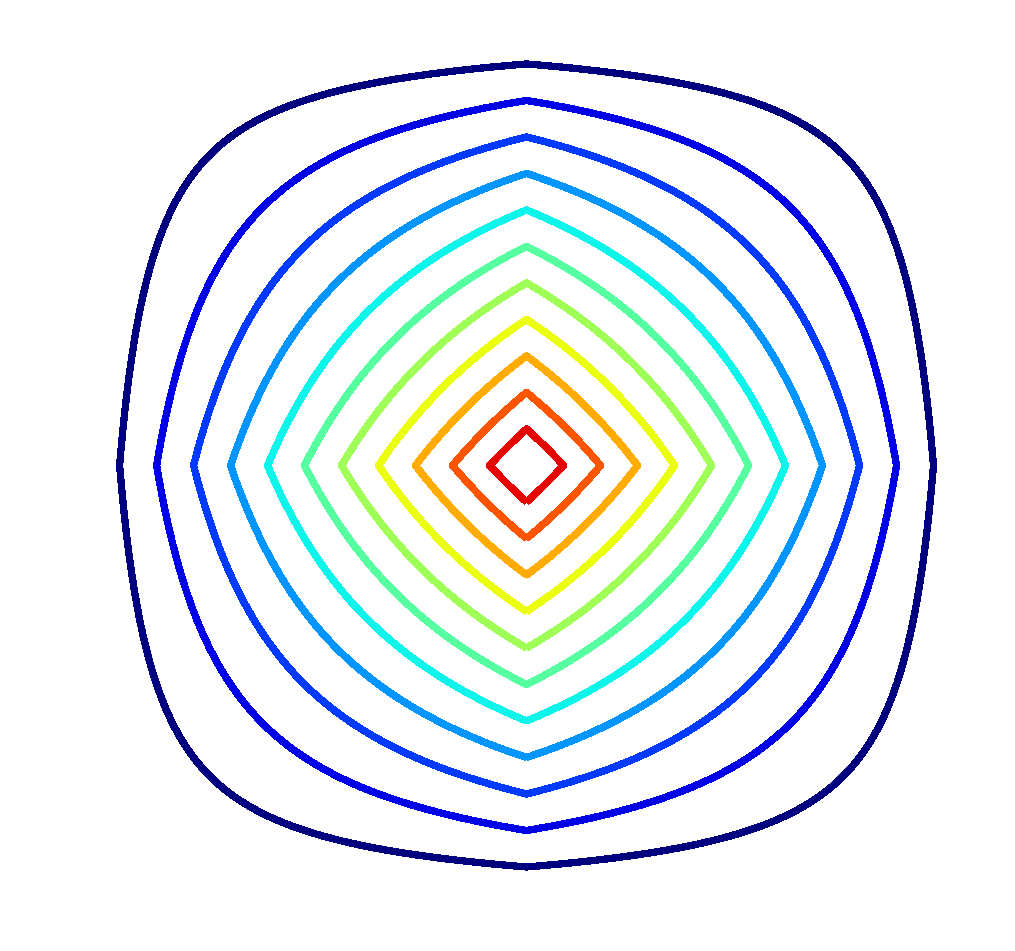
\includegraphics[width=5cm,height=5cm]{figs/shearlets/newmother0} \\
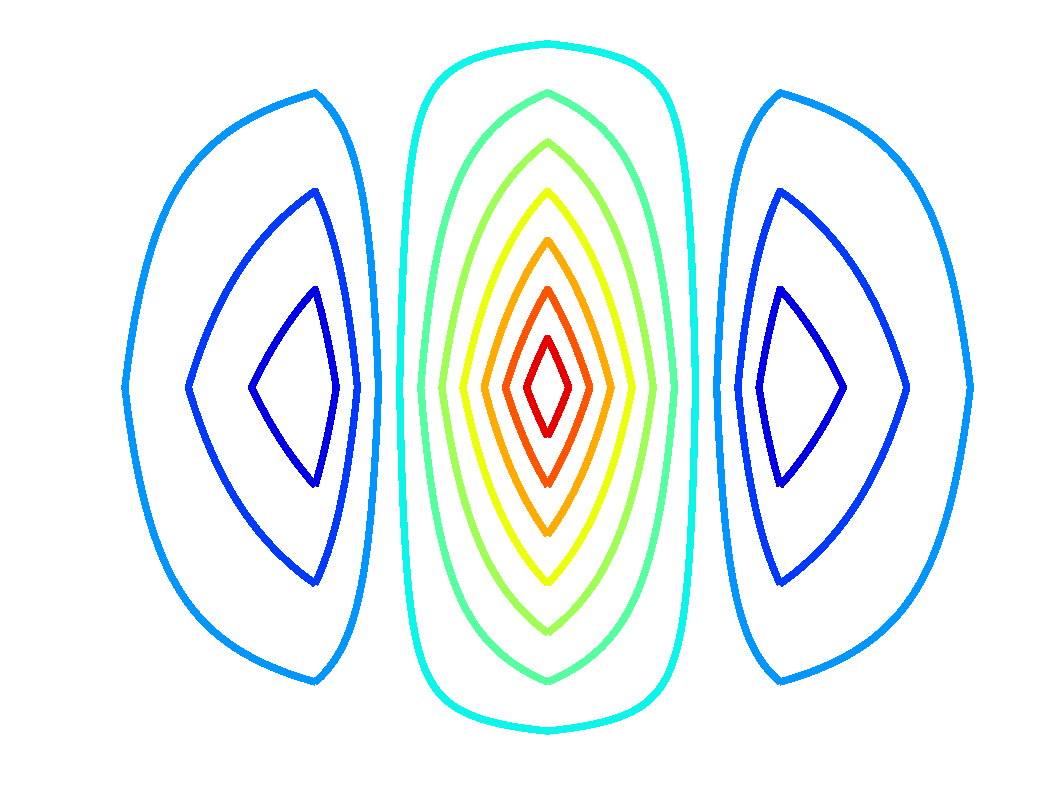
\includegraphics[width=5cm,height=5cm]{figs/shearlets/newmother1}
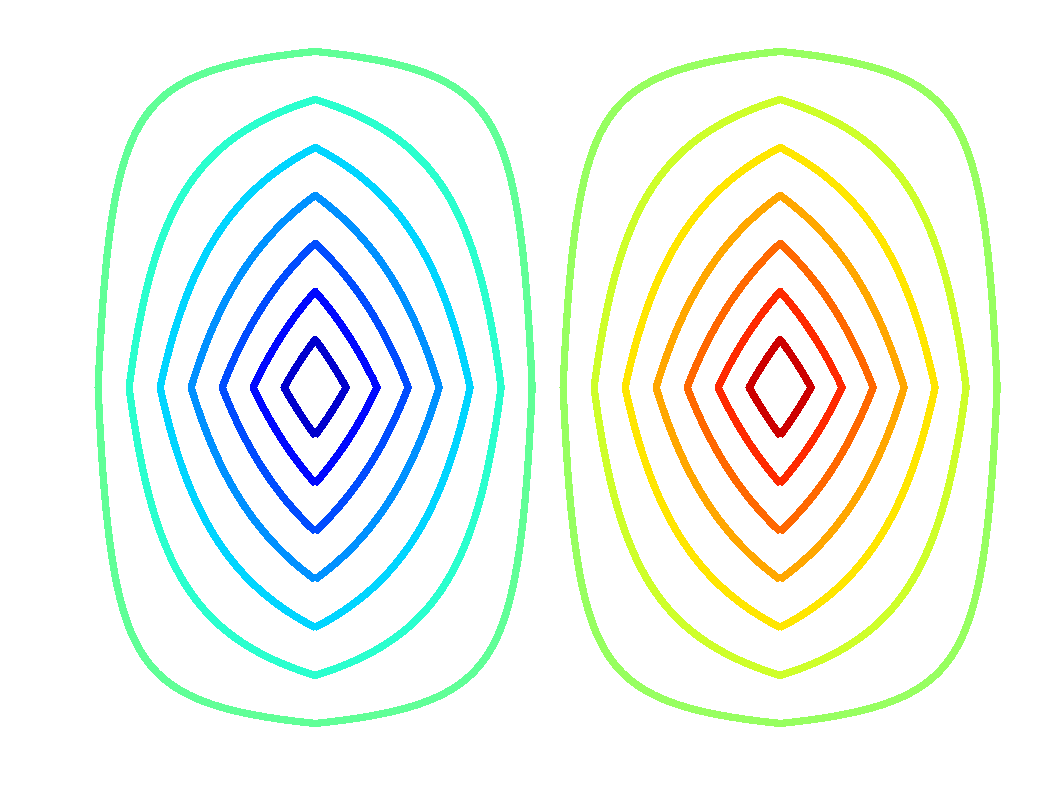
\includegraphics[width=5cm,height=5cm]{figs/shearlets/newmother2}
\caption{Mother shearlets for level $j=0$ (top) and $j>0$ (bottom).}
\label{fig:mothers}
\end{figure}

\subsection{Boundary conditions} \label{sec:boundarycond}

Since shearlets in general are not zero on the inflow boundary $\Gamma_-$, they cannot be used as-is to solve
\eqref{eqn:trp}. To remedy this, we introduce a multiplier function $z(\Bx)$ that is zero on $\Gamma_-$, and
nonzero everywhere else.

For the easiest test cases, namely constant transport directions $\Bv(\Bx)$, the construction of $z$ is
straightforward. We have, for example,
\[
    \Bv(\Bx) \equiv (1,1) 
    \implies \Gamma_- = [0,1] \times \{0\} \cup \{0\} \times [0,1]
    \quad \text{so} \quad
    z(\Bx) = x_1 x_2,
\]
or if $\Bv$ is aligned with one of the axes,
\[
    \Bv(\Bx) \equiv (0,1)
    \implies \Gamma_- = \{0\} \times [0,1]
    \quad \text{so} \quad
    z(\Bx) = x_2.
\]
It will not be necessary for us, and it is beyond the scope of this text, to pursue the construction of $z$
for more sophisticated cases. We mention, however, that it is desirable to keep $z$ as simple and smooth as
possible, both to preserve the approximating properties of shearlets and not to impose unreasonable conditions
on quadrature rules.

Once a suitable boundary multiplier function has been found, we simply substitute $z\Psi$ for every shearlet
$\Psi$, forming a new basis (for a different function space, a subspace of $V_0$) that conforms to the
boundary conditions. This treatment closely conforms to the partition of unity method (see \cite{Melenk96} and
\cite{Babuska97}).

We will also consider periodic boundary conditions, where this construction is unnecessary.

\subsection{Translations} \label{sec:translations}

It remains to specify the translation parameter $\Bc$. Assume that the fundamental wavelets and scaling
functions $\psi$ and $\varphi$ are piece-wise linear on a mesh with exactly $W_x$ and $W_y$ equally sized
intervals, respectively. That is,
\[
    \psi|_{\left(-\frac{1}{2}+\frac{i}{W_x},-\frac{1}{2}+\frac{i+1}{W_x}\right)}
    \qquad \text{and} \qquad
    \varphi|_{\left(-\frac{1}{2}+\frac{l}{W_y},-\frac{1}{2}+\frac{l+1}{W_y}\right)}
\]
are linear for all $0 \leq i < W_x$ and $0 \leq l < W_y$.

Now fix the level $j$ and let for the moment $k=0$. Then our shearlets $\aPsi{\cdot}{\cdot}{\cdot}{j}{0}$ are
piece-wise bilinear on a tensor product mesh which is uniform of resolution $\nicefrac{s_x^{-j}}{W_x}$ and
$\nicefrac{s_y^{-j}}{W_y}$ in the $x$- and $y$-directions respectively. If $s_x$ and $s_y$ are integers, this
mesh lines up perfectly with the boundaries of the domain.\footnote{If $s_x=\nicefrac{p}{q}$ is rational, the
mesh will also line up in the $x$-direction for those levels $j$ where $q^j$ divides $W_x$, if any (and
correspondingly in the $y$-direction.)}

As a consequence, we can represent all functions that are bilinear on this mesh by choosing translations
spaced by $\nicefrac{s_x^{-j}}{W_x}$ in the first direction, and $\nicefrac{s_y^{-j}}{W_y}$ in the second,
whence
\[
    \Bc \in \left\{\begin{pmatrix}
                    L(j) + \nicefrac{\alpha}{s_x^jW_x} \\ 
                    D(j) + \nicefrac{\beta}{s_y^jW_y}
                 \end{pmatrix} \;:\;
          0 \leq \alpha < R(j), \;\; 0 \leq \beta < U(j) \right\}.
\]
This set of translations is valid for the first cone $r=0$, and must be mirrored accordingly if $r=1$. It is
described by means of four helper functions: $(L(j), D(j))$ for the position of the ``bottom left'' shearlet,
and the maximal displacements $R(j)$ and $U(j)$ in each direction. These values are derived so that given any
level $j$, cone $r$ and translate $\Bc$, there is at least one shear $k$ so that $\aPsi{\cdot}{\Bc}{r}{j}{k}$
has support intersecting the domain $\Omega$. From this we find
\[ 
    L(j)=\begin{cases} \frac{s_x^{-j}}{W_x}-\frac{s_x^{-j} + s_y^{-j}}{2}, & j>0, \\ 0, & j=0, \end{cases}
    \qquad 
    R(j)=[1-2L(j)]s_x^jW_x+1,
\]
and
\[ 
    D(j) = 0,\qquad 
    U(j) = s_y^jW_y+1.
\]
We offer some illustrations in Figures~\ref{fig:extremeshearlets} and \ref{fig:translations} for the case
$W_x=4$, $W_y=4$ and $s_x=4$, $s_y=2$. 

For periodic boundary conditions, things become much simpler.
\[
    L(j) = D(j) = 0, \qquad R(j) = s_x^jW_x, \qquad U(j) = s_y^jW_y.
\]
Some care will be needed if the wavelets and scaling functions $\psi_\cdot$ and $\varphi_\cdot$ have different
structures (i.e. if $W_x$ and $W_y$ depend on $m$). Our construction does not allow coupling between the
translations $\Bc$ and the mother shearlets $m$. In this case, it would be most appropriate to let
$W_x=\lcm_m\{W_x(m)\}$ and $W_y=\lcm_m\{W_y(m)\}$ (least common multiple), so long as these numbers are not
prohibitively large.

\begin{figure}
\centering
\begin{tikzpicture}[scale=4]
    \begin{scope}[scale=0.04]
    \begin{scope}[cm={8,0,0,8,(0,0)}]
    \draw[color=blue,line width=1pt] (1,1) -- (-1,1) -- (-1,-1) -- (1,-1) -- (1,1);
    \end{scope}
    \begin{scope}[cm={2,0,-4,4,(-13,8)}]
    \draw[line width=1pt] (1,1) -- (-1,1) -- (-1,-1) -- (1,-1) -- (1,1);
    \end{scope}
    \begin{scope}[cm={2,0,4,4,(13,8)}]
    \draw[line width=1pt] (1,1) -- (-1,1) -- (-1,-1) -- (1,-1) -- (1,1);
    \end{scope}
    \begin{scope}[cm={2,0,4,4,(-13,-8)}]
    \draw[line width=1pt] (1,1) -- (-1,1) -- (-1,-1) -- (1,-1) -- (1,1);
    \end{scope}
    \begin{scope}[cm={2,0,-4,4,(13,-8)}]
    \draw[line width=1pt] (1,1) -- (-1,1) -- (-1,-1) -- (1,-1) -- (1,1);
    \end{scope}
    \begin{scope}[cm={4,-4,0,2,(8,-13)}]
    \draw[line width=1pt] (1,1) -- (-1,1) -- (-1,-1) -- (1,-1) -- (1,1);
    \end{scope}
    \begin{scope}[cm={4,4,0,2,(8,13)}]
    \draw[line width=1pt] (1,1) -- (-1,1) -- (-1,-1) -- (1,-1) -- (1,1);
    \end{scope}
    \begin{scope}[cm={4,4,0,2,(-8,-13)}]
    \draw[line width=1pt] (1,1) -- (-1,1) -- (-1,-1) -- (1,-1) -- (1,1);
    \end{scope}
    \begin{scope}[cm={4,-4,0,2,(-8,13)}]
    \draw[line width=1pt] (1,1) -- (-1,1) -- (-1,-1) -- (1,-1) -- (1,1);
    \end{scope}
    \end{scope}
\end{tikzpicture}
\caption{The extreme shearlets for $j=1$, $s_x=4$, $s_y=2$. The blue square represents $\Omega$.}
\label{fig:extremeshearlets}
\end{figure}

\definecolor{purple}{rgb}{0.75,0,0.5}

\begin{figure}
\centering
\begin{tikzpicture}[scale=4]
    \begin{scope}[scale=0.06]
    \begin{scope}[cm={8,0,0,8,(0,0)}]
    \draw[color=blue,line width=0.5pt] (1,1) -- (-1,1) -- (-1,-1) -- (1,-1) -- (1,1);
        \begin{scope}[scale=0.125]
            \foreach \x in {-13,-12,...,13} { \foreach \y in {-8,-4,...,8} { 
                \fill[color=red] (\x,\y) circle (0.18); 
                \fill[color=blue] (\y,\x) circle (0.18); 
            } }
            \foreach \x in {-8,-4,...,8} { \foreach \y in {-8,-4,...,8} {
                \fill[color=purple] (\x,\y) circle (0.19);
            } }
        \end{scope}
    \end{scope}
    \end{scope}
\end{tikzpicture} \\
\caption{Translation points for $j=1$, $s_x=4$, $s_y=2$, $W_x=4$, $W_y=2$. The red points are for $r=0$ and
the blue points are for $r=1$.}
\label{fig:translations} 
\end{figure}

\subsection{Numbers of shearlets}

Let us now consider the asymptotic complexity of this method by counting the number of shearlets $N(j)$ at
each level $j$. From the previous analysis, we get for $j>0$ (assuming $\nicefrac{s_x}{s_y}$ an integer):
\begin{multline*}
    N(j) = 2 M(j)
           \underbrace{\left(1+2\left(\frac{s_x}{s_y}\right)^{j-1}\right)}_{\text{shears}}
           \underbrace{\left(s_y^jW_y(j) + 1\right)}_{\text{up-down}} \\
           \underbrace{\left(\left(1+s_x^j\left(1+s_y^{-j}\right)\right)W_x(j)-1\right)}_{\text{left-right}}.
\end{multline*}
where $M(j)$ is the number of mother shearlets at level $j$, and $W_x(j)$ and $W_y(j)$ have the meaning given
in Section~\ref{sec:translations}. Thus, if $M,S,W$ are all asymptotically bounded, we obtain
\[
    N(j) \sim s_x^{2j},
\]
which, for the choices of $(s_x,s_y)$ listed earlier, reduces to rates of $16^j$ and $4^j$. The exact numbers
for levels $j=1,\ldots,6$ are listed in Table~\ref{tbl:numlets}, given the previously described mother
shearlets---that is, $M(0)=1$ and $M(j)=2$ for $j>0$.

Of course, this is an extremely rapid growth. Performing a full space solution with even very modest
resolution $j$ is quite challenging, not only due to solving the linear system, but also because assembly is a
nontrivial problem (as we shall see). The main hope for shearlets lie in their naturally adaptive properties.
One might hope that most active coefficients belong to shearlets which are aligned with the transport
direction $\Bv(\Bx)$, so that the vast majority of the search space can be dispensed with.

\begin{table}
\centering
\def\arraystretch{1.4}
\begin{tabular}{r@{\qquad}l@{\qquad}l}
$j$ & $(4,2)$ & $(2,1)$ \\
\hline $1$ & $8.10\cdot10^{2}M(1)$ & $3.42\cdot10^{2}M(1)$ \\
\hline $2$ & $7.47\cdot10^{3}M(2)$ & $1.05\cdot10^{3}M(2)$ \\
\hline $3$ & $8.90\cdot10^{4}M(3)$ & $3.62\cdot10^{3}M(3)$ \\
\hline $4$ & $1.22\cdot10^{6}M(4)$ & $1.34\cdot10^{4}M(4)$ \\
\hline $5$ & $1.81\cdot10^{7}M(5)$ & $5.13\cdot10^{4}M(5)$ \\
\hline $6$ & $2.79\cdot10^{8}M(6)$ & $2.01\cdot10^{5}M(6)$ \\
\end{tabular}
\caption{Number of shearlets per level. $(s_x,s_y)=(4,2)$ on the left and $(s_x,s_y)=(2,1)$ on the right. In
both cases, $W_x(j)=2$ and $W_y(j)=4$.} \label{tbl:numlets}
\end{table}

\section{Algorithms} \label{sec:algorithms}

In the following, we will describe in some detail a basic implementation for a shearlet solver for
\eqref{eqn:trp}. There are no significant new ideas here, but it will perhaps serve to highlight some typical
difficulties faced.

At the time this work was done, this was the only shearlet implementation available intended for the solution
of PDEs. Since then, other work has shown promise using different strategies, among them \cite{ObermeierXX}.

\subsection{Numbering}

We number shearlets according to a hierarchy of parameters. As the only open-ended parameter, and since the
ranges of other parameters depend on it, naturally $j$ must be most significant. The order of the others is
not overly important.

In the following, we will describe shearlets in algorithms as a single variable (usually $s$ or $t$), which
can be assumed to work as a structure, and that sub-fields can be accessed by dot-notation such as $s.j$. We
will also speak of $s$ as the shearlet itself (i.e. the mathematical function). The meaning should in either
case be clear from the context.

\subsection{Transformation} \label{sec:transformation}

For our purposes we need to be able to evaluate shearlets at arbitrary points in $\bbR^2$. This is done using
the transformation technique in \eqref{eqn:trflet}. A function called $\basetrf$ takes a shearlet and produces
the transformation matrix $\BA$ and the translation vector $\Bc$,
\[ 
    (\BA,\Bc) \leftarrow \basetrf(s).
\]
The mapping $\Bx \mapsto \BA(\Bx-\Bc)$ is an affine transformation mapping the square
$[-\nicefrac{1}{2},\nicefrac{1}{2}]^2$ to the support of $s$.

The reason for the name $\basetrf$ is that it will also be useful to have a more general function called
$\trf$ that can produce mappings into subdomains of the support of $s$. Recall that $s$ is defined as an
affine transformation of a tensor product of two piece-wise linear functions, so that $s$ is piece-wise
polynomial with maximal degree $2$. (It is not necessarily piece-wise bilinear, because the shearing will add
squared terms.) By {\em subdomain} we mean the subsets of the support of $s$ on which $s$ is polynomial. These
are numbered as shown in Figure~\ref{fig:subnumbering}.

\begin{figure}
\centering
\begin{tikzpicture}[scale=1.3125]
    \draw[line width=1pt] (-1,-1) -- (1,-1) -- (1,1) -- (-1,1) -- (-1,-1);
    \draw[line width=1pt] (-0.5,-1) -- (-0.5,1);
    \draw[line width=1pt] (0,-1) -- (0,1);
    \draw[line width=1pt] (0.5,-1) -- (0.5,1);
    \draw[line width=1pt] (-1,0) -- (1,0);
    \node at (-0.75,-0.5) {1}; \node at (-0.25,-0.5) {2}; \node at (0.25,-0.5) {3}; \node at (0.75,-0.5) {4};
    \node at (-0.75,0.5) {5}; \node at (-0.25,0.5) {6}; \node at (0.25,0.5) {7}; \node at (0.75,0.5) {8};
    \begin{scope}[cm={1,0,1,1,(-1.5,-2.5)}]
        \draw[line width=1pt] (-1,-1) -- (1,-1) -- (1,1) -- (-1,1) -- (-1,-1);
        \draw[line width=1pt] (-0.5,-1) -- (-0.5,1);
        \draw[line width=1pt] (0,-1) -- (0,1);
        \draw[line width=1pt] (0.5,-1) -- (0.5,1);
        \draw[line width=1pt] (-1,0) -- (1,0);
        \node at (-0.75,-0.5) {1}; \node at (-0.25,-0.5) {2}; \node at (0.25,-0.5) {3}; \node at (0.75,-0.5) {4};
        \node at (-0.75,0.5) {5}; \node at (-0.25,0.5) {6}; \node at (0.25,0.5) {7}; \node at (0.75,0.5) {8};
    \end{scope}
    \begin{scope}[cm={0,1,1,1,(1.2,-2.5)}]
        \draw[line width=1pt] (-1,-1) -- (1,-1) -- (1,1) -- (-1,1) -- (-1,-1);
        \draw[line width=1pt] (-0.5,-1) -- (-0.5,1);
        \draw[line width=1pt] (0,-1) -- (0,1);
        \draw[line width=1pt] (0.5,-1) -- (0.5,1);
        \draw[line width=1pt] (-1,0) -- (1,0);
        \node at (-0.75,-0.5) {1}; \node at (-0.25,-0.5) {2}; \node at (0.25,-0.5) {3}; \node at (0.75,-0.5) {4};
        \node at (-0.75,0.5) {5}; \node at (-0.25,0.5) {6}; \node at (0.25,0.5) {7}; \node at (0.75,0.5) {8};
    \end{scope}
\end{tikzpicture}
\caption{An example of subdomain numbering, where $W_x=4$ and $W_y=2$. The resulting shearlets are piece-wise
polynomial on $W_xW_y=8$ sections.} \label{fig:subnumbering}
\end{figure}

Thus we define a function $\trf(s,i)$ which takes a subdomain number as a second optional argument. If $i$ is
not specified or $i=0$, it is assumed that $\basetrf(s)$ is meant. See Algorithm \ref{alg:trf}.

\begin{algorithm}
\caption{$\trf$ computes $\BA$ and $\Bc$ for a given shearlet and subdomain number.} \label{alg:trf}
\begin{algorithmic}[1]
\REQUIRE Shearlet $s$ and optional subdomain number $0\leq i\leq 8$
\STATE $(\BA,\Bc)\leftarrow \basetrf(s)$
\IF{$i$ is given and $i>0$}
\STATE $\Bd\leftarrow \left(\frac{1}{W_x}\left(\left(i-1\modd W_x\right)+\frac{1}{2}\right)-\frac{1}{2},\quad
        \frac{1}{W_y}\left(\lfloor\frac{i-1}{W_x}\rfloor+\frac{1}{2}\right)-\frac{1}{2}\right)^\intercal$
\STATE $\Bc\leftarrow \BA^{-1}\Bd+\Bc$
\STATE $\BA\leftarrow \begin{pmatrix} W_x&\\&W_y \end{pmatrix} \cdot \BA$
\ENDIF
\RETURN $(\BA,\Bc)$
\end{algorithmic}
\end{algorithm}

In the following, we will often be concerned with the polygon defined by the support of a given shearlet, or
one of its subdomains. We will consider polygons as $2\times n$-matrices of vertices $(p_1,p_2,\ldots,p_n)$
numbered counterclockwise, where $p_n\neq p_1$. A useful convenience is the function $\corners$, which
computes these vertices by transforming the corners of the reference square $[-1/2,1/2]^2$, see Algorithm
\ref{alg:corners}. If no shearlet is given, it returns the corners of the computational domain.

\begin{algorithm}
\caption{$\corners$ computes the vertices of a shearlet support or subdomain.} \label{alg:corners}
\begin{algorithmic}[1]
\REQUIRE Optional shearlet $s$ and optional subdomain number $0\leq i\leq 8$
\IF {$s$ is not given}
\RETURN $\begin{pmatrix} 0&1&1&0 \\ 0&0&1&1 \end{pmatrix}$
\ENDIF
\STATE $(\BA,\Bc)\leftarrow \trf(s,i)$
\STATE $\Bp\leftarrow \frac{1}{2} \BA^{-1}\begin{pmatrix} -1&1&1&-1 \\ -1&-1&1&1 \end{pmatrix} + \Bc$
\IF {$s.r=1$}
\STATE Reverse the order of $\Bp$
\ENDIF
\RETURN $\Bp$
\end{algorithmic}
\end{algorithm}

\subsection{Assembly strategy} \label{ssec:assemblystrat}

\subsubsection{Stiffness matrix}

Given a bilinear form $\blfa(\cdot,\cdot)$ we want to compute the corresponding stiffness matrix for a given
index set $\cI$ of shearlets. In an ordinary hierarchical setting (e.g. with hat functions), one would rely on
a {\em refinement relation} that expresses a function as a linear combination of functions on the next level.
This would allow us to compute the stiffness matrix for the highest level only, and then use the refinement
relation to fill out the coarser matrices. There are several problems with this.

\begin{enumerate}
\item The number of shearlets on each level increases very fast, asymptotically (in our worst case) $16^j$,
compared to the more conventional $4^j$. The saved effort from not having to directly calculate the coarse
levels becomes almost negligible.

\item In a more traditional setting, such as with triangular elements and hat functions, it is possible to
assemble the matrix in time that scales linearly with the number of elements, as this circumvents the
necessity of having to check if the supports of two functions overlap. No such shortcut is readily available
to us in the shearlet case.\footnote{It is true that there are simple methods that can identify a number of
negatives (no intersection), such as checking the center and diameter of shearlet supports, or cheap
intersection checking routines. However, these cases still have to be {\em tested}, and moreover, the
stiffness matrix will nevertheless not be sparse (although it might be compressible).}

\item The primary motivation for implementing a shearlet basis/frame is to employ adaptive methods, and thus
to be able to dispense with a large number of fine-level basis functions. The refinement relation strategy
outlined would negate to some extent the advantages offered by adaptivity.
\end{enumerate}

Due to this, for the time being, we will fall back to the primitive loop which merely iterates over all pairs
of shearlets and computes their corresponding matrix entry. Some speedup is possible in this step since our
matrix is symmetric. Parallelization ought to be considered here.

How, then, do we go about computing $\blfa(s_i,s_j)$? The most obvious approach is straightforward.

\begin{enumerate}
\item Identify the vertices of the supports of $s_i$ and $s_j$ using the function $\corners$.
\item Check if the supports intersect. If they do not, return $0$.
\item If the supports intersect, loop over pairs of subdomains of the supports of $s_i$ and $s_j$. Compute
the intersection of this pair if it is nonempty. This produces a set of nonempty disjoint polygons $P_k$
whose union is the intersection of supports of $s_i$ and $s_j$, and which has the property that both $s_i$ and
$s_j$ are polynomial on any $P_k$.
\item Further divide each $P_k$ into a set of triangles. On each triangle, form a quadrature rule. Take the
union of these quadrature rules as a quadrature rule for the intersection of the supports of $s_i$ and $s_j$.
\end{enumerate}

Once the quadrature rule is in hand, the integrand of the bilinear form $\blfa$ can be evaluated on the
quadrature points and summed up accordingly.

There should be a basic choice of quadrature rule defined on a reference triangle, which can then be
transformed.  This part is essentially identical to triangular Lagrangian FEM. If there are no variable
coefficients, we can achieve exact integration with a quadrature rule of sufficiently high order. If there
{\em are} variable coefficients, the case becomes a little more complicated, which we discuss in
Section~\ref{sec:error-in-quadrature}.

This strategy relies heavily on reliable routines for checking and computing intersections between convex
polygons. Experiments suggest that most of the processing time is spent doing operations like these, and care
should be taken to implement these properly (see Section~\ref{sec:intersections}).\footnote{There is a fair
amount of overlap available. For example if $s_i$ and $s_j$ give rise to a quadrature rule $q$, then
translates of $s_i$ and $s_j$ (by the same vector) give rise to translates of $q$, unless these translates
intersect with the boundary of the domain.}

We now assume the existence of these functions:

\begin{enumerate}
\item A function $\checkintersection(s,t)$ for checking if the supports of shearlets $s$ and $t$ intersect at
all.
\item A function $\computeintersection(p,q)$ for computing intersections between two convex polygons $p$ and
$q$.
\item A function $\splitpolygon(p)$ for reducing a polygon $p$ to a collection of triangles.
\item A function $\transformquadrule(q,p)$ for transforming a quadrature rule $q$ defined on a reference
triangle onto the triangle $p$.
\end{enumerate}

The algorithms for checking and computing intersections are discussed further in
Section~\ref{sec:intersections}. The $\splitpolygon$ function can be implemented in a myriad of different
ways, one of which is described in Algorithm~\ref{alg:splitpolygon}. This algorithm splits a polygon as shown
in Figure~\ref{fig:splitpolygon}, where the red vertex is vertex number $1$. The algorithm alternates between
adding a triangle on the ``right'' or ``left'' side, and keeps track of the next unused vertex on both sides.
No new vertices are introduced.

Algorithm~\ref{alg:builddquadrule} contains pseudo-code for the $\builddquadrule$ function, which builds a
quadrature rule for the intersection of two shearlet supports. 

\begin{figure}
\centering
\begin{tikzpicture}
    \coordinate (p1) at (0,0);
    \coordinate (p2) at (2,-0.3);
    \coordinate (p3) at (3.5,0.5);
    \coordinate (p4) at (4.25,1.75);
    \coordinate (p5) at (4,2.7);
    \coordinate (p6) at (3,3);
    \coordinate (p7) at (1.7,3);
    \coordinate (p8) at (0.4,2.3);
    \coordinate (p9) at (-0.5,1);
    \draw[line width=1pt] (p1) -- (p2) -- (p3) -- (p4) -- (p5) -- (p6) -- (p7) -- (p8) -- (p9) -- (p1);
    \fill[color=red] (p1) circle (3pt);
    \fill (p2) circle (3pt); \fill (p3) circle (3pt); \fill (p4) circle (3pt); \fill (p5) circle (3pt); 
    \fill (p6) circle (3pt); \fill (p7) circle (3pt); \fill (p8) circle (3pt); \fill (p9) circle (3pt);
    \draw[dashed, line width=1pt] (p9) -- (p2) -- (p8) -- (p3) -- (p7) -- (p4) -- (p6);
\end{tikzpicture}
\caption{Splitting a polygon into triangles. The red vertex is number one.} \label{fig:splitpolygon}
\end{figure}

\begin{algorithm}
\caption{$\splitpolygon$ divides a polygon $p$ into a collection of triangles.}
\label{alg:splitpolygon}
\begin{algorithmic}[1]
\REQUIRE $2\times N$ matrix $p$ denoting a polygon
\STATE start\ $\leftarrow3$, end\ $\leftarrow1$, right\ $\leftarrow$\ false, $T\leftarrow \left\{\begin{pmatrix}
p_{\cdot,1}&p_{\cdot,2}&p_{\cdot,N} \end{pmatrix}\right\}$ \WHILE{$\mathrm{start}+\mathrm{end}\leq N$}
\IF{right}
\STATE $T\leftarrow T\cup\left\{\begin{pmatrix}
p_{\cdot,\mathrm{start}-1}&p_{\cdot,\mathrm{start}}&p_{\cdot,N-\mathrm{end}+1} \end{pmatrix}\right\}$
\STATE $\text{start} \leftarrow \text{start} + 1$
\ELSE
\STATE $T\leftarrow T\cup\left\{\begin{pmatrix}
p_{\cdot,\mathrm{start}-1}&p_{\cdot,N-\mathrm{end}}&p_{\cdot,N-\mathrm{end}+1} \end{pmatrix}\right\}$
\STATE $\text{end} \leftarrow \text{end} + 1$
\ENDIF
\STATE $\text{right} \leftarrow \neg\text{right}$
\ENDWHILE
\end{algorithmic}
\end{algorithm}

\begin{algorithm}
\caption{$\builddquadrule$ constructs a quadrature rule for the intersection of the supports of two shearlets
$s$ and $t$.}
\label{alg:builddquadrule}
\begin{algorithmic}[1]
\REQUIRE Shearlets $s$, $t$ and basic quadrature rule $q$
\STATE $r\leftarrow \emptyset$
\FOR {$i,j\in\{1,\ldots,8\}$}
\STATE $p\leftarrow\corners(s,i)$
\STATE $q\leftarrow\corners(t,j)$
\STATE $B\leftarrow\splitpolygon(\computeintersection(p,q))$
\FOR {$c\in B$}
\STATE $r\leftarrow r\cup\left\{\transformquadrule(q,c)\right\}$
\ENDFOR
\ENDFOR
\end{algorithmic}
\end{algorithm}

%\begin{algorithm}
%\caption{{$\evalblf$} evaluates a bilinear form.} \label{alg:evalblf}
%\begin{algorithmic}[1]
%\REQUIRE Shearlets $s$, $t$, basic quadrature rule $q$ and a function $f(s,t,x)$ for evaluating the integrand
%of a bilinear form at a point $x$.
%\IF {$\checkintersection(s,t)$}
%\STATE $q\leftarrow\builddquadrule(s,t,q)$
%\STATE $r\leftarrow 0$
%\FOR {quadrature point $x$ with weight $w$ $\in q$}
%\STATE $r\leftarrow r+w\cdot f(s,t,x)$
%\ENDFOR
%\RETURN r
%\ELSE
%\RETURN 0
%\ENDIF
%\end{algorithmic}
%\end{algorithm}

\subsubsection{Load vector}

For evaluating the right hand side load vector $\lfl(\cdot)$ the strategy is mostly the same, except we can
ignore most of the intersection checking. The function $\buildsquadrule$ mirrors $\builddquadrule$, and its
pseudo-code is presented in Algorithm~\ref{alg:buildsquadrule}.

\begin{algorithm}
\caption{$\buildsquadrule$ constructs a quadrature rule for the support of a shearlet $s$.}
\label{alg:buildsquadrule}
\begin{algorithmic}[1]
\REQUIRE Shearlet $s$ and basic quadrature rule $q$
\STATE $r\leftarrow \emptyset$
\FOR {$i\in\{1,\ldots,8\}$}
\STATE $p\leftarrow\corners(s,i)$
\STATE $B\leftarrow\splitpolygon(p)$
\FOR {$c\in B$}
\STATE $r\leftarrow r\cup\transformquadrule(q,c)$
\ENDFOR
\ENDFOR
\end{algorithmic}
\end{algorithm}

%\begin{algorithm}
%\caption{{$\evallf$} evaluates a linear form.} \label{alg:evallf}
%\begin{algorithmic}[1]
%\REQUIRE Shearlet $s$, basic quadrature rule $q$ and a function $f(s,x)$ for evaluating the integrand of a
%bilinear form at a point $x$.
%\STATE $q\leftarrow\buildsquadrule(s,q)$
%\STATE $r\leftarrow 0$
%\FOR {quadrature point $x$ with weight $w$ $\in q$}
%\STATE $r\leftarrow r+w\cdot f(s,x)$
%\ENDFOR
%\RETURN r
%\end{algorithmic}
%\end{algorithm}

\subsubsection{Intersections} \label{sec:intersections}

Our method relies on computing intersections between many different polygons, or deciding if polygons are
disjoint. There are several algorithms for computing and detecting intersections, see for example
\cite{Toussaint85, Rourke82, Chazelle80}.  These all assume convexity, which is valid in\
our case.

For checking disjointedness, we rely on the {\em separating axis theorem}, which is commonly used in game
programming for collision detection \cite{Gottschalk96}.

\begin{theorem}[Separating Axis Theorem (SAT)] \label{thm:sat}
Let $A,B\subseteq\bbR^2$ be convex sets in $\bbR^2$. Then $A \cap B=\emptyset$ if and only if there exists a
line that separates $A$ from $B$. Moreover, if $A$ and $B$ are polygons with empty intersection, such a
separating line can always be found among the extensions of the edges of $A$ and $B$.
\end{theorem}
\begin{proof}
The first statement is the Hahn-Banach theorem. For the other, assume that $A$ and $B$ are disjoint convex
polygons, and let $\Ba$, $\Bb$ be points of minimal distance between them. If either $\Ba$ or $\Bb$ is not a
vertex, they are points on edges, and the extensions of either of these edges yield a separating line. 

If both $\Ba$ and $\Bb$ are vertices, consider vertex $\Ba$ and the extension of its edges dividing the
space outside of $A$ into three regions as shown in Figure~\ref{fig:sat}, two of which are named $U$ and $L$.
Assume vertex $\Bb$ is not in $L$. 

If none of $B$ intersects $L$, the edge $r$ will be a separating line. If not, define the line $h$ through
$\Bb$ as being parallel to $r$, and the line $g$ through $\Bb$ as being orthogonal to the line through $\Ba$
and $\Bb$. Now, consider the edge from $\Bb$ in the direction of $L$. Since $B$ intersects $L$ and $\Bb$ is
the point of $B$ closest to $A$, this edge must lie in the wedge between lines $h$ and $g$, and so it clearly
gives a separating line. Moreover, if this wedge is empty, we can see that this contradicts the assumption
that $\Bb$ is closest to $A$.

If $\Bb$ is in $L$, it is not in $U$, and the argument works correspondingly.
\end{proof}

\begin{figure}
\centering
\begin{tikzpicture}[scale=0.9]
    \coordinate (a1) at (0,2); \coordinate (a4) at (0,-2);
    \coordinate (a2) at (2,1.2); \coordinate (a2far) at (5,-2.4); \coordinate (a2near) at (1,2.4);
    \coordinate (a3) at (2,-1.2); \coordinate (a3far) at (5,2.4); \coordinate (a3near) at (1,-2.4);
    \coordinate (hfar) at (2,4.1); \coordinate[label=45:$h$] (hnear) at (7,-1.9);
    \coordinate (gfar) at (4,4.5); \coordinate[label=45:$g$] (gnear) at (6,-3.5);
    \coordinate[label={[label distance=3pt]180:$\Ba$}] (a) at (3,0);
    \coordinate[label={[label distance=3pt]0:$\Bb$}] (b) at (5,0.5);
    \draw[line width=1pt] (a1) -- (a2) -- (a) -- (a3) -- (a4);
    \fill (a1) circle (3pt); \fill (a2) circle (3pt); \fill (a) circle (3pt);
    \fill (a3) circle (3pt); \fill (a4) circle (3pt); \fill (b) circle (3pt);
    \draw[dashed, line width=1pt] (a2near) -- (a2far);
    \draw[dashed, line width=1pt] (a3near) -- (a3far);
    \draw[dotted, line width=1pt] (hnear) -- (hfar);
    \draw[dotted, line width=1pt] (gnear) -- (gfar);
    \node at (1,0) {$A$}; \node at (3,-1.5) {$L$}; \node at (3,1.5) {$U$};
    \node at (2.7,0.8) {$r$};
\end{tikzpicture}
\caption{The separating axis theorem (Theorem~\ref{thm:sat}.)} \label{fig:sat}
\end{figure}

The consequence of Theorem~\ref{thm:sat} is that we can decide if two polygons $p$ and $q$ are disjoint by
looping through the edges of one of them (say $p$). If the vertices are ordered counterclockwise, and we
assume that an edge $e$ therefore has a counterclockwise ``direction'', we already know that $p$ lies on the
left side of $e$, so we need only check if $q$ lies entirely on the right, which can be done by checking the
vertices of $q$ (again, because of convexity). At this point, if no separating line has been found, one has to
loop through the edges of $q$ in a similar fashion.

This is expressed in Algorithm~\ref{alg:checkintersection}. Note that it does not actually check if the
polygons intersect in the computational domain. A few false positives do not worry us, however.

\begin{algorithm}
\caption{$\checkintersection$ checks if the supports of two shearlets $s$ and $t$ are disjoint or not. Returns
true if the supports intersect.}
\label{alg:checkintersection}
\begin{algorithmic}[1]
\REQUIRE Shearlets $s$ and $t$
\STATE $p\leftarrow\corners(s)$, $q\leftarrow\corners(t)$
\FOR{$e\in\mathrm{Edges}(p)$} \label{alg:ci:outer}
\STATE $\text{separatingLine}\leftarrow\mathrm{true}$
\FOR{$\Bv\in\mathrm{Vertices}(q)$}
\IF{$\Bv$ is on the left side of $e$}
\STATE $\text{separatingLine}\leftarrow\mathrm{false}$
\BREAK
\ENDIF
\ENDFOR
\IF{\text{separatingLine}}
\RETURN false
\ENDIF
\ENDFOR
\STATE Repeat loop from line \ref{alg:ci:outer} with $p$ and $q$ interchanged
\RETURN true
\end{algorithmic}
\end{algorithm}

For actually {\em computing} the intersection between two polygons we have employed the General Polygon
Clipper (GPC) library from the University of Manchester \cite{GPC}.

For the case of periodic boundary conditions, some more work is needed. Two shearlets that do not intersect in
the non-periodic case can nevertheless intersect if they are periodically extended. For checking the
intersection, it is necessary to translate the domain of the shearlets by $(m,n)$,
$m,n\in\left\{-1,0,1\right\}$, which corresponds to a shift of at most one period in either direction. This
range of $m,n$ can be restricted somewhat if we take into account the diameters of the shearlet supports, and
where the supports are located with respect to one another. For the smallest shearlets, it will be possible to
reduce the number of translations to be checked to one. Also note that in the periodic case there are no false
positives, as {\em every} possible point of intersection is ``in'' the domain.

For computing the intersection in the periodic case, we must construct unions of polygons, which is supported
by GPC.  Given the support of a shearlet, we intersect it, and all its relevant translations, with the
computational domain. This gives us a union of polygons in $[0,1]^2$ representing the support of that
shearlet. Two such unions can be intersected with GPC and the result is also a union of polygons.

\subsubsection{Error in quadrature} \label{sec:error-in-quadrature}

If the bilinear form $\blfa$ does not contain variable coefficients, it will normally be possible to evaluate
the stiffness matrix exactly (up to machine precision) by choosing a basic quadrature rule which is strong
enough. This will also be possible for the right hand side vector if the function $f$ is simple enough. For
many interesting experiments, however, these functions will vary, and so we consider the effect of this.

In a traditional setting with hat functions, and the strategy involving the refinement relation we discussed
in Section~\ref{ssec:assemblystrat}, the largest ``basic unit'' on which we form quadrature rules are
triangles on the finest level. The size of these approach zero as the levels increase, and so the quadrature
error will automatically approach zero as we refine the finite element space.

In our case however, we apply ``raw'' quadrature to every shearlet, including the coarse ones, and so the
quadrature error will not automatically vanish as we refine our space. In this case it will be necessary to
modify $\builddquadrule$ and $\buildsquadrule$ to further subdivide the triangles before transforming the
basic quadrature. We wish to apply quadrature on {\em small} domains only.

With piece-wise linear shearlets and constant coefficients, it is sufficient to use a quadrature rule that can
integrate quartics exactly (each shearlet is a quadratic). On a triangle of width $h$ and height $k$, with
$k>h$, such a quadrature rule would yield an error of $\cO(hk^6)$ if the coefficients are not constant.
Assuming this is a shearlet at level $j$, let us perform $l_j$ additional steps of uniform subdivision to
limit the size of the domains. After this, we have
\[
    h = \frac{1}{2^{l_j}\cdot W_x\cdot s_x^j},\qquad k = \frac{1}{2^{l_j}\cdot W_y\cdot s_y^j}. 
\]
We want the errors from level $j$ and $i$ to be comparable. Thus
\[
    \frac{2^{l_i}\cdot W_x\cdot s_x^i\cdot 2^{6l_i}\cdot W_y^6\cdot s_y^{6i}}
         {2^{l_j}\cdot W_x\cdot s_x^j\cdot 2^{6l_j}\cdot W_y^6\cdot s_y^{6j}} = 1,
\]
which reveals the relationship
\[
    l_i = l_j + \frac{j-i}{7}\log_2\left(s_x\cdot s_y^6\right),
\]
or, indeed, for a general quadrature rule of order $n$,
\[
    l_i = l_j + \frac{j-i}{2n+1}\log_2\left(s_x\cdot s_y^{2n}\right).
\]
When integrating the intersection between two shearlets $s$ and $t$ at different levels, one should subdivide
as indicated by the smallest shearlet, i.e. use $l_{\max\{s.j,\;t.j\}}$ subdivisions.

\subsubsection{Evaluating shearlets and their gradients}

Ultimately, we will need a function for evaluating a shearlet or its gradient at a given point $\Bx$.  We
transform a point $\Bx$ to the square $[-1/2,1/2]^2$ using $\basetrf$, whereupon we can use linear
interpolation to compute the value of a shearlet at that point (recall that mother shearlets are defined as
tensor products of piece-wise linear functions).

For the gradient, this becomes slightly more complicated. First, we note that
\[ 
    \hPsi_m(\Bx) = \psi(x_1)\varphi(x_2) \quad\Longrightarrow\quad 
    \nabla\hPsi_m(\Bx) = \begin{pmatrix} \psi'(x_1)\varphi(x_2) & \psi(x_1)\varphi'(x_2)
    \end{pmatrix}^\intercal, 
\] 
so our problem is reduced to computing the derivative of a piece-wise linear function in one dimension. After
that, the gradient of $\hPsi_m$ can be assembled, and transformed back to ``real'' space using the matrix
$\BA$ from $\basetrf$.

If $\psi(x)$ (say) is given by its values $\psi_i$ at points $x_i$ ordered in increasing order, we can compute
the derivative at some point $x$ by first identifying $j$ such that $x_j\leq x<x_{j+1}$. Then
\[ \psi'(x) = \frac{\psi_{j+1}-\psi_{j}}{x_{j+1}-x_j}. \]
If no such $j$ exists the derivative is zero.\footnote{In general, all functions are assumed to be defined
everywhere and extended indefinitely with zero, even though they are supported locally.}

Again, some modifications are necessary in the periodic case. Before transformation, a point $\Bx$ can be
translated to any other point on a grid $\left\{\Bx+(m,n)\right\}$, and if any of these translates land in the
domain of a shearlet, the value of the shearlet at that point must be taken.

To do this, define $\Bxi$ and $\Bzeta$ as the transformations of $(1,0)$ and $(0,1)$ to the reference square.
Now, the problem is reduced to finding $m,n$ so that
\[
    \hat{\Bx}+m\Bxi+n\Bzeta \in [-\nicefrac{1}{2},\nicefrac{1}{2}]^2.
\]
The key observation is that due to the nature of the transformation matrix $\BA$ (see \eqref{eqn:trflet}),
either $\zeta_2$ or $\xi_2$ will be zero (which one depends on the cone parameter $r$). Assume without loss of
generality that $\xi_2=0$. Then, only $m$ can affect the second coordinate of the translate, and so we can
immediately solve for $m$ or determine that such an $m$ does not exist. With $m$ fixed, solving for $n$ is
equally simple by considering the equation in the first coordinate. Effectively, this becomes a system of
inequalities corresponding to a triangular linear system. See Algorithm~\ref{alg:preparepoints}

\begin{algorithm}
\caption{$\preparepoints$ transforms a point $\Bx$ to a point $\By$ in the reference square (in case of
periodicity, if such a translate can be found).} \label{alg:preparepoints}
\begin{algorithmic}[1]
\REQUIRE Shearlet $s$, point $x$
\STATE $(\BA,\Bc)\leftarrow\basetrf(s)$
\STATE $\By\leftarrow \BA(\Bx-\Bc)$
\IF{periodic}
\STATE $\Bzeta\leftarrow A(\cdot,1)$, $\Bxi\leftarrow A(\cdot,2)$
\IF{$\xi_2\neq0$}
\STATE interchange $\Bzeta$ and $\Bxi$
\ENDIF
\STATE $n_{\min}\leftarrow \lceil-\frac{1}{\zeta_2}(y_2+\frac{1}{2})\rceil$
\STATE $n_{\max}\leftarrow \lfloor-\frac{1}{\zeta_2}(x_2-\frac{1}{2})\rfloor$
\STATE $m_{\min}\leftarrow \lceil-\frac{1}{\xi_1}(x_2+n_{\min}\zeta_1+\frac{1}{2})\rceil$
\STATE $m_{\max}\leftarrow \lfloor-\frac{1}{\xi_1}(x_2+n_{\min}\zeta_1-\frac{1}{2})\rfloor$
\RETURN $y+m_{\min}\Bxi+n_{\min}\Bzeta$ 
\STATE (will be outside $[-\nicefrac{1}{2},\nicefrac{1}{2}]^2$ if $n_{\min}>n_{\max}$ or $m_{\min}>m_{\max}$)
\ELSE
\RETURN $\By$
\ENDIF
\end{algorithmic}
\end{algorithm}

\section{Stability}

We now turn to investigating the stability of the shearlet function systems already discussed. In particular
we are concerned with the effective condition number of the stiffness matrices produced, both for the mass
matrix ($\Bv\equiv\Bzero,\kappa\equiv1$) and the transport matrix ($\kappa\equiv0$, here we have used
$\Bv\equiv(1,1)$). Since the shearlets are linearly dependent, a distinction has to be made between
eigenvalues which are numerically zero and those which are genuinely nonzero. For the most part, the spectra
show distinct gaps, so that this separation is easily made. The effective condition number can then be defined
as the absolute value of the ratio of the largest genuinely nonzero eigenvalue to the smallest. It is
essentially the condition number of the non-degenerate part of the matrix.

The spectra are plotted in Figures \ref{fig:shl_dbl_nper} through \ref{fig:rid_sglhat_per}. Figures
\ref{fig:shl_dbl_nper} and \ref{fig:shl_dbl_per} show the case $(s_x,s_y)=(4,2)$, and Figures
\ref{fig:rid_dbl_nper} and \ref{fig:rid_dbl_per} show the case $(s_x,s_y)=(2,1)$, both for non-periodic and
periodic shearlets. Lastly, Figures \ref{fig:rid_sglhat_nper} and \ref{fig:rid_sglhat_per} show the case
$(s_x,s_y)=(2,1)$ where all wavelets have been replaced by a scaling function (giving a single isotropic
mother ``shearlet'' on all levels). The effective condition numbers are listed in Table~\ref{tbl:shletconds}

As can be seen, there is every indication that the shearlets as constructed do not form a frame, and that the
condition numbers rapidly deteriorate. This makes them effectively useless for numerical experiments. For this
reason, we abandon here the further study of shearlets and turn to more fruitful topics.

It remains an open question whether a stable {\em usable} shearlet frame can be found, and which properties it
may have.

\clearpage

\begin{figure}
\centering
\begin{tabular}{ccc}
& $j=0$ & $j=1$ \\
\rotatebox{90}{\hspace{1.4cm}Mass} 
& 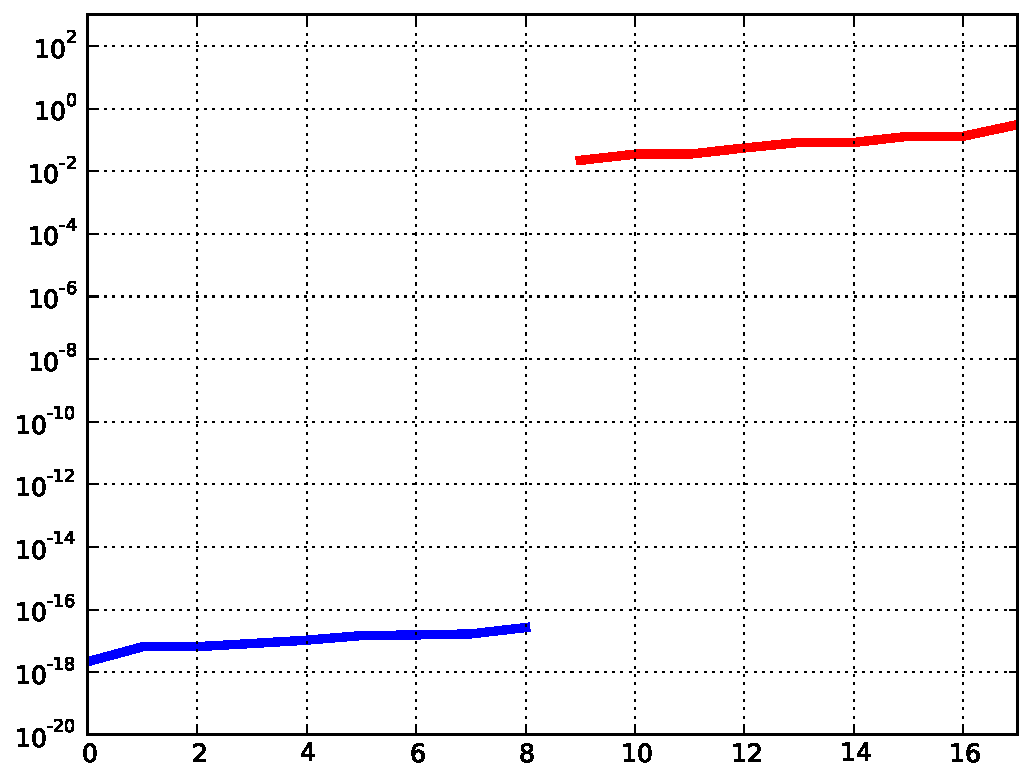
\includegraphics[width=5cm]{figs/shearlets/eigs/shl_dbl_nper_mass0}
& 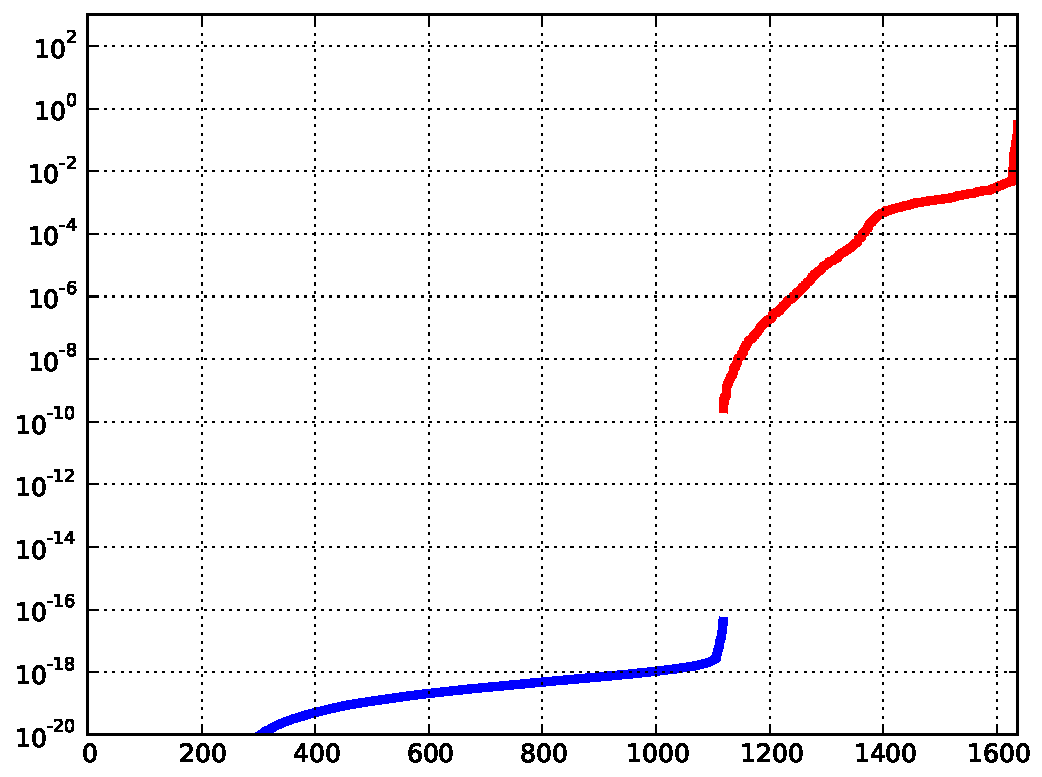
\includegraphics[width=5cm]{figs/shearlets/eigs/shl_dbl_nper_mass1} \\
\rotatebox{90}{\hspace{1.1cm}Transport}
  & 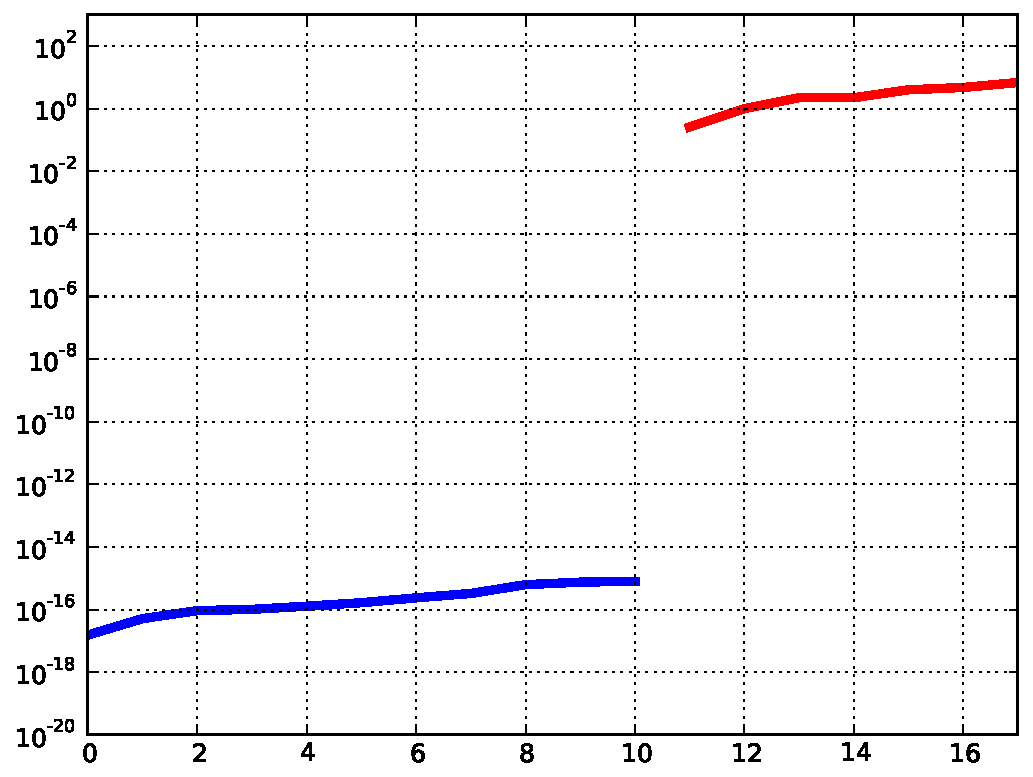
\includegraphics[width=5cm]{figs/shearlets/eigs/shl_dbl_nper_tran0}
  & 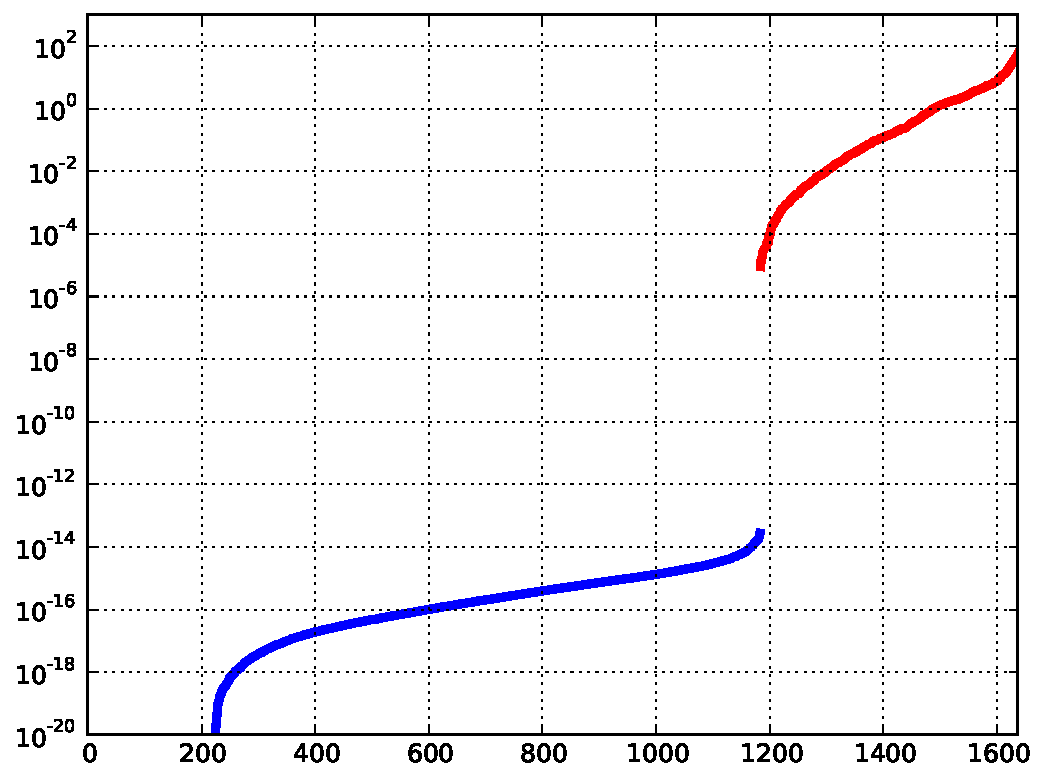
\includegraphics[width=5cm]{figs/shearlets/eigs/shl_dbl_nper_tran1}
\end{tabular}
\caption{Non-periodic, $(s_x,s_y)=(4,2)$.}
\label{fig:shl_dbl_nper}
\end{figure}

\begin{figure}
\centering
\begin{tabular}{ccc}
& $j=0$ & $j=1$ \\
\rotatebox{90}{\hspace{1.4cm}Mass} 
& 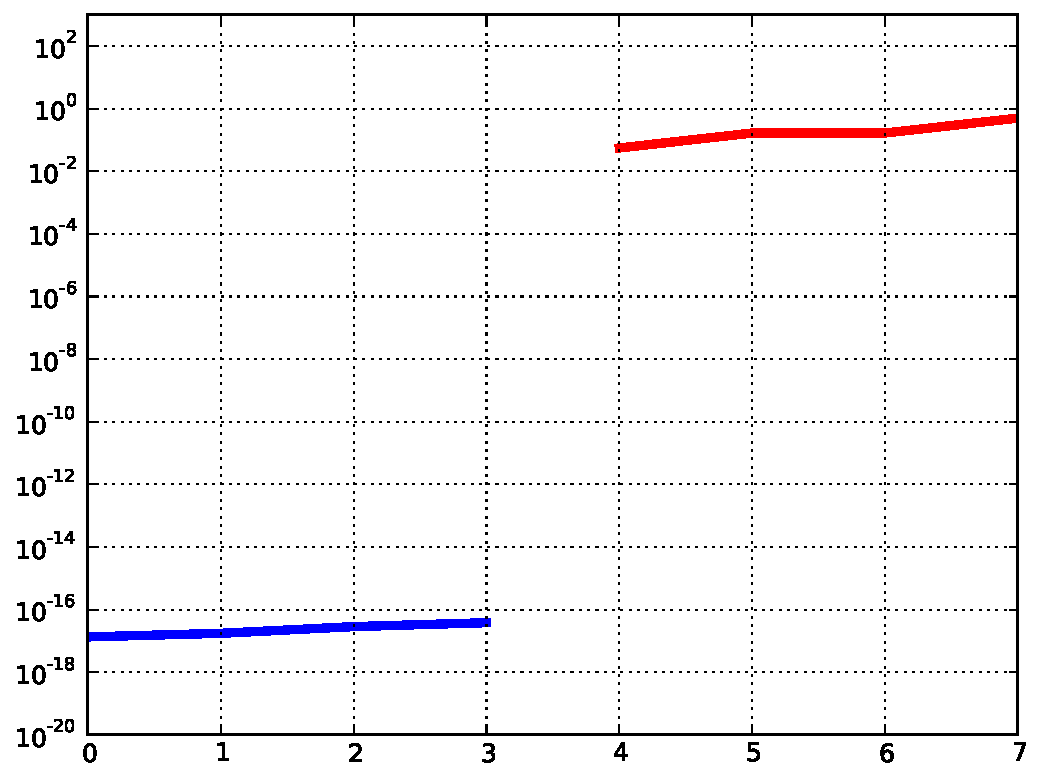
\includegraphics[width=5cm]{figs/shearlets/eigs/shl_dbl_per_mass0}
& 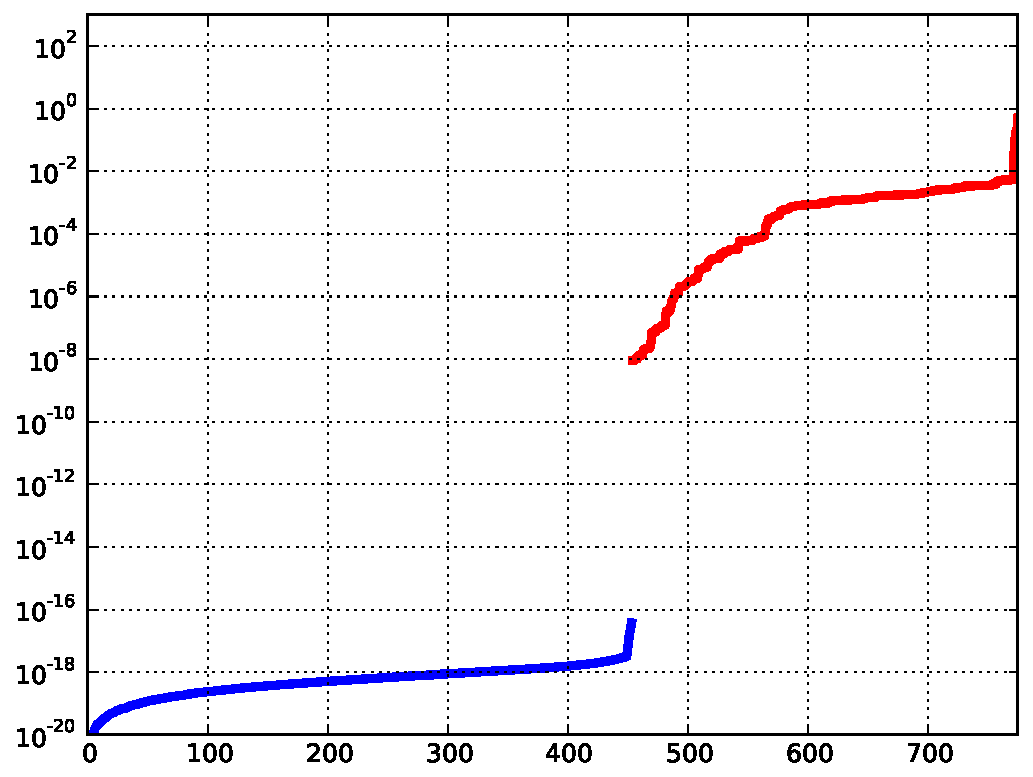
\includegraphics[width=5cm]{figs/shearlets/eigs/shl_dbl_per_mass1} \\
\rotatebox{90}{\hspace{1.1cm}Transport}
& 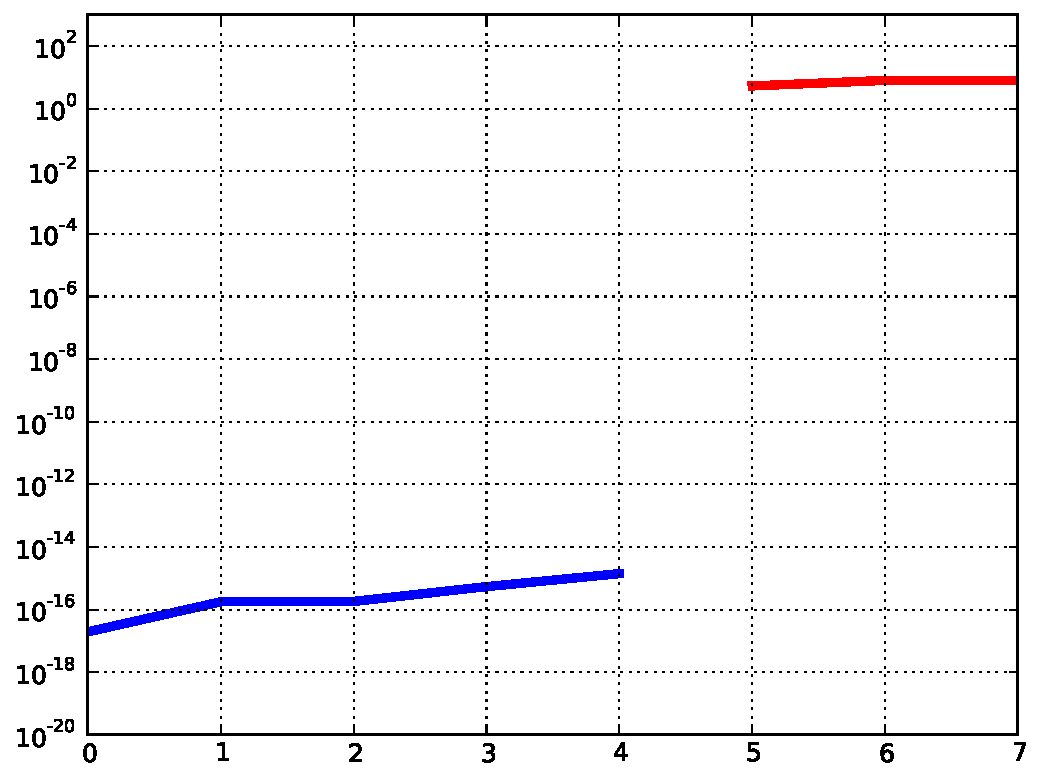
\includegraphics[width=5cm]{figs/shearlets/eigs/shl_dbl_per_tran0}
& 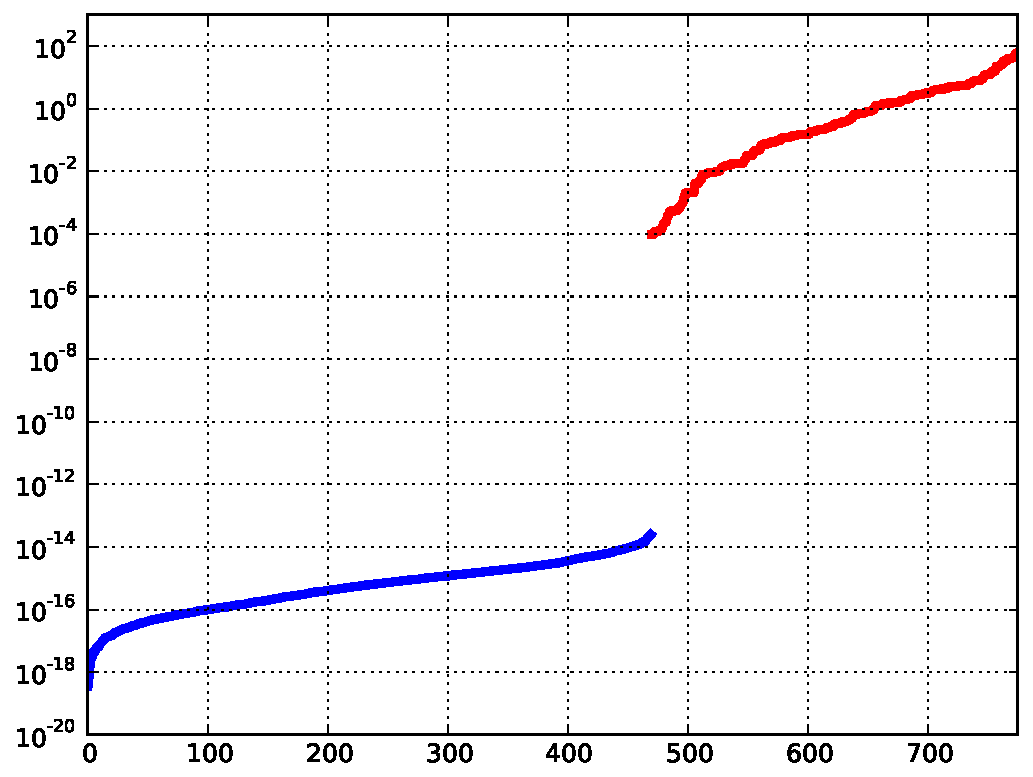
\includegraphics[width=5cm]{figs/shearlets/eigs/shl_dbl_per_tran1}
\end{tabular}
\caption{Periodic, $(s_x,s_y)=(4,2)$.}
\label{fig:shl_dbl_per}
\end{figure}

\begin{figure}
\hspace{-1.3cm}
\centering
\begin{tabular}{cccc}
& $j=0$ & $j=1$ & $j=2$ \\
\rotatebox{90}{\hspace{1.1cm}Mass} 
& 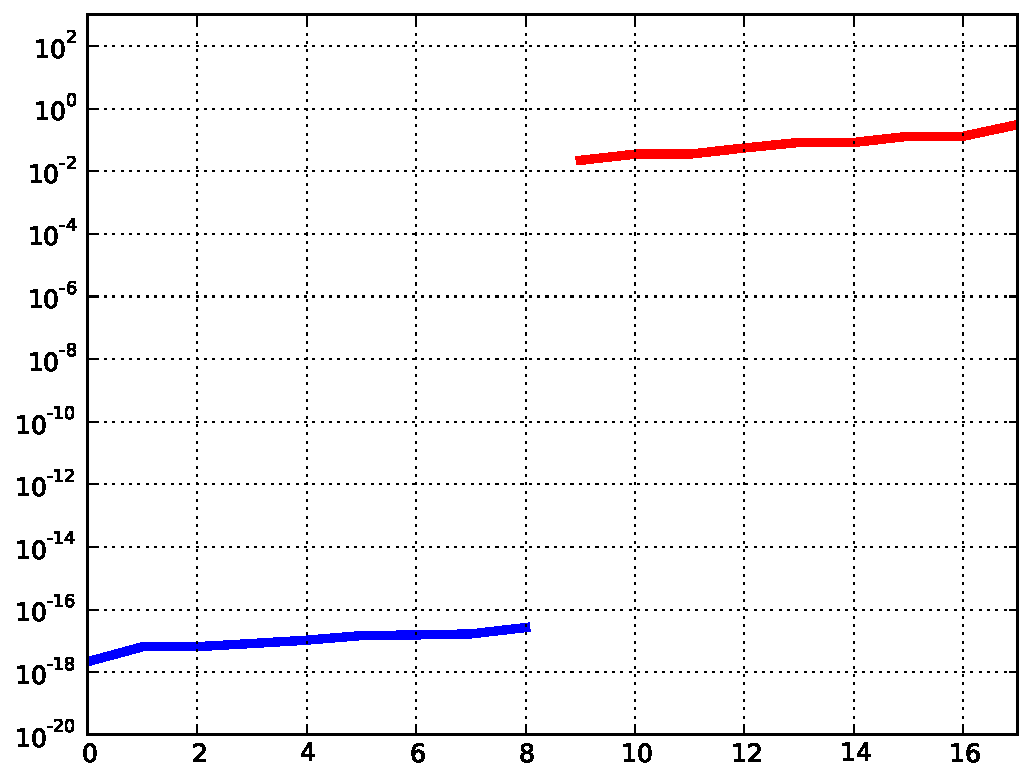
\includegraphics[width=4cm]{figs/shearlets/eigs/rid_dbl_nper_mass0}
& 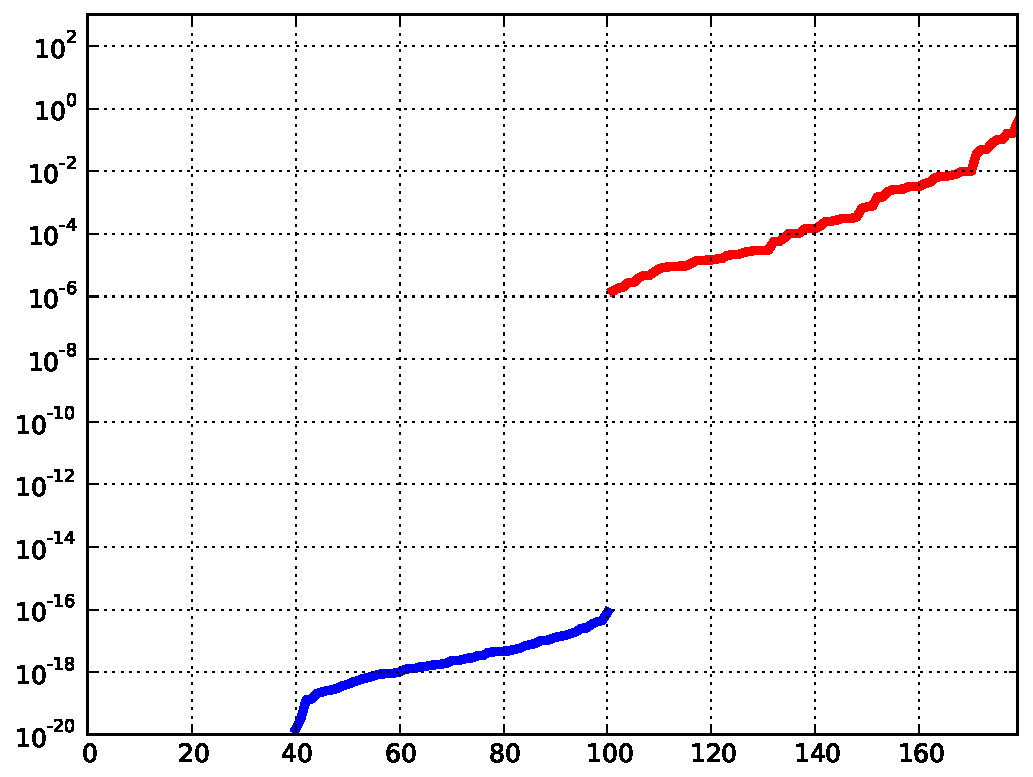
\includegraphics[width=4cm]{figs/shearlets/eigs/rid_dbl_nper_mass1}
& 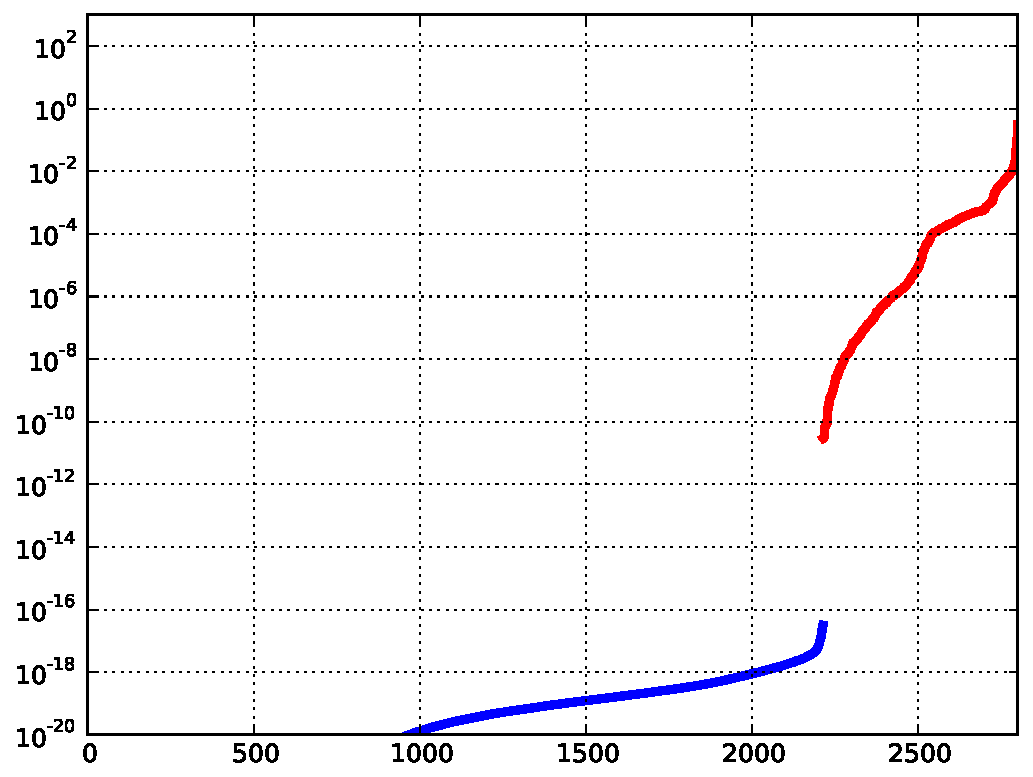
\includegraphics[width=4cm]{figs/shearlets/eigs/rid_dbl_nper_mass2} \\
\rotatebox{90}{\hspace{0.7cm}Transport}
& 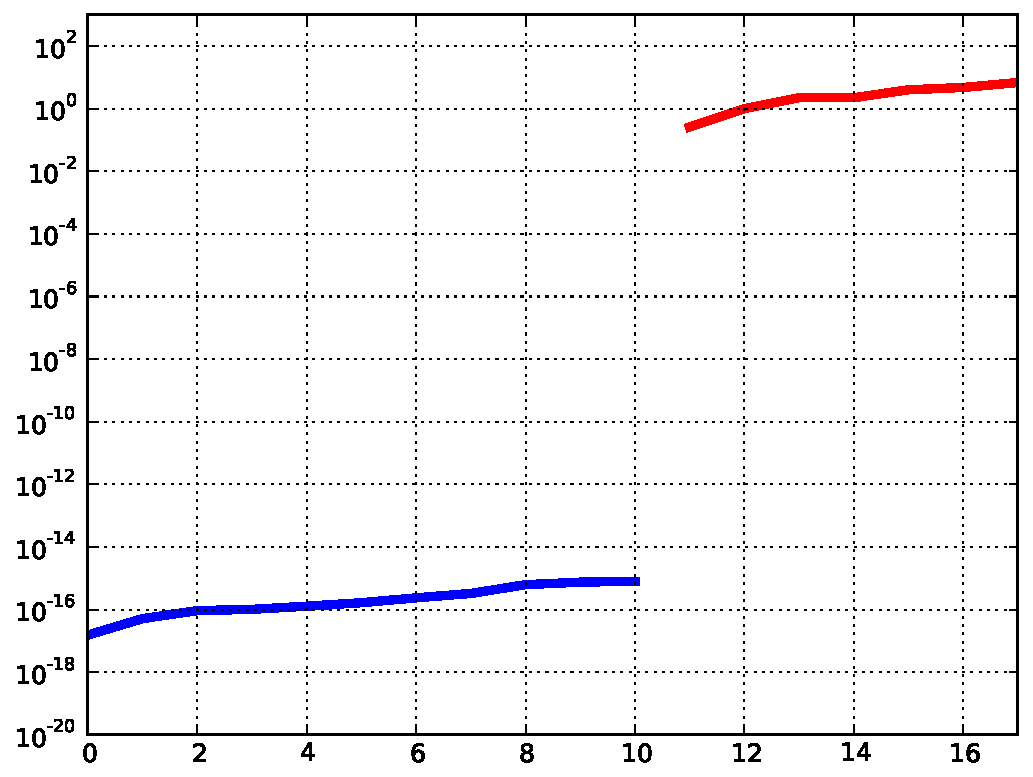
\includegraphics[width=4cm]{figs/shearlets/eigs/rid_dbl_nper_tran0}
& 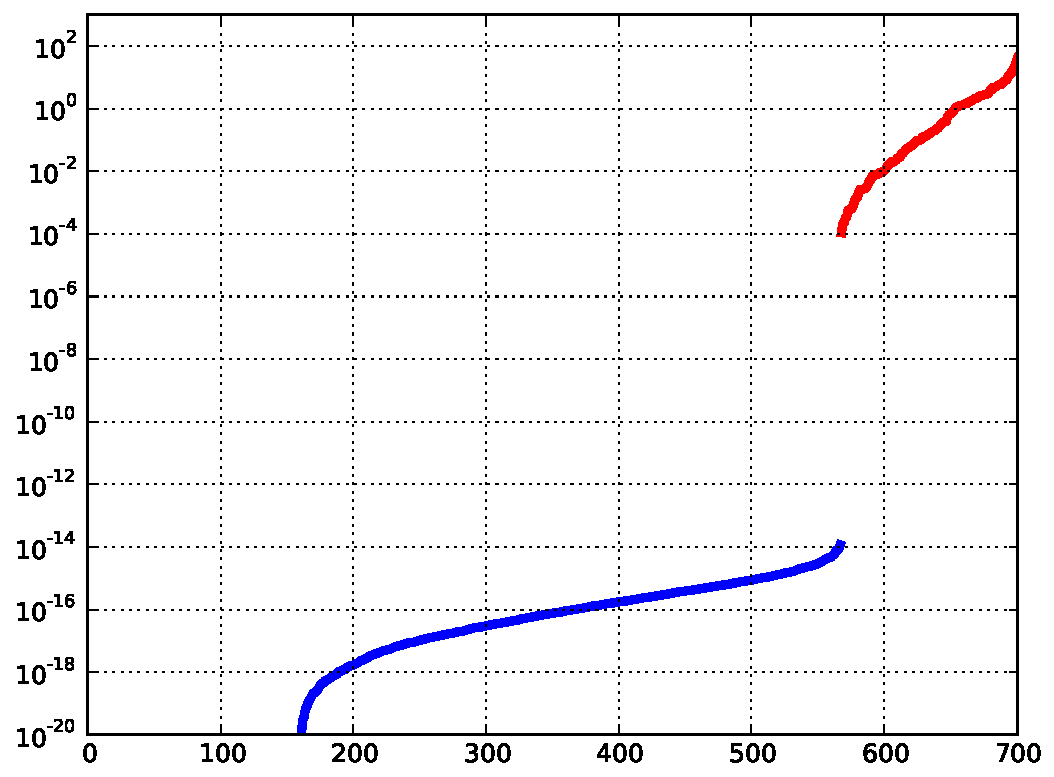
\includegraphics[width=4cm]{figs/shearlets/eigs/rid_dbl_nper_tran1}
& 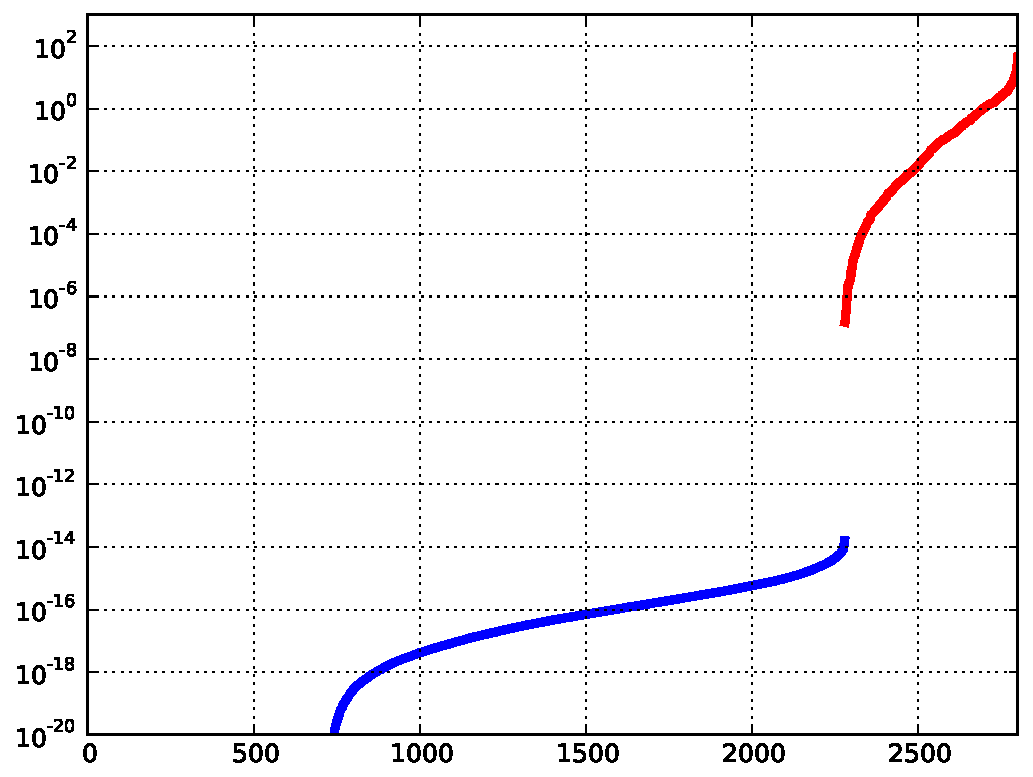
\includegraphics[width=4cm]{figs/shearlets/eigs/rid_dbl_nper_tran2}
\end{tabular}
\caption{Non-periodic, $(s_x,s_y)=(2,1)$.}
\label{fig:rid_dbl_nper}
\end{figure}

\begin{figure}
\hspace{-1.3cm}
\centering
\begin{tabular}{cccc}
& $j=0$ & $j=1$ & $j=2$ \\
\rotatebox{90}{\hspace{1.1cm}Mass} 
& 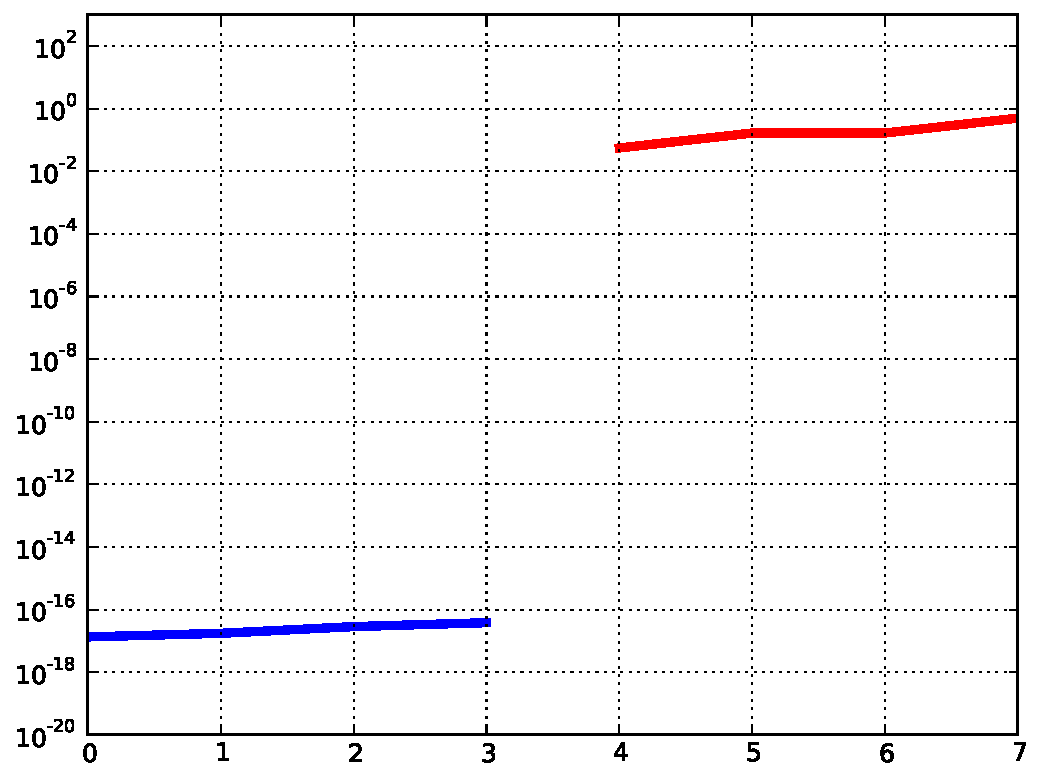
\includegraphics[width=4cm]{figs/shearlets/eigs/rid_dbl_per_mass0}
& 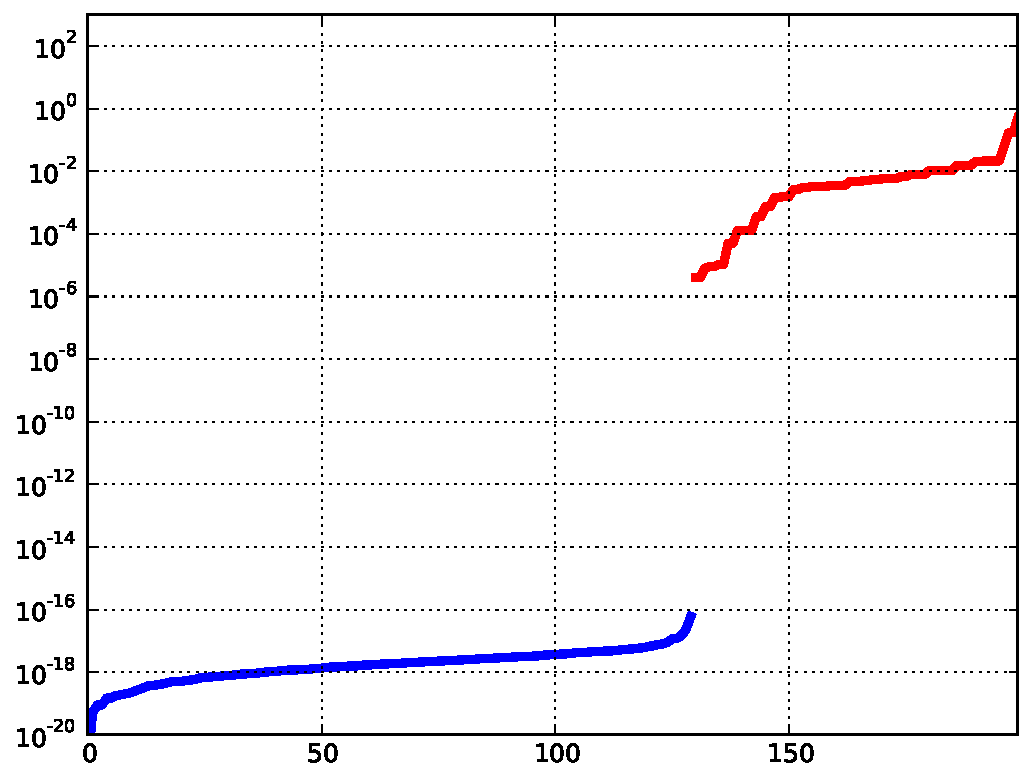
\includegraphics[width=4cm]{figs/shearlets/eigs/rid_dbl_per_mass1}
& 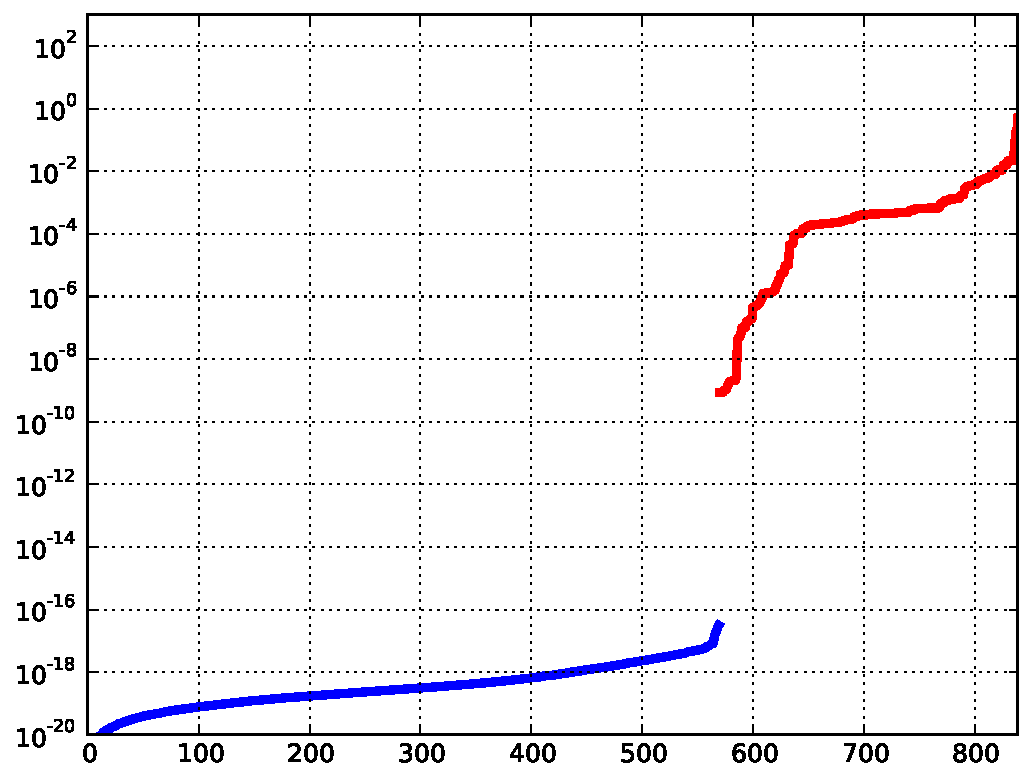
\includegraphics[width=4cm]{figs/shearlets/eigs/rid_dbl_per_mass2} \\
\rotatebox{90}{\hspace{0.7cm}Transport}
& 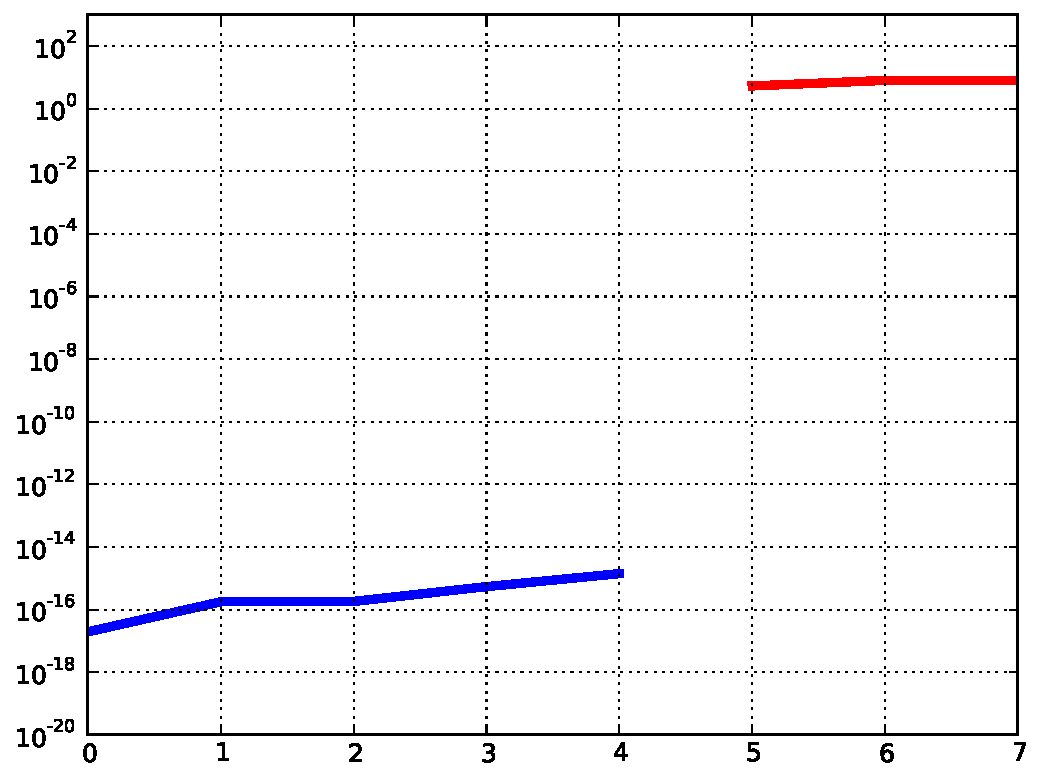
\includegraphics[width=4cm]{figs/shearlets/eigs/rid_dbl_per_tran0}
& 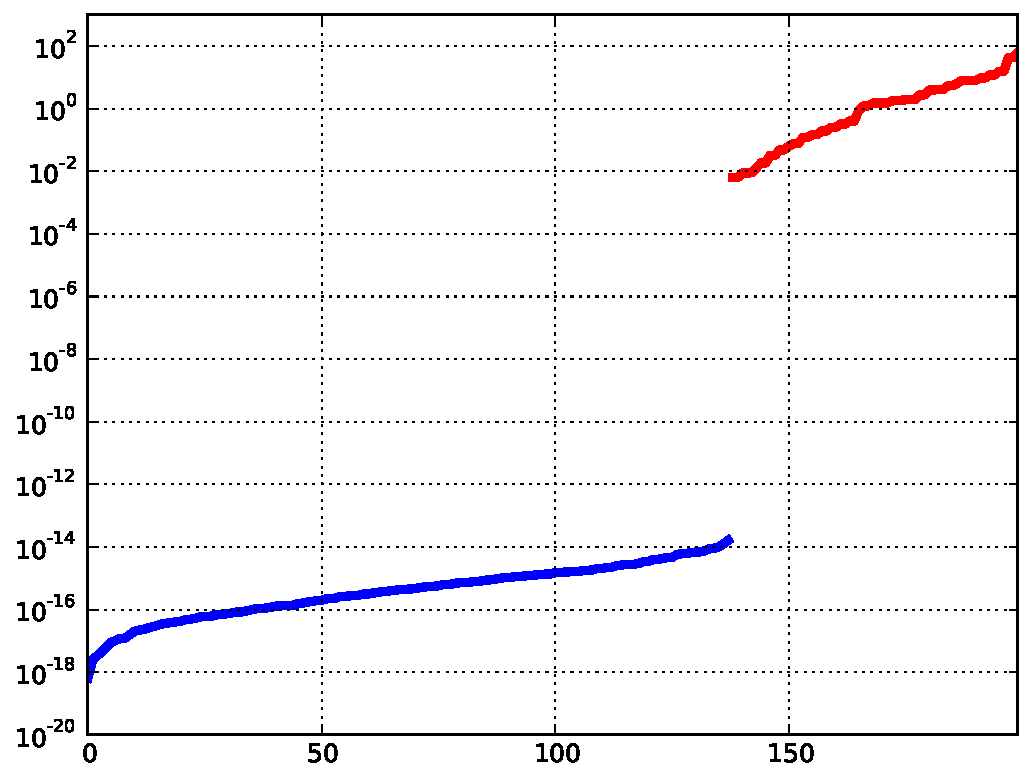
\includegraphics[width=4cm]{figs/shearlets/eigs/rid_dbl_per_tran1}
& 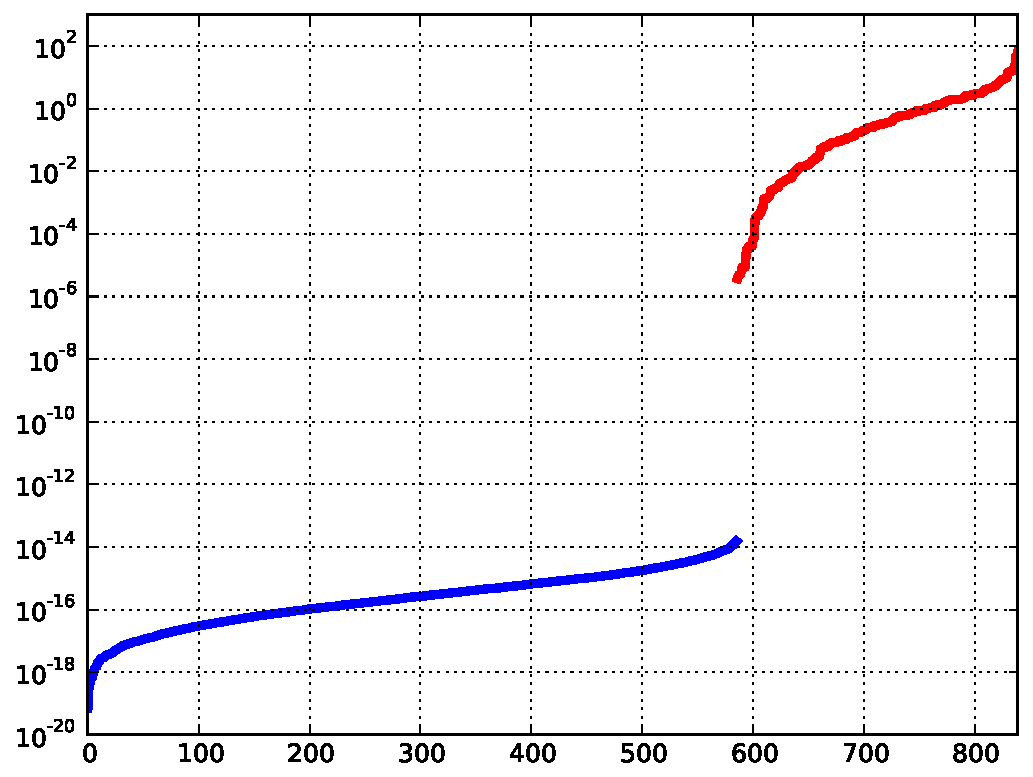
\includegraphics[width=4cm]{figs/shearlets/eigs/rid_dbl_per_tran2}
\end{tabular}
\caption{Periodic, $(s_x,s_y)=(2,1)$.}
\label{fig:rid_dbl_per}
\end{figure}

\begin{figure}
\hspace{-1.3cm}
\centering
\begin{tabular}{cccc}
& $j=0$ & $j=1$ & $j=2$ \\
\rotatebox{90}{\hspace{1.1cm}Mass} 
& 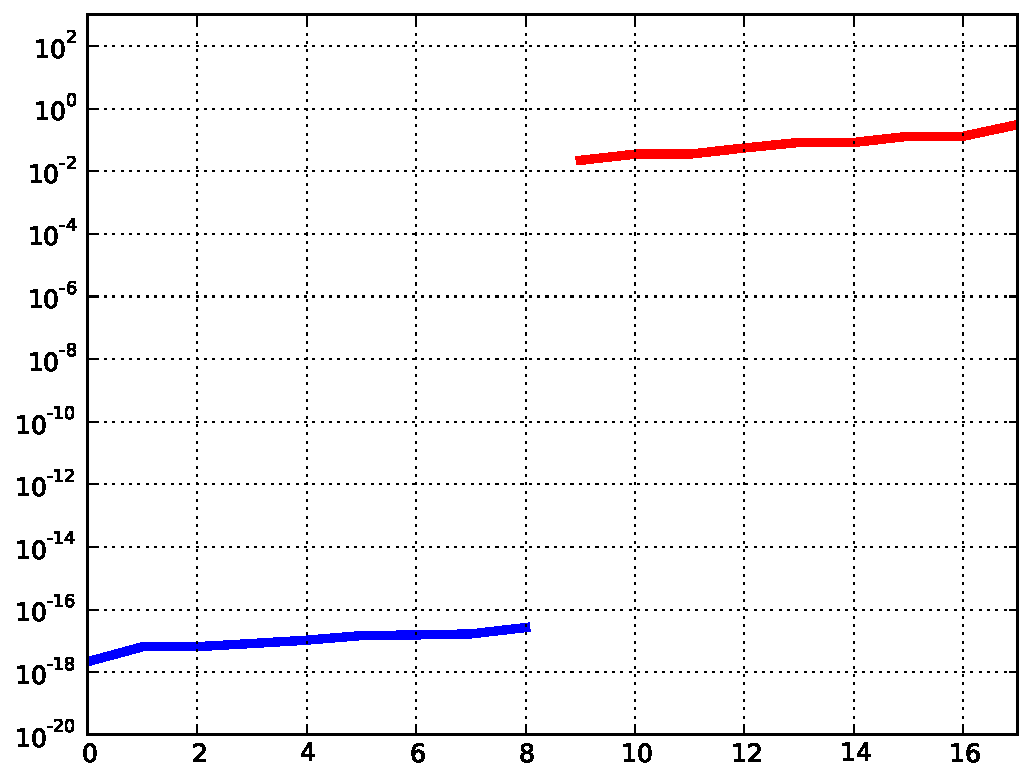
\includegraphics[width=4cm]{figs/shearlets/eigs/rid_sglhat_nper_mass0}
& 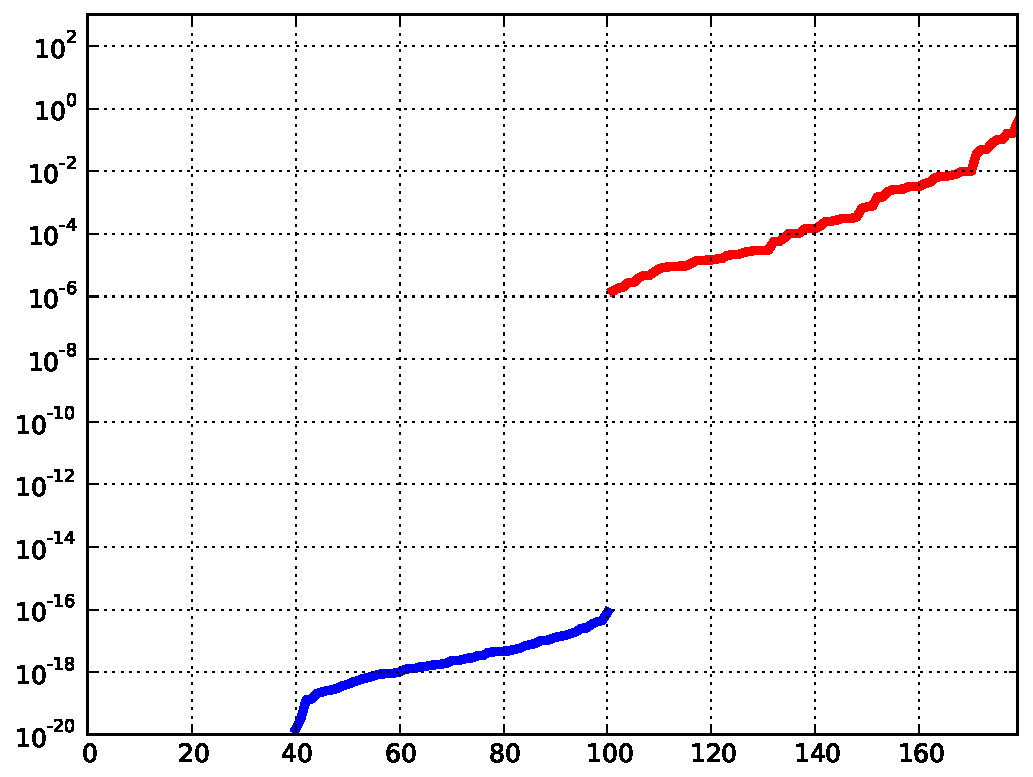
\includegraphics[width=4cm]{figs/shearlets/eigs/rid_sglhat_nper_mass1}
& 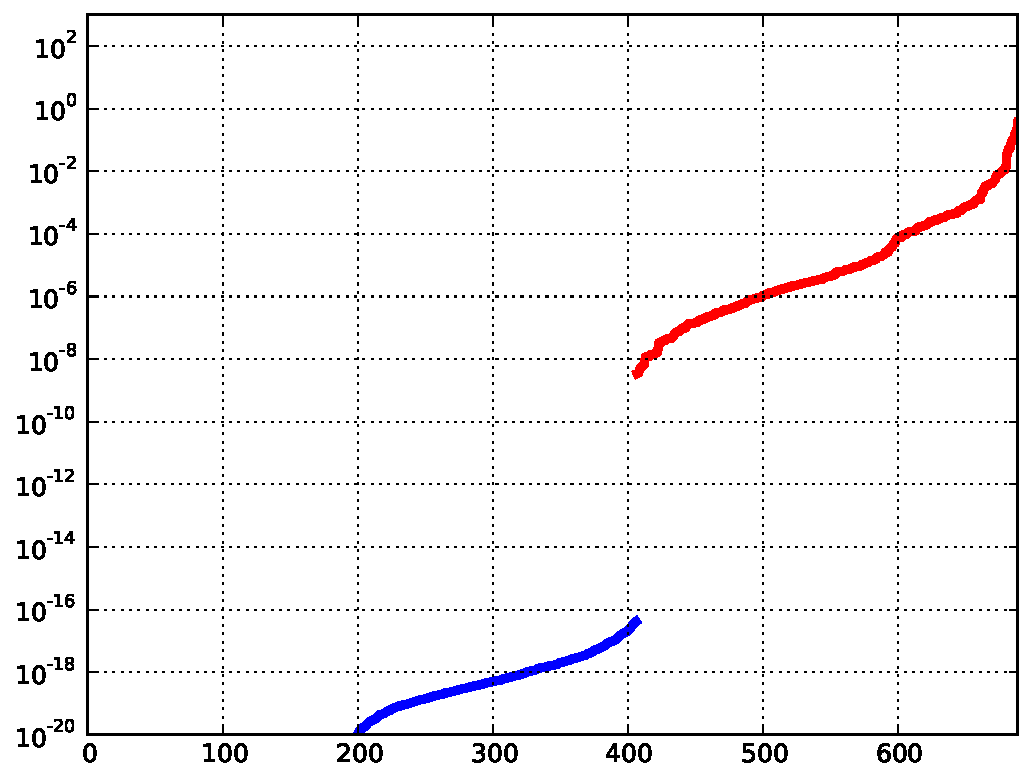
\includegraphics[width=4cm]{figs/shearlets/eigs/rid_sglhat_nper_mass2} \\
\rotatebox{90}{\hspace{0.7cm}Transport}
& 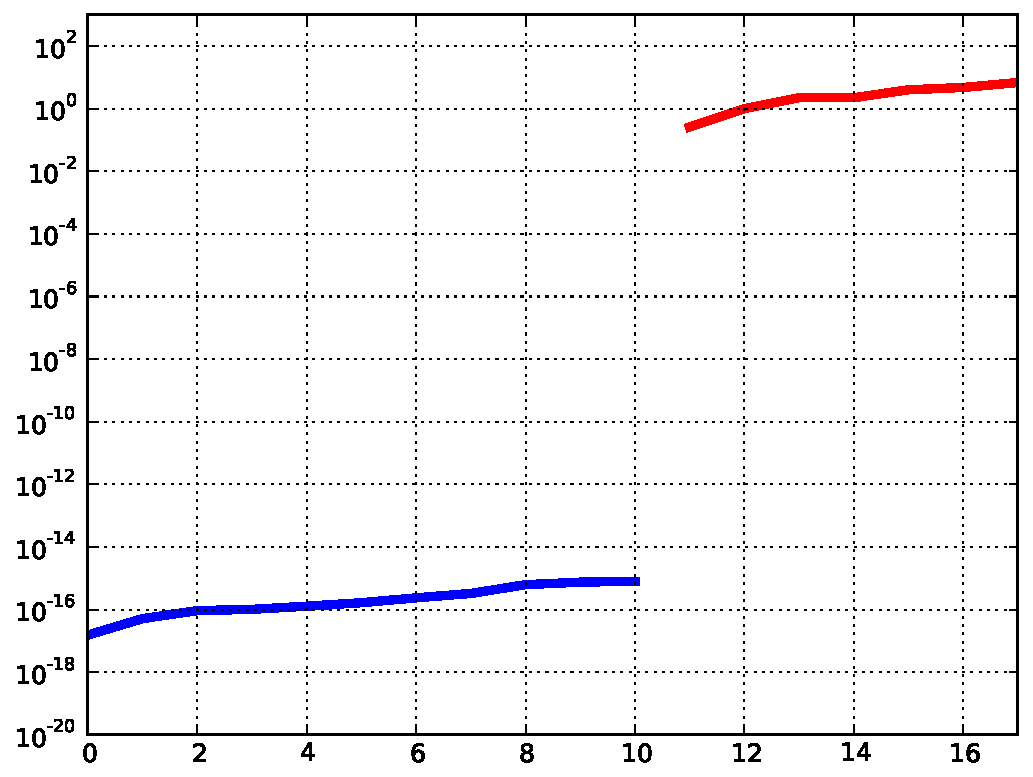
\includegraphics[width=4cm]{figs/shearlets/eigs/rid_sglhat_nper_tran0}
& 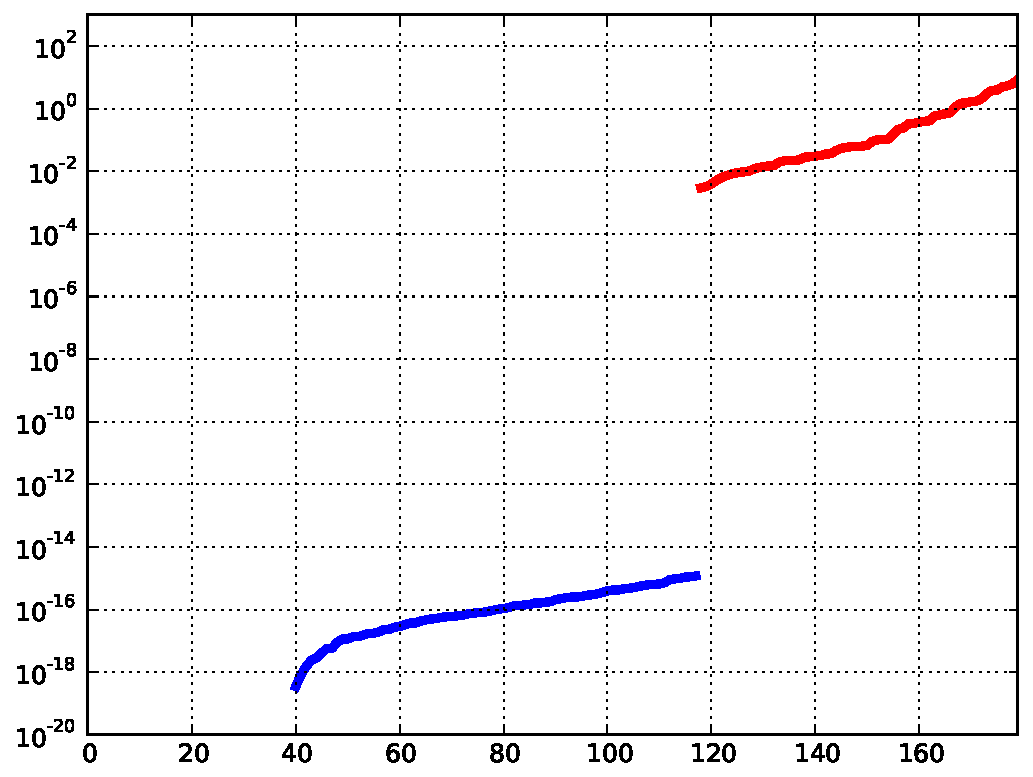
\includegraphics[width=4cm]{figs/shearlets/eigs/rid_sglhat_nper_tran1}
& 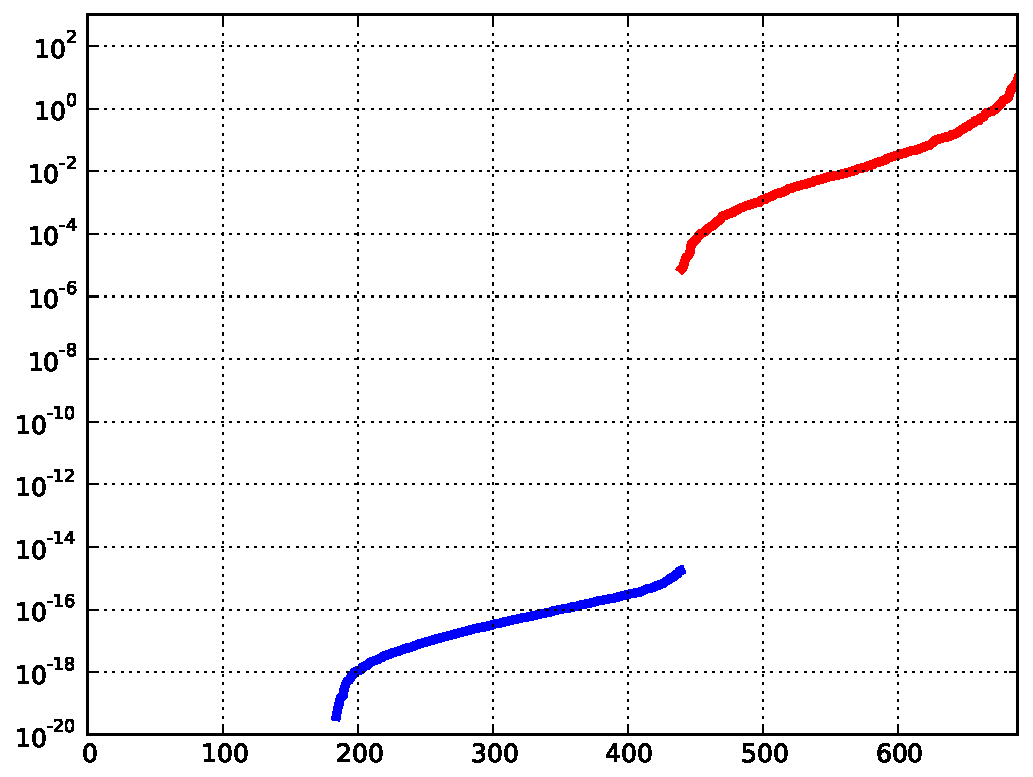
\includegraphics[width=4cm]{figs/shearlets/eigs/rid_sglhat_nper_tran2}
\end{tabular}
\caption{Non-periodic hat functions, $(s_x,s_y)=(2,1)$.}
\label{fig:rid_sglhat_nper}
\end{figure}

\begin{figure}
\hspace{-1.3cm}
\centering
\begin{tabular}{cccc}
& $j=0$ & $j=1$ & $j=2$ \\
\rotatebox{90}{\hspace{1.1cm}Mass} 
& 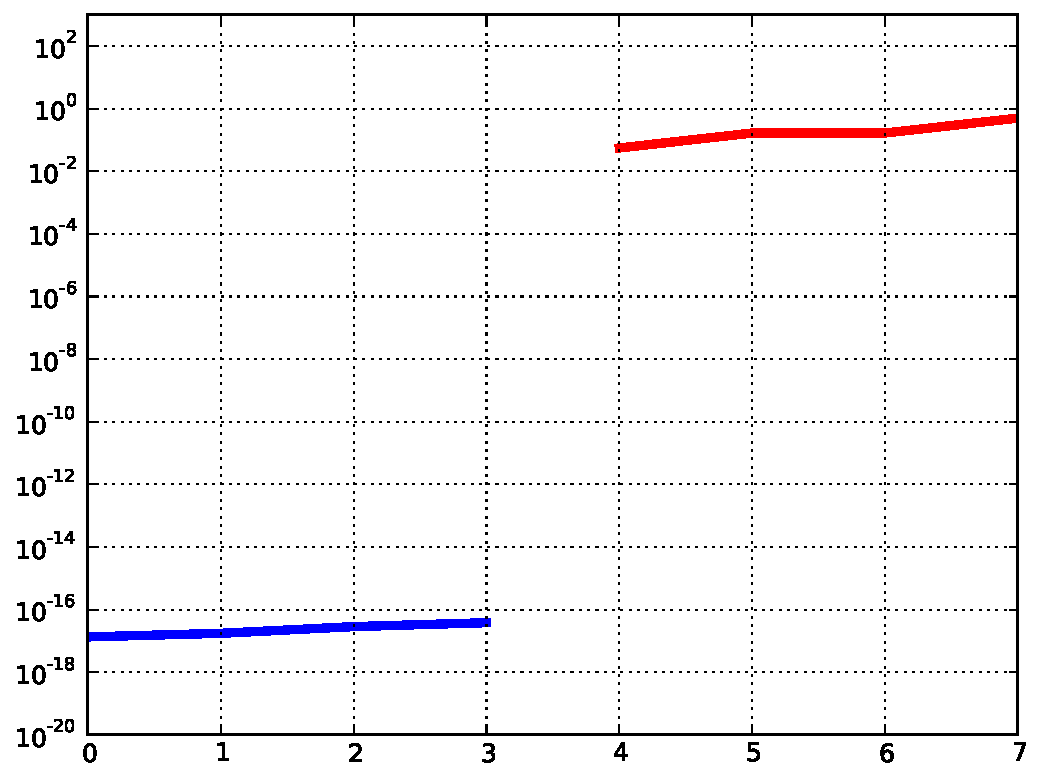
\includegraphics[width=4cm]{figs/shearlets/eigs/rid_sglhat_per_mass0}
& 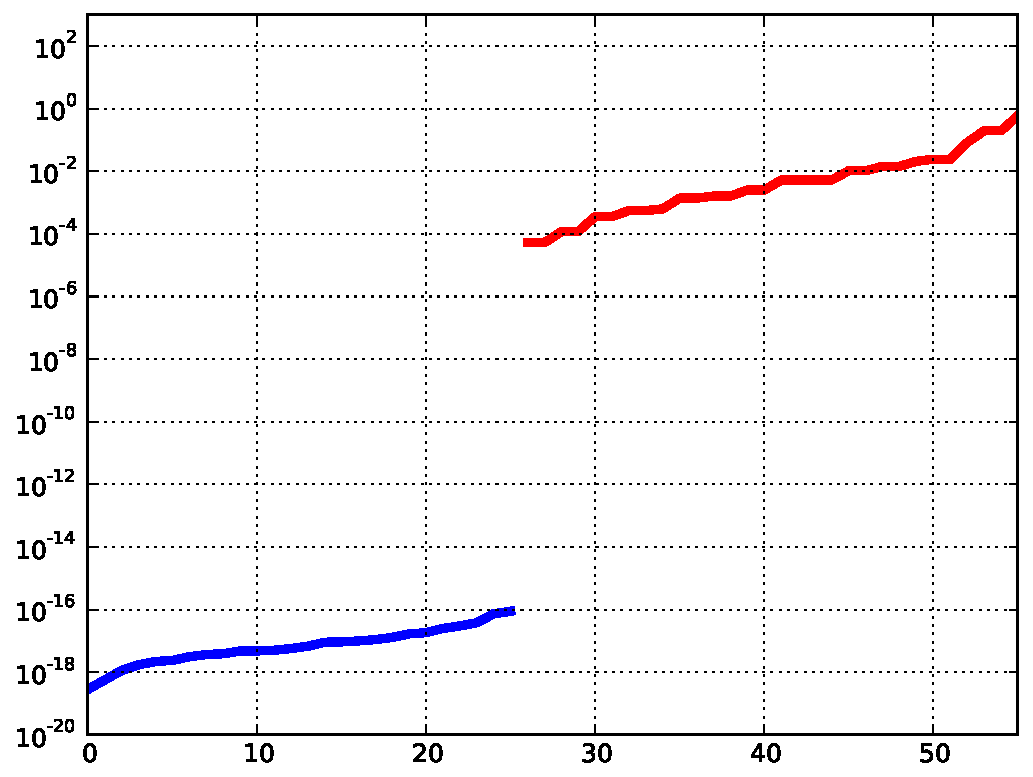
\includegraphics[width=4cm]{figs/shearlets/eigs/rid_sglhat_per_mass1}
& 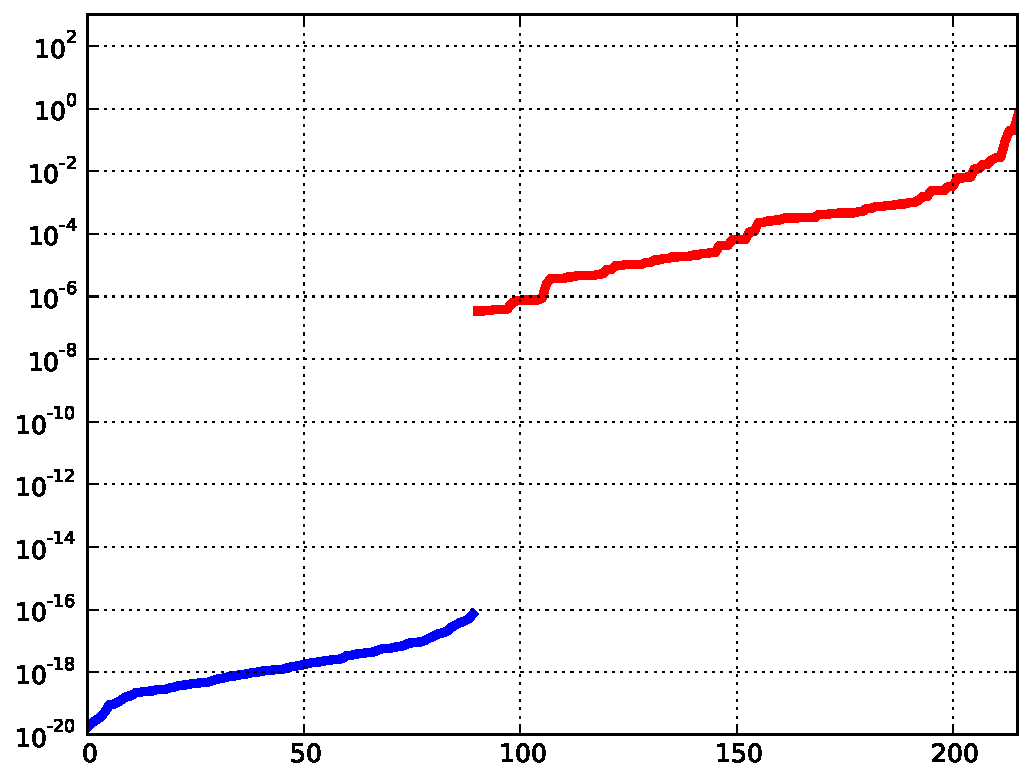
\includegraphics[width=4cm]{figs/shearlets/eigs/rid_sglhat_per_mass2} \\
\rotatebox{90}{\hspace{0.7cm}Transport}
& 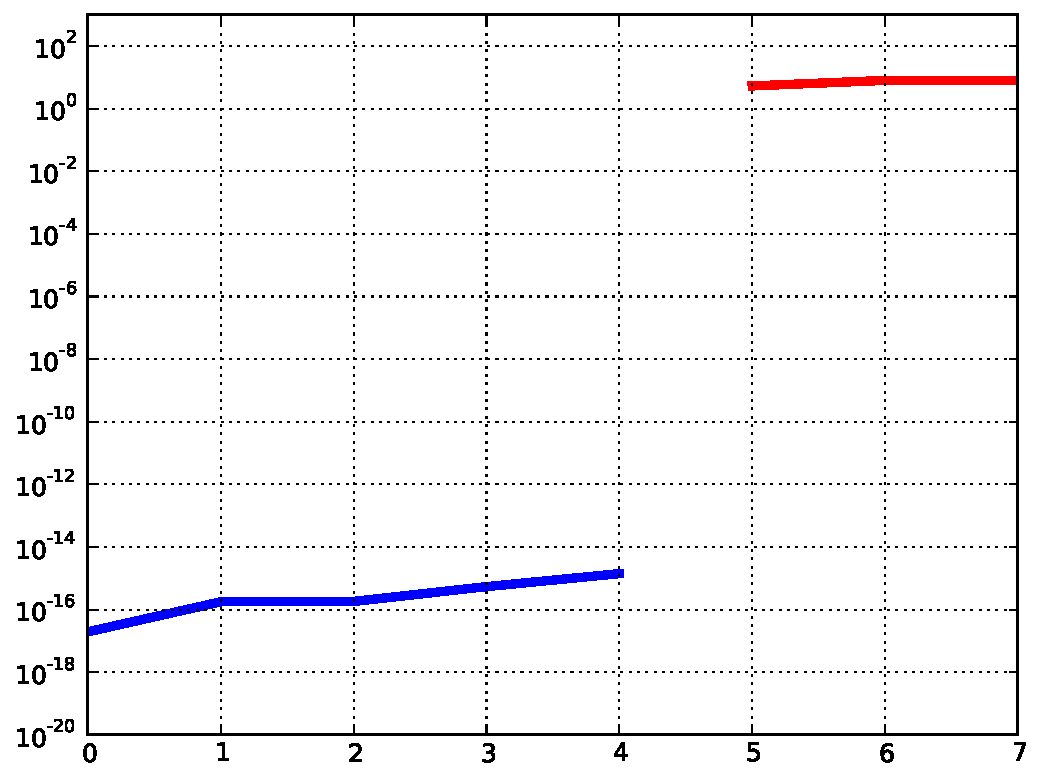
\includegraphics[width=4cm]{figs/shearlets/eigs/rid_sglhat_per_tran0}
& 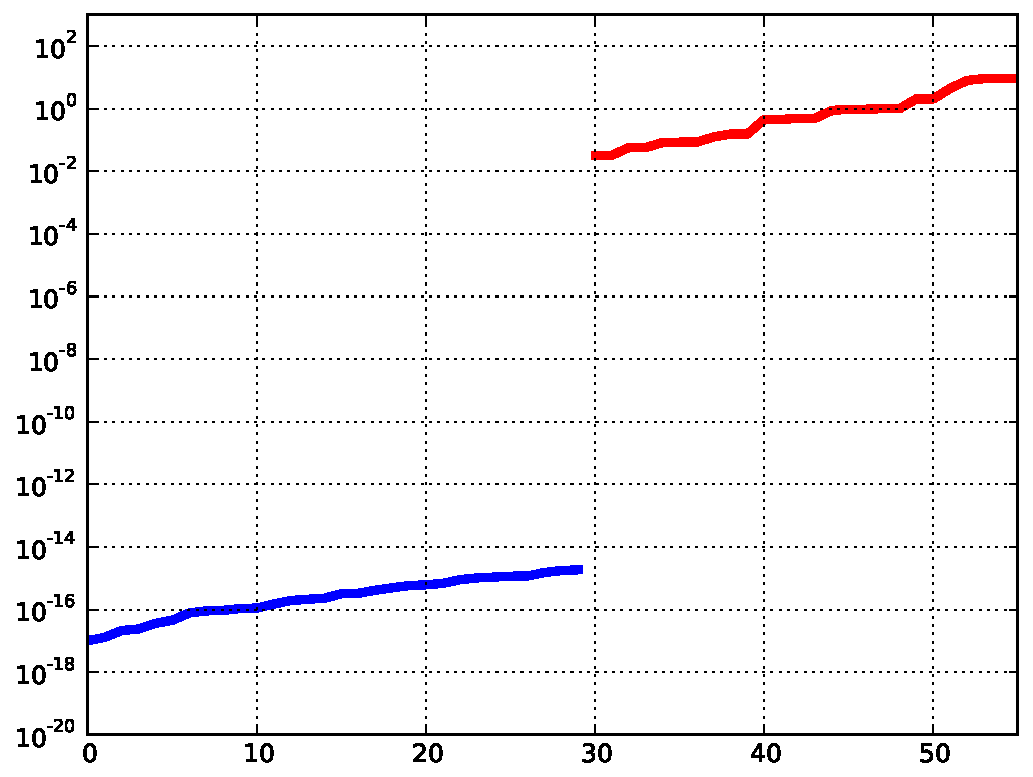
\includegraphics[width=4cm]{figs/shearlets/eigs/rid_sglhat_per_tran1}
& 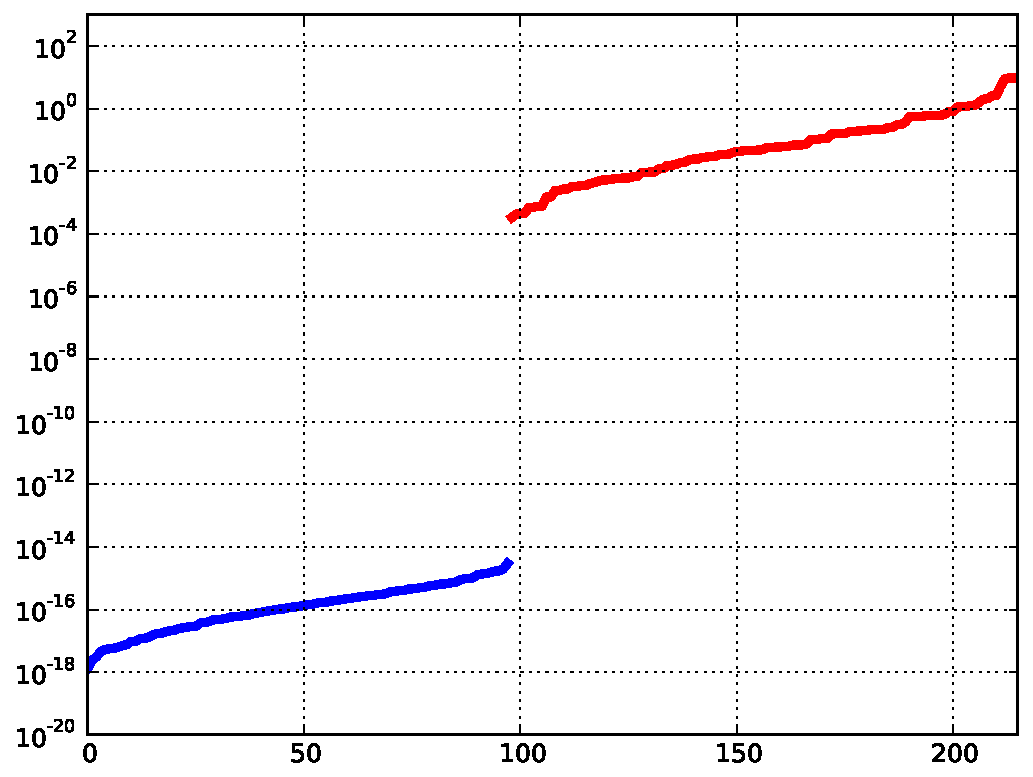
\includegraphics[width=4cm]{figs/shearlets/eigs/rid_sglhat_per_tran2}
\end{tabular}
\caption{Periodic hat functions, $(s_x,s_y)=(2,1)$.}
\label{fig:rid_sglhat_per}
\end{figure}

\begin{landscape}
\begin{table}
\centering
\def\arraystretch{1.2}
\begin{tabular}{ccccccccc}
$s_x$ & $s_y$ & Periodic & Mothers & Matrix & $j=0$ & $j=1$ & $j=2$ & $j=3$ \\
\hline \noalign{\vskip 1mm} 
$4$ & $2$ & No & Normal & Mass & $1.39\cdot10^1$ & $1.19\cdot10^9$ & & \\
\hline \noalign{\vskip 1mm}
$4$ & $2$ & No & Normal & Transport & $2.61\cdot10^1$ & $6.24\cdot10^6$ & & \\
\hline \noalign{\vskip 1mm}
$4$ & $2$ & Yes & Normal & Mass & $9.00\cdot10^0$ & $5.66\cdot10^7$ & & \\
\hline \noalign{\vskip 1mm}
$4$ & $2$ & Yes & Normal & Transport & $1.50\cdot10^0$ & $6.83\cdot10^5$ & & \\
\hline \noalign{\vskip 1mm} 
$2$ & $1$ & No & Normal & Mass & $1.39\cdot10^1$ & $2.51\cdot10^5$ & $1.05\cdot10^{10}$ & \\
\hline \noalign{\vskip 1mm}
$2$ & $1$ & No & Normal & Transport & $2.61\cdot10^1$ & $3.99\cdot10^5$ & $3.02\cdot10^8$ & \\
\hline \noalign{\vskip 1mm}
$2$ & $1$ & Yes & Normal & Mass & $9.00\cdot10^0$ & $1.23\cdot10^5$ & $5.73\cdot10^8$ & \\
\hline \noalign{\vskip 1mm}
$2$ & $1$ & Yes & Normal & Transport & $1.50\cdot10^0$ & $1.02\cdot10^4$ & $1.79\cdot10^7$ & \\
\hline \noalign{\vskip 1mm} 
$2$ & $1$ & No & Single & Mass & $1.39\cdot10^1$ & $2.51\cdot10^5$ & $1.10\cdot10^8$ & $2.61\cdot10^{11}$ \\
\hline \noalign{\vskip 1mm}
$2$ & $1$ & No & Single & Transport & $2.61\cdot10^1$ & $2.92\cdot10^3$ & $1.15\cdot10^6$ & $6.76\cdot10^8$ \\
\hline \noalign{\vskip 1mm}
$2$ & $1$ & Yes & Single & Mass & $9.00\cdot10^0$ & $1.13\cdot10^4$ & $1.78\cdot10^6$ & $6.76\cdot10^8$ \\
\hline \noalign{\vskip 1mm}
$2$ & $1$ & Yes & Single & Transport & $1.50\cdot10^0$ & $2.87\cdot10^2$ & $2.88\cdot10^4$ & $7.41\cdot10^6$ \\
\end{tabular}
\caption{Effective condition numbers for all cases shown in Figure \ref{fig:shl_dbl_nper} through
\ref{fig:rid_sglhat_per}.}
\label{tbl:shletconds}
\end{table}
\end{landscape}

\cleardoublepage

\chapter{Homogeneous Boltzmann equation: sparse Fourier spectral scheme}
\chaptermark{HBE: sparse Fourier spectral scheme}
\label{chap:boltzmann-fourier}

\section{Introduction} 
\label{sect:boltzmann}

For the remainder of this dissertation, we will focus on the spatially homogeneous Boltzmann equation,
\begin{equation} \label{eqn:boltzmann-sphom}
    \frac{\partial f}{\partial t} = Q(f,f),
\end{equation}
where $Q$ is the Boltzmann collision operator introduced in Section~\ref{sec:boltzmann-intro}.

The most popular methods for the solution of \eqref{eqn:boltzmann-sphom} are stochastic Monte Carlo-type
methods. Determenistic schemes do not suffer from problems of indeterminism, noise and slow convergence, but
they are generally very expensive. Lattice Boltzmann methods, which rely on very crude pointwise
discretizations in velocity space have also become popular. Since our work is primarily concerned with
high-accuracy spectral determenistic methods, no attempt will be made in the following to compare our work
with stochastic methods or lattice Boltzmann methods.

Existing work on the discretization of \eqref{eqn:boltzmann-sphom} rely heavily on Fourier spectral
discretization, which can exploit the convolution structure of $Q$ owing to the translation invariance of
Theorem~\ref{thm:trans-rot-Q}. See \cite{Bobylev88, Kirsch07, Pareschi96} and \cite{Gamba09, Gamba10,
Filbet06, Pareschi00, Pareschi03} for numerical simulations based on that method. Also related to this are the
difference methods developed in \cite{BobylevR97, Bobylev99, Bobylev00} and \cite{Ibragimov02}.

The approach entails two fundamental modifications of the collision operator:
\begin{enumerate}
  \renewcommand{\labelenumi}{(\roman{enumi})}
  \item the restriction of the integration over $\bbR^{d}$ in~(\ref{eqn:Q-std}) to 
    a ball of finite radius $R>0$, see Section~\ref{sec:trunc} for details, 
  \item the truncation of the velocity space $\bbR^{d}$ to a cube $\cD_{L} := [-L,L)^{d}$ plus
    periodic continuation. 
\end{enumerate}
These result in a perturbed evolution
\begin{gather}
  \label{eqn:QR}
  \frac{\partial}{\partial t}{f}_R = Q^R(f_R, f_R), \qquad f(0) = f_0.
\end{gather}
Clearly, its solution depends on both $R$ and $L$. The exact definition of $Q^R$ will be given in
Section~\ref{sec:fourier}.

Subsequently, \eqref{eqn:QR} is projected onto a subspace of $L^{2}(\cD_{L})$ spanned by a
finite set of Fourier modes. An in-depth analysis of the discretization error due
to this last step has recently been developed by Filbet and Mouhot in \cite{Filbet11},
and in parts of our work we are going to rely on their techniques. 

One of our main goals was to provide a priori estimates of the discretization error for \eqref{eqn:QR} in
$H^{s}$-Sobolev norms, $s\geq 0$, for rather general sets of Fourier modes, which includes as a special cases
the so-called hyperbolic crosses. For certain types of solutions, this scheme offers much more efficient
approximation compared to the full tensor product space of Fourier modes. This extends the results of
\cite{Filbet11}. 

In another respect we go beyond \cite{Filbet11}: we also quantify the impact of
switching from (\ref{eqn:boltzmann-sphom}) to (\ref{eqn:QR}), conditional
on the following conjecture.
\begin{conjecture} \label{ass:decay}
  For given Sobolev index $s\geq 0$, assume that there exist $C_0>0$ and $a>0$ so that the solution
  $f_R$ of \eqref{eqn:QR} fulfills
  $$
  |\partial^\Balpha f_R(t,\Bv)| \le C_0\exp\left(-a|\Bv|^2\right),
  $$
  and that there exists a polynomial $\Pi(L)$ so that
  $$
  \| \exp\left(a|\Bv|^2\right) \partial^\Balpha f_R(t,\Bv) \|_{L^2(\cD_L)} \leq
  \Pi(L),
  $$
  for all $|\Balpha|_1\leq s$, $t\geq0$ and $f_{R}$ solving (\ref{eqn:QR}).
\end{conjecture}
\begin{remark}
  The decay condition on $f_R$ is formulated in this form since it is
  $2L$-periodic, and thus it cannot satisfy any classical decay condition on the
  whole of $\bbR^d$. The polynomial dependence on $L$ is allowed so that 
  equilibrium solutions fit the assumption. For example, if $\Balpha=0$ and 
  $f_R(t,\Bv)=\exp(-a|\Bv|^2)$ we require $\Pi(L) \geq (2L)^{\nicefrac{d}{2}}$.
  
  The decay of $f$ is well known, see for example \cite{Bobylev97}.  Yet, so far,
  there is no rigorous proof that the Conjecture~\ref{ass:decay} holds for
  $f_R$. We have only numerical evidence that this is true, see
  Section~\ref{sec:decay}.
\end{remark}

\textbf{Outline.} The chapter is structured as follows. In Section \ref{sec:fourier}
we develop the details of the truncation of $Q$ and the Fourier spectral discretization.
The following Section~\ref{sec:hyper} introduces the concrete Fourier spectral 
Galerkin discretization of (\ref{eqn:QR}) for families of hyperbolic cross Fourier
modes. In Section~\ref{sec:appr} we develop the main a priori convergence
estimates, which are summarized in Theorem~\ref{thm:mainapprox} (consistency
estimates), Theorem~\ref{thm:discrerror} (Fourier spectral discretization error
for (\ref{eqn:QR})), and Proposition~\ref{prop:err-R} (estimate for $f-f_{R}$). 
We emphasize that Conjecture~\ref{ass:decay} is essential only for this last result.

Numerical experiments for all Fourier-based methods discussed are reported in Section~\ref{sec:numerical-fou}.
They highlight the conditions that have to met for satisfactory performance of the hyperbolic cross
approximation.  They also convey the importance of choosing a sufficiently small ratio $R:L$ in order to avoid
aliasing.

\section[Fourier discretization of the Boltzmann collision operator]{Fourier discretization of the Boltzmann collision operator%
    \sectionmark{Fourier discr. of the Boltzmann collision operator}}
\sectionmark{Fourier discr. of the Boltzmann collision operator}
\label{sec:fourier}

In this section we aim to discretize the solution $f$ by a finite Fourier
series. Of course, integrals such as \eqref{eqn:Q-p} and \eqref{eqn:Q-m} will
diverge for periodic $f$. Thus, a truncation in velocity is required.

\subsection{Truncation in velocity space} \label{sec:trunc}

In this section, we develop equivalent {\em truncated} forms for the collision
operator as defined via
\begin{equation} \label{eqn:Q-p}
    Q(f,h)(\Bv) = \int_{\bbR^d}\int_{\bbS^{d-1}} B(|\Bg|,\cos\theta)(h_*'f' -
    h(\Bv-\Bg)f(\Bv))\dd\Bsigma \dd \Bg,
\end{equation}
which is achieved through a change of variables $\Bg=\Bv-\Bv_*$, and the {\em
Carleman representation}
\begin{multline} \label{eqn:Q-m}
    Q(f,h)(\Bv) = \int_{\bbR^d}\int_{\bbR^d} \Bt(\Bx,\By) \delta(\Bx\cdot\By) \\
    \left[ h(\Bv+\By)f(\Bv+\Bx) - h(\Bv+\Bx+\By)f(\Bv) \right] \dd \Bx \dd \By,
\end{multline}
whose derivation is detailed in \cite{Mouhot06} and also in \cite{Bobylev99} for hard sphere collision
kernels ($B\equiv|\Bg|$).

The following proposition is given in \cite{Pareschi00}, with $\B_R$ denoting
the ball of radius $R$ centered at $0$. It follows more or less straightforwardly from \cite{Pareschi96}.
\begin{proposition}[Proposition 3.1 in \cite{Pareschi00}] \label{prop:trunc}
Let $\supp f,h\subseteq\B_R$. Then, $\supp Q(f,h)\subseteq\Bsr$, and 
\[ 
    Q(f,h)(\Bv) = \int_{\Btr}\int_{\bbS^{d-1}} 
            B(|\Bg|,\cos\theta)(h_*'f'-h_*f)\dd\Bsigma \dd \Bg 
\]
for $\Bv\in\Bsr$. Under these assumptions,
$\Bv',\Bv_*',\Bv-\Bg\in\B_{(2+\sqrt{2})R}$ for all $\Bg\in\Btr$.
\end{proposition}
Thus, by considering $f$ restricted on the cube $\cD_L=[-L,L]^d$, with
$f(\Bv)=0$ on $\cD_L\setminus\B_R$, extended periodically to all of $\bbR^d$, we
can evaluate $Q(f,f)$ without aliasing if $\nicefrac{R}{L}$ is small enough. In
practice, $L$ should be chosen large enough to accommodate the necessary number
of timesteps while minimizing the aliasing errors, as the support of $f$ will
grow.

Common practice \cite{Pareschi00, Mouhot06} is to choose $R,L$ so that aliasing is avoided for one
single application of the collision operator. This holds if
$$
    \kappa = \frac{R}{L} \leq \frac{2}{3+\sqrt{2}},
$$
see for example \cite[Fig. 1]{Pareschi00}.  In Section~\ref{sec:aliasing} we present some numerical
experiments showing how the choice of $\kappa$ can significantly impact the performance of a numerical scheme.

The task is now to bring the Carleman representation \eqref{eqn:Q-m} into
truncated form also, so that the two truncated representations are equivalent.
This is the content of the following proposition.

\begin{proposition} \label{prop:equiv}
Consider $f$ and $h$ restricted to the cube $\cD_L$ with $f(\Bv)=0$ on
$\cD_L\setminus\B_R$, extended periodically to all of $\bbR^d$, with
$\kappa=\nicefrac{R}{L}\leq\nicefrac{2}{(3+\sqrt{2})}$. Then, for $v\in\Bsr$, the
following representations of $Q(f,h)(\Bv)$ agree.
\begin{align}
    \label{eqn:Q-p-b}
    Q^R_{\mathrm{P}}(f,h) &\defeq 
    \int_{\Btr}\int_{\bbS^{d-1}} B(|\Bg|,\theta)(h_*'f'-h_*f)\dd\Bsigma \dd \Bg \\
    \label{eqn:Q-m-b} 
    Q^R_{\mathrm{M}}(f,h) &\defeq \int_{\Bsr}\int_{\Bsr} \Bt(\Bx,\By)\delta(\Bx\cdot \By) \\
    \nonumber & \qquad\qquad\qquad\qquad
        \left[ h(\Bv+\By)f(\Bv+\Bx) - h(\Bv+\Bx+\By)f(\Bv) \right] \dd \Bx \dd \By
\end{align}
\end{proposition}
\begin{proof}
Representation \eqref{eqn:Q-p-b} follows from Proposition \ref{prop:trunc}.
Following the policy from \cite{Mouhot06}, it can be shown that 
\begin{multline*}
    Q(f,h)(\Bv) = \int_{\bbR^d}\int_{\bbR^d}\Bt(\Bx,\By)\delta(\Bx\cdot \By)\chi_{\B_{2R}}(\Bx+\By)  \\ 
    \left[h(\Bv+\By)f(\Bv+\Bx)-h(\Bv+\Bx+\By)f(\Bv)\right] \dd \Bx \dd \By. 
\end{multline*}
It remains to show that when $|\Bx+\By|>2R$, i.e. when
$\chi_{\Btr}(\Bx+\By)=0$, we have $h(\Bv+\By)f(\Bv+\Bx) = h(\Bv+\Bx+\By)f(\Bv)
= 0$.

Under these assumptions, it is clear that either $|\Bv|>R$ or
$|\Bv+\Bx+\By|>R$. Furthermore, since $\Bx\perp \By$, we also have
$|\Bx-\By|>2R$, so either $|\Bv+\By|>R$ or $|\Bv+\Bx| =
|(\Bv+\By)+(\Bx-\By)| > R$.

Last, for $|\Bx|,|\By|\leq\sqrt{2}R$, we have
\[
    \max\{|\Bv|,|\Bv+\Bx|,|\Bv+\By|,|\Bv+\Bx+\By|\} \leq 2L-R,
\]
so aliasing is avoided. This concludes the proof.
\end{proof}

Henceforth, we will denote by $Q^R$ the truncated version of $Q$ as defined in \eqref{eqn:Q-p-b} and
\eqref{eqn:Q-m-b}. We will also denote by $Q^{R,+}$ and $Q^{R,-}$ the corresponding truncated versions of
$Q^+$ and $Q^-$. We will always assume that the ratio of $R$ and $L$ is fixed and denote it by the constant
truncation parameter $\kappa=\nicefrac{R}{L}$.

\subsection{Fourier discretization} \label{sec:FourierDiscretization}

Following ideas from \cite{Gottlieb77, Canuto88}, let us now discretize $f$ by
representing it as a truncated $d$-dimensional Fourier series in $\Bv$, 
\begin{equation} \label{eqn:fn}
    f_\cA(t,\Bv) = \sum_{\Bk\in\cA} \hf_\Bk(t) \ee^{\ii\Bk\cdot\Bv},
\end{equation}
where $\cA\subset(\nicefrac{\pi}{L})\bbZ^d$ is some discrete and finite but so far
unspecified set of Fourier modes. Then, \eqref{eqn:boltzmann-sphom} yields
\begin{equation} \label{eqn:boltzmann-d-1}
    \sum_{\Bk\in\cA} \frac{\dd \hf_\Bk}{\dd t} \ee^{\ii\Bk\cdot \Bv} = \sum_{\Bl,\Bm\in\cA}
            \hf_\Bl\hf_\Bm Q^R\left(\ee^{\ii\Bl\cdot \Bv},
            \ee^{\ii\Bm\cdot \Bv}\right).
\end{equation}
Substituting the Fourier modes into \eqref{eqn:Q-p} or \eqref{eqn:Q-m}, we find
that there exist coefficients $\hbeta(\Bl,\Bm)$ so that
\begin{equation} \label{eqn:kmodes}
    Q^R\left(\ee^{\ii\Bl\cdot \Bv},\ee^{\ii\Bm\cdot \Bv}\right) = 
            \hbeta(\Bl,\Bm)\ee^{\ii(\Bm+\Bl)\cdot \Bv}
\end{equation}
for all $\Bl,\Bm \in (\nicefrac{\pi}{L})\bbZ^d$. This follows easily from a straightforward generalization of
Theorem~\ref{thm:trans-rot-Q}, since the transformation $\Bv \mapsto \Bv-\Bc$ leaves $\Bg$ and $\Bsigma$
unchanged. Equation \eqref{eqn:kmodes} is in many ways {\em raison d'\^{e}tre} for the whole method---the
justification for our transgressions in truncating $Q$.

Plugging this into \eqref{eqn:boltzmann-d-1}, discarding coefficients outside
$\cA$ and comparing the remaining coefficients, gives us the following quadratic
ordinary differential equation (ODE) for the coefficients $\hf_\Bk$:
\begin{equation} \label{eqn:boltzmann-d}
    \frac{\dd \hf_\Bk}{\dd t} = \sum_{\substack{\Bl,\Bm\in\cA \\
    \Bl+\Bm=\Bk}} \hf_\Bl\hf_\Bm\hbeta(\Bl,\Bm),\quad \Bk\in \cA.
\end{equation}
This is the Fourier space equivalent to seeking $f_\cA \in \spann \{ \ee^{\ii\Bl\cdot\Bv} \;:\; \Bl\in\cA \}$
so that
\begin{equation} \label{eqn:boltzmann-nd}
  \frac{\partial}{\partial t} {f}_\cA = P_\cA Q^R(f_\cA,f_\cA)
\end{equation}
where $P_\cA$ is the $L^2$-orthogonal projection on the the space spanned by the Fourier modes in $\cA$.

The coefficients $\hbeta(\Bl,\Bm)$ are called the {\em kernel modes}. These can be
evaluated through \eqref{eqn:kmodes}.  Note that since the Fourier modes
$\ee^{\ii\Bk\cdot \Bv}$ do not satisfy the conditions of Proposition
\ref{prop:equiv}, representations \eqref{eqn:Q-p-b} and \eqref{eqn:Q-m-b} will
yield {\em different} values for $\hbeta$. In the following, we will denote by
$\hbeta_d^\rmP$ those values arising from \eqref{eqn:Q-p-b}, and by $\hbeta_d^\rmM$ those
arising from \eqref{eqn:Q-m-b}. 

Separating gain and loss terms as described in Section~\ref{sect:boltzmann}, we
find that we have 
\[ 
    \hbeta_d^\ast(\Bl,\Bm) = \beta_d^\ast(\Bl,\Bm) - \beta_d^\ast(\Bm,\Bm),\qquad
    \ast \in \{\rmP,\rmM\}
\]
where the coefficients $\beta_d^\ast$ are given, for general kernels $B$ and $\Bt$, as 
\begin{multline} \label{eqn:B-p} 
    \beta_d^\rmP(\Bl,\Bm) = \int_{\Btr}\int_{\bbS^{d-1}} B(|\Bg|,\cos\theta) \\
    \exp\left[ -\ii\Bg\cdot\frac{\Bl+\Bm}{2} - 
        \ii|\Bg|\Bsigma\cdot\frac{\Bm-\Bl}{2} \right] \dd\Bsigma \dd \Bg
\end{multline}
and
\begin{equation} \label{eqn:B-m} 
    \beta_d^\rmM(\Bl,\Bm) = \int_{\Bsr}\int_{\Bsr} 
        \Bt(\Bx,\By)\delta(\Bx\cdot \By) \ee^{\ii\Bl\cdot \Bx} 
        \ee^{\ii\Bm\cdot \By} \dd \Bx \dd \By,
\end{equation}
for $\Bl,\Bm\in\cA$. For more information regarding efficient computation of kernel modes we refer to
\cite{Pareschi00,Mouhot06}.

\section{Choice of $\cA$} \label{sec:hyper}

So far, we have left the choice of Fourier space $\cA$ unaccounted for. Of
course, it is required that $\cA$ is a subset of the scaled lattice grid
\[ 
    \cA \subset \frac{\pi}{L}\bbZ^d. 
\]
The obvious choice, and the one adopted in \cite{Pareschi00} and
\cite{Mouhot06} is the full $d$-dimensional discrete Fourier
representation with $N$ degrees of freedom in each direction:
\[
    \AFF(N) = \frac{\pi}{L}\left\{-\frac{N}{2}, -\frac{N}{2}+1, \ldots, 
            \frac{N}{2}-1\right\}^d.
\]

An alternative choice is the {\em hyperbolic cross} Fourier space, which can be
considered the frequency-space equivalent of sparse grids (see for example
\cite{Gradinaru07,Knapek00,Griebel13} for more details),
\[
    \cA_Y(N):= \left\{ \Bk\in \frac{\pi}{L}\bbZ^d \;:\; \prod_{j=1}^d(1+|\tilde{k}_j|)
            \cdot (1+|\tilde{\Bk}|_\infty)^{-Y} \le (1+N)^{1-Y} \right\},
\]
where $Y\leq1$, with the limiting set $A_{-\infty}(N) = \AFF(N)$, and where the
vectors $\Bk$ and $\tilde{\Bk}$ are related by
\[
    \Bk = \frac{\pi}{L}\tilde{\Bk},
\]
rendering $\tilde{\Bk}$ integral. 

Thus, we deal with two discretization parameters: (i) the parameter $Y$, which controls the ``fatness'' of the
hyperbolic cross, with the classical hyperbolic cross being given by $Y=0$, and (ii) the ``resolution
parameter'' $N$.  For $Y=0$, we have $\sharp\cA_0(N)=\cO(N(\log N)^d)$ compared to $\sharp\AFF(N)=N^d$.

Importantly, the hyperbolic cross does {\em not} provide good approximations of near-Maxwellians. Indeed, the
spectrum of a Maxwellian is a Maxwellian centered at the origin, and its rotational symmetry makes it well
suited for an approximation by $\AFF(N)$, see Figure~\ref{fig:hcgauss}.

\begin{figure}
    \centering
    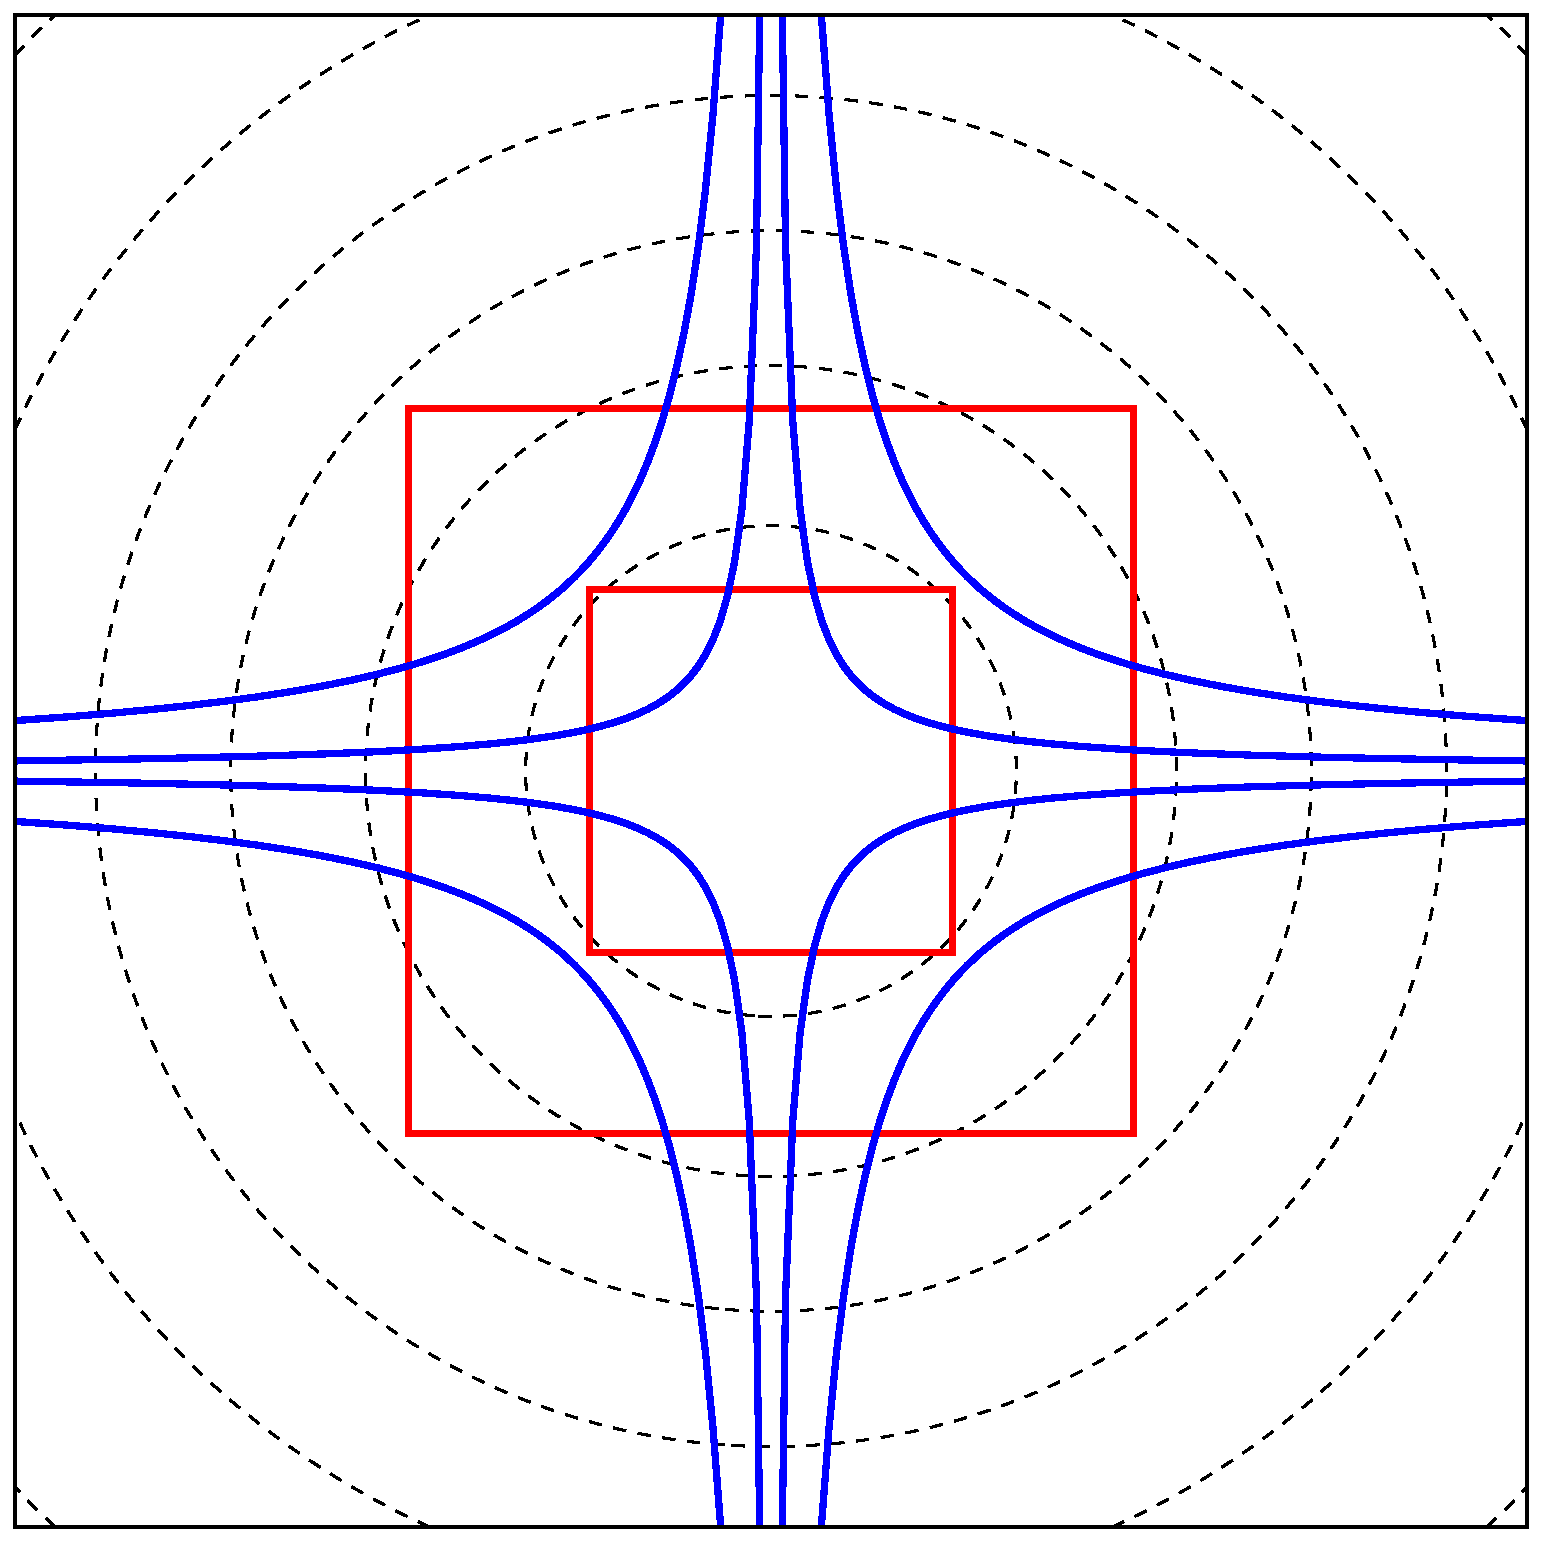
\includegraphics[width=6cm]{figs/hcboltz/hcgauss}
    \caption{Contour plot of the amplitude of the spectrum of a Gaussian, with the
             Fourier modes belonging to hyperbolic crosses and full grids of
             comparable size delineated for comparison. It seems that full
             grids offer much better approximation of Gaussians.}
    \label{fig:hcgauss}
\end{figure}

This indicates that the hyperbolic cross would be a poor choice for approximating
near-equilibrium solutions.  Of course, it could still provide a useful tool for
certain situations with $f$ far removed from equilibrium.  Moreover, the results
in this paper are not confined to the classical hyperbolic cross ($Y=0$) but to
the whole family of sampling sets $\cA_Y$, as well as $\AFF$, which allows
fine-tuning according to the degree of isotropy in the solution.

\subsection{Observables}

For the linear functionals mass density ($\rho$), momentum ($\Bu$) and energy ($E$), which define the
equilibrium solution, we have representations in terms of the coefficients $\hf_\Bk$ from \eqref{eqn:fn}:
\begin{gather*}
    \rho(f) = \frac{1}{(2L)^d}\sum_{\Bk\in\cA} \hat{\rho}_\Bk\hf_\Bk, \quad
    (\rho\Bu)(f) = \frac{1}{(2L)^d}\sum_{\Bk\in\cA} \hat{\Bu}_\Bk\hf_\Bk\\
    (\rho E)(f) = \frac{1}{(2L)^d}\sum_{\Bk\in\cA} \hat{E}_\Bk\hf_\Bk.
\end{gather*}
The quantities $\hat{\rho}_\Bk$, $\hat{\Bu}_\Bk$ and $\hat{E}_\Bk$ are given as
(re-scaled) Fourier coefficients of the functions $1$, $\Bv$ and $|\Bv|^2$:
\[
    \frac{1}{(2L)^d}
    \begin{pmatrix} 
        \hat{\rho}_\Bk \\ \hat{\Bu}_\Bk \\ \hat{E}_\Bk 
    \end{pmatrix} 
    = \int_{\cD_L} 
    \begin{pmatrix} 
        1 \\ \Bv \\ |\Bv|^2 
    \end{pmatrix} 
    e^{i\Bk\cdot \Bv} \dd \Bv
\]

Clearly, for mass density, we have $\hat{\rho}_\Bk = (2L)^d\delta_{\Bk,\Bzero}$.

For $\Bu$ and $E$, we find that $\hat{\Bu}_\Bk = \hat{E}_\Bk = 0$ whenever
$\Bk$ is off the axes, i.e. there is more than one nonzero element of $\Bk$.
Thus, let $\Bk = \frac{\pi}{L}\tilde{k}_j\Be_j$, where $\Be_j$ is the $j$'th
Cartesian basis vector, and $\tilde{k}_j$ some integer. 

Then we obtain
\begin{align*}
    (\hat{\Bu}_\Bk)_l &= 
    \begin{cases} 
        -i\frac{(-1)^{\tilde{k}_j}}{k_j}, & l=j \quad\text{and}\quad 
                \Bk\neq\Bzero \\ 
        0, & l\neq j \quad\text{or}\quad \Bk = \Bzero. 
    \end{cases} \\
    \hat{E}_\Bk &= 
    \begin{cases} 
        2\frac{(-1)^{\tilde{k}_j}}{k_j^2}, & \Bk\neq\Bzero, \\
        \frac{d}{3}L^2, & \Bk = \Bzero.
    \end{cases}
\end{align*}

Thus we see that even if $\cA$ is relatively large, say a box of $N^d$ degrees
of freedom, the accurate evaluation of these functionals require only a subset
of $\cA$ containing the axes, which are of size $\cO(dN)$.

It's also worth noting that $\AFF(N) \supseteq \cA_Y(N)$, yet for any functional
$\ell$ that depends only on Fourier coefficients on the axes (such as $\rho$,
$\Bu$ and $E$), we have
\[
    \ell\left(P_{\cA_Y(N)}f\right) = \ell\left(P_{\AFF(N)}f\right).
\]
The full grid offers no advantage over $\cA_Y$ in terms of such functionals, although off-axis modes will of
course impact the on-axis modes during evolution.

\subsection{Cost of evaluating $P_\cA Q^R(f_\cA,f_\cA)$}

The evaluation of $Q(f_\cA,f_\cA)$ requires the formation of the sum \eqref{eqn:boltzmann-d}. There are no
fast algorithms to compute this, unless some kind of separability of $\hbeta$ is available, as in
\cite{Mouhot06}, which seems to be the case only for certain specific kernels $B$. In these cases the sum has
a convolution structure and we can evaluate the collision operator by using an FFT method requiring log-linear
time ($\cO(dN\log(N))$, where $N$ is the number of degrees of freedom in one dimension).

Without this convolution structure, a straightforward naive implementation has cost proportional to the
cardinality of the combination set
\[
    c(\cA) = \left\{ (\Bl,\Bm)\in\cA^2 \;:\; \Bl+\Bm\in\cA \right\}.
\]
The worst possible case for any $\cA$ is $\sharp c(\cA(N)) \in \cO([\sharp \cA(N)]^2)$, and for the the full grid
this bound is sharp. However, the hyperbolic cross can do better. For $Y=0$, we have experimentally that
\[
    \sharp c(\cA_0(N)) \in \cO(\sharp\cA_0(N)^{\nicefrac{15}{8}}),
\]
see Figure \ref{fig:complexity}.

\begin{figure}
    \centering
    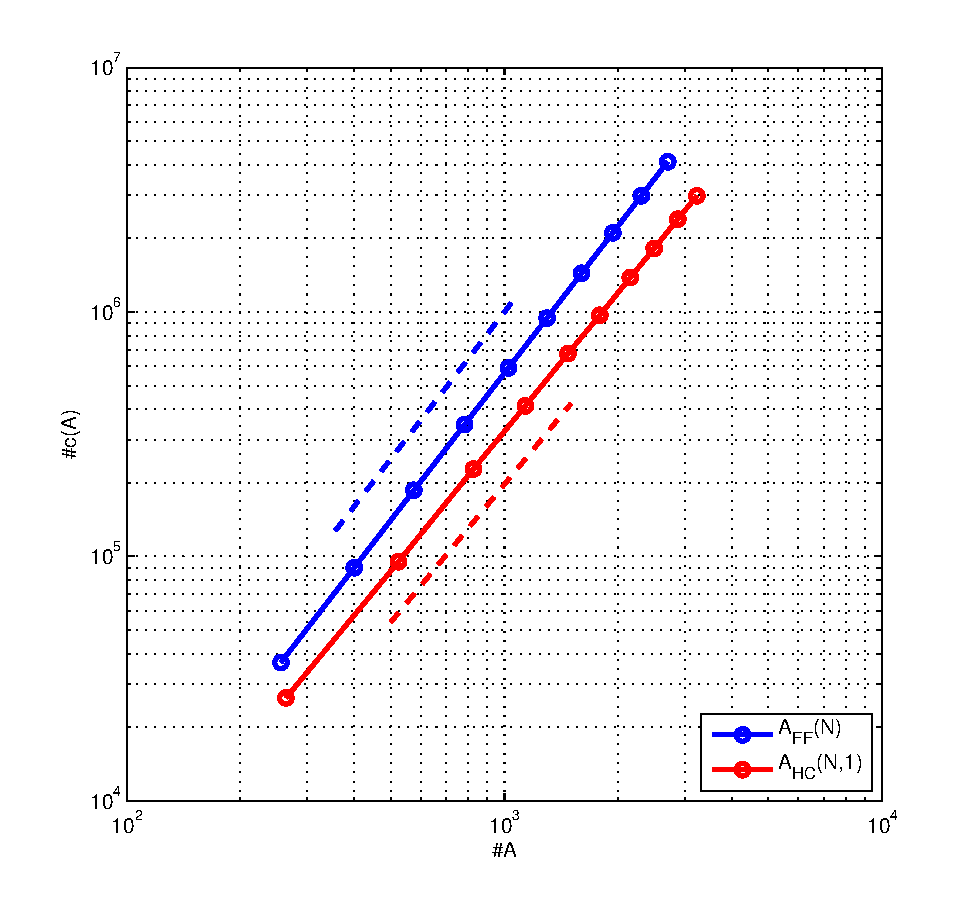
\includegraphics[width=12cm]{figs/hcboltz/complexity}
    \caption{Logarithmic plot of $\sharp c(\cA)$ versus $\sharp\cA$ for $\AFF(N)$
        (blue) and $\cA_0(N)$ (red), showing a minor improvement in complexity
        for the hyperbolic cross. The dashed lines represent $y=c_1x^2$ and
        $y=c_2x^{\nicefrac{15}{8}}$.}
    \label{fig:complexity}
\end{figure}

\section{Approximation Error} \label{sec:appr}

When necessary, we will assume hyperbolic cross approximations to give specific
rates, however the theory is equally valid for full spaces.

We are primarily concerned with the dependence of the errors on the
discretization parameters $N$ and $L$. In line with Section~\ref{sec:trunc} we
will assume the ratio
$$
    \frac{R}{L} = \kappa
$$
for some fixed $\kappa>0$.

Throughout the section, we will take Assumption~\ref{ass:B} for granted. We
also make use of the notation
$$
    \ml = \max(0,\lambda) \quad\text{for $\lambda$ from \eqref{eq:CrossRep},}
$$
as well as the simplification $Q(f) \defeq Q(f,f)$ for the symmetrical application of $Q$.

Constants that do not depend on the truncation parameters $L$, $R$, the
discretization parameters $Y$, $N$, or $f$ are suppressed. Thus, a
statement such as $A\lesssim B$ means that there exists some quantity $C$ that
does not depend on $L$, $R$, $Y$, $N$ or $f$, such that $A \leq CB$.

\subsection{Basic estimates}

Our first result is a boundedness result for $Q^R$ in $L^2$ for periodic
functions. 
\begin{theorem}\label{thm:L2bound}
  Under Assumption \ref{ass:B} we have for functions $f,g$, which are $2L$-periodic
  with fundamental domain $\cD_L=[-L,L]^d$, the estimate
    \[
        \|Q^R(f,g)\|_\LtDl\lesssim L^{2\ml+\nicefrac{d}{2}}
                \|f\|_\LtDl\|g\|_\LtDl, \qquad \forall f,g\in L^2(\cD_L).
    \]
    Moreover, the function $Q^R(f,g)$ is $2$-periodic. 
\end{theorem}
The proof of this theorem treats the gain- and loss term separately.  In order
to handle the gain term we need the following result from \cite[Theorems 1,
2]{Alonso10}.  
\begin{theorem}\label{thm:L2boundGain}
    If $\lambda \geq 0$, with constants also depending on $\lambda$,
    \[
        \|Q^{R,+}(f,g)\|_\LtDl \lesssim
                \|f\|_{L^2_\lambda(\cD_{\tilde{\kappa}L})}
                \|g\|_{L^1_\lambda(\cD_{\tilde{\kappa}L})},\qquad \forall
                f,g\in L^2_\lambda(\cD_{\tilde{\kappa}L}),
    \]
    where $\tilde{\kappa}=\sqrt{2}+2\kappa$, and we define for $\nu>0$, $p\geq 1$, and a domain $D\subseteq
    \mathbb{R}^d$
    \[
        \|f\|_{L^p_\nu(D)}^p:=\int_{D} |f(\Bv)|^p(1 + |\Bv|^{p\nu})\dd\Bv. 
    \]
    For $-d <\lambda <0$ and 
    \[
        \frac{1}{p} + \frac{1}{q} = 1 + \frac{\lambda}{d}+\frac{1}{r} 
    \]
    we have
    \[
        \|Q^{R,+}(f,g)\|_{L^r(\cD_L)} \lesssim
        \|f\|_{L^p(\cD_{\tilde{\kappa}L})}\|g\|_{L^q(\cD_{\tilde{\kappa}L})}\qquad \forall f\in
        L^p(\cD_{\tilde{\kappa}L}), g\in L^q(\cD_{\tilde{\kappa}L})
    \]
\end{theorem}
\begin{proof}
    This result has been shown in \cite[Theorems 1, 2]{Alonso10} for the
    non-truncated gain operator $Q^+$ and with the norms for the terms
    $Q^{R,+}(f,g), f, g$ taken over all of $\mathbb{R}^d$ instead of bounded subsets.

    As to the effect of the truncation we remark that exactly the same
    arguments as in \cite{Alonso10} apply to the truncated case by replacing
    \[
        B(|\Bg|,\cos\theta)\leftrightarrow 
                B(|\Bg|,\cos\theta)\chi_{\mathcal{B}_{2R}},
    \]
    with $\chi_{\mathcal{B}_{2R}}$ denoting the indicator function of
    $\mathcal{B}_{2R}$.

    To justify the fact that in our estimates the norms on the right-hand sides
    are just taken over $[-\tilde{\kappa}L,\tilde{\kappa}L]^d$ we remark that by the definition of
    $Q^{R,+}$, the values of $Q^{R,+}(f,g)(\Bv)$ for $\Bv\in [-L,L]^d$ depend only
    on $f$ and $g$ restricted to $[-\tilde{\kappa}L,\tilde{\kappa}L]^d$.
\end{proof}
\begin{proof}[Proof of Theorem \ref{thm:L2bound}]
    We first show the desired statement for the loss term
    \begin{align*}
        Q^{R,-}(f,g)(\Bv) 
        &= \int_{\mathcal{B}_{2R}}\int_{\bbS^{d-1}}B(|\Bu|,\cos\theta)
            g(\Bv-\Bu)\dd\Bsigma\dd\Bu\cdot f(\Bv) \\
        &= \left(A_\lambda\ast g\right)(\Bv)\cdot f(\Bv),
    \end{align*}
    where
    \[
        A_\lambda(\Bu) := \int_{\bbS^{d-1}} B(|\Bu|,\cos\theta) \dd\Bsigma = |\Bu|^\lambda A(\Bu),
    \]
    where $A$ is called the total cross-section.  Since the integral runs over a bounded domain and, by Grad's
    cutoff assumption \eqref{eq:Grad}, $A_\lambda$ is uniformly bounded if $\lambda>0$, and we can assume
    \[
        \|A_\lambda\|_{L^\infty(\cD_L)} \lesssim L^{\ml},
    \]
    which entails 
    \begin{align}
        \|Q^{R,-}(f,g)\|_{L^2(\cD_L)} & \le \|f\|_{L^2(\cD_L)}
                \|A_\lambda\ast g\|_{L^\infty(\cD_L)} \\
        \label{eq:lossbound} & \le \|f\|_{L^2(\cD_L)}
                \|A_\lambda\|_{L^\infty(\cD_L)}\|g\|_{L^1(\cD_{\tilde{\kappa}L})}.
    \end{align}
    The last inequality holds since only the values of $g$ restricted to
    $[-\tilde{\kappa}L,\tilde{\kappa}L]^d$ are used for the evaluation of $A_\lambda\ast g(\Bv)$, $\Bv\in
    [-L,L]^d$.

    If $\lambda<0$, $A_\lambda$ is still integrable by the assumption $\lambda\ge
    -\nicefrac{d}{2}$. Thus, $A_\lambda$ has bounded Fourier transform, and the
    convolution operator is bounded in $L^2$.  We can further estimate
    \[
        \|g\|_{L^1(\cD_{\tilde{\kappa}L})}\lesssim 
        L^{\nicefrac{d}{2}}\|g\|_{L^2(\cD_{\tilde{\kappa}L})}.
    \]
    Now we observe that, due to periodicity of $g$, the previous quantity can be bounded by a constant
    times
    \[
        L^{\nicefrac{d}{2}}\|g\|_{L^2(\cD_L)}
    \]
    Plugging this estimate into (\ref{eq:lossbound}) yields the desired
    estimate for the loss term.

    For the gain term we first focus on the case $\lambda \geq 0$, in which
    case we appeal to the first part of Theorem \ref{thm:L2boundGain}, which
    states that
    \begin{equation}\label{eq:l2rest0}
        \|Q^{R,+}(f,g)\|_{\LtDl} \lesssim
                \|f\|_{L^2_\lambda(\cD_{\tilde{\kappa}L})}\|g\|_{L^1_\lambda(\cD_{\tilde{\kappa}L})}.
    \end{equation}
    Since $f$ and $g$ are periodic, we have
    \begin{equation}\label{eq:l2rest1}
        \|Q^{R,+}(f,g)\|_{\LtDl} \lesssim
                \|f\|_{L^2_\lambda(\cD_L)}\|g\|_{L^1_\lambda(\cD_L)}.
    \end{equation}
    Since 
    \[
        \|f\|_{L^p_\lambda(\cD_L)}\lesssim L^\lambda\|f\|_{L^p(\cD_L)}
    \]
    for all $p\geq 1$ and 
    \[
        \|g\|_{L^1(\cD_L)}\lesssim L^{\nicefrac{d}{2}} \|g\|_{L^2(\cD_L)},
    \]
    we arrive at
    \[
        \|Q^{R,+}(f,g)\|_{L^2(\cD_L)} \lesssim L^{\nicefrac{d}{2}+2\lambda}
                \|f\|_{L^2(\cD_L)}\|g\|_{L^2(\cD_L)}
    \]
    whenever $\lambda \geq 0$.
    
    Now we turn to the case $-\nicefrac{d}{2} \le \lambda <0$.  By our assumptions on $d$
    and $\lambda$, we can find $p,q \le 2$ such that with $r=2$ we have
    \[
        \frac{1}{p} + \frac{1}{q} = 1 + \frac{\lambda}{d}+\frac{1}{r}
    \]
    By the second part of Theorem \ref{thm:L2boundGain} and arguing as above,
    we get
    \[
        \|Q^{R,+}(f,g)\|_{L^2(\cD_L)} \lesssim L^{\nicefrac{d}{2}}
                \|f\|_{L^2(\cD_L)}\|g\|_{L^2(\cD_L)},
    \]
    using the estimate
    \[
        \|f\|_{L^p(\cD_{\tilde{\kappa}L})} \lesssim L^{\nicefrac{d}{p}-\nicefrac{d}{2}} 
                \|f\|_{L^2(\cD_L)}
    \]
    and choosing
    \[
        \frac{2}{p}=\frac{2}{q}=\frac{3}{2}+\frac{\lambda}{d} \le \frac{3}{2}.
    \]
    This yields the desired estimate.
    
    To see that also $Q^R(f,g)$ is $L$-periodic, we simply write both $f$ and
    $g$ as a Fourier series which directly yields the Fourier series
    representation of Section~\ref{sec:FourierDiscretization} for $Q^R(f,g)$.
    This proves the theorem.
\end{proof}
The second result we will require is a product rule for derivatives
of the collision operator which can be found in \cite{Villani98}.
\begin{proposition}\label{prop:prodrule}
    We have 
    \[
        \partial_j Q^R(f,g) = Q^R(\partial_j f, g) + Q^R(f,\partial_j g),
    \]
    where $\partial_j$ denotes the derivative in the $j$-th coordinate
    direction.
\end{proposition}
\begin{proof}
    This result has been proven in \cite{Villani98}, but we give a simpler
    proof which applies to the case when $f$ and $g$ are $2L$-periodic, which
    is of interest to us. In this case we can write
    \begin{align*}
        \mathcal{F}(\partial_j Q^R(f,g))(\Bk)
            &= \sum_{\Bl+\Bm = \Bk}\hat\beta(\Bl,\Bm)\ii k_j\hat f_\Bl \hat g_\Bm
            \\
            &= \sum_{\Bl+\Bm = \Bk}\hat\beta(\Bl,\Bm)\ii l_j\hat f_\Bl \hat g_\Bm
            + \sum_{\Bl+\Bm = \Bk}\hat\beta(\Bl,\Bm)\hat f_\Bl \ii m_j\hat g_\Bm.
    \end{align*}
    The latter sum is equal to
    \[
        \mathcal{F}(Q^R(\partial_jf,g))(\Bk)+
                \mathcal{F}(Q^R(f,\partial_j g))(\Bk)
    \]
    which proves the statement.
\end{proof}

\subsection{Consistency}
In the following we will develop estimates for the consistency error
\[
    \|Q^R(f,f) - \PA Q^R(\PA f,\PA f)\|_{H^s(\cD_L)},
\]
where $\PA$ denotes the projection operators onto the Fourier modes contained
in $\cA$.

If the support of $f$ lies in a ball $\B_R$, by Proposition \ref{prop:equiv} such a bound yields error bounds
for the $H^s$-norm of the error between the application of the discretized collision operator $\PA Q^R(\PA
f,\PA f)$ and the application of the truncated operator $Q^R(f,f)$ in terms of $f$.  These results generalize
the results of \cite{Pareschi00} to more general sets of Fourier modes. 

We will examine this consistency error for a family of different Fourier
discretizations. Only for simplicity we will assume $L = 1$ and, therefore, all
function spaces to follow are defined on $[-1,1]^d$. The case of general $L$ is
hardly more difficult, but it would require heavier notation.

The corresponding smoothness spaces are the following \emph{mixed Sobolev spaces}
as defined in \cite{Knapek00}.
\begin{definition}
    We define the smoothness spaces
    \begin{equation}
        {H}_{\mathrm{mix}}^{t,l}(\cD_L):=
        \left\{
            f\in L^2(\cD_L) \;:\; \sum_{\substack{|\Balpha|_\infty \le t\\
            |\Bbeta|_1 \le l}}\left\|\partial^\Balpha 
                    \partial^\Bbeta f\right\|_{L^2(\cD_L)} <\infty
        \right\}.
    \end{equation}
\end{definition}
\begin{remark}
    For $t=0$ we get the usual Sobolev spaces, for $l=0$ we get the Sobolev
    spaces with dominating mixed smoothness.
\end{remark}
In \cite{Knapek00} the following approximation result is shown.
\begin{theorem}\label{thm:Knapek}
    We have
    \[
        \|f - \mathcal{P}_{\mathcal{A}_Y(N)}f\|_{H^s(\cD_L)} \lesssim 
            (1+N)^{\rho} \|f\|_{{H}_{\mathrm{mix}}^{t,l}(\cD_L)} 
    \]
    Where
    \begin{equation} \label{eq:hcrate}
        \rho = \rho(s,l,t,Y,d) = \begin{cases}
            s-l-t+(Yt-s+l)\frac{d-1}{d-Y},& Y\geq\frac{s-l}{t}, \\
            s-l-t,& Y\leq\frac{s-l}{t}. \end{cases}
    \end{equation}
\end{theorem}
In the remainder of the present section we establish the important fact that
the previous optimal approximation order can be retained for the application of
the truncated collision operator.

A crucial tool will be the following boundedness result for the
collision operator.
\begin{theorem}\label{thm:CollSmooth}
    Under the assumptions of Theorem \ref{thm:L2bound} we have that
    \begin{equation}
        \left\|Q^R(f,g)\right\|_{{H}_{\mathrm{mix}}^{t,l}(\cD_L)}
            \lesssim 
                L^{2\ml+\nicefrac{d}{2}}
                \|f\|_{{H}_{\mathrm{mix}}^{t,l}(\cD_L)}
                \|g\|_{{H}_{\mathrm{mix}}^{t,l}(\cD_L)}.
    \end{equation}
\end{theorem}
\begin{proof}
    Note that by Proposition \ref{prop:prodrule}, every derivative
    $\partial^\Balpha Q^R(f,g)$ can be expressed as a linear combination of
    terms 
    \[
        Q^R(\partial^{\Balpha_1}f,\partial^{\Balpha_2}g), \quad \Balpha_1 +
                \Balpha_2 = \Balpha.
    \]
    It follows that we can estimate
    \[
        \|\partial^\Balpha Q^R(f,g)\|_{L^2(\cD_L)} \lesssim 
                \sum_{\Balpha_1 + \Balpha_2 = \Balpha}
                \|Q^R(\partial^{\Balpha_1}f,\partial^{\Balpha_2}g)\|_{L^2(\cD_L)}.
    \]
    Now we can apply Theorem \ref{thm:L2bound} to the summands in the above
    expression and arrive at the desired result.
\end{proof}
The following theorem is our main result concerning the approximation error in
the Fourier discretization of the collision operator.
\begin{theorem}\label{thm:mainapprox}
    We have the estimate 
    \begin{multline*}
        \left\|Q^R(f) - P_{\cA_Y(N)} Q^R(P_{\cA_Y(N)}f)\right\|_{H^s(\cD_L)} \lesssim
            L^{2\ml+\nicefrac{d}{2}}
            (1+N)^\rho \|f\|_{{H}_{\mathrm{mix}}^{t,l} (\cD_L)}^2 ,
    \end{multline*}
    where $\rho=\rho(s,l,t,Y,d)$ is given by \eqref{eq:hcrate}.
\end{theorem}
\begin{proof}
    We write
    \begin{multline*}
        \left\|Q^R(f) - P_{\cA_Y(N)} Q^R(P_{\cA_Y(N)}f)\right\|_{H^s(\cD_L)} \\
        \le \left\|Q^R(f) - P_{\cA_Y(N)} Q^R(f)\right\|_{H^s(\cD_L)} \\
                + \left\|P_{\cA_Y(N)}Q^R(f) - P_{\cA_Y(N)}
                Q^R(P_{\cA_Y(N)}f)\right\|_{H^s(\cD_L)}.
    \end{multline*}
    Since the operator $P_{\cA_Y(N)}$ is a Fourier projection, this can be further
    bounded from above by
    \[
        \left\|Q^R(f) - P_{\cA_Y(N)} Q^R(f)\right\|_{H^s(\cD_L)} + 
        \left\|Q^R(f) - Q^R(P_{\cA_Y(N)}f)\right\|_{H^s(\cD_L)}.
    \]
    To handle the first term we first invoke Theorem \ref{thm:Knapek}
    to obtain  
    $$
        \left\|Q^R(f) - P_{\cA_Y(N)} Q^R(f)\right\|_{H^s(\cD_L)} \lesssim 
            (1+N)^\rho \|Q^R(f)\|_{{H}_{\mathrm{mix}}^{t,l}(\cD_L)}
    $$
    Now, all we need to do is to estimate the quantity 
    $\|Q^R(f)\|_{{H}_{\mathrm{mix}}^{t,l}(\cD_L)}$ in terms of the
    mixed Sobolev norm of $f$, which has been done in Theorem
    \ref{thm:CollSmooth}.

    This takes care of the first term.  In order to estimate the second term,
    given by
    \[
        \left\|Q^R(f) - Q^R(P_{\cA_Y(N)}f)\right\|_{H^s(\cD_L)},
    \]
    we invoke the bilinearity of $Q^R$ which allows us to rewrite this
    expression as 
    \[
        \left\|Q^R\left(f - P_{\cA_Y(N)}f,f\right) + Q^R\left(
                P_{\cA_Y(N)}f,f-P_{\cA_Y(N)}f\right) \right\|_{H^s(\cD_L)}.
    \]
    Now we can invoke the bound of Theorem \ref{thm:CollSmooth} with $t=0$ and
    $l=s$ to bound this quantity by 
    \[
        L^{2\ml+\nicefrac{d}{2}}
        \left\|f - P_{\cA_Y(N)}f\right\|_{H^s(\cD_L)} 
                \left(\left\|f\right\|_{H^s(\cD_L)}+
                \left\|P_{\cA_Y(N)}f\right\|_{H^s(\cD_L)} \right).
    \]
    The first factor in this product can be estimated using Theorem
    \ref{thm:Knapek}, the second one is bounded by
    \[
        2\left\|f\right\|_{H^s(\cD_L)}
    \]
    due to the properties of Fourier projections. Summing up these estimates and bounding 
    $\|\cdot\|_{H^s(\cD_L)}$ by $\|\cdot\|_{{H}_\mathrm{mix}^{t,l}(\cD_L)}$
    we arrive at the desired result.
\end{proof}
\begin{remark}
    The previous result paves the way for adaptively enlarging or shrinking
    the set of active Fourier modes in each timestep.  To this end, we envision
    to solve the homogeneous Boltzmann equation over three Fourier grids,
    corresponding to different values of $T$ and decide to switch to a
    larger or smaller grid based on the relative errors between these three
    different solutions.  We consider this approach to be especially promising
    in cases where the solution is well-approximable by a sparse (HC-type) grid
    initially. As the solution approaches the Maxwellian distribution, the
    approximation grid can be modified to yield a full Fourier grid more
    suitable for the approximation of radially symmetric functions.  We leave
    the further exploration of this idea to future work.
\end{remark}

\subsection{Error for the projected equation} \label{sec:evolerr}

The aim of the remainder of Section~\ref{sec:appr} will be to establish
estimates for the error $\|f_\cA - f\|$, where $f$ is the solution to the actual
Boltzmann equation
\[
    \frac{\partial}{\partial t}{f} = Q(f,f), \qquad f(0) = f_0,
\]
and $f_\cA$ is the solution to the truncated and projected equation
\[
    \frac{\partial}{\partial t}{f}_\cA = P_\cA Q^R(f_\cA, f_\cA), \qquad f_\cA(0) = P_\cA f_0.
\]
We will also require the intermediate solution of the truncated, but not
projected, equation
\[
    \frac{\partial}{\partial t}{f}_R = Q^R(f_R, f_R), \qquad f(0) = f_0.
\]
Due to the periodicity of $f_\cA$, the error will necessarily have to be
estimated on a bounded domain.

In Section~\ref{sec:extfilb} we will estimate the error $\|f_\cA-f_R\|$ by relying
on work by Filbet and Mouhot \cite{Filbet11}. In Section~\ref{sec:err-trunc} we
will estimate the error $\|f_R-f\|$ due to truncation.

Throughout, we will make Assumption \ref{ass:B} and in Section~\ref{sec:err-trunc}
we make the assumption that Conjecture~\ref{ass:decay} holds.

To ease notation we will also write $\cA=\cA_Y(N)$ when necessary to obtain specific rates, although the
theory remains true for general $\cA$.

\subsubsection{Error due to discretization} \label{sec:extfilb}

First, we will aim to generalize the non-global results of \cite{Filbet11}, by
which me mean everything up to, and including, \cite[Proposition
4.6]{Filbet11}\footnote{The remainder of \cite{Filbet11} involves global estimates under an assumption of
  $\kappa\geq\sqrt{2}$. This assumption appears non-physical, however, and causes heavy aliasing, see 
  Section~\ref{sec:aliasing}.}. The program involves studying a perturbation from the {\em
  truncated} equation, of the form
\begin{equation} \label{eqn:pert}
    \frac{\partial}{\partial t}{f}_\cA = Q^R(f_\cA) + r_\cA
\end{equation}
where the residual term $r_\cA$ has the form
\[
    r_\cA = (P_\cA-\idty)Q^R(f_\cA).
\]

First, let us recall
\begin{lemma}\label{lem:bound}
  Assume $g$ and $h$ are $2L$-periodic functions on $\bbR^d$, and that $B$ is
  separable with a power law dependence on the relative velocity with
  exponent $\lambda \geq -\nicefrac{d}{2}$, satisfying Grad's cutoff assumption
  \eqref{eq:Grad}. Then, for all $p\in [1,\infty]$
    $$ 
        \|Q^R(g,h)\|_{L^p(\cD_L)},\ \|Q^R(h,g)\|_{L^p(\cD_L)} \lesssim 
            L^{2\ml} \|g\|_{L^1(\cD_L)}
            \|h\|_{L^p(\cD_L)}. 
    $$
\end{lemma}
\begin{proof}
This is a straightforward generalization of the proofs of Theorems
\ref{thm:L2bound} and \ref{thm:L2boundGain}. It is also the content of 
\cite[Lemma 4.1]{Filbet11}.
\end{proof}

Furthermore we have the product rule from Proposition~\ref{prop:prodrule}
\begin{equation}\label{eq:prodrule}
    \partial^\Balpha Q^R(g,h)=Q^R(\partial^\Balpha g,h)+Q^R(g,\partial^\Balpha h),
\end{equation}
for all $\Balpha \in \mathbb{N}^d$, $|\Balpha| = 1$. It is straightforward to
obtain a similar Leibniz-type product formula for general $\Balpha \in
\mathbb{N}^d$.
\begin{definition} \label{def:spaces}
    Let $\Balpha\in \mathbb{N}^d$. Then define the smoothness 
    spaces $H^\Balpha(\cD_L)$, $H^{<\Balpha}(\cD_L)$ with norms
    $$
        \|g\|_{H^\Balpha(\cD_L)}:= \sum_{\Bzero \leq \Bbeta \le \Balpha}\|\partial^\Bbeta g
        \|_{L^2(\cD_L)},\quad
        \|g\|_{H^{<\Balpha}(\cD_L)}:= \sum_{\Bzero \leq \Bbeta < \Balpha}\|\partial^\Bbeta g
        \|_{L^2(\cD_L)},
    $$
    where the vector inequalities $\Bbeta \leq \Balpha$ and $\Bbeta < \Balpha$ are to be understood
    element-wise.
\end{definition}
\begin{remark}
    Note that we have
    %
    $$
        \|g\|_{{H}_{\mathrm{mix}}^{t,l}(\cD_L)}
        \lesssim \sum_{\substack{|\Balpha_1|_\infty=t\\ |\Balpha_2|_1=l}}
        \|g\|_{H^{\Balpha_1+\Balpha_2}(\cD_L)},
    $$
    %
    so any smoothness result which applies to all norms 
    $\|g\|_{H^\Balpha(\cD_L)}$ also applies to the mixed smoothness
    Sobolev norms.
\end{remark}
Note that for any $\cA$ and $\Balpha\in\bbN^d$, it is obvious that
\begin{equation}\label{eq:contr}
    \|\partial^\Balpha P_\cA f\|_{L^2(\cD_L)} \le \|\partial^\Balpha f\|_{L^2(\cD_L)}.
\end{equation}
\begin{lemma}\label{lem:boundsmooth}
    Let $\Balpha \in \mathbb{N}^d$. Then we have
    $$
        \|Q^R(f)\|_{H^\Balpha(\cD_L)},\ \|P_\cA Q^R(f)\|_{H^\Balpha(\cD_L)}
        \lesssim L^{2\ml+\nicefrac{d}{2}} 
        \|f\|_{H^{<\Balpha}(\cD_L)}
        \|f\|_{H^\Balpha(\cD_L)}.
    $$
\end{lemma}
\begin{proof}
    By (\ref{eq:contr}) it suffices to show the estimate for $Q^R(f,f)$. 
    Hence we get
    \begin{eqnarray*}
        \|\partial^\Balpha Q^R(f,f)\|_{L^2(\cD_L)}
        & \lesssim &
        L^{2\ml}\sum_{\Bzero \le \Bbeta \le \Balpha}
        \|\partial^\Bbeta f \|_{L^1(\cD_L)} 
        \|\partial^{\Balpha - \Bbeta}f\|_{L^2(\cD_L)} \\
        & \lesssim &
        L^{2\ml+\nicefrac{d}{2}}\sum_{\Bzero \le \Bbeta \le \Balpha}
        \|\partial^\Bbeta f \|_{L^2(\cD_L)}
        \|\partial^{\Balpha - \Bbeta}f\|_{L^2(\cD_L)}
        \\
        &\lesssim &
        L^{2\ml+\nicefrac{d}{2}} \sum_{\Bzero \le \Bbeta <\Balpha}
        \|\partial^\Bbeta f \|_{L^2(\cD_L)} 
        \|f\|_{H^\Balpha(\cD_L)}.
    \end{eqnarray*}
    We have used the product rule (\ref{eq:prodrule}), the bound of Lemma
    \ref{lem:bound} and the fact that the $1$-norm can be bounded by the
    $2$-norm on compact sets.

    The implicit constant depends on the implicit constant from Lemma
    \ref{lem:bound} and a combinatorial expression depending on $\Balpha$.
\end{proof}
These results allow us to state the following analogue of \cite[Lemma
4.2]{Filbet11}:
\begin{lemma}\label{lem:prop}
    Consider the evolution problem \eqref{eqn:pert} and
    assume that we have a uniform $L^1$-bound 
    \begin{equation}
        \sup_{t\in [0,T_\mathrm{max}]}\|f_\cA(t,\cdot)\|_{L^1(\cD_L)}\le M.
    \end{equation}
    Then for any $\Balpha \in \bbN^d$, and $f_0\in H^\Balpha(\cD_L)$, there exists
    a quantity $C_\Balpha$, depending only on $M,L,T$ and
    $\|f_0\|_{H^{\Balpha}(\cD_L)}$ such that
    \begin{equation}\label{eq:smoothprop}
        \sup_{t\in [0,T_\mathrm{max}]}\|f_\cA(t,\cdot)\|_{H^\Balpha(\cD_L)}
        \le C_\Balpha(L).
    \end{equation}
\end{lemma}
\begin{proof}
    For $0\le k \le |\Balpha|_1$ we denote the sets
    $$
        A_\Balpha^k:=\left\{\Bbeta \in \mathbb{N}^d \;:\;
        \Bbeta \le \Balpha \mbox{  and  }|\Bbeta|_1 = k\right\}.
    $$
    We will show inductively that for all such $k\in \mathbb{N}$, there exists a
    constant $C_k(L)<\infty$ such that
    \begin{equation}\label{eq:ind}
        \sup_{t\in [0,T]}\sup_{\Bbeta \in A_\Balpha^k}
        \|f_\cA(t,\cdot)\|_{H^\Bbeta(\cD_L)}\le C_k(L).
    \end{equation}
    Clearly, (\ref{eq:ind}) with $k=|\Balpha|_1$ is simply the desired
    statement (\ref{eq:smoothprop}).
    
    We start by showing (\ref{eq:ind}) for $k= 0$ which amounts to deriving an
    $L^2$-bound for $f_{\cA}$. To this end consider the ODE
    $$
        \frac12\frac{\fdd}{\fdd t}\|f_\cA\|_{L^2(\cD_L)}^2 \le 
        \|Q^R(f_\cA)+r_\cA\|_{L^2(\cD_L)} \|f_\cA\|_{L^2(\cD_L)}
    $$
    From Lemma \ref{lem:bound} with $p=2$ we deduce that
    $$
        \frac12\frac{\fdd}{\fdd t}\|f_\cA\|_{L^2(\cD_L)}^2 \lesssim
        L^{2\ml} \|f_\cA\|_{L^1(\cD_L)} \|f_\cA\|_{L^2(\cD_L)}^2 \le 
        L^{2\ml} M\|f_\cA\|_{L^2(\cD_L)}^2.
    $$
    Grönwall's lemma yields (\ref{eq:ind}) for $k=0$.
    
    Now the induction step. Assume we have (\ref{eq:ind}) for $k-1$.  Then we
    have for any $\Bbeta \in A_\Balpha^k$ that
    $$
        \frac12\frac{\fdd}{\fdd t}\|f_\cA\|_{H^\Bbeta(\cD_L)}^2 \le 
        \|Q^R(f)+r_\cA\|_{H^\Bbeta(\cD_L)} \|f_\cA\|_{H^\Bbeta(\cD_L)}.
    $$
    Now, Lemma \ref{lem:boundsmooth} yields that
    \begin{align*}
        \frac12\frac{\fdd}{\fdd t}\|f_\cA\|_{H^\Bbeta(\cD_L)}^2 & \lesssim
        L^{2\ml+\nicefrac{d}{2}} \|f_\cA\|_{H^{<\Bbeta}(\cD_L)}
        \|f_\cA\|_{H^\Bbeta(\cD_L)}\|f_\cA\|_{H^\Bbeta(\cD_L)} \\ 
        & \le L^{2\ml+\nicefrac{d}{2}}C_{k-1}(L)\|f_\cA\|_{H^\Bbeta(\cD_L)}^2.
    \end{align*}
    We have used the induction hypothesis in the last inequality.  Using
    Grönwall's lemma again yields the desired claim.
\end{proof}
The following proposition establishes existence, uniqueness and control of
$L^1$- and $H^\Balpha$-norms.
\begin{proposition}\label{lem:existence}
  Consider the evolution problem \eqref{eqn:pert}, make Assumption
  \ref{ass:B} and set $W=\|P_\cA f_0\|_{L^2(\cD_L)}$.

    Then there exists $\overline{\tau} = \overline{\tau}(W,L) > 0$ so that
    \eqref{eqn:pert} admits a unique solution on $[0,\overline{\tau}]$, and on
    this interval $\|f_\cA(t)\|_{L^1(\cD_L)}$ is bounded.
\end{proposition}
\begin{proof}
  We closely follow \cite[Proposition 4.3]{Filbet11}. Using Lemma
  \ref{lem:bound} with $p=2$, we find that for some $K>0$,
  $$
  \frac{\fdd}{\fdd t}\|f_\cA(t)\|_{L^2(\cD_L)} \le
  KL^{2\ml+\nicefrac{d}{2}}\|f_\cA(t)\|_{L^2(\cD_L)}^2,
  $$
  yielding
  $$
  \|f_\cA(t)\|_{L^2(\cD_L)} \leq \frac{\|P_\cA f_0\|_{L^2(\cD_L)}}
  {1-KL^{2\ml+\nicefrac{d}{2}}\|P_\cA f_0\|_{L^2(\cD_L)}t}.
  $$
  Since $\cD_L$ is bounded, this can be used to show that the $L^1$-norm is
  bounded on $[0,\overline{\tau}]$ provided the interval is small enough. The
  bound is explicit from the above inequality.
  
  Then, existence and uniqueness follows from the theorem of Picard-Lindelöf,
  since $Q^R$ is a bounded bilinear operator from $L^2(\cD_L)\times L^2(\cD_L)$ to
  $L^2(\cD_L)$.
\end{proof}

Uniform control of the $L^2$-norm on $[0,T_\mathrm{max}]$ will, by repeatedly
applying Proposition \ref{lem:existence}, yield existence and uniqueness on
this interval. Then, Lemma \ref{lem:prop} will provide smoothness, assuming
smoothness of the initial condition.

Such control of the $L^1$-norm is clear for the classical (non-perturbed)
Boltzmann equation due to preservation of positivity and mass density. In
\cite{Filbet11}, Lemmas 4.4 and 4.5 provide the following positivity result.
\begin{lemma} \label{lem:positivity}
    Consider the evolution perturbed problem \eqref{eqn:pert}, make Assumption \ref{ass:B},
    and also assume that $f_0\in L^\infty(\cD_L)$ is non-negative, and that it
    satisfies
    $$
        \|f_0-P_\cA f_0\|_{L^\infty(\cD_L)} \to 0
    $$
    as $N\to\infty$.

    Set $M=2\|f_0\|_{L^1(\cD_L)}$. Then there exists $\hat{\tau} \in
    (0,\overline{\tau})$ depending only on $M$, $L$ and $B$, and there exists
    $\hat{N}<\infty$ depending only on $\hat{\tau}$ and $f_0$, such that for
    all $N > \hat{N}$, and for any smooth solution $f_\cA$ to \eqref{eqn:pert},
    we have
    $$
        \forall \Bv\in\cD_L, \qquad f_\cA(\hat{\tau},\Bv) > 0.
    $$
    Furthermore, there exists $\eta(N)$, tending to $0$ as $N\to\infty$, such
    that for all $t\in[0,\hat{\tau}]$, the negative part of $f_\cA$ satisfies
    the bound
    $$
        \|f_\cA^{-}(t)\|_{L^\infty(\cD_L)} \leq \eta(N).
    $$
\end{lemma}
\begin{proof}
    This is exactly \cite[Lemma 4.5]{Filbet11}. The proof is identical.
\end{proof}
The following theorem summarizes the argument, and corresponds to 
\cite[Proposition 4.6]{Filbet11}. It shows propagation of smoothness for the
perturbed Boltzmann equation, and provides an estimate for the error $f_R-f_\cA$.

Its proof employs the following nonlinear generalization of Grönwall's lemma.
\begin{lemma}[Theorem 21 in \cite{Dragomir03}] \label{lem:gron}
    Let $u(t)$ be a non-negative function satisfying
    \[
        u(t) \leq c + \int_0^t\left(au(s)+b\sqrt{u(s)}\right)\dd s
    \]
    where $a>0$ and $b,c\geq0$. Then
    \[
        u(t) \leq \left[\sqrt{c}e^{\nicefrac{at}{2}} + 
                \frac{b}{a}\left(e^{\nicefrac{at}{2}}-1\right)\right]^2.
    \]
\end{lemma}

\begin{theorem} \label{thm:discrerror} Consider the evolution problem
  \eqref{eqn:pert} for a fixed time interval $[0,T_\mathrm{max}]$. In addition, make
  Assumption \ref{ass:B}, and assume that $f_0\in L^\infty(\cD_L) \cap
  {H}^{t,l}_\mathrm{mix}(\cD_L)$ is non-negative, and satisfies
  $$
  \|f_0-P_\cA f_0\|_{L^\infty(\cD_L)} \to 0\quad \text{for } N\to\infty.
  $$
  Then there exists $\hat{N} < \infty$ such that for all $N>\hat{N}$,
    \begin{enumerate}
    \renewcommand{\labelenumi}{(\roman{enumi})}
    \item there is a unique solution $f_\cA(\tau,\cdot)\in {H}^{t,l}_\mathrm{mix}(\cD_L)$ on
    $[0,T_\mathrm{max}]$ to the perturbed equation \eqref{eqn:pert} with initial data $P_\cA f_0$, uniformly
    bounded in $L^1$.
    \item There is $\eta(N)\to0$ as $N\to\infty$ such that for all $\tau\in[0,T_\mathrm{max}]$,
    \[
        \|f_\cA^{-}(\tau,\cdot)\|_{L^\infty(\cD_L)} \leq \eta(N).
    \]
    \item The solution satisfies the error bound
    \begin{multline*}
        \|(f_R-f_\cA)(\tau)\|_{H^s(\cD_L)} \lesssim \\ \left(
        \frac{C_{t+l}(L)^2}{C_s(L)} +
        \|f_0\|_{{H}^{t,l}_\mathrm{mix}}\right)
        (1+N)^{\rho} \exp\left[\gamma L^{2\ml+\nicefrac{d}{2}}C_s(L)\tau\right]
    \end{multline*}
    for some $\gamma>0$ that does not depend on $L$, $s$, $t$, $l$ or $N$, and
    where $\rho=\rho(s,l,t,Y,d)$ is given in \eqref{eq:hcrate}.
    \end{enumerate}
\end{theorem}
\begin{proof}
    Set $M=2\|f_0\|_{L^1(\cD_L)}$. By Proposition \ref{lem:existence}, there
    exists a unique smooth solution to the perturbed problem on some interval
    $[0,\overline{\tau}]$. By Lemma \ref{lem:positivity}, there exists
    $\hat{\tau}\leq\overline{\tau}$ and $\hat{N}$, such that for all
    $N>\hat{N}$, $f_\cA(\hat{\tau},\cdot)$ is positive.

      By preservation of mass density
      (see e.g., \cite[Equation (3.4)]{Filbet11}) and positivity, we thus have
    $$
        \|f_\cA(\hat{\tau})\|_{L^1(\cD_L)} = \|f_0\|_{L^1(\cD_L)} =
        \frac{M}{2}.
    $$
    By Lemma \ref{lem:prop}, $f_\cA(\hat{\tau})$ also retains the smoothness,
    and by Lemma \ref{lem:positivity}, it is positive. Thus we can use
    induction to prove the existence for all of $[0,T_\mathrm{max}]$. The
    $L^1$-bound is $M$, following from Proposition \ref{lem:existence}.

    The error bound can be deduced from the observation
    $$
        \frac{\partial}{\partial t}(f_R-f_\cA) = 
        Q^R_{\mathrm{sym}}(f_R-f_\cA,f_R+f_\cA) - r_\cA
    $$
    where $Q^R_{\mathrm{sym}}$ is the symmetrized collision operator. From
    Theorem \ref{thm:CollSmooth} we have
    \begin{align*}
        \|Q^R_{\mathrm{sym}}(f_R-f_\cA,f_R+f_\cA)\|_{H^s(\cD_L)} & \lesssim
        L^{2\ml+\nicefrac{d}{2}}\|f_R+f_\cA\|_{H^s(\cD_L)}\|f_R-f_\cA\|_{H^s(\cD_L)} \\ 
        & \lesssim L^{2\ml+\nicefrac{d}{2}}C_s(L)\|f_R-f_\cA\|_{H^s(\cD_L)}.
    \end{align*}
    The bound for $r_\cA=(\idty-P_{\cA_T(N)})Q^R(f_\cA)$ comes from Theorem
    \ref{thm:mainapprox}:
    \begin{align*}
        \|r_\cA\|_{H^s(\cD_L)} & \lesssim (1+N)^{\rho}
        \left(1+\|f_\cA\|_{{H}^{t,l}_\mathrm{mix}(\cD_L)}^2\right)
        \\ &\leq L^{2\ml+\nicefrac{d}{2}}(1+N)^{\rho}C_{t+l}(L)^2.
    \end{align*}
    Thus,
    \begin{multline*}
        \frac{\partial}{\partial\tau} \|f_R-f_\cA\|^2_{H^s(\cD_L)} \lesssim
        L^{2\ml+\nicefrac{d}{2}} \Big[ C_s(L)\|f_R-f_\cA\|^2_{H^s(\cD_L)} + \\
        (1+N)^{\rho}C_{t+l}(L)^2\|f_R-f_\cA\|_{H^s(\cD_L)} \Big] .
    \end{multline*}
    Integrating this inequality, and applying Lemma \ref{lem:gron}, as well as
    the initial approximation of $f_0$ (using Theorem \ref{thm:Knapek}), we
    arrive at the desired result.
\end{proof}
Note that all mixed smoothness Sobolev spaces can be written as intersections of spaces of the type
$H^{\Balpha}$ from Definition \ref{def:spaces}, which connects the estimates made in the proof of Theorem
\ref{thm:discrerror} to those from Lemmas \ref{lem:boundsmooth} and \ref{lem:prop}.


\subsubsection{Error due to truncation} \label{sec:err-trunc}

We will now turn our attention to the error induced by truncating the collision
operator, namely $e_R(t) = f(t) - f_R(t)$. In the following, we will assume
that $\kappa$ is sufficiently small so that the evaluation of $Q^R(f)$ in the
ball $\B_R$ requires only values within $\cD_L$. This condition is slightly
stricter than that which was given earlier.

Throughout this section we will make assume the truth of Conjecture~\ref{ass:decay} concerning the decay of
$f_R$.

\begin{definition}
    \label{def:gd}
    Given a Sobolev index $s\geq 0$, we say that a function
    $g:\mathbb{R}^{d}\to\mathbb{R}$ has a Gauss-like decay, if there
    exists $C>0$ and $a>0$ such that 
    $$
        |\partial^\Balpha g(\Bv)| \le C\exp\left(-a|\Bv|^2\right)
    $$
    for all $|\Balpha|_1 \leq s$.
\end{definition}

\begin{lemma} \label{lem:lipschitz} Fix $s>0$ and assume that $g,h$ satisfy
  Gauss-like decay in the sense of Definition~\ref{def:gd}.  Then, for
    sufficiently large $L$ ($2L\geq1$)
    \[
    \|Q^R(g,g) - Q^R(h,h)\|_{H^s(\B_R)} \lesssim
    L^{2\ml+\nicefrac{d}{2}}\left(\|g-h\|_{H^s(\B_R)} +
      L^{\nicefrac{d}{2}}e^{-aR^2}\right).
    \]
\end{lemma}
\begin{proof}
    From the proof of Theorem \ref{thm:L2bound} we know that
    \begin{align*}
        \|Q^{R,-}(g,h)\|_{L^2(\B_R)} & \lesssim R^{\ml}
                \|g\|_{L^2(\cD_L)}\|h\|_{L^1(\cD_L)} \\
        & \lesssim R^{\ml}
                (2L)^{\nicefrac{d}{2}} \|g\|_{L^2(\cD_L)}\|h\|_{L^2(\cD_L)}.
    \end{align*}
    Moreover, by Theorem \ref{thm:L2boundGain} and the proof of Theorem
    \ref{thm:L2bound} we have that if $\lambda\geq0$,
    \begin{align*}
        \|Q^{R,+}(g,h)\|_{L^2(\B_R)} & \lesssim
                \|g\|_{L^2_\lambda(\cD_L)} \|h\|_{L^1_\lambda(\cD_L)} \\
        & \lesssim Lk{2\lambda} \|g\|_{L^2(\cD_L)} \|h\|_{L^1(\cD_L)} \\
        & \lesssim L^{2\lambda+\nicefrac{d}{2}}
                \|g\|_{L^2(\cD_L)} \|h\|_{L^2(\cD_L)}
    \end{align*}
    and if $-\nicefrac{d}{2}\leq\lambda<0$, just as in the proof for Theorem
    \ref{thm:L2bound}, we find, with
    \[
        \frac{1}{p} = \frac{3}{4} + \frac{\lambda}{2d} \leq \frac{3}{4}
    \]
    that
    \begin{align*}
        \|Q^{R,+}(g,h)\|_{L^2(\B_R)} & \lesssim
                \|g\|_{L^p(\cD_L)} \|h\|_{L^p(\cD_L)} \\
        & \lesssim L^{\nicefrac{2d}{p}-d}
                \|g\|_{L^2(\cD_L)}\|h\|_{L^2(\cD_L)} \\
        & \lesssim L^{\nicefrac{d}{2}} \|g\|_{L^2(\cD_L)}\|h\|_{L^2(\cD_L)}
    \end{align*}
    whenever $2L\geq1$.

    In summary, under the given assumptions,
    \[ 
        \|Q^R(g,h)\|_{L^2(\B_R)} \lesssim
        L^{2\ml+\nicefrac{d}{2}} \|g\|_{L^2(\cD_L)} \|h\|_{L^2(\cD_L)}.
    \]
    Also, the same bound will hold for the symmetrized operator
    $Q_{\mathrm{sym}}^R$.

    Now, given two functions $g$ and $h$ satisfying the given assumptions, we
    have
    \begin{align*}
        \|Q^R(g,g) - Q^R(h,h)\|_{H^s(\B_R)} & = \|Q_{\mathrm{sym}}^R(g,g) -
                Q_{\mathrm{sym}}^R(h,h)\|_{H^s(\B_R)} \\
        & = \|Q_{\mathrm{sym}}^R(g+h,g-h)\|_{H^s(\B_R)} \\
        & \lesssim \sum_{\Balpha,\Bbeta} \left\|Q^R_{\mathrm{sym}}\left(
            \partial^\Balpha(g+h), \partial^{\Balpha-\Bbeta}(g-h) 
            \right)\right\|_{L^2(\B_R)} \\
        & \lesssim L^{2\ml+\nicefrac{d}{2}} 
                \|g+h\|_{H^s(\cD_L)} \|g-h\|_{H^s(\cD_L)}.
    \end{align*}
    Since $\|g+h\|_{H^s(\cD_L)}$ is bounded by assumption, we can reduce this to
    \begin{multline*}
        \|Q^R(g) - Q^R(h)\|_{H^s(\B_R)} \lesssim \\
                L^{2\ml+\nicefrac{d}{2}}
                \bigg(\|g-h\|_{H^s(\B_R)} + \|g\|_{H^s(\cD_L\backslash\B_R)} +
                \|h\|_{H^s(\cD_L\backslash\B_R)}\bigg)
    \end{multline*}
    From the exponential decay of $g$ and $h$ we can conclude
    \[
        \|g\|_{H^s(\cD_L\backslash\B_R)}, \|h\|_{H^s(\cD_L\backslash\B_R)} 
        \lesssim e^{-aR^2}L^{\nicefrac{d}{2}}.
    \]
    The result follows.
\end{proof}

The following lemma is purely geometric in nature and is needed for the proof of the
following Proposition~\ref{prop:QRconv}.
\begin{lemma} \label{lem:vxy}
For $\Bv,\Bw\in\bbR^d$, it holds that
\[
    |\Bv+\Bw|^2 + |\Bv|^2 \geq (2-\phi)\left(|\Bv|^2 + |\Bw|^2\right),
\]
where $\phi$ is the golden ratio.
\end{lemma}
\begin{proof}
    First, we have by Cauchy-Schwarz and the AM-GM inequality 
    \[
        2ab \leq a^2+b^2
    \]
    that
    \begin{align*}
        -2(\Bv,\Bw) & \leq 2\left|\phi^{\nicefrac{1}{2}}\Bv\right|\left|\phi^{-\nicefrac{1}{2}}\Bw\right| \\
        & \leq \phi|\Bv|^2 + \frac{1}{\phi}|\Bw|^2.
    \end{align*}
    Thus
    \[
        2(\Bv,\Bw) + \phi|\Bv|^2 + \frac{1}{\phi}|\Bw|^2 \geq 0,
    \]
    and
    \begin{align*}
        |\Bv|^2 + |\Bv+\Bw|^2 & = 2|\Bv|^2 + |\Bw|^2 + 2(\Bv,\Bw) \\
        & \geq (2-\phi)|\Bv|^2 + \left(1-\frac{1}{\phi}\right)|\Bw|^2.
    \end{align*}
    The result follows since $\phi^{-1}=\phi-1$.
\end{proof}

\begin{proposition} \label{prop:err-R} Fix $s>0$ and assume Conjecture~\ref{ass:decay}
  about the solutions $f$ and $f_R$.  Then, on a bounded time interval
  $[0,T_\mathrm{max}]$, and for sufficiently large $L$, we have the following bound
  for the error $e_R=f-f_{R}$ due to truncating the collision operator:
  \begin{equation} \label{eqn:err-trunc}
        \|e_R(t)\|_{H^s(\B_R)} \lesssim \left( \sqrt{\mu_R}
          + L^{\nicefrac{d}{2}}e^{-aR^2}\right) 
        \exp\left(\delta t L^{2\ml+\nicefrac{d}{2}}\right)
      \end{equation}
      with
      \[
      \mu_R = \int_0^{T_\mathrm{max}} \|(Q-Q^R)(f(\tau))\|_{H^s(\B_R)}\dd\tau,
      \]
      and where $\delta$ is a constant that does not depend on $L$.
\end{proposition}
\begin{proof}
    We have
    \begin{align*}
        \frac{1}{2}
                \|e_R(t)\|_{H^s(\B_R)}^2 = & \int_0^t\langle Q(f(\tau)) -
                Q^R(f_R(\tau)), e_R(\tau)\rangle_{H^s(\B_R)} \dd \tau \\
        = & \int_0^t \langle (Q-Q^R)(f(\tau)), e_R(\tau) \rangle_{H^s(\B_R)}
                \dd\tau \\
                & + \int_0^t \langle Q^R(f(\tau)) - Q^R(f_R(\tau)),
                    e_R(\tau)\rangle_{H^s(\B_R)} \dd \tau.
    \end{align*}
    noting that $e_R(0)=0$.

    Now note that
    \begin{align*}
        \int_0^t \langle (Q-Q^R)(f(\tau)), e_R(\tau) \rangle_{H^s(\B_R)}
                \dd\tau \lesssim \int_0^{T_\mathrm{max}}
                \|(Q-Q^R)(f(\tau))\|_{H^s(\B_R)} \dd\tau, 
    \end{align*}
    where the implicit constant is
    \[
        \sup_t \|f\|_{H^s(\B_R)} + \sup_t \|f_R\|_{H^s(B_R)},
    \]
    which exists by assumption. Thus define
    \[
        \mu_R = \int_0^{T_\mathrm{max}} \|(Q-Q^R)(f(\tau))\|_{H^s(\B_R)} \dd\tau.
    \]
    Then $\|e_R(t)\|_{H^s(\B_R)}^2$ can be bounded by
    \begin{align*}
        & \mu_R + \int_0^t \langle
                Q^R(f(\tau)) - Q^R(f_R(\tau)), e_R(\tau) \rangle_{H^s(\B_R)}
                \dd \tau \\
        \lesssim \;\; & \mu_R + L^{2\ml+\nicefrac{d}{2}} \int_0^t \left(
                \|e_R(\tau)\|_{H^s(\B_R)} + L^{\nicefrac{d}{2}}e^{-aR^2}\right)
                \|e_R(\tau)\|_{H^s(\B_R)} \dd\tau
    \end{align*}
    by Lemma \ref{lem:lipschitz}.

    As in Theorem \ref{thm:discrerror}, we use Lemma \ref{lem:gron} to complete
    the proof.
\end{proof}
The quantity $\mu_R$ will decrease exponentially as $e^{-(2-\phi)^2aR^2}$, where
$\phi$ is the golden ratio. This is shown in the following proposition.
\begin{proposition} \label{prop:QRconv}
    Fix $s>0$ and make assume Conjecture \ref{ass:decay} on $f$. Then
    \[
        \|(Q-Q^R)(f)\|_{H^s(\cB_R)} \lesssim e^{-2a(2-\phi)^2R^2}
    \]
    where $\phi$ is the golden ratio. 
    
    The implicit constant may depend on the domain $\Omega\subseteq\bbR^d$, the
    decay rates of $f$, as well as $\lambda$ and $d$.
\end{proposition}
\begin{proof}
    First, note that, by Lemma \ref{lem:vxy}, we have for $\Bx\perp\By$ that
    \begin{align*}
        |\Bv+\Bx+\By|^2+|\Bv|^2 & \geq (2-\phi)(|\Bv|^2+|\Bx+\By|^2) \\
                & \geq (2-\phi)^2\left(|\Bv|^2 + |\Bx+\By|^2\right), \\
        |\Bv+\Bx|^2+|\Bv+\By|^2 & \geq
                (2-\phi)(|\Bv+\Bx|^2+|\Bx+\By|^2) \\
                & \geq (2-\phi)^2\left(|\Bv|^2 + |\Bx+\By|^2\right).
    \end{align*}
    Thus,
    \begin{align*}
        |\partial^\Balpha f(\Bv+\Bx) \partial^\Bbeta f(\Bv+\By)| 
                &\lesssim \exp(-a|\Bv+\Bx|^2-a|\Bv+\By|^2) \\
                &\lesssim \exp\left(-a(2-\phi)^2\left(|\Bv|^2 + |\Bx+\By|^2\right)\right)
    \end{align*}
    and
    \begin{align*}
        |\partial^\Balpha f(\Bv+\Bx+\By) \partial^\Bbeta f(\Bv)| 
                &\lesssim \exp(-a|\Bv+\Bx+\By|^2-a|\Bv|^2) \\
                &\lesssim \exp\left(-a(2-\phi)^2\left(|\Bv|^2 + |\Bx+\By|^2\right)\right).
    \end{align*}

    Then, using the Carleman representation for $Q^R$, and the summation
    formula for derivatives, we get
    \begin{multline*}
        |\partial^\Balpha(Q-Q^R)(f,f)(\Bv)| \lesssim  \\
                e^{-a(2-\phi)^2|\Bv|^2}\int_S 
                |\Bx+\By|^{\lambda+2-d} \delta(\Bx\cdot\By)
                e^{-a(2-\phi)^2|\Bx+\By|^2} \dd\Bx \dd\By,
    \end{multline*}
    where the power $\lambda+2-d$ comes from the transformed collision kernel
    $\tilde{B}$, and the integral runs over the set
    \[
        S = \left(\Bsr^2\right)^c,
    \]
    i.e. the complement of the squared $\sqrt{2}R$-ball.

    The proof is completed by writing
    \[
        e^{-a(2-\phi)^2|\Bx+\By|^2} \leq e^{-2a(2-\phi)^2R^2} 
                e^{-\frac{a}{2}(2-\phi)^2|\Bx+\By|^2},
    \]
    since $|\Bx+\By|^2=|\Bx|^2+|\By|^2\geq 4R^2$. The remaining integrals
    over $\Bv$, $\Bx$ and $\By$ clearly converge, and they are bounded from
    above as $L,R\to\infty$.
\end{proof}


\subsubsection{Summary}

The following theorem summarizes the results from the previous two sections.

\begin{theorem} \label{thm:err}
    Fix $s>0$, and make Assumption~\ref{ass:B} and assume the truth of Conjecture~\ref{ass:decay}.
    Then, for the error induced by truncation and projection, for sufficiently
    large $L$ we have the estimate
    \begin{multline*}
        \|(f-f_\cA)(\tau)\|_{H^s(\B_R)} \lesssim \\
        \left(\frac{C_{t+l}(L)^2}{C_s(L)} +
        \|f_0\|_{{H}^{t,l}_\mathrm{mix}(\cD_L)}\right)
        (1+N)^{\rho} \exp\left[\gamma L^{2\ml+\nicefrac{d}{2}}C_s(L)\tau\right] \\
        + \exp\left[\delta L^{2\ml+\nicefrac{d}{2}}\tau - a(2-\phi)^2R^2\right],
    \end{multline*}
    for some $\gamma,\delta>0$ that do not depend on $L$, $s$, $t$, $l$ or $N$,
    and where $\rho=\rho(s,l,t,Y,d)$ is given in \eqref{eq:hcrate}.
\end{theorem}
\begin{proof}
    This is a combination of the results from Propositions \ref{prop:QRconv},
    \ref{prop:err-R} and Theorem \ref{thm:discrerror}.
\end{proof}

As $\rho<0$, we see that the first term can be controlled, for a given $L$, by
an appropriate choice $N=N(L)$.

The second term depends only on $L$, and it can be controlled only under the
condition
\begin{equation} \label{eqn:lambdacond}
    \ml \leq 1 - \frac{d}{4}.
\end{equation}
\begin{remark}
The condition \eqref{eqn:lambdacond} is certainly restrictive. It allows
Max\-wellian and soft potentials in all dimensions $d\leq4$. For hard potentials, it
requires $\lambda \leq \nicefrac12$ in two dimensions and $\lambda \leq
\nicefrac14$ in three dimensions. Specifically, hard spheres are always
excluded.

This could be evaded by allowing $R$ to depend superlinearly on $L$, but such
a dependence is excluded by the restriction introduced in the beginning of
Section~\ref{sec:err-trunc}.

A decay of the solution of type $e^{-a|\Bv|^\omega}$ with $\omega>2$ would
impose a weaker constraint on $\lambda$, but this would rule out
equilibrium solutions, which decay with rate $\omega=2$.
\end{remark}

It should be noted that one should not expect the estimate of
Theorem~\ref{thm:err} to be sharp for large $t$. Indeed, the exact and numerical
solutions will both tend towards equilibrium, as can be seen in
Section~\ref{sec:numerical-fou}.

\section{An offset method}
\label{sec:offs}

On the one hand the hyperbolic cross $\mathcal{A}_0(N)$
offers a great benefit in terms of efficiency as compared
to the full Fourier grid $\AFF(N)$.
However, as $\cA_0(N)$
is not very well adapted to
isotropic near-equilibrium solutions,
a more flexible idea for the 
near-equilibrium regime
may be to consider $f$ as a perturbation from equilibrium
\begin{gather}
  \label{eq:fp}
    f(\Bv) = f^p(\Bv) + \mu(\rho,\Bu,T)(\Bv).
\end{gather}
The spectrum of $\mu$ is known {\em a priori} and $f^p$ can be
approximated using any coefficient set $\cA$. Since we would keep $\mu$
constant in time, we then get
\begin{equation} \label{eqn:offset}
    \partial_t f = \partial_t f^p = Q(f,f) = Q(f^p,f^p) + Q(\mu,f^p) + Q(f^p,\mu)
\end{equation}
as $Q(\mu,\mu)=0$ by necessity. Moreover, the terms
$Q(\mu,f^p)$ and $Q(f^p,\mu)$ represent a linear function of
$f^p$ which can be assembled {\em a priori} using the spectrum of $\mu$
to any desired accuracy. The only quadratic part is $Q(f^p,f^p)$. As we would
expect $f_p\to0$, the collision operator becomes near linear over time.

The spectrum of the periodically continued Maxwellian in terms of the $k$ from
\eqref{eqn:fn} is 
\begin{equation} \label{eqn:maxspec}
    \hat{\mu}(\rho,\Bu,T)(\Bk) = \frac{\rho}{(2L)^d}
            \exp\left(-\frac{T}{2}|\Bk|^2 - \ii\Bu\cdot \Bk\right). \\
\end{equation}
Knowing this, we can formulate the linear part of the right hand side of
\eqref{eqn:offset} as 
\begin{align}
    \nonumber \left[Q(f^p,\mu)+Q(\mu,f^p)\right](\Bk) &=
        \sum_{\substack{\Bl\in\cA,\Bm\in\B\\\Bl+\Bm=\Bk}}
        \left( \hbeta(\Bl,\Bm) + \hbeta(\Bm,\Bl) \right) \hat{\mu}(\Bm) f^p_\Bl \\
    &= \sum_{\Bl\in\cA} \Qt(\Bk,\Bl) f^p_\Bl \label{eqn:Qmult}
\end{align}
which can be recognized as simple matrix multiplication with
\[
    \Qt(\Bk,\Bl) \defeq \sum_{\substack{\Bm\in\B\\\Bl+\Bm=\Bk}}
            \left(\hbeta(\Bl,\Bm)+\hbeta(\Bm,\Bl)\right)\hat{\mu}(\Bm)
\]
defined for all $\Bk,\Bl\in\cA$.

The set $\B$ can be any suitable set of Fourier coefficients for approximating
the Maxwellian. As can be seen from \eqref{eqn:maxspec}, $|\hat{\mu}|$
is a Gaussian centered at zero, so a suitable choice might be $\B=\AFF(N)$ with
a sufficiently large $N$. It is worth noting that $\B$ can be very large, since
as soon as $\Qt$ is assembled, the size of $\B$ does not affect the cost of
applying \eqref{eqn:Qmult}.

To ensure
\[
    \sup_{\Bm\notin\B} |\hat{\mu}(\Bm)| \leq \epsilon
\]
the condition on $N$ is
\[
    N^2 \geq \frac{8L^2}{T\pi^2}\log\left(\frac{\rho}{(2L)^d\epsilon}\right).
\]

Numerical results, however, show that the offset method does not perform noticeably better than the pure
hyperbolic cross method. To explain this, we can resort to a heuristic argument. The Landau operator, which is
strongly related to the Boltzmann collision operator, acts as an anisotropic diffusion operator with much
stronger effect in the angular direction than the radial direction, see \cite{Guo02}. We observe this effect
also for the Boltzmann equation, particularly strongly in the solutions using the polar method of the next
chapter (see Section~\ref{sec:numerical-pol}.) Thus, one might expect that the solutions become radially
symmetric much more quickly than they become Maxwellian. In other words, for near-Maxwellian solutions, one
should expect the perturbations from equilibrium to also be radially symmetric.  Such perturbations will not
be well-represented by a hyperbolic cross Fourier expansion. See Figure~\ref{fig:offset-heuristic} for a
qualitative and informal illustration of this principle.

\begin{figure}
\centering
\begin{tikzpicture}
    \draw[line width=0.02cm, <-<] (0.2,0.4) .. controls (0.2,4) and (2,5.8) .. (5.6,5.8);
    \draw[line width=0.02cm, dashed] (0,0) -- (6,6);
    \draw[line width=0.02cm, ->] (-1,0) -- (6,0);
    \draw[line width=0.02cm, ->] (0,-1) -- (0,6);
    \node[below right,align=center] at (0,0) {Radially\\symmetric};
    \node[below left,align=center] at (6,0) {Radially\\asymmetric};
    \begin{scope}[cm={0,1,-1,0,(0,0)}, every node/.style={transform shape}]
        \node[above right,align=center] at (0,0) {Equilibrium};
        \node[above left,align=center] at (6,0) {Not\\equilibrium};
    \end{scope}
\end{tikzpicture}
\caption{The expected path of a solution to \eqref{eqn:boltzmann-sphom} charted on a qualitative plane
measuring distance to equilibrium and degree of radial symmetry. Note that since equilibrium solutions are
radially symmetric, the space of allowable solutions forms an open-ended triangle.}
\label{fig:offset-heuristic}
\end{figure}

\section{Numerical results} \label{sec:numerical-fou}

We study the accuracy of Fourier spectral discretizations numerically for various
situations, some of which are ``friendly'' to the hyperbolic cross, whereas others
are not. To summarize, the three methods we have used are
\begin{itemize}
    \item FF: The full grid Fourier approximation, see Section~\ref{sec:hyper}.
    \item HC: The ``raw'' hyperbolic cross method, see Section~\ref{sec:hyper}.
    \item OM: The offset method with hyperbolic cross, see Section~\ref{sec:offs}.
\end{itemize}

In Section~\ref{sec:verify} we apply the FF and HC methods to the BKW solution
to verify correctness, and to show that the hyperbolic cross does indeed do a
poor job of resolving Maxwellians. We also show numerical evidence of the
monotonic increase of entropy and its convergence to the theoretical maximum,
given by the entropy of the equilibrium distribution.

In Section~\ref{sec:crossed} we apply the method to a highly anisotropic
solution where the hyperbolic cross performs much better.

In Section~\ref{sec:relax} we give numerical evidence that the
relaxation to equilibrium is indeed exponential in time, as demonstrated by
\cite{Gressman11}.

In Section~\ref{sec:decay} we provide some numerical evidence for the exponential
decay of $f_R$ stated in Conjecture~\ref{ass:decay}, which allowed us to prove the
error estimates in Section~\ref{sec:err-trunc}.

Finally, in Section~\ref{sec:aliasing} we investigate the effect the choice of
the ratio $\kappa=\frac{R}{L}$ can have on the numerical solution.

In each case, we worked with $d=2$, and $\lambda=0$ (which is the Maxwellian
collision kernel). All timestepping was done using an explicit
4\textsuperscript{th} order Runge-Kutta method. The kernel modes were computed
with sufficiently high order Gaussian quadrature.

\subsection{Verification (BKW)} \label{sec:verify}

As a verification of correctness, one can use the only known analytic
non-equilibrium solution to the Boltzmann equation—the rotationally symmetric BKW
solution \cite{Bobylev75,Krook77,Tourenne83,Ernst84}. It takes the form
\begin{equation} \label{eqn:bkw}
    f(t,v) = (2\pi s)^{-d/2} \exp\left(-\frac{|\Bv|^2}{2s}\right)
            \left(1-\frac{1-s}{2s} \left(d-\frac{|\Bv|^2}{s}\right)\right)
\end{equation}
where 
\[
    s = s(t) = 1 - e^{-\zeta(t+t_0)},
\]
and $B=\text{const.}$ (also called the {\em Maxwellian} kernel). Here,
$\zeta$ is a parameter given in terms of $B$, and for $d=2$ we find
$B=\frac{1}{2\pi}$ and $\zeta = \frac{1}{8}$. Finally, $t_0$ is any
reasonable starting time so that $f(t,\Bv)\geq0$ everywhere. We will use a
$t_0$ determined by $s(0) = \frac{1}{2}$, which gives the initial distribution
\[
    f_0(\Bv) = \frac{1}{\pi}|\Bv|^2e^{-|\Bv|^2}.
\]
This can be scaled to ensure that it meets the conditions of Proposition~\ref{prop:trunc} to a sufficient
degree. We use $L=3\pi$ and a scaling in $\Bv$ with factor $5$ (i.e. $f_0(5\Bv)$). This is a relatively
large value, which eliminates aliasing to machine precision level, but which also makes the Fourier series
approximation quite poor. For gases having narrow support in $\Bv$-space and wide support in $\Bk$-space.

\begin{figure}
    \centering
    \subfloat[Relative error w.r.t. time for 
               about $3100$ degrees of freedom.]{
        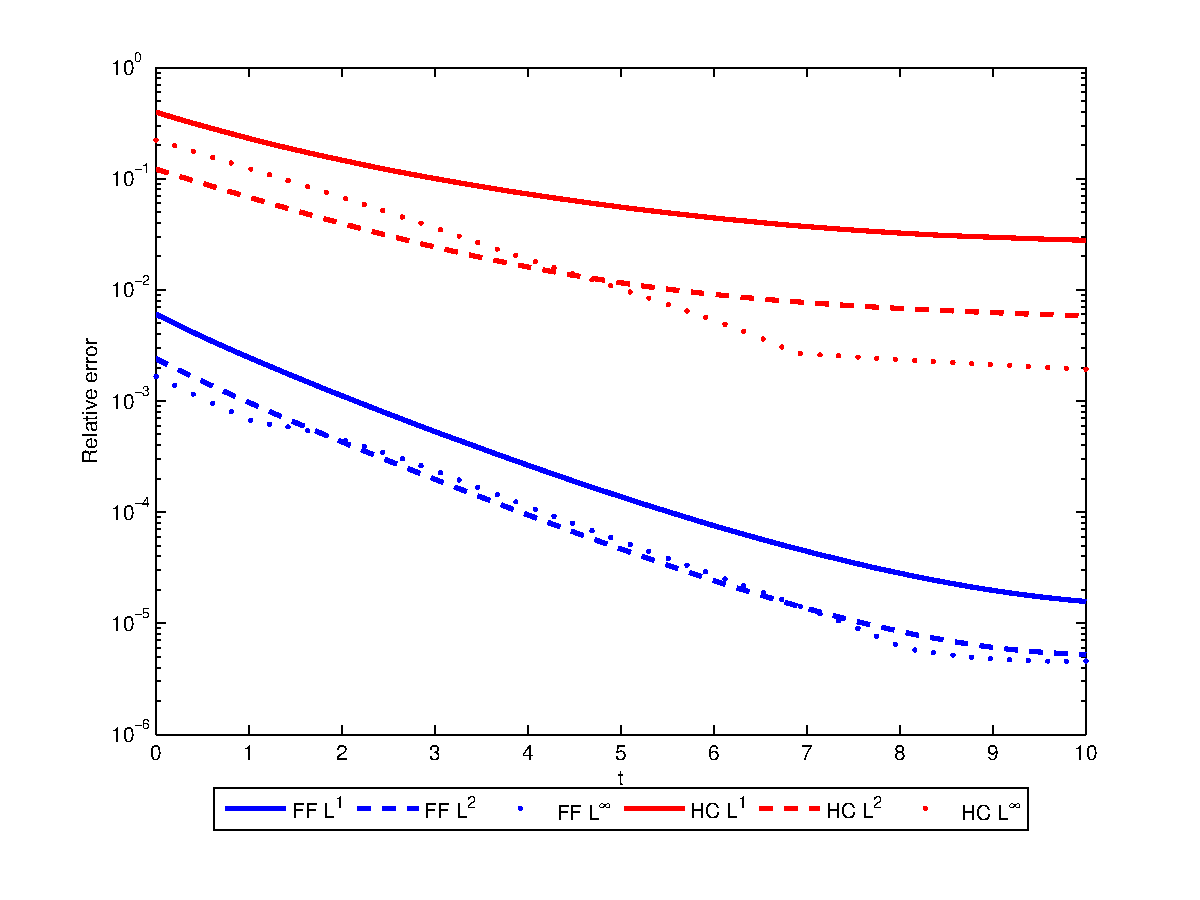
\includegraphics[width=11cm, height=7cm]{figs/hcboltz/bkwtime}
        \label{fig:bkw:time}
    }\\
    \subfloat[Relative error w.r.t. degrees of freedom at time $t=5.1$.]{
        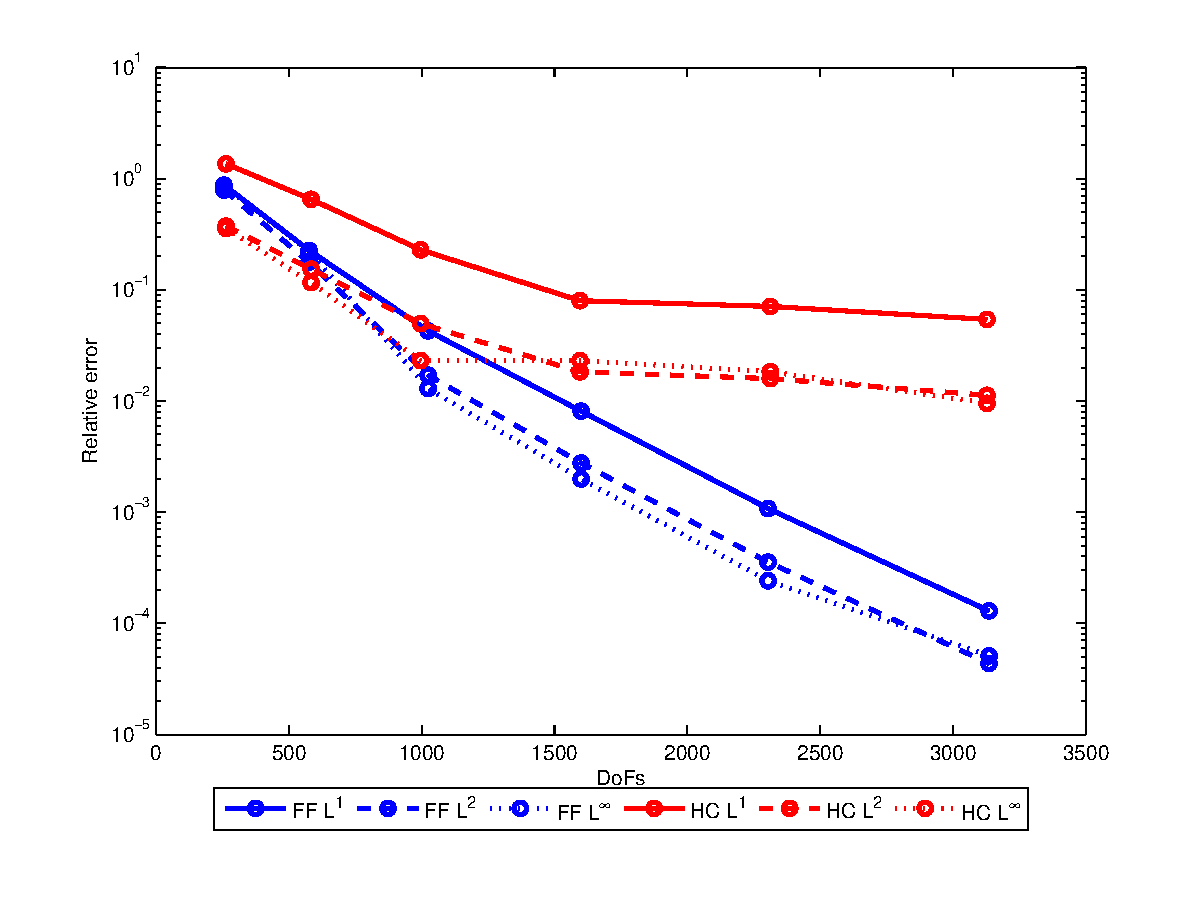
\includegraphics[width=11cm, height=7cm]{figs/hcboltz/bkw5-1}
        \label{fig:bkw:5.1}
    }
    \caption{Relative errors for the BKW solution for the full grid and hyperbolic cross methods, in $L^1$-,
    $L^2$- and $L^\infty$-norms. For timestepping, we used a fixed-timestep explicit 4\textsuperscript{th}
    order Runge-Kutta method with timestep $10^{-2}$. See Section~\vref{sec:verify} for details.}
    \label{fig:bkw} 
\end{figure}

Figure~\vref{fig:bkw} shows the results for this experiment. Note the poor approximation properties due to the
very narrow support of $f_0$, as well as the poor performance of the hyperbolic cross, due to the rotational
symmetry.  Note also how inaccurate initial data can still yield accurate long-term solutions. The solutions
themselves are shown in Figure~\vref{fig:bkw:sols}. Finally, Figure~\vref{fig:entropy} shows, for $N=56$, how
the entropy of the solution, 
\[ -\int_{\cD_L} f(\Bv)\log f(\Bv) \dd \Bv \] 
converges to the theoretical maximum as given by the equilibrium distribution.

\begin{figure}
    \centering
    \subfloat[Initial distribution.]{
        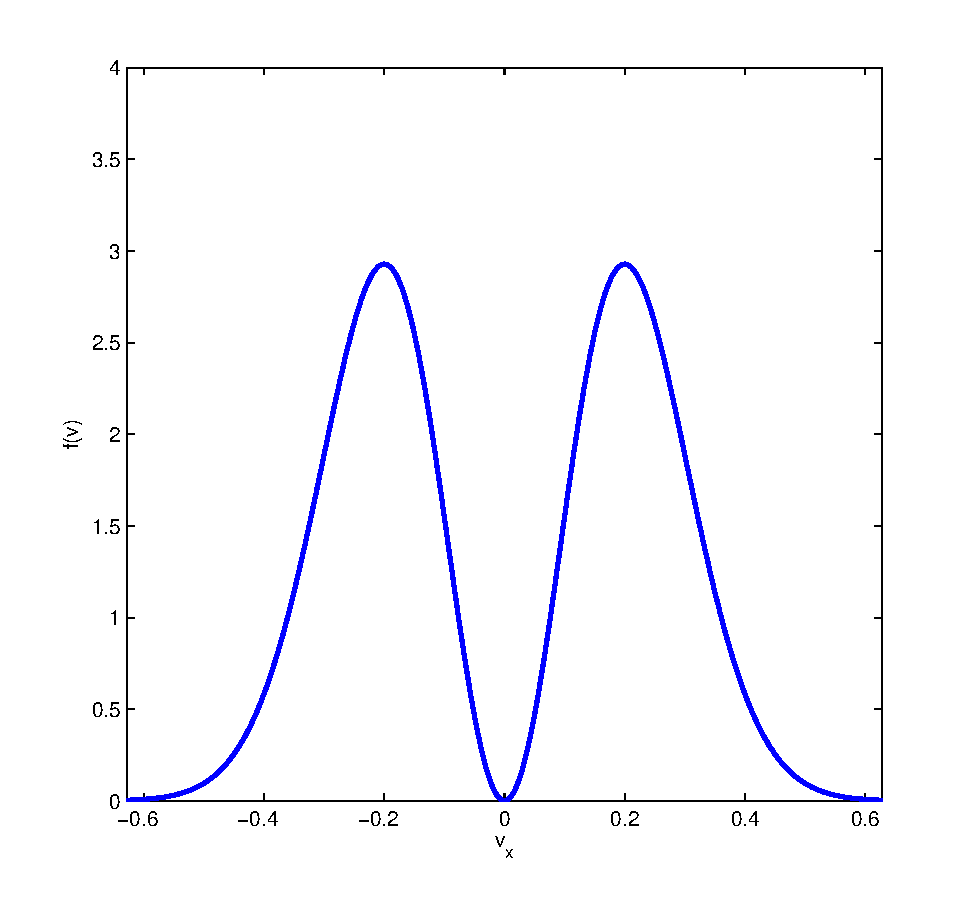
\includegraphics[width=6.45cm,height=6cm]{figs/hcboltz/bkwstart}
        \label{fig:bkw:start}
    }
    \subfloat[Equilibrium.]{
        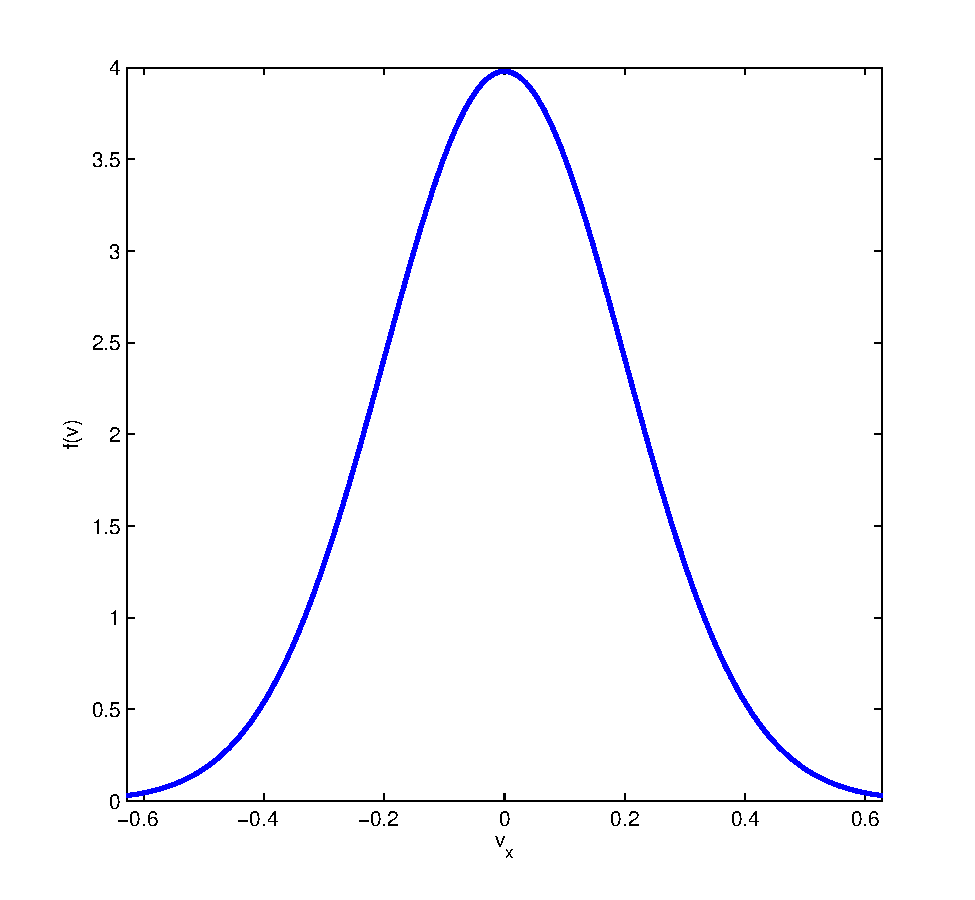
\includegraphics[width=6.45cm,height=6cm]{figs/hcboltz/bkweq}
        \label{fig:bkw:eq}
    }
    \caption{Cross-section plots of the BKW solution. Rotational symmetry applies. See
    Section~\vref{sec:verify} for details.}
    \label{fig:bkw:sols}
\end{figure}

\begin{figure}
    \centering
    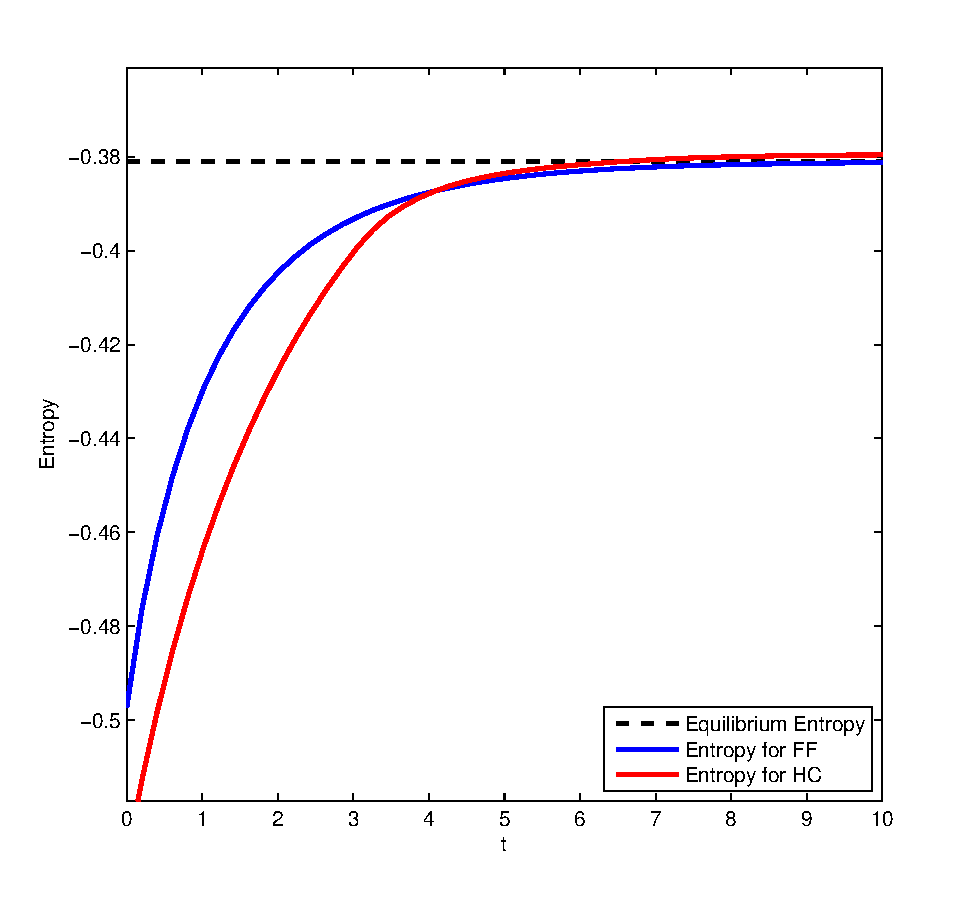
\includegraphics[width=7cm]{figs/hcboltz/entropy}
    \caption{Convergence of entropy for $\AFF(56)$ (correct) and $\cA_0(234)$ (incorrect) for the BKW
    solution. See Section~\vref{sec:verify} for details.}
    \label{fig:entropy}
\end{figure}

\clearpage

\subsection{Crossed streams} \label{sec:crossed}

This is an example of a case where the hyperbolic cross approximation works
very well. The initial condition is 
\[
    f_0(\Bv) = \left[(1+\sin(sv_x))e^{-sv_x^2} + 
            (1+\sin(sv_y))e^{-sv_y^2}\right] e^{-2|\Bv|^2}.
\]
There parameter $s>0$ can be tweaked to make $f_0$ more or less isotropic.  For
our experiment we have used $s=10$, and a hyperbolic cross with standard
fatness $T=0$.  We computed the solution over four time units, with an explicit
4\textsuperscript{th} order Runge-Kutta method with timestep $5\cdot10^{-3}$.

Since this is beyond the scope of known analytic solutions, we used a reference
solution computed on a full grid with $N=80$. The results for global
$L^2$-errors are shown in Figure~\vref{fig:hc1:l2}, and for observables in
Figure~\vref{fig:hc1:obs}.

In these cases, the hyperbolic cross can be seen to outperform the full grid
method, although the latter catches up over time and eventually wins out as the
solution approaches equilibrium, see Figure~\vref{fig:hc1:l2:time}.

\begin{figure}
    \centering
    \subfloat[Relative error at time $t=0$.]{
        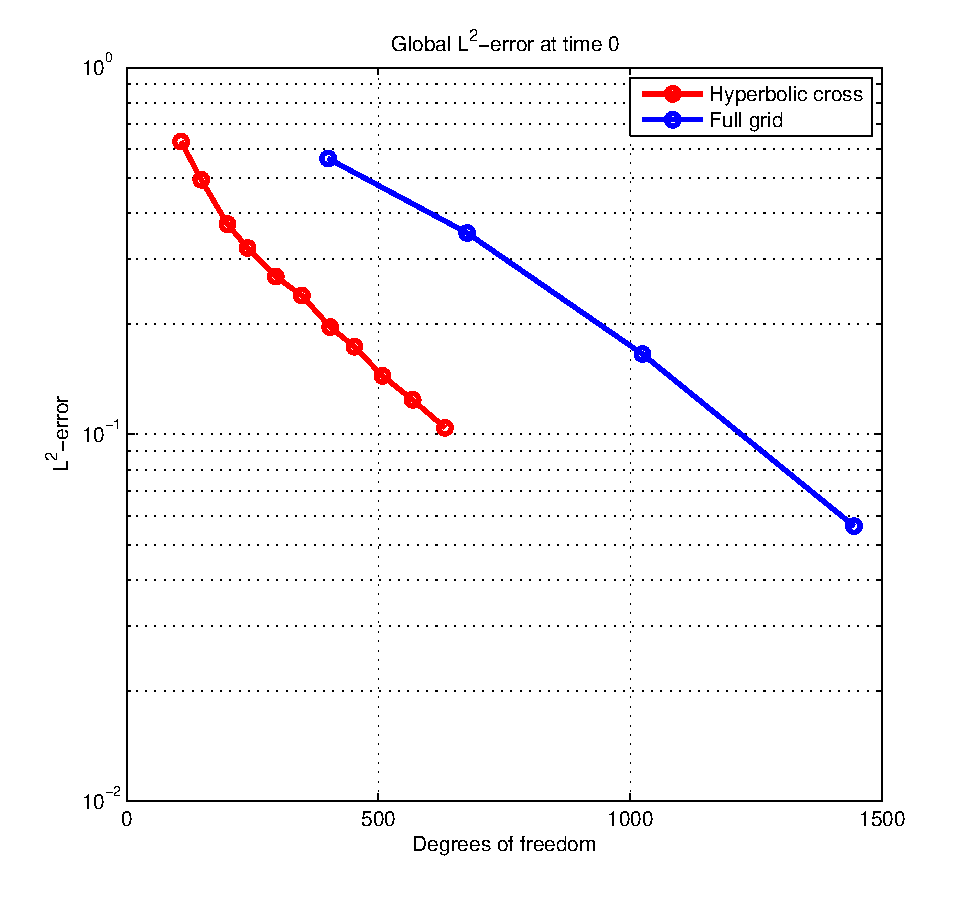
\includegraphics[width=6.8cm]{figs/hcboltz/hc1-l2-1}
        \label{fig:hc1:l2:1}
    }
    \hspace{-1.5cm}
    \subfloat[Relative error at time $t=0.96$.]{
        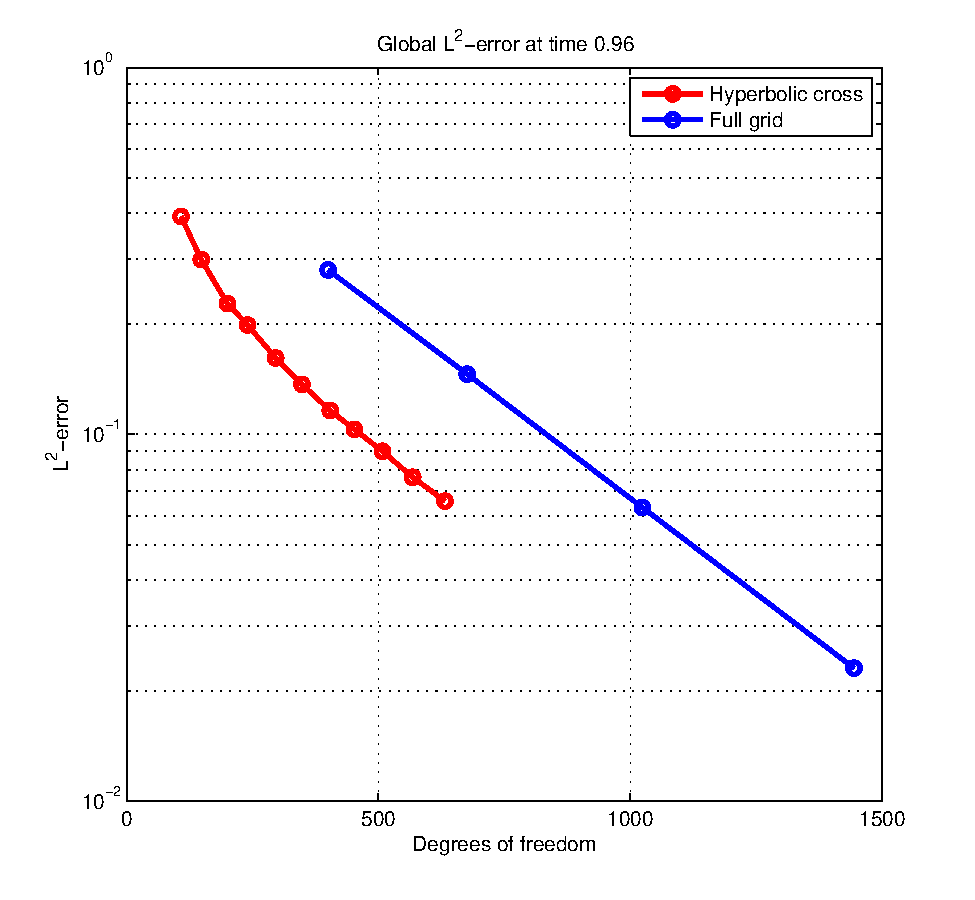
\includegraphics[width=6.8cm]{figs/hcboltz/hc1-l2-2}
        \label{fig:hc1:l2:2}
    }
    \\
    \subfloat[Relative error at time $t=2$.]{
        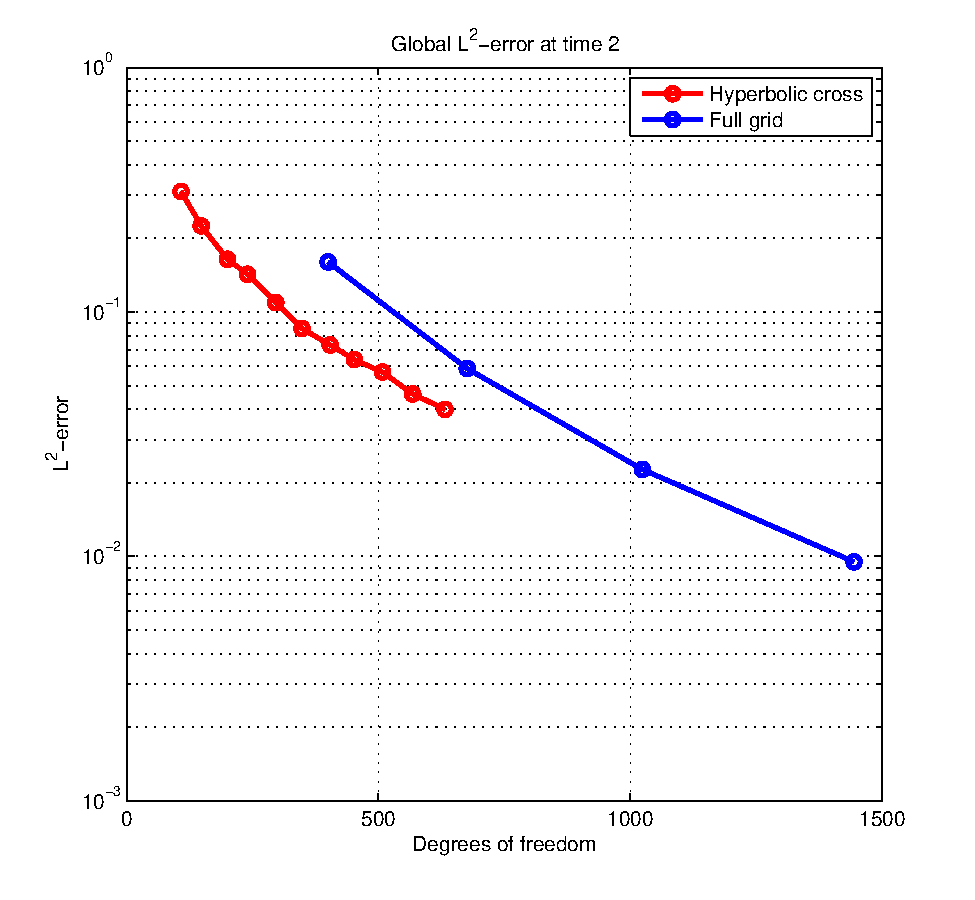
\includegraphics[width=6.8cm]{figs/hcboltz/hc1-l2-3}
        \label{fig:hc1:l2:3}
    }
    \hspace{-1.5cm}
    \subfloat[Relative error over time for $676$ and $632$ degrees of freedom, respectively.]{
        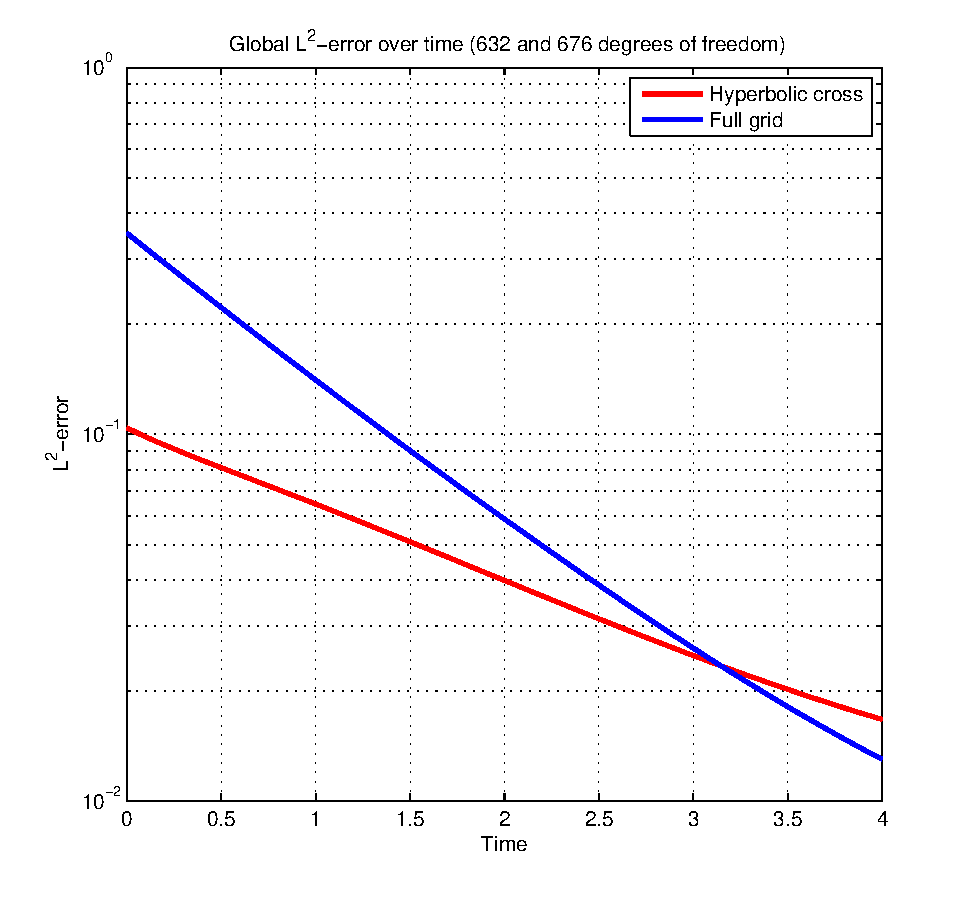
\includegraphics[width=6.8cm]{figs/hcboltz/hc1-l2-time}
        \label{fig:hc1:l2:time}
    }
    \caption{Relative $L^2$-errors for the crossed streams experiment. See Section~\vref{sec:crossed} for
    details.}
    \label{fig:hc1:l2}
\end{figure}

\begin{figure}
    \centering
    \subfloat[Error in observables at time $t=0$.]{
        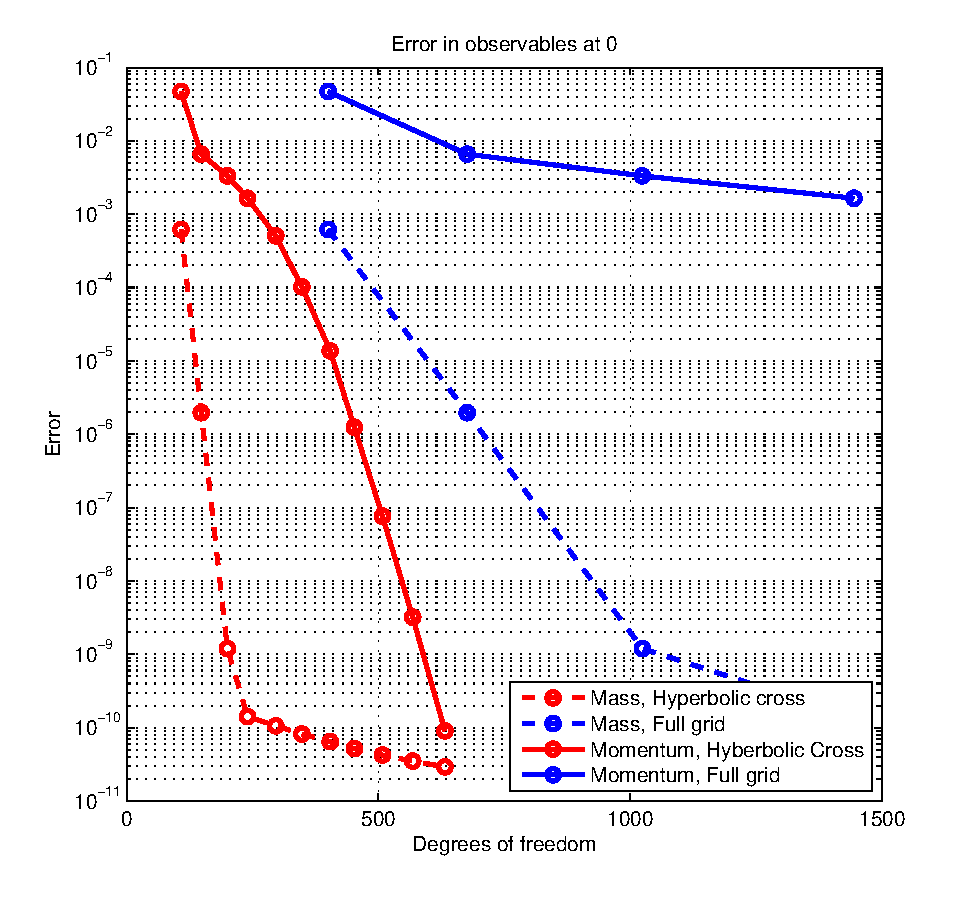
\includegraphics[width=7cm]{figs/hcboltz/hc1-obs-1}
        \label{fig:hc1:obs:1}
    }
    \subfloat[Error in observables at time $t=2$.]{
        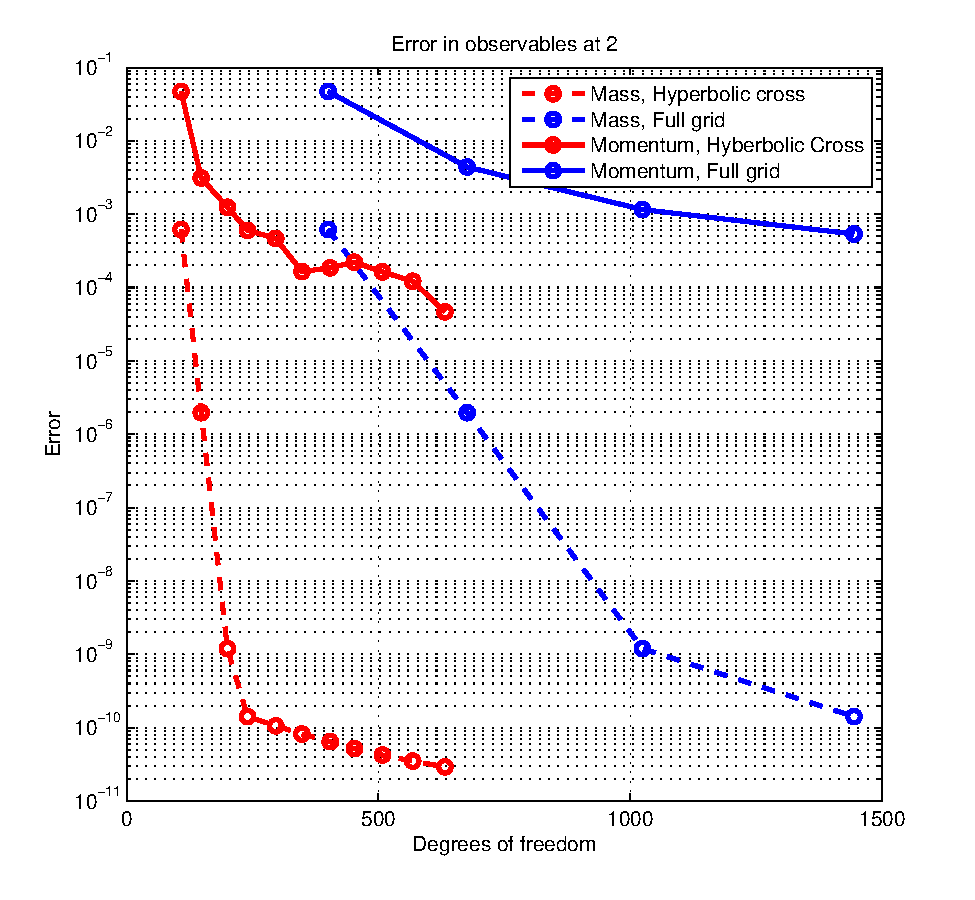
\includegraphics[width=7cm]{figs/hcboltz/hc1-obs-3}
        \label{fig:hc1:obs:3}
    }
    \caption{Errors in observables for the crossed streams experiment. See Section~\vref{sec:crossed} for
    details.}
    \label{fig:hc1:obs}
\end{figure}

\begin{figure}
    \centering
    \subfloat[Initial distribution.]{
        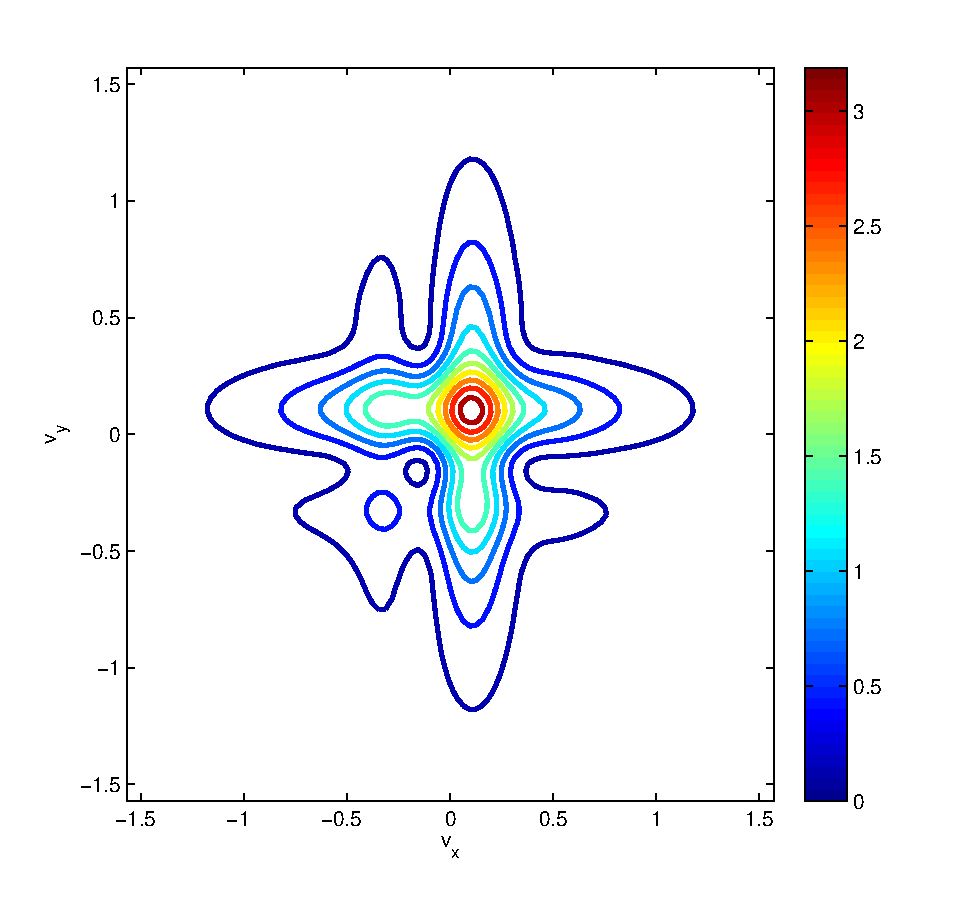
\includegraphics[width=6.45cm,height=5cm]{figs/hcboltz/crossed-1}
        \label{fig:hc1:start}
    }
    \subfloat[Solution at time $t=2$.]{
        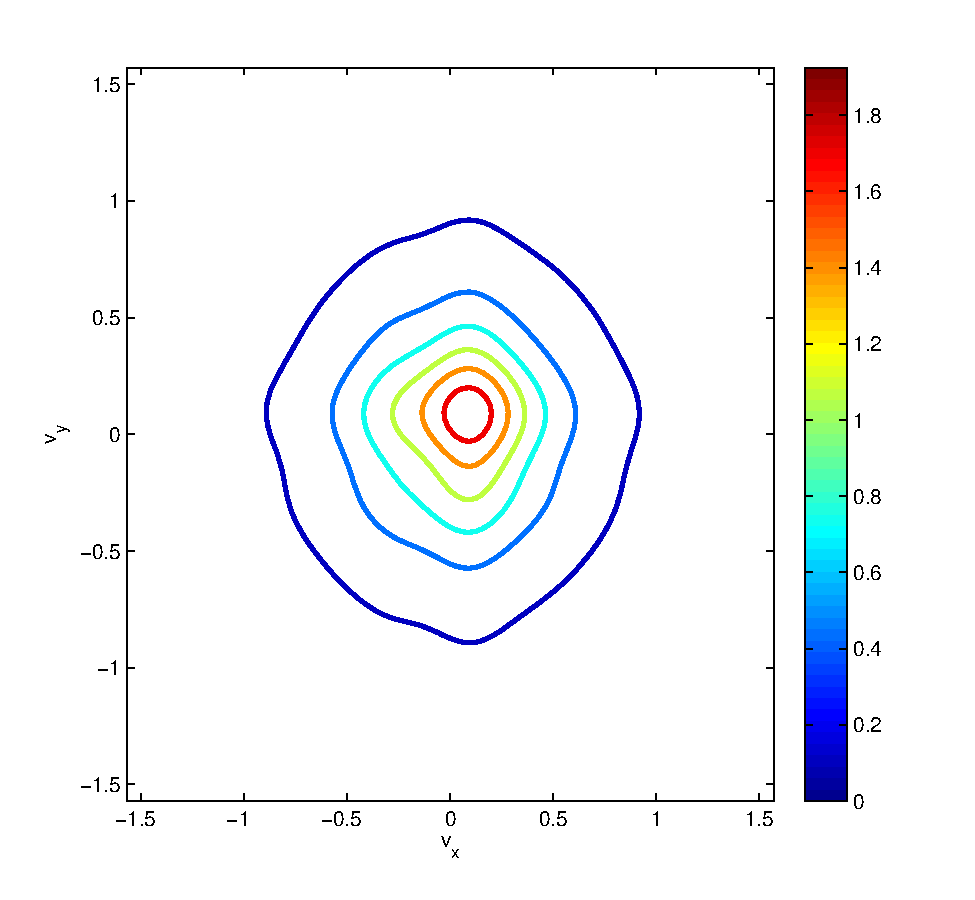
\includegraphics[width=6.45cm,height=5cm]{figs/hcboltz/crossed-3}
        \label{fig:hc1:eq}
    }
    \caption{The crossed streams solution. See Section~\vref{sec:crossed} for details.}
    \label{fig:hc1:sols}
\end{figure}

\subsection{Relaxation to equilibrium} \label{sec:relax}

This is an example of the offset method from Section~\ref{sec:offs}, using the initial distribution
\[
    f_0(\Bv) = e^{-2|\Bv|^2} + \epsilon\left(e^{-sv_x^2-v_y^2} + 
            e^{-v_x^2-sv_y^2}\right),
\]
where again the parameter $s>1$ controls the anisotropy of $f_{0}$, and
$\epsilon>0$ represents the fact that $f_0$ is a minor perturbation from
equilibrium.\footnote{Note that equilibrium is {\em not} $e^{-2|\Bv|^2}$ ---
the perturbation adds both mass density and temperature.}

Using $s=7$ and $\epsilon=10^{-2}$, we have plotted $\|f^p\|$ from \eqref{eq:fp}
versus time for three different norms in Figure~\vref{fig:relaxation}. The
convergence halts at $\|f^p\|\approx10^{-5}$ due to truncation error in $\Bv$ for
all norms, but prior to this, exhibits behavior in accordance with
\cite{Gressman11}.

\begin{figure}
    \centering
    \includegraphics[width=10cm]{figs/hcboltz/ds-pertnorms}
    \caption{Relaxation to equilibrium (see Section~\vref{sec:relax} for details):
      norms of the perturbation of the offset method versus time.} 
    \label{fig:relaxation}
\end{figure}

\subsection{Exponential decay of the numerical solution} \label{sec:decay}

We will here provide some numerical evidence that a certain exponential decay
can be expected to hold for the numerical solution using both $\AFF(N)$ and
$\cA_0(N)$ with some unspecified dependence $N=N(L)$. The decay we are after is
the existence of some $C$ independent of $L$ so that
\[
    \|f_{\cA(L)} \mu_a^{-1}\|_{L^2(\cD_L)} \leq C L^{\nicefrac{d}{2}}
\]
where $\mu_a$ is a Maxwellian with some decay rate $a$,
\[
    \mu_a(\Bv) = e^{-a|\Bv|^2}.
\]
This might go some way towards justifying Conjecture~\ref{ass:decay}. Note that the dependence on $L$ on the
right hand side is necessary in the limit $f_{\cA(L)} \to \mu_a$.

Table~\vref{tbl:numbers} shows these norms for various $N$ and $L$. For the $L$
chosen, a stable result of $\|f_{\cA(L)} \mu_a^{-1}\|_{L^2(\cD_L)}
\approx 1.3$ was achieved with relatively modest numbers of degrees of freedom.

A test with large values of $L$ would be difficult to perform with the current 
implementation, as the exponential weight at the boundaries of $\cD_L$ is much
larger than machine precision, artificially inflating the norms.

\begin{table}
\centering
\subfloat[$\AFF$]{
    \def\arraystretch{1.2}
    \begin{tabular}{c|c c c}
    $N$ & $L=0.5\pi$ & $L=0.75\pi$ & $L=\pi$ \\
    \hline 12 & 1.25 & 1.25 & 299  \\
    16 & 1.25 & 1.25 & 1.74 \\
    20 & 1.25 & 1.25 & 1.28 \\
    24 & 1.25 & 1.25 & 1.28 \\
    28 & 1.25 & 1.25 & 1.28 \\
    \end{tabular}
} \\
\subfloat[$\cA_0$]{
    \def\arraystretch{1.2}
    \begin{tabular}{c|c c c}
    $N$ & $L=0.5\pi$ & $L=0.75\pi$ & $L=\pi$ \\
    \hline 50 & 1.25 & 1.30 & $5.25\cdot10^4$ \\
    70 & 1.25 & 1.25 & $5.67\cdot10^3$ \\
    90 & 1.25 & 1.25 & $1.15\cdot10^3$ \\
    110 & 1.25 & 1.25 & 193 \\
    130 & 1.25 & 1.25 & 10.5 \\
    150 & 1.25 & 1.25 & 1.99 \\
    170 & 1.25 & 1.25 & 1.29 \\
    190 & 1.25 & 1.25 & 1.28 \\
    \end{tabular}
}
\caption{
    Numerical evidence for the exponential decay of $f_\cA$ (see Section~\vref{sec:decay} for details).
    The table shows $\sup_t\|f_\cA \mu_a^{-1}\|_{L^2(\cD_L)}$ for various $N$ and $L$. The test case
    was the crossed streams setup from Section~\vref{sec:crossed}, and integrated until $T=10$.
}
\label{tbl:numbers}
\end{table}

\subsection{Aliasing and anti-aliasing} \label{sec:aliasing}

The ratio $\kappa=\nicefrac{R}{L}$ can be adjusted to control aliasing between
different periods of the numerical solution. A small choice of $\kappa$ will
avoid aliasing for several timesteps, while a large choice will allow all
possible collisions to be treated in a single timestep.

The following Figures show the evolution for the BKW solution using $N=32$
degrees of freedom in each direction using a full Fourier grid over the time
interval $[0,10]$.

The initial and final distribution for $\kappa=\frac{2}{3+\sqrt{2}}\approx
0.45$ is shown in Figure~\vref{fig:r:normal}. It is clear that the solution
maintains its equilibrium very well due to the low aliasing.

\begin{figure}
    \centering
    \subfloat[Initial distribution.]{
        \includegraphics[width=6.8cm]{figs/hcboltz/bkw-r-normal-init}
        \label{fig:r:normal:init}
    }
    \subfloat[Solution at time $t=40$.]{
        \includegraphics[width=6.8cm]{figs/hcboltz/bkw-r-normal-end}
        \label{fig:r:normal:end}
    }
    \caption{Initial and final discrete solution for the BKW experiment using $\kappa\approx0.45$. Compare to
    Figure~\vref{fig:r:sqrt2}. Note the $y$-axis scales.}
    \label{fig:r:normal}
\end{figure}

\begin{figure}
    \centering
    \includegraphics[width=6.8cm]{figs/hcboltz/bkw-r-sqrt2-end}
    \caption{Solution at time $t=0.6$ for the BKW experiment using $\kappa=\sqrt{2}$. Compare to
    Figure~\ref{fig:r:normal}. Note the $y$-axis scales.}
    \label{fig:r:sqrt2}
\end{figure}

In \cite{Filbet11}, time-global consistency and convergence is shown under
various assumptions, one of which is $\kappa\geq\sqrt{2}$. The distribution for
this scheme at $t=0.6$ is shown in Figure~\vref{fig:r:sqrt2}. This time is well
before equilibrium is reached, and the effect of significant aliasing can be
seen. The solution is clearly nonphysical.

Figure~\vref{fig:testr} shows the time-evolution of the $L^2$-error for the BKW
solution for various $\kappa$, ranging from $0.45$ to $\sqrt{2}$. For long
times, the error will always tend toward $0.9935$, which happens to be the
$L^2$-norm between the physical equilibrium solution (the Maxwellian), and the
numerical equilibrium solution (a constant function). We observe that for large
$\kappa$, the numerical solution collapses to a constant very rapidly, and for
smaller $\kappa$, the solution remains qualitatively correct for much longer
times.

\begin{figure}
    \centering
    \includegraphics[width=10cm]{figs/hcboltz/testr}
    \caption{$L^2$-error versus time for the BKW solution at various $\kappa$. See the discussion in
    Section~\vref{sec:aliasing} for details.}
    \label{fig:testr}
\end{figure}

\cleardoublepage

\chapter{Homogeneous Boltzmann equation: polar spectral scheme}
\chaptermark{HBE: polar spectral scheme}
\label{chap:boltzmann-polar}

\section{Introduction} 
\label{sect:polar-intro}

Another idea, parallel to the Fourier discretization of Chapter~\ref{chap:boltzmann-fourier} is to discretize
$f$ in two dimensions using a polar coordinate representation
\[
    f(\Bv) = \sum_{k,l} F_{k,l} \varphi_k(r) \xi_l(\theta),
\]
where the angular modes $\xi$ are ordinary complex exponentials, and the radial modes $\varphi$ are
exponentially weighted Laguerre polynomials. This has been done previously, but only for radially symmetric
solutions (i.e. no dependence on $\theta$, see for example \cite{Ender94} and \cite{Ender99}, the former
appears unavailable in English). The present work features, to the best of our knowledge, the first
development of a polar scheme for general solutions.

This method is invariably more expensive per degree of freedom than the Fourier spectral discretization, since
there is no analogue of Theorem~\ref{thm:trans-rot-Q} in the radial direction. In return, it is possible to
resolve the equilibrium solution exactly. This method will also not be affected by the aliasing that can
plague the Fourier discretization, it requires no artificial truncation, and it can be made fully conservative
for all conserved moments.

\textbf{Outline.} In Section~\ref{sec:polar} we develop the details of the polar discretization. The form of
the basis functions are motivated, and existing error estimates for stationary functions are presented (though
no attempt is made to provide time-dependent estimates). In Section~\ref{sec:polar-equilibria}, we highlight
some of the most important aspects of the method, including its expected sparsity for long times and the
conservative properties. Section~\ref{sec:polar-evaluating} explains some issues with regards to
implementation and the tricks we used to speed up the code. Finally, numerical results are presented in
Section~\ref{sec:numerical-pol} for the polar method alone, and in Section~\ref{sec:numerical-fou-pol} we
attempt to compare the Fourier and the polar methods directly.

\section{The polar Laguerre function space} \label{sec:polar}

In the following chapter we will develop a polar spectral discretization for \eqref{eqn:boltzmann-sphom}. This
method will only be developed for $d=2$, but we will point out the work required to extend it to arbitrary
dimensions where applicable.

For the sake of simplicity of notation we will identify $\bbR^2$ with $\bbC$, and its standard polar
representation,
\[
    \Bv = x(\Bv) + \ii y(\Bv) = r(\Bv) \ee^{\ii\arg\Bv}.
\]
It will also be useful to use $\mu$ to denote a specific Maxwellian, instead of more general ones as before,
\begin{equation} \label{eqn:norm-max}
    \mu(\Bv) = \mu(r) = \ee^{-r^2}.
\end{equation}

Let us now define, for $l\in\bbZ$, $k\in\bbZ_{\geq0}$, $\beta>0$
\begin{align}
    \xi_l : \quad [0,2\pi) \to \bbC \quad &: \quad \theta \mapsto \ee^{\ii l \theta}, \label{eqn:def-ce} \\
    \psi_{k,\beta}^\rmS : \quad [0,\infty) \to \bbR \quad &: 
        \quad r \mapsto \ee^{-\nicefrac{r^2}{\beta}} L_k^{(0)}(r^2), 
    \label{eqn:def-psis} \\
    \psi_{k,\beta}^\rmK : \quad [0,\infty) \to \bbR \quad &: \quad r \mapsto \frac{1}{\sqrt{k+1}}
                                                 \ee^{-\nicefrac{r^2}{\beta}} r L_k^{(1)}(r^2).
    \label{eqn:def-psik}
\end{align}
Here, $L_k^{(\alpha)}$ denote the generalized Laguerre polynomials\footnote{Often called {\em associated}
Laguerre polynomials or {\em Sonine} polynomials} of order $\alpha$. They are defined as
\begin{equation} \label{eqn:def-lag}
    L_k^{(\alpha)}(x) = \sum_{i=0}^k (-1)^k \binom{k+\alpha}{k-i} \frac{x^i}{i!},
\end{equation}
and satisfy the recurrence relations
\begin{align} 
    \label{eqn:lag0-rec} (k+1)L^{(0)}_{k+1}(x) &= (2k+1-x)L_k^{(0)}(x) - kL_{k-1}^{(0)}(x), \qquad k \geq 1, \\
    \label{eqn:lag1-rec} L_k^{(\alpha+1)}(x) &= \sum_{i=0}^k L_i^{(\alpha)}(x),
\end{align}
with $L_0^{(0)} = 1$ and $L_1^{(0)} = 1-x$. The first few polynomials of order $0$ and $1$ are tabulated in
Table~\ref{tbl:laguerre} and plotted in Figure~\ref{fig:laguerre}.

\begin{table}
\centering
\def\arraystretch{1.4}
\begin{tabular}{c@{\qquad}r@{\qquad}r}
$k$ & $L_k^{(0)}$ & $L_k^{(1)}$ \\
\hline 0 & $1$ & $1$ \\
\hline 1 & $-x+1$ & $-x+2$ \\
\hline 2 & $\frac{1}{2}x^2 - 2x + 1$ & $\frac{1}{2}x^2 - 3x + 3$ \\
\hline 3 & $-\frac{1}{6}x^3 + \frac{3}{2}x^2 - 3x + 1$ & $-\frac{1}{6}x^3 + 2x^2 - 6x + 4$ \\
\hline 4 & $\frac{1}{24}x^4-\frac{2}{3}x^3+3x^2-4x+1$ & $\frac{1}{24}x^4-\frac{5}{6}x^3+5x^2-10x+5$ \\
\end{tabular}
\caption{The first few generalized Laguerre polynomials of order $0$ and $1$.} \label{tbl:laguerre}
\end{table}

\begin{figure}
\centering
\subfloat[Order $0$]{\includegraphics[width=10cm]{figs/polboltz/laguerre0}} \\
\subfloat[Order $1$]{\includegraphics[width=10cm]{figs/polboltz/laguerre1}}
\caption{The first six generalized Laguerre polynomials of order $0$ and $1$.}
\label{fig:laguerre}
\end{figure}

The polynomials $L_k^{(\alpha)}$ are orthogonal with respect to the weight $\ee^{-x}x^\alpha$: 
\begin{equation} \label{eqn:lag-orth}
    \int_0^\infty \ee^{-x}x^\alpha L^{(\alpha)}_k(x) L^{(\alpha)}_l(x) \dd x 
    = \binom{k+\alpha}{k} \Gamma(\alpha + 1) \delta_{k,l}.
\end{equation}
This is the motivation for the definitions \eqref{eqn:def-psis} and \eqref{eqn:def-psik}. Substituting
$x=r^2$, we see that $\psi_{k,\beta}^{\rmS}$ and $\psi_{k,\beta}^{\rmK}$ are orthogonal with respect to the
measure
\[
    \ee^{-(1-\nicefrac{2}{\beta})r^2} r \dd r,
\]
which fits with the volume element for polar integrals over $\bbR^2$. This will be made precise in the
following.

The functions $\psi_k^\rmS$ and $\psi_k^\rmK$ from \eqref{eqn:def-psis}, \eqref{eqn:def-psik} are
exponentially weighted polynomials of degree $2k$ and $2k+1$ containing only even and odd powers of $r$,
respectively. As such, it can be expected that if $f : [0,\infty) \to \bbR$ is analytic and sufficiently rapidly
decaying (a condition depending on $\beta$), and that its analytic extension to $\bbR$ is symmetric, it will
have an exponentially convergent representation in terms of the functions $\psi_{k,\beta}^\rmS$, and likewise
for $\psi_{k,\beta}^\rmK$ if $f$ has an anti-symmetric extension to $\bbR$.

\begin{proposition} \label{prop:szasz}
Let $f:[0,\infty)\to\bbR$ be given, and assume that $f$ has a symmetric analytic extension to the
strip $s(c) \defeq \left\{ z \;:\; |\Im z| \leq \sqrt{c} \right\}$ for some $c>0$, and that for every $b$ such
that $0 \leq b<c$, there exists $C(b)$ such that
\begin{equation} \label{eqn:sz-slowdecay}
    |f(z)| \leq C(b) \exp\left[\frac{x^2}{2} - |y|\left(b^2 - y^2\right)^{\frac{1}{2}}\right],
\end{equation}
for all $z = x + \ii y \in s(b)$. Then there exist convergent Laguerre series for $f$,
\[
    f(r) = \sum_{k=0}^\infty a^{(0)}_k L_k(r^2) = \sum_{k=0}^\infty a^{(1)}_k L^{(1)}_k(r^2),
\]
where the coefficients $a^{(\alpha)}_k$ for $\alpha\in\{0,1\}$ are given by
\[
    a^{(\alpha)}_k = \frac{1}{(k+1)^\alpha}\int_0^\infty \ee^{-x} x^\alpha L^{(\alpha)}_k(x)f(\sqrt{x})\dd x
\]
and satisfy the decay property
\[
    \big|a^{(\alpha)}_k\big| \leq 2 C(b) \ee^{-2b\sqrt{k}}.
\]
\end{proposition}
\begin{proof}
The existence of the Laguerre series is given by \cite[Theorem B]{Szasz58}.  By \cite[Lemma 3.4]{Szasz58} we
also conclude that for all $b$,
\[
    \big|a^{(0)}_k\big| \leq C(b) \ee^{-2b\sqrt{k}}.
\]
The corresponding decay for $a^{(1)}_k$ holds on account of the relation $a^{(1)}_k = a^{(0)}_k -
a^{(0)}_{k+1}$, which follows from Lemma \ref{lem:adecay}.
\end{proof}
\begin{lemma} \label{lem:adecay}
The Laguerre polynomials satisfy
\[
    xL^{(1)}_k(x) = (k+1)(L^{(0)}_k(x)-L^{(0)}_{k+1}(x)).
\]
\end{lemma}
\begin{proof}
We proceed by induction. As $L_0(x)=1$ and $L_1(x)=1-x$, the statement is evidently true for $k=0$. For the
induction step, we note that
\begin{align*}
    xL^{(1)}_k 
    & \quad \overset{\mathclap{\text{\eqref{eqn:lag1-rec}}}}{=} \quad
    xL^{(1)}_{k-1} + xL^{(0)}_k \\
    & \quad \overset{\mathclap{\text{IH}}}{=} \quad
    k(L^{(0)}_{k-1} - L^{(0)}_k) + xL^{(0)}_k \\
    & \quad \overset{\mathclap{\text{\eqref{eqn:lag0-rec}}}}{=} \quad
    k(L^{(0)}_{k-1} - L^{(0)}_k) + (2k+1)L^{(0)}_k - kL^{(0)}_{k+1} - (k+1)L^{(0)}_{k+1} \\
    & \quad = \quad (k+1)(L^{(0)}_k-L^{(0)}_{k+1}).
\end{align*}
This concludes the proof.
\end{proof}

Proposition \ref{prop:szasz} establishes the necessary conditions on a function $f$ to have rapidly decaying
Laguerre series approximations in terms of $L^{(\alpha)}(r^2)$ for $\alpha\in\{0,1\}$. We now consider
expansions of symmetric and anti-symmetric functions in terms of $\psi^\rmS$ and $\psi^\rmK$.

\begin{proposition} \label{prop:sz2}
Let $f^\rmS, f^\rmK: [0,\infty) \to \bbR$ be given. Assume that $f^\rmS$ and $\frac{1}{r}f^\rmK$ have analytic
symmetric extensions to the strip $s(c)$ for some $c>0$, and that for every $b$ such that $0\leq b<c$, there
exists $C(b)$ such that 
\begin{equation} \label{eqn:sz-fastdecay}
    |f^\rmS(z)|, \left|\frac{1}{z}f^\rmK(z)\right| \leq C(b) 
    \exp\left[-\frac{|z|^2}{\beta}+\frac{x^2}{2} - |y|\left(b^2 - y^2\right)^{\frac{1}{2}}\right],
\end{equation}
for all $z=x+\ii y \in s(b)$. Then there exist convergent series
\begin{equation} \label{eqn:prop-sz2-series}
    f^\rmS(r) = \sum_{k=0}^\infty a^\rmS_{k,\beta} \psi^\rmS_{k,\beta}(r), \qquad
    f^\rmK(r) = \sum_{k=0}^\infty a^\rmK_{k,\beta} \psi^\rmK_{k,\beta}(r),
\end{equation}
where, using $\mu$ as defined in \eqref{eqn:norm-max},
\begin{equation*}
    a^\rmS_{k,\beta} = \int_0^\infty \ee^{\nicefrac{x}{\beta}-x} L_k(x) f^\rmS(\sqrt{x}) \dd x 
             = 2\int_0^\infty \mu^{1-\nicefrac{2}{\beta}}(r) \psi^\rmS_{k,\beta}(r) f^\rmS(r) r \dd r \\
\end{equation*}
and
\begin{align*}
    a^\rmK_{k,\beta} 
        &= \frac{1}{\sqrt{k+1}} \int_0^\infty \ee^{\nicefrac{x}{\beta}-x} 
                        \sqrt{x} L^{(1)}_k(x) f^\rmK(\sqrt{x}) \dd x \\
        &= 2\int_0^\infty \mu^{1-\nicefrac{2}{\beta}}(r) \psi^\rmK_{k,\beta}(r) f^\rmK(r) r \dd r,
\end{align*}
and $|a^\rmS_{k,\beta}|, |a^\rmK_{k,\beta}| \leq 2C(b)\sqrt{k+1}\;\ee^{-2b\sqrt{k}}$.
\end{proposition}
\begin{proof}
It is clear that both $f^\rmS$ and $\frac{1}{r}f^\rmK$ are even and analytic. Moreover, on account of
\eqref{eqn:sz-fastdecay}, we see that the functions
\[
    \ee^{\nicefrac{r^2}{\beta}}f^\rmS(r),\qquad \ee^{\nicefrac{r^2}{\beta}}\frac{1}{r}f^\rmK(r)
\]
both satisfy the conditions of Proposition~\ref{prop:szasz}. Thus, we have
\[
    \ee^{\nicefrac{r^2}{\beta}} f^\rmS(r) = \sum_{k=0}^\infty a^\rmS_k L_k(r^2), \qquad
    \ee^{\nicefrac{r^2}{\beta}} \frac{1}{r} f^\rmK(r) = \sum_{k=0}^\infty \tilde{a}^\rmK_k L^{(1)}_k(r^2),
\]
which gives \eqref{eqn:prop-sz2-series} with $a^\rmK_k = \tilde{a}^\rmK_k\sqrt{k+1}$. The expressions for
$a^\rmS_k$ and $a^\rmK_k$ as well as their decay follow directly from Proposition~\ref{prop:szasz}.
\end{proof}
Let us now take the step to two dimensions, and consider an analytic function $f:\bbR^2\to\bbR$. Associated
with $f$ are its symmetric and anti-symmetric parts,
\[
    f^\rmS(r,\theta) = \frac{1}{2}\left(f(r,\theta) + f(r,\theta+\pi)\right), \qquad
    f^\rmK(r,\theta) = \frac{1}{2}\left(f(r,\theta) - f(r,\theta+\pi)\right),
\]
which are also both analytic. Fixing $\theta$ (effectively considering it as a parameter), and assuming that
$f^\rmS$ and $f^\rmK$ satisfy the conditions of Proposition~\ref{prop:sz2} for some $\beta>0$, we can write
\[
    f^\rmS(r,\theta) = \sum_{k=0}^\infty a^\rmS_{k,\beta}(\theta) \psi^\rmS_{k,\beta}(r), \qquad
    f^\rmK(r,\theta) = \sum_{k=0}^\infty a^\rmK_{k,\beta}(\theta) \psi^\rmK_{k,\beta}(r),
\]
where $a^\rmS$ and $a^\rmK$ are rapidly decaying in $k$.  In fact, as $f^\rmS$ is symmetric, we should be able
to approximate $a^\rmS_{k,\beta}(\theta)$ in terms of the complex exponentials $\xi_l$ (from
\eqref{eqn:def-ce}) for {\em even} $l$, and correspondingly $a^\rmK_{k,\beta}(\theta)$ in terms of $\xi_l$ for
{\em odd} $l$.

To simplify notation, let us introduce the functions
\[
    \varphi_k^{(\beta)} = \begin{cases} 
        \psi^\rmS_{\nicefrac{k}{2},\,\beta}, & k \equiv 0\; (\Mod 2), \\ 
        \psi^\rmK_{\nicefrac{(k-1)}{2},\,\beta}, & k \equiv 1\; (\Mod 2),
    \end{cases}
\]
so that we may write
\[
    f(r,\theta) = f^\rmS(r,\theta) + f^\rmK(r,\theta) = 
    \sum_{k=0}^\infty a_k^{(\beta)}(\theta) \varphi_k^{(\beta)}(r),
\]
where $a_k$ corresponds to $a^\rmS_{\nicefrac{k}{2},\,\beta}$ for even $k$ and to
$a^\rmK_{\nicefrac{(k-1)}{2},\,\beta}$ for odd $k$, and where $a_k$ has the same parity as $k$, i.e.
$a_k(\theta+\pi) = (-1)^k a_k(\theta)$.

Continuing from before, we now write
\[
    a_k^{(\beta)}(\theta) = \sum_{2\,|(k-l)} F_{k,l}^{(\beta)} \xi_l(\theta),
\]
where
\[
    F_{k,l}^{(\beta)} = \frac{1}{2\pi} \int_0^{2\pi} a_k^{(\beta)}(\theta) \xi_{-l}(\theta) \dd\theta.
\]
Let us first consider $k$ even. Then
\begin{align*}
    F_{k,l}^{(\beta)} &= \frac{1}{\pi} \int_0^{2\pi} \int_0^\infty \mu^{1-\nicefrac{2}{\beta}}
             \varphi_k^{(\beta)} \xi_{-l} f^\rmS \; r \dd r \dd\theta \\
          &= \frac{1}{\pi} \int_{\bbR^2} \mu^{1-\nicefrac{2}{\beta}} \varphi_k^{(\beta)} 
             \xi_{-l} f^\rmS \dd \Bv
           = \frac{1}{\pi} \int_{\bbR^2} \mu^{1-\nicefrac{2}{\beta}} \varphi_k^{(\beta)} 
             \xi_{-l} f \dd \Bv,
\end{align*}
since $\xi_{-l}$ is even, the corresponding integral with $f^\rmK$ will be zero. Precisely the same argument
applies for $k$ odd. As such, we arrive at
\begin{equation} \label{eqn:polexp}
    f(r,\theta) = \sum_{2\,|(k-l)} F_{k,l}^{(\beta)} \; \varphi_k^{(\beta)} (r) \xi_l(\theta),
\end{equation}
where the notation $a|b$ is understood to mean that $a$ divides evenly into $b$. The coefficients are given by
\[
    F_{k,l}^{(\beta)} = \frac{1}{\pi} \int_{\bbR^2} \mu^{1-\nicefrac{2}{\beta}} 
                        \varphi_k^{(\beta)} \xi_{-l} f \dd\Bv.
\]
This implies that the functions $\varphi_k^{(\beta)}\xi_l$ form an orthogonal system with respect to the
weight $\mu^{1-\nicefrac{2}{\beta}}$. This is in fact the case, and it is not difficult to see.
\begin{proposition} \label{prop:orthopol}
Assuming $k_1 \equiv l_1\;(\Mod2)$ and $k_2\equiv l_2\;(\Mod2)$, we have
\[
    \left\langle \varphi_{k_1}^{(\beta)} \xi_{l_1}, \varphi_{k_2}^{(\beta)} \xi_{l_2} 
    \right\rangle_{L^2(\bbR^2;\,\beta)} 
    = \int_{\bbR^2} \mu^{1-\nicefrac{2}{\beta}} 
      \varphi_{k_1}^{(\beta)} \xi_{l_1} \varphi_{k_2}^{(\beta)} \xi_{-l_2} \dd\Bv
    = \pi \delta_{k_1,k_2} \delta_{l_2,l_2}.
\]
\end{proposition}
\begin{proof}
First, we note that if $k_1$ and $k_2$ have different parities, the integrand in question is odd, so the
integral is zero. Thus, we assume from now that they have equal parities. We have
\begin{align*}
    \left\langle \varphi^{(\beta)}_{k_1}\xi_{l_1}, \varphi^{(\beta)}_{k_2}\xi_{l_2} 
    \right\rangle_{L^2(\bbR^2;\,\beta)} 
    &= \int_0^{2\pi} \xi_{l_1-l_2} \dd\theta \int_0^\infty \mu^{1-\nicefrac{2}{\beta}}
       \varphi_{k_1}^{(\beta)} \varphi_{k_2}^{(\beta)}\; r \dd r \\
    &= 2\pi\delta_{l_1,l_2} \int_0^\infty \mu^{1-\nicefrac{2}{\beta}}
       \varphi_{k_1}^{(\beta)} \varphi_{k_2}^{(\beta)} \;r \dd r. \\
\end{align*}
For $k_1, k_2$ both even, we have
\begin{align*}
    \int_0^\infty \mu^{1-\nicefrac{2}{\beta}} \varphi_{k_1}^{(\beta)} \varphi_{k_2}^{(\beta)} r \dd r
    &= \int_0^\infty \ee^{-r^2} L_{\nicefrac{k_1}{2}}(r^2) L_{\nicefrac{k_2}{2}}(r^2)\; r \dd r \\
    &= \frac{1}{2} \int_0^\infty \ee^{-x} L_{\nicefrac{k_1}{2}}(x) L_{\nicefrac{k_2}{2}}(x) \dd x
    \overset{\text{\eqref{eqn:lag-orth}}}{=} \frac{1}{2} \delta_{k_1,k_2}.
\end{align*}
And for $k_1, k_2$ both odd, we find, using $Z(a,b)=[(a+1)(b+1)]^{-\nicefrac{1}{2}}$,
\begin{align*}
    \int_0^\infty \mu^{1-\nicefrac{2}{\beta}} \varphi_{k_1}^{(\beta)} \varphi_{k_2}^{(\beta)} r \dd r
    &= 2Z(k_1,k_2) \int_0^\infty
       \ee^{-r^2} r^2 L^{(1)}_{\nicefrac{(k_1-1)}{2}}(r^2) L^{(1)}_{\nicefrac{(k_2-1)}{2}}(r^2)\; r \dd r \\
    &= Z(k_1,k_2) \int_0^\infty 
       \ee^{-x} x L^{(1)}_{\nicefrac{(k_1-1)}{2}}(x) L^{(1)}_{\nicefrac{(k_2-1)}{2}}(x) \dd x \\
    & \overset{\text{\eqref{eqn:lag-orth}}}{=} \frac{1}{2} \delta_{k_1,k_2}.
\end{align*}
This concludes the proof.
\end{proof}
We will use the notation $L^2(\bbR^2;\,\beta)$ to denote the weighted space in which the orthogonality holds,
with inner product
\[
    \langle f,g \rangle_{L^2(\bbR^2;\,\beta)} = \int_{\bbR^2} \mu^{1-\nicefrac{2}{\beta}} f g \dd\Bv.
\]
We also note in passing that $L^2(\bbR^2;\,2)=L^2(\bbR^2)$, that is, for $\beta=2$ we have orthogonality with
respect to the usual Lebesgue measure.

Thus, for $K,L,\beta>0$ and $L$ even, we define the finite-dimensional function spaces
\[ \boxed{
    \cV_\beta(K,L) = \spann \left\{ \varphi^{(\beta)}_k\xi_l \;:\; 0\leq k < K, \; -L \leq l < L, \;
    k \equiv l \;(\Mod 2) \right\}
} \]
of dimension $KL$, and we denote the implied basis by $\cB_\beta(K,L)$. The requirement that $L$ is even is
made purely for simplifying reasons, as the basis functions can then be enumerated as $b_{k,q} = \varphi_k
\xi_{l(q,k)}$ for $0 \leq k < K$ and $0 \leq q < L$, where
\begin{equation} \label{eqn:pol-enum}
    l(q,k) = \begin{cases} 2q - (-1)^k,& q < \nicefrac{L}{2} \\
                           2(q-L) - (-1)^k,& \text{otherwise}.
             \end{cases}
\end{equation}
Let us also denote by $P_{\cV_\beta(K,L)}$ (or, when convenient, merely $P_\cV$) the
$L^2(\bbR^2;\,\beta)$-orthogonal projection onto $\cV_\beta(K,L)$. Then, given an initial condition
$f_0(\Bv)$, we propose to solve \eqref{eqn:boltzmann-sphom} approximately through the projected equation
\[
    \frac{\partial f_\cV}{\partial t} = P_\cV Q(f_\cV,f_\cV), \qquad
    f_\cV(0) = P_\cV f_0.
\]
It is noteworthy that, unlike \eqref{eqn:boltzmann-nd}, there is no need to truncate the collision operator in
this case. In this way we also avoid all the aliasing effects which plague the Fourier methods.

\section{Equilibria and initial values}
\label{sec:polar-equilibria}

The space $\cV_\beta(K,L)$ contains functions on the form 
\[
    \varphi^{(\beta)}_0\xi_0 = \exp(-\nicefrac{|\Bv|^2}{\beta}),
\]
which are equilibrium solutions with mass density $\beta\pi$, momentum $\Bzero$ and temperature
$\nicefrac{\beta}{2}$. Thus, if the initial condition conforms to these conditions, we can expect that for
$k,l$ not both zero, the corresponding coefficient $F^{(\beta)}_{k,l}$ tends to zero.  If the initial
condition does not conform, the equilibrium solution cannot be exactly represented in any finite space
$\cV_\beta(K,L)$, but owing to the equilibrium solution being isotropic (if $\Bu=\Bzero$), it will certainly
still have a sparse representation. In this case, we expect $F^{(\beta)}_{k,l}$ to tend to zero for all
$l\neq0$.

\begin{definition} \label{def:conf}
    We say that a function $f(\Bv)$ is $\beta$-{\em conforming} if
    \[
        \rho(f) = \beta\pi, \qquad
        \Bu(f) = \Bzero, \qquad
        T(f) = \frac{\beta}{2}.
    \]
\end{definition}

\begin{theorem} \label{thm:trf-sols}
    Let $g(t,\Bv)$ be a solution to \eqref{eqn:boltzmann-sphom}, where $B$ satisfies Assumption~\ref{ass:B}.
    Let $\alpha,\gamma > 0$ be given, and define $\eta = \nicefrac{\alpha}{\gamma^{\lambda+2}}$. Then
    \[
        h(t,\Bv) = \alpha g(\eta t, \gamma \Bv)
    \]
    is also a solution to \eqref{eqn:boltzmann-sphom}.
\end{theorem}
\begin{proof}
    First,
    \begin{align*}
        \frac{\partial h}{\partial t}(t,\Bv)
        &= \alpha\eta \frac{\partial g}{\partial t}(\eta t, \gamma \Bv) \\
        &= \alpha\eta \int_{\bbR^2}\int_{\bbS^1} |\gamma\Bv-\overline{\Bv}_\ast|^\lambda b(\cos\theta) \\
        & \qquad\qquad\qquad\qquad
            \left[ g(\eta t,\overline{\Bv}') g(\eta t,\overline{\Bv}_\ast') -
                   g(\eta t,\gamma\Bv) g(\eta t,\overline{\Bv}_\ast) \right]
            \dd\Bsigma \dd\overline{\Bv}_\ast,
    \end{align*}
    where the collision identities read
    \[
        \overline{\Bv}', \overline{\Bv}_\ast' = \frac{1}{2}\left(
        \gamma\Bv+\overline{\Bv}_\ast \pm |\gamma\Bv-\overline{\Bv}_\ast|\Bsigma \right).
    \]
    Making the change of variables $\overline{\Bv}_\ast, \overline{\Bv}', \overline{\Bv}_\ast'
    = \gamma\Bv_\ast, \gamma\Bv', \gamma\Bv_\ast'$, we recover the familiar collision identity
    \[
        \Bv', \Bv_\ast' = \frac{1}{2}\left(
        \Bv+\Bv_\ast \pm |\Bv-\Bv_\ast|\Bsigma \right),
    \]
    whence
    \begin{align*}
        \frac{\partial h}{\partial t}(t,\Bv)
        &= \alpha\eta \int_{\bbR^2}\int_{\bbS^1} |\gamma\Bv-\gamma\Bv_\ast|^\lambda b(\cos\theta) \\
        & \qquad\qquad\qquad
            \left[ g(\eta t,\gamma\Bv) g(\eta t,\gamma\Bv_\ast') -
                   g(\eta t,\gamma\Bv) g(\eta t,\gamma\Bv_\ast) \right]
            \dd\Bsigma \dd(\gamma\Bv_\ast) \\
        &= \frac{\eta\gamma^{\lambda+2}}{\alpha} Q(h,h)(\Bv).
    \end{align*}
    Since $\nicefrac{\eta\gamma^{\lambda+2}}{\alpha}=1$, this concludes the proof.
\end{proof}
\begin{remark}
    A corresponding result to Theorem~\ref{thm:trf-sols} holds in arbitrary dimensions $d$, where
    $\eta=\nicefrac{\alpha}{\gamma^{\lambda+d}}$.
\end{remark}
The ``problem'' of nonconforming initial values is easily overcome. Theorem~\ref{thm:trf-sols} allows us to
transform any initial condition $f(0,\Bv)$ to conform to the space $\cV_\beta(K,L)$, solve it there, and then
recover the solution later, as demonstrated in the following theorem. This is important to the viability of
the method, since conformity can be maintained without assembling discrete collision operators for a variety
of different spaces with different values of observables.
\begin{theorem} \label{thm:conf-sols}
    Let $f(t,\Bv)$ be a solution to \eqref{eqn:boltzmann-sphom}, where $B$ satisfies Assumption~\ref{ass:B}.
    Let $\beta>0$ be given, and assume $f$ has mass density, momentum and temperature $\rho$, $\Bu$ and $T$. 
    Define
    \begin{equation} \label{eqn:poltrf}
        \gamma = \sqrt{\frac{2T}{\beta}}, \qquad
        \alpha = \frac{2\pi T}{\rho}, \qquad
        \eta   = \frac{\alpha}{\gamma^{\lambda+2}}.
    \end{equation}
    Then 
    \[
        h(t,\Bv)=\alpha f(\eta t, \gamma\Bv + \Bu)
    \]
    is a conforming solution to \eqref{eqn:boltzmann-sphom}, and $f$ can be recovered via $f(t,\Bv) =
    \alpha^{-1} h(\nicefrac{t}{\eta}, \nicefrac{(\Bv-\Bu)}{\gamma})$.
\end{theorem}
\begin{proof}
    We show that $h$ is conforming. Indeed,
    \begin{equation} \label{eqn:poltrf-mass}
        \rho(h) = \alpha\int_{\bbR^2} f(\gamma\Bv+\Bu) \dd\Bv 
        = \frac{\alpha}{\gamma^2}\int_{\bbR^2} f(\gamma\Bv+\Bu) \dd(\gamma\Bv+\Bu)
        = \frac{\alpha}{\gamma^2}\rho,
    \end{equation}
    and
    \begin{align}
        \nonumber T(h) &= \frac{1}{2\rho(h)} \int_{\bbR^2} \alpha f(\gamma\Bv+\Bu) \dd\Bv
        = \frac{1}{2\gamma^2\rho}\int_{\bbR^2} f(\Bs)|\Bs-\Bu|^2\dd\Bs \\
        \nonumber &= \frac{1}{2\gamma^2\rho}\left[ \int_{\bbR^2}f(\Bs)|\Bs|^2\dd\Bs +
           |\Bu|^2\int_{\bbR^2}f(\Bs)\dd\Bs - 2\Bu\cdot\int_{\bbR^2}f(\Bs)\Bs\dd\Bs\right] \\
        &= \frac{1}{2\gamma^2}\left[E + |\Bu|^2 - 2|\Bu|^2\right] = \frac{1}{\gamma^2}T.
        \label{eqn:poltrf-T}
    \end{align}
    Setting $\rho(h)=\beta\pi$ and $T(h)=\nicefrac{\beta}{2}$, and solving
    \eqref{eqn:poltrf-mass}-\eqref{eqn:poltrf-T} for $\alpha,\gamma$, we find precisely \eqref{eqn:poltrf}. It
    is easy to see that $\Bu(h)=\Bzero$. 
    
    It being a solution to \eqref{eqn:boltzmann-sphom} is an easy corollary of theorems \ref{thm:trans-rot-Q}
    and \ref{thm:trf-sols}.
\end{proof}

\subsection{Choice of $\beta$}

The properties of the bases $\cB_\beta$ depend rather heavily on the value of $\beta$. We have already noted
that for $\beta=2$, the weighted inner product $\langle\cdot,\cdot\rangle_{L^2(\bbR^2;\,\beta)}$ becomes the
usual $L^2$ inner product, and so error analysis in familiar norms will be simpler. In fact, one observes
that for most functions $f$, the coefficients $F_{k,l}^{(\beta)}(f)$ decay fastest for $\beta=2$, and one can
consistently achieve better error rates than $\beta<2$, both in the weighted norm and the $L^2$-norm.

On the other hand, we have the following Theorem concerning the stability of the bases with respect to the
observables.
\begin{theorem} \label{thm:polobs}
Let $\beta>0$ be given and define the linear functionals\footnote{Here we have abused notation somewhat, since
the quantity $(E\rho)(f)$ as defined is only equal to $E(f)\rho(f)$ if $\rho(f)\neq0$, and similarly for
$\Bu\rho$.}
\begin{gather*}
    \rho(f) = \int_{\bbR^2} f(\Bv) \dd\Bv, \qquad
    (\Bu \rho)(f) = \int_{\bbR^2} f(\Bv) \Bv \dd\Bv,\\
    (E \rho)(f) = \int_{\bbR^2} f(\Bv) |\Bv|^2 \dd\Bv.
\end{gather*}
Then,
\begin{align*}
    \rho\left(\xi_0\psi^\rmS_{k,\beta}\right) &= \beta\pi(1-\beta)^k, \\
    (\Bu\rho)\left(\xi_{\pm 1}\psi^\rmK_{k,\beta}\right) &= \frac{\beta^2\pi}{2}\sqrt{k+1}(1-\beta)^k
    \begin{pmatrix}1\\\pm1\end{pmatrix}, \\
    (E\rho)\left(\xi_0\psi^\rmS_{k,\beta}\right) &= 
        \begin{cases}
            \beta^2\pi[1-(k+1)\beta](1-\beta)^{k-1}, & k>0, \\
            \beta^2\pi, & k=0,
        \end{cases}
\end{align*}
using the convention that $0^0=1$ if $\beta=1$. For all other valid combinations of $\xi_l$ and
$\psi^\cdot_{k,\beta}$ the functionals evaluate to zero.
\end{theorem}
\begin{proof}
The proof for this is not difficult, but it involves a fair amount of algebra. First, we have the expansion of
Laguerre polynomials in terms of monomials,
\[
    L_k^{(\alpha)}(x) = \sum_{i=0}^k \binom{k+\alpha}{k-i} \frac{(-1)^i}{i!} x^i.
\]
For mass density and temperature, we first note that any integration against $\xi_l$ for $l\neq0$ must yield
zero. For momentum, note that (considering $\Bv$ as a complex number) we have $\Bv = \xi_1(\Bv) r$, so any
integration against $\xi_l$ for $l\neq-1$ must yield zero.

Thus, for mass density we have
\begin{align*}
\rho\left(\xi_0\psi^\rmS_{k,\beta}\right) 
&= 2\pi \int_0^\infty \ee^{-\nicefrac{r^2}{\beta}} L_k(r^2) \,r \dd r
 = \beta\pi \int_0^\infty \ee^{-u} L_k(\beta u) \dd u \\
&= \beta\pi \int_0^\infty \ee^{-u} \sum_{i=0}^k \binom{k}{i} \frac{(-1)^i}{i!} (\beta u)^i \dd u \\
&= \beta\pi \sum_{i=0}^k \binom{k}{i} \frac{(-\beta)^i}{i!} 
   \underbrace{\int_0^\infty \ee^{-u} u^i \dd u}_{=\Gamma(i+1)=i!} \\
&= \beta\pi \sum_{i=0}^k \binom{k}{i} (-\beta)^i 1^{k-i}
 = \beta\pi(1-\beta)^k.
\end{align*}
For energy the technique is mostly the same, except one needs the identity $\binom{k}{i} = \frac{k}{i}
\binom{k-1}{i-1}$ for $k,i>0$. Thus, for $k>0$ we find
\begin{align*}
(E\rho)\left(\xi_0\psi^\rmS_{k,\beta}\right)
&= 2\pi \int_0^\infty \ee^{-\nicefrac{r^2}{\beta}} r^2 L_k(r^2) \, r \dd r
 = \beta^2\pi \int_0^\infty \ee^{-u} u L_k(\beta u) \dd u \\
&= \beta^2\pi \int_0^\infty \ee^{-u} u \sum_{i=0}^k \binom{k}{i} \frac{(-1)^i}{i!} (\beta u)^i \dd u \\
&= \beta^2\pi \sum_{i=0}^k \binom{k}{i} \frac{(-\beta)^i}{i!} \int_0^\infty \ee^{-u} u^{i+1} \dd u \\
&= \beta^2\pi \sum_{i=0}^k \binom{k}{i} (i+1) (-\beta)^i \\ \displaybreak
&= \beta^2\pi \underbrace{\sum_{i=0}^k \binom{k}{i}(-\beta)^i}_{=(1-\beta)^k}
   + \beta^2\pi \sum_{i=1}^k \underbrace{\binom{k}{i}i}_{=k\binom{k-1}{i-1}}(-\beta)^i \\
&= \beta^2\pi \left[ (1-\beta)^k - \beta k \sum_{i=1}^k \binom{k-1}{i-1} (-\beta)^{i-1} \right] \\
&= \beta^2\pi \left[ (1-\beta)^k - \beta k (1-\beta)^{k-1} \right]
 = \beta^2\pi [1-(k+1)\beta](1-\beta)^{k-1}.
\end{align*}
If $k=0$ the second sum falls away, and one is left with $\beta^2\pi$.

Lastly, momentum:
\begin{align*}
(\Bu\rho)\left(\xi_{\pm1}\psi^\rmK_{k,\beta}\right)
&= \int_0^{2\pi} \ee^{\pm\ii\theta} \begin{pmatrix} \cos\theta \\ \sin\theta \end{pmatrix} \dd\theta
   \int_0^\infty \ee^{-\nicefrac{r^2}{\beta}} r^2 L_k^{(1)}(r^2) \, r \dd r \\
&= \frac{\beta^2\pi}{2}\begin{pmatrix}1\\\pm1\end{pmatrix}
   \int_0^\infty \ee^{-u} u L_k^{(1)}(\beta u) \dd u \\
&= \frac{\beta^2\pi}{2}\begin{pmatrix}1\\\pm1\end{pmatrix} 
   \int_0^\infty \ee^{-u} u \sum_{i=0}^k \binom{k+1}{k-i} (\beta u)^i \dd u \\
&= \frac{\beta^2\pi}{2}\begin{pmatrix}1\\\pm1\end{pmatrix}
   \sum_{i=0}^k \binom{k+1}{k-i} \frac{(-\beta)^i}{i!} \int_0^\infty \ee^{-u} u^{i+1} \dd u \\
&= \frac{\beta^2\pi}{2}\begin{pmatrix}1\\\pm1\end{pmatrix}
   \sum_{i=0}^k \underbrace{\binom{k+1}{k-i}(i+1)}_{=(k+1)\binom{k}{i}} (-\beta)^i \\
&= \frac{\beta^2\pi}{2}\begin{pmatrix}1\\\pm1\end{pmatrix} (k+1) \sum_{i=0}^k \binom{k}{i} (-\beta)^i \\
&= \frac{\beta^2\pi}{2}\begin{pmatrix}1\\\pm1\end{pmatrix} (k+1)(1-\beta)^k,
\end{align*}
where we have suppressed the factor $(k+1)^{-\nicefrac{1}{2}}$.
\end{proof}
In particular, we note the following asymptotic rates.
\begin{corollary} \label{cor:polobs}
It holds that
\begin{itemize}
\item for $0<\beta<2$ we have exponential decay of observables for basis functions as $k\to\infty$, i.e.
\[
    \rho\left(\psi^\rmS_{k,\beta}\right) = (\Bu\rho)\left(\xi_{\pm1}\psi^\rmK_{k,\beta}\right)
    = (E\rho)\left(\psi^\rmS_{k,\beta}\right) = \cO(|\beta-1|^k).
\]
All these bases are stable with respect to observables.
\item for $\beta=1$ we have exactness,
\begin{gather*}
    \rho\left(\psi^\rmS_{k,1}\right) = \delta_{0,k}\pi, \qquad
    (\Bu\rho)(\xi_{\pm1}\psi^\rmK{k,1}) = \delta_{0,k} \pi \begin{pmatrix}1\\\pm1\end{pmatrix},\\
    (E\rho)\left(\psi^\rmS_{k,1}\right) = \begin{cases} \pi,&k=0,\\ -\pi,&k=1,\\ 0,&k\geq2. \end{cases}
\end{gather*}
\item for $\beta=2$ we have polynomial instability,
\[
    \rho\left(\psi^\rmS_{k,\beta}\right) \in \cO(1), \qquad
    (\Bu\rho)\left(\xi_{\pm1}\psi^\rmK_{k,\beta}\right) \in \cO(\sqrt{k}), \qquad
    (E\rho)\left(\psi^\rmS_{k,\beta}\right) \in \cO(k).
\]
\item for $\beta>2$ we have exponential instability,
\[
    \rho\left(\psi^\rmS_{k,\beta}\right) = (\Bu\rho)\left(\xi_{\pm1}\psi^\rmK_{k,\beta}\right)
    = (E\rho)\left(\psi^\rmS_{k,\beta}\right) = \cO((\beta-1)^k).
\]
\end{itemize}
\end{corollary}
From this point of view, $\beta=1$ is optimal, as it can promise exact conservation of {\bf all} conserved
observables.

The last detail to keep in mind is that any $\beta>2$ results in an unbounded basis, that is
\[
    \sup_k \; \sup_r \left|\varphi^{(\beta)}_k(r)\right| = \infty.
\]
This fact follows from the following asymptotic expression \cite[Equation 2.12]{Gavrilyuk11}:
\[
    L_k^{(\alpha)}(x) = \pi^{-\nicefrac{1}{2}} \ee^{\nicefrac{x}{2}}
                        x^{-\nicefrac{\alpha}{2}-\nicefrac{1}{4}}
                        k^{\nicefrac{\alpha}{2}-\nicefrac{1}{4}}
                        \left[ \cos\left(2\sqrt{kx}-\omega\pi\right) + 
                               \cO\left(k^{-\nicefrac{1}{2}}\right)
                        \right],
\]
for some $\omega$ depending on $\alpha$, but not on $x$ or $k$.

In summary, $\beta=2$ will offer somewhat faster norm convergence and easy analysis in the $L^2$-norm, while
$\beta=1$ guarantees exact conservation of all observables. One might also employ a value $1<\beta<2$ as a
compromise, while the condition $\beta \leq 2$ ought to be considered absolute.

In this dissertation we have only performed experiments with $\beta\in\{1,2\}$. No other values will be
jonsidered here.

\section{Evaluating collisions}
\label{sec:polar-evaluating}

We now turn to the practical aspects of evaluating $Q(f,g)$ for $f,g\in \cV_\beta(K,L)$. Taking the
$L^2(\bbR^2;\,\beta)$-orthogonal approximation by discarding the extra coefficients, we have
\begin{equation} \label{eqn:polar-update}
    Q(f,g) = \sum_{k,l}\left(\sum_{k_1,k_2,l_1,l_2} 
             S_{k_1,k_2,l_1,l_2}^{k,l} F^{(\beta)}_{k_1,l_1} G^{(\beta)}_{k_2,l_2} \right)
             \varphi^{(\beta)}_k\xi_l,
\end{equation}
where $F^{(\beta)}_{k,l}, G^{(\beta)}_{k,l}$ are the coefficients for $f$ and $g$ respectively (according to
\eqref{eqn:polexp}), and
\[
    S_{k_1,k_2,l_1,l_2}^{k,l} = \frac{1}{\pi} \left\langle Q\left(\varphi^{(\beta)}_{k_1} \xi_{l_1},
    \varphi^{(\beta)}_{k_2} \xi_{l_2}\right), \varphi^{(\beta)}_k \xi_l \right\rangle_{L^2(\bbR^2;\,\beta)}.
\]
Of course, the entries of the tensor $S$ also depend on $\beta$, but we have suppressed this. $S$ is
$K^3L^3$-dimensional, and forming a sum such as \eqref{eqn:polar-update} at each timestep is extremely
expensive. However, there are some mitigating factors. In particular, the following corollary of Theorem
\ref{thm:trans-rot-Q}.
\begin{corollary} \label{cor:rot-Q}
Let $f$ and $g$ be of the form
\[
    f(r,\theta) = f_r(r) \ee^{\ii k \theta}, \qquad g(r,\theta) = g_r(r) \ee^{\ii l \theta},
\]
for some $f_r$, $g_r$, $k$ and $l$. Then,
\[
    Q(f,g)(r,\theta) = C(r) \ee^{\ii (k+l) \theta}
\]
for some function $C$ depending on $f_r$, $g_r$, $k$ and $l$.
\end{corollary}
\begin{proof}
Let $\rho_\omega$ be a rotation operator through $\omega$, that is
\[
    \rho_\omega f(r,\theta) = f(r,\theta-\omega)
\]
We get $\rho_\omega f = \ee^{-\ii k \omega} f$, and correspondingly for $g$. Using Theorem
\ref{thm:trans-rot-Q} and the bilinearity of $Q$ we the obtain
\[
    \rho_\omega Q(f,g)(r,\theta) = \ee^{-\ii (k+l) \omega} Q(f,g)(r,\theta).
\]
Choose $\omega=\theta$ and rearrange to find
\[
    Q(f,g)(r,\theta) = \ee^{\ii (k+l) \theta} \rho_\theta Q(f,g)(r,\theta).
\]
The result follows since $\rho_\theta Q(f,g)(r,\theta) = Q(f,g)(r,0)$ is independent of $\theta$.
\end{proof}
By Corollary~\ref{cor:rot-Q}, $S$ is nonzero only for $l_1+l_2=l$, reducing the complexity to $K^3L^2$.
Assuming $K=L=N$ degrees of freedom in each direction, and generalizing to arbitrary dimensions, this yields a
complexity of ``only'' $N^{2d+1}$ compared to the $N^{2d}$ of the Fourier spectral discretization.
\begin{remark} \label{rem:rot-pol}
The core problem with generalizing this method to higher dimensions is to find an analogue of
Corollary~\ref{cor:rot-Q} for $d>2$. The problem of rotating expansions in spherical harmonics is nontrivial.
The classical text is \cite{Wigner31}. For more recent work, see for example \cite{Ivanic96} (real spherical
harmonics) and \cite{Lessig12}.

At least, what can be said is that these rotation operators are band-restricted, so that a rotated spherical
harmonic $Y_l^m$ contains no contributions from harmonics with degrees different from $l$.
\end{remark}

Among other factors, we note that adaptive timestepping methods, reducing the dimension of the numerical
solution space, ought to be particularly effective in this method, since the solution will converge to a
member of the basis for any initial condition (and conformity can be enforced by Theorem~\ref{thm:conf-sols}.
Moreover, the computation of $S$ and the timestepping itself is particularly open to parallelization.

\subsection{Computing the discrete collision operator}

Let us now turn to the issue of evaluating the coefficients of $K$. For this, we will split the operator into
gain and loss parts, and first consider the loss part.
\begin{align*}
    S_{k_1,k_2,l_1,l_2}^{k,l\;(-)} 
    &= \frac{1}{\pi} \left\langle Q^-\left(\varphi^{(\beta)}_{k_1} \xi_{l_1},
    \varphi^{(\beta)}_{k_2} \xi_{l_2}\right), \varphi^{(\beta)}_k \xi_l \right\rangle_{L^2(\bbR^2;\,\beta)} \\
    &= \frac{1}{\pi} \int_{\bbR^2}\int_{\bbR^2}\int_{\bbS^1}B(|\Bv-\Bv_\ast|,\cos\theta) \\
    & \qquad\qquad\qquad
    \left(\mu^{1-\nicefrac{2}{\beta}}\varphi^{(\beta)}_{k_1}\xi_{l_1} \varphi^{(\beta)}_{k}\xi_{-l}\right)(\Bv)
    \left(\varphi^{(\beta)}_{k_2}\xi_{l_2}\right)(\Bv_\ast)
    \dd\Bsigma\dd\Bv_\ast\dd\Bv \\
    &= \frac{1}{\pi}
    \int_{\bbR^2} \left(\mu^{1-\nicefrac{2}{\beta}} 
            \varphi^{(\beta)}_{k_1}\xi_{l_1} \varphi^{(\beta)}_{k}\xi_{-l}\right)(\Bv)
    \int_{\bbR^2} \left(\varphi^{(\beta)}_{k_2}\xi_{l_2}\right)(\Bv_\ast) \cI^-(\Bv,\Bv_\ast) \dd\Bv_\ast \dd\Bv,
\end{align*}
where the {\em inner integral} $\cI^-$ is given by
\[
    \cI^-(\Bv,\Bv_\ast) = \int_{\bbS^1} B(|\Bv-\Bv_\ast|, \cos\theta) \dd\Bsigma
\]
and prevents us from separating the two integrals over $\bbR^2$. It is generally not the case that $\cI^-$ is
low rank (i.e. it is expressible as a small sum of decomposable terms $a_1(\Bv)a_2(\Bv_\ast)$), so such a
strategy of simplification may be misguided. However, it {\em is} a function of just one real variable, namely
$|\Bv-\Bv_\ast|$, so in the context of quadrature, it does not have to be evaluated very many times. In
fact, by Assumption~\ref{ass:B}, we have
\[
    \cI^-(\Bv,\Bv_\ast) = |\Bv-\Bv_\ast|^\lambda \int_{\bbS^1} b(\cos\theta) \dd\Bsigma.
\]
For the Maxwellian kernel, $B\equiv\nicefrac{1}{2\pi}$, the loss part is particularly easy to evaluate, as
$\cI^-\equiv1$, giving
\begin{align*}
    S_{k_1,k_2,l_1,l_2}^{k,l\;(-)} 
    &= \frac{1}{\pi} \int_{\bbR^2} \left( \mu^{1-\nicefrac{2}{\beta}}
       \varphi^{(\beta)}_{k_1}\xi_{l_1} \varphi^{(\beta)}_{k}\xi_{-l}\right)\dd\Bv
       \int_{\bbR^2} \left(\varphi^{(\beta)}_{k_2}\xi_{l_2}\right)\dd\Bv_\ast \\
    &= \frac{1}{\pi} \left\langle\varphi^{(\beta)}_{k_1}\xi_{l_1}, 
                                 \varphi^{(\beta)}_{k}\xi_{l}\right\rangle_{L^2(\bbR^2;\,\beta)} 
       \rho\left(\varphi^{(\beta)}_{k_2}\xi_{l_2}\right) \\
       &= \delta_{k,k_1}\;\delta_{l,l_1}\;\delta_{0,l_2}\;\rho\left(\varphi^{(\beta)}_{k_2}\right)
\end{align*}
Theorem~\ref{thm:polobs} provides the mass densities.

Let us now turn to the gain part. In a similar vein as before, we find
\begin{align*}
    S_{k_1,k_2,l_1,l_2}^{k,l\;(+)} 
    &= \frac{1}{\pi} \left\langle Q^+\left(\varphi^{(\beta)}_{k_1} \xi_{l_1},
    \varphi^{(\beta)}_{k_2} \xi_{l_2}\right), \varphi^{(\beta)}_k \xi_l \right\rangle_{L^2(\bbR^2;\,\beta)} \\
    &= \frac{1}{\pi} \int_{\bbR^2}\int_{\bbR^2}\int_{\bbS^1}B(|\Bv-\Bv_\ast|,\cos\theta)
    \left(\varphi^{(\beta)}_{k_1}\xi_{l_1}\right)(\Bv')
    \left(\varphi^{(\beta)}_{k_2}\xi_{l_2}\right)(\Bv_\ast') \\
    & \qquad\qquad\qquad\qquad
    \left(\mu^{1-\nicefrac{2}{\beta}}\varphi^{(\beta)}_{k}\xi_{-l}\right)(\Bv)
    \dd\Bsigma\dd\Bv_\ast\dd\Bv \\
    &= \frac{1}{\pi}
    \int_{\bbR^2} \left(\varphi^{(\beta)}_{k_1}\xi_{l_1}\right)(\Bv)
    \int_{\bbR^2} \left(\varphi^{(\beta)}_{k_2}\xi_{l_2}\right)(\Bv_\ast)
    \cI_{k,l}^+(\Bv,\Bv_\ast)\dd\Bv_\ast\dd\Bv
\end{align*}
with
\begin{equation} \label{eqn:inner-trf-before}
    \cI_{k,l}^+(\Bv,\Bv_\ast) = \int_{\bbS^1} B(|\Bv-\Bv_\ast|, \cos\theta) 
    \left(\mu^{1-\nicefrac{2}{\beta}}\varphi_{k}\xi_{-l}\right)(\Bv') \dd\Bsigma.
\end{equation}
Here, we have made a change of variables $\Bv,\Bv_\ast \longleftrightarrow \Bv',\Bv_\ast'$, revealing a
striking similarity with the loss term. However, in this case we find the $(k,l)$-dependence in the inner
integral, which makes the gain term somewhat more challenging, even for simple cases like the Maxwellian
kernel.

In analyzing $\cI^+$ it will be helpful to consider $\Bv,\Bv_\ast$ as complex numbers. (Note, however, that
while the integrals are complex-valued, they are not complex integrals.) In the following, let us also make
the simplifying assumption of considering only constant $b(\cos\theta)\equiv b$, known as the Variable Hard
Spheres (VHS) assumption.

After making the substitution $\Bv'=e^{\ii\arg(\Bv+\Bv_\ast)}\Bw'$, we find
\begin{equation} \label{eqn:trf-inner}
    \cI_{k,l}^+(\Bv,\Bv_\ast) = |\Bv-\Bv_\ast|^\lambda b\;\xi_{-l}(\arg(\Bv+\Bv_\ast))\int_{\bbS^1}
    \left(\mu^{1-\nicefrac{2}{\beta}}\varphi^{(\beta)}_k\xi_l\right)(\Bw')\dd\Bsigma,
\end{equation}
where now $\Bw'$ runs over a circle centered at $\nicefrac{1}{2}|\Bv+\Bv_\ast|$ with radius
$\nicefrac{1}{2}|\Bv-\Bv_\ast|$ (see Figure~\ref{fig:inner-trf}). In particular, the integral in
\eqref{eqn:trf-inner} is real, and depends only on the two real quantities $|\Bv+\Bv_\ast|$ and
$|\Bv-\Bv_\ast|$ (and not on their arguments).  Additionally, $\cI^+$ depends on the argument of
$\Bv+\Bv_\ast$, but this dependence is trivial and requires no quadrature to track.

\begin{figure}
    \centering
    \begin{tikzpicture}
        \coordinate[label={[label distance=1cm]45:$\Bv'$}] (before) at (40:5);
        \coordinate[label={[label distance=1cm]15:$\Bw'$}] (after) at (0:5);
        \coordinate[label={0:$\arg(\Bv+\Bv_\ast)$}] (angle) at (25:1);
        \draw[densely dotted, <-, line width=0.03cm] (0:5) arc (0:40:5);
        \draw[line width=0.02cm] (0:1) arc (0:40:1);
        \draw[densely dotted, line width=0.03cm] (0,0) -- (before);
        \draw[line width=0.02cm, ->] (-1,0) -- (8,0);
        \draw[line width=0.02cm, ->] (0,-1) -- (0,4);
        \draw[line width=0.02cm] (before) circle (1);
        \draw[line width=0.02cm] (after) circle (1);
    \end{tikzpicture}
    \caption{Transforming the integral $\cI^+$ from \eqref{eqn:inner-trf-before} to \eqref{eqn:trf-inner}.}
    \label{fig:inner-trf}
\end{figure}

\subsection{Adaptivity} \label{sec:pol-adapt}

To aid the expensive timestepping calculations, and to take advantage of the expected exponential decay of all
coefficients $F_{k,l}$ except $k=l=0$, we have implemented a simple adaptive scheme reducing the
number of degrees of freedom when coefficients reach a threshold value.

As we will see in the numerical experiments, coefficients go to zero in an order which is primarily determined
by $l$. That is, in general, $F_{k_1,l_1}$ will reach a threshold value before $F_{k_2,l_2}$ if $|l_1|>|l_2|$.

This suggests the following simple adaptivity check: after every timestep, check the magnitude of the
coefficients $F_{k,l}$ with $l\in\{-L,\,-L+1,\,L-1,\,L-2\}$. If they are all below the threshold, reduce $L$
by $2$.

We consider no adaptivity in the other direction, i.e. for increasing the solution space. From numerical
observations of the time-dependent behaviour of the solution coefficients, they will almost always decay.

\subsection{Spatial inhomogeneity} \label{sec:pol-inhom}

Some of the listed advantages of the polar method over the Fourier discretization depend on the fact that the
solution will converge to a function that lies in the solution space (in the conforming case), or if not, is
isotropic and thus has a sparse representation. These conditions might fail to hold in the solution of a
spatially {\em in}homogeneous Boltzmann equation, where the equilibrium solution might depend on the spatial
variable $\Bx$ under certain source terms and boundary conditions. In this case, conformity can no longer be
guaranteed at every point, nor can isotropy of the equilibrium be taken for granted (say, if the global
momentum in the system is nonzero).

We have not performed experiments with the spatially inhomogeneous Boltzmann equation in this work. However,
we have performed limited experiments in the homogeneous case where conformity and equilibrium isotropy are
deliberately discarded. These results are discussed in Section~\ref{sec:nonconf}. The results indicate that
the method might still be viable in this case, and that adaptivity might still be useful, although solutions
computed using $\beta=2$ should be considered dubious.

\section{Numerical results} \label{sec:numerical-pol}

Throughout this section, all quadrature in $\Bv$ has been performed using a polar tensor product quadrature
rule with Gauss-Laguerre in the radial direction and the trapezoidal rule in the angular direction. For the
computation of the collision tensor $S$, we used $61$-point quadrature in both directions (this includes
$61$-point trapezoidal quadrature for the inner integrals $\cI^-$ and $\cI^+$). For evaluation of the initial
condition and errors, we used the same quadrature rule.

Timestepping was performed using the same fourth order Runge-Kutta rule as in Section~\ref{sec:numerical-fou},
using a timestep of $10^{-2}$ for $\beta=1$ and $5\cdot10^{-3}$ for $\beta=2$, to compensate for the fact that
time runs twice as quickly in the latter case. As for the Fourier discretization, stiffness does not
seem to be a problem.

\subsection{Verification (BKW)} \label{sec:numpol-verify}

Precisely as in Section~\vref{sec:verify}, we use the BKW solution to verify the correctness of the polar
discretization scheme. Let $f$ be defined as in \eqref{eqn:bkw}, and write
\begin{equation} \label{eqn:pol-bkw}
    g(t,\Bv) = 2\pi f(2\pi t, \Bv).
\end{equation}
Then $g$ is a $2$-conforming solution to \eqref{eqn:boltzmann-sphom}, and $g(\nicefrac{t}{2},\sqrt{2}\Bv)$ is
the corresponding $1$-conforming solution.

The $L^2$-errors for this test are shown, depending on $t$, $K$ and $\beta$, in Figure~\vref{fig:numpol-bkw}.
One can observe exponential convergence to zero both in $K$ and $t$, as expected. No dependence on $L$ is
shown, since $g$ is isotropic for all times.

We observe that the error decays exponentially to a threshold level for all $K$. This threshold is mostly due
to quadrature error, and not timestepping. The $\beta=2$ method is better for solutions far removed from
equilibrium, but $\beta=1$ eventually achieves better accuracy.

One may compare to Figure~\vref{fig:bkw} (showing the same experiment for the Fourier method), but this is of
limited usefulness since the Polar scheme is naturally fitted to the BKW solution, it being radially symmetric
and having a sparse representation.

\begin{figure}
\centering
\subfloat[$L^2$-error versus time.]{
    \includegraphics[width=14cm]{figs/polboltz/bkw}
} \\
\subfloat[$L^2$-error versus $K$.]{
    \includegraphics[width=14cm]{figs/polboltz/bkw-flip}
}
\caption{$L^2$-error for the BKW solution depending on $K$ and time. See Section~\vref{sec:numpol-verify} for
details.}
\label{fig:numpol-bkw}
\end{figure}

\subsection{Crossed streams} \label{sec:numpol-cb}

Given constants $R,S>0$, a $2$-conforming crossed streams initial condition can be constructed as follows:
\begin{align*}
    \eta(c,v,w) &= \exp\left[-g(S(v-c)^2 + (w-c)^2)\right] \\
    f_0(\Bv) &= \alpha\left( \eta(c,v_x,v_y) + \eta(-c,v_y,v_x) \right)
\end{align*}
with
\[
    \delta = 4R^2+\frac{1}{S}+1, \qquad
    \alpha = \frac{\delta}{4}\sqrt{S}, \qquad
    g = \frac{\delta}{4}, \qquad
    c = \frac{R}{\sqrt{g}}.
\]
Here, $R$ regulates the relative velocity between the two streams, and $S$ the relative spread of the two
streams in each direction (parallel and perpendicular to the momentum).

Figure~\vref{fig:numpol-cb} shows some samples of approximate solutions to this initial condition with $S=3$,
$R=1$, with a relatively large number of degrees of freedom.

Figure~\vref{fig:numpol-cb-obs} shows the error in observables as a function of time for both values of
$\beta$. As expected, $\beta=1$ is considerably more accurate than $\beta=2$. The experiment also shows a
slight unexpected worsening of the energy and momentum for $\beta=1$, which should be constant. This can
likely be attributed to quadrature error.

Figure~\vref{fig:numpol-cb-ent} shows the entropy of the numerical solution as a function of time for $K=44$,
$L=26$, and may be compared to Figure~\ref{fig:entropy} for the Fourier discretization.

In Figure~\vref{fig:numpol-cb-spec}, the evolution of the spectral coefficients are shown. One may observe
that coefficients approach zero in columns (with constant $l$), which validates the adaptive strategy from
Section~\ref{sec:pol-adapt}.

Finally, Figure~\vref{fig:numpol-cb-power} shows the time-dependent power contribution for some values of $k$,
for $\beta=2$. The power contribution of level $k$ is defined as the time-dependent quantity
\[
    \sum_l |F_{k,l}(t)|^2.
\]

\begin{figure}
\centering
\subfloat[$\beta=1$]{
    \includegraphics[width=4.2cm]{figs/polboltz/scrossed-b1-i0}
    \includegraphics[width=4.2cm]{figs/polboltz/scrossed-b1-i2}
    \includegraphics[width=4.2cm]{figs/polboltz/scrossed-b1-i3}
} \\
\subfloat[$\beta=2$]{
    \includegraphics[width=4.2cm]{figs/polboltz/scrossed-b2-i0}
    \includegraphics[width=4.2cm]{figs/polboltz/scrossed-b2-i2}
    \includegraphics[width=4.2cm]{figs/polboltz/scrossed-b2-i3}
}
\caption{Solutions to the crossed streams experiment with $K=44$, $L=26$.  The times shown are, from left to
right, $t=0,\,0.5,\,0.75$. See Section~\vref{sec:numpol-cb} for details.}
\label{fig:numpol-cb}
\end{figure}

\begin{figure}
    \centering
    \includegraphics[width=12cm]{figs/polboltz/scrossed-obs}
    \caption{Error in observables at different times for the crossed streams experiment. The progressive
    worsening of mass density and energy for $\beta=1$ is attributed to quadrature error. See
    Section~\vref{sec:numpol-cb} for details.}
    \label{fig:numpol-cb-obs}
\end{figure}

\begin{figure}
\centering
\subfloat[$\beta=1$]{
    \includegraphics[width=4.2cm]{figs/polboltz/scrossed-spec-b1-i0}
    \includegraphics[width=4.2cm]{figs/polboltz/scrossed-spec-b1-i1}
    \includegraphics[width=4.2cm]{figs/polboltz/scrossed-spec-b1-i2}
} \\
\subfloat[$\beta=2$]{
    \includegraphics[width=4.2cm]{figs/polboltz/scrossed-spec-b2-i0}
    \includegraphics[width=4.2cm]{figs/polboltz/scrossed-spec-b2-i1}
    \includegraphics[width=4.2cm]{figs/polboltz/scrossed-spec-b2-i2}
}
\caption{Spectral magnitudes for the crossed streams experiment.  The times shown are, from left to right,
$t=0,\,2.1,\,4.2$.  The adaptive restriction of the function space is indicated with white lines,
using a threshold value of $10^{-10}$. See Section~\vref{sec:numpol-cb} for details.}
\label{fig:numpol-cb-spec}
\end{figure}

\begin{figure}
    \centering
    \includegraphics[width=10cm]{figs/polboltz/power}
    \caption{Power contribution for some values of $k$ for the crossed streams experiment. See
    Section~\vref{sec:numpol-cb} for details.}
    \label{fig:numpol-cb-power}
\end{figure}

\begin{figure}
    \centering
    \includegraphics[width=12cm]{figs/polboltz/scrossed-ent}
    \caption{Entropy as a function of time for the crossed streams experiment. See
    Section~\vref{sec:numpol-cb} for details.}
    \label{fig:numpol-cb-ent}
\end{figure}

\clearpage

\subsection{Adaptivity} \label{sec:numpol-adapt}

In Figure~\vref{fig:numpol-adapt} we show the time-dependence of the computational effort per timestep (a
pseudo-quantity of $L^2$), under the strategy detailed in Section~\vref{sec:pol-adapt}. The results shown are
for three different experiments, one of which (blue) is the crossed streams of the previous section. In this
particular case we used a threshold value of $10^{-10}$, which can be considered very strict.

We observe a strong downward tendency in all cases. One achieves better adaptivity for $\beta=2$ than
$\beta=1$, but this difference does not appear to be significant compared to the dependence on the actual
initial data.

\begin{figure}
    \centering
    \includegraphics[width=14cm]{figs/polboltz/adapt}
    \caption{Time-dependence of computational effort per timestep ($\propto L^2$) for three different
    experiments (red is the crossed streams solution of Section~\vref{sec:numpol-cb}, blue is the initial
    condition $\frac{5}{4}\exp(-\frac{5}{16}(4v_x^2+v_y^2))$, and green is the initial condition
    $\alpha\left[\exp(-\alpha|\Bv-\eta|^2) + \frac{1}{2}\exp(-\frac{\alpha}{2}|\Bv+\eta|^2)\right]$ where
    $S=1.8$, $\alpha=\frac{1}{4}(3+2S^2)$ and $\eta=S\alpha^{-\nicefrac{1}{2}}$. (The latter two are given in
    their $\beta=2$-conforming cases.) See Section~\vref{sec:numpol-adapt} for details.}
    \label{fig:numpol-adapt}
\end{figure}

\subsection{Collision tensor compressibility} \label{sec:coltens-comp}

Figure~\vref{fig:coltens-comp} shows the magnitude of the nonzero collision tensor entries for $K=44$ and
$L=26$ (giving about $20$ million nonzero entries) for both $\beta=1$ and $\beta=2$. One might hope that a
sufficiently rapid decay in these entries can yield some compressibility of the tensor, but this appears not
to be the case, particularly not for $\beta=2$.

\begin{figure}
    \centering
    \includegraphics[width=12cm]{figs/polboltz/spectrum}
    \caption{Magnitudes of the roughly $20$ million nonzero collision tensor entries for $K=44$ and $L=26$.
    See Section~\vref{sec:coltens-comp} for details.}
    \label{fig:coltens-comp}
\end{figure}

\subsection{Non-conforming solutions} \label{sec:nonconf}

In light of the discussion in Section~\vref{sec:pol-inhom}, we study here the performance of the Polar method
for a non-conforming solution which has off-center momentum. The equilibrium solution is thus neither in the
solution space, nor is it isotropic. Specifically, we have used the initial condition
\[
    f_0(\Bv) = \exp\left[-5|\Bv|^2\right] + \exp\left[-5(v_x-1)^2-12v_y^2\right],
\]
which represents a stream of gas colliding with gas at equilibrium.

Figure~\vref{fig:numpol-nc} shows contour plots of the solutions to this experiment at various times for both
$\beta=1$ and $\beta=2$.

Figure~\vref{fig:numpol-nc-spec} shows the evolution of the spectral coefficients, and should be compared to
Figure~\vref{fig:numpol-cb-spec}. The general pattern of coefficient decay appears to be maintained, although
it is considerably slower, and will not go as far.

Finally, Figure~\vref{fig:numpol-nc-power} shows the time-dependent power contribution for some values of $k$,
for $\beta=2$, and should be compared to Figure~\vref{fig:numpol-cb-power}. The power content of the higher
levels can be seen to deteriorate for longer times in the $\beta=2$ case, which might be related to the poor
stability of the method and the lack of symmetry of the solution. The $\beta=1$ solutions suffer no such
effects.

\begin{figure}
\centering
\subfloat[$\beta=1$]{
    \includegraphics[width=4.2cm]{figs/polboltz/comp2-b1-i0}
    \includegraphics[width=4.2cm]{figs/polboltz/comp2-b1-i1}
    \includegraphics[width=4.2cm]{figs/polboltz/comp2-b1-i2}
} \\
\subfloat[$\beta=2$]{
    \includegraphics[width=4.2cm]{figs/polboltz/comp2-b2-i0}
    \includegraphics[width=4.2cm]{figs/polboltz/comp2-b2-i1}
    \includegraphics[width=4.2cm]{figs/polboltz/comp2-b2-i2}
}
\caption{Nonconforming experiment with $K=44$, $L=26$.  The times shown are, from left to right,
$t=0,\,0.5,\,1.0$. See Section~\vref{sec:nonconf} for details.}
\label{fig:numpol-nc}
\end{figure}

\begin{figure}
    \centering
    \includegraphics[width=12cm]{figs/polboltz/power-comp2}
    \caption{Power contribution for some values of $k$ for the nonconforming experiment. See
    Section~\vref{sec:nonconf} for details.}
    \label{fig:numpol-nc-power}
\end{figure}

\begin{figure}
\centering
\subfloat[$\beta=1$]{
    \includegraphics[width=4.2cm]{figs/polboltz/comp2-spec-b1-i0}
    \includegraphics[width=4.2cm]{figs/polboltz/comp2-spec-b1-i2}
    \includegraphics[width=4.2cm]{figs/polboltz/comp2-spec-b1-i3}
} \\
\subfloat[$\beta=2$]{
    \includegraphics[width=4.2cm]{figs/polboltz/comp2-spec-b2-i0}
    \includegraphics[width=4.2cm]{figs/polboltz/comp2-spec-b2-i2}
    \includegraphics[width=4.2cm]{figs/polboltz/comp2-spec-b2-i3}
}
\caption{Spectral magnitudes for the nonconforming experiment.  The times shown are, from left to right,
$t=0,\,5,\,10$. No shrinkage of the solution space was achieved here with a strict threshold value of
$10^{-10}$. Compare to Figure~\ref{fig:numpol-cb-spec}. See Section~\vref{sec:nonconf} for details.}
\label{fig:numpol-nc-spec}
\end{figure}

\clearpage

\section{Comparison with Fourier discretization}
\label{sec:numerical-fou-pol}

We offer here some concluding remarks on the viability of the two methods presented.

With $N^2$ degrees of freedom, the Fourier discretization can perform a timestep in $\cO(N^4)$ time, and with
$KL$ degrees of freedom, the Polar discretization uses $\cO(K^3 L^2)$ time per timestep. In addition to this,
the convergence in radial direction is only $\cO(\ee^{-\sqrt{K}})$ compared to $\cO(\ee^{-N})$ in all
directions for the Fourier discretization, assuming an analytic solution. Both methods require a one-time
setup where the discrete collision operator is computed, but this step depends only on the kernel.

With this in mind, it seems unlikely that the Polar discretization can outperform the Fourier method. It can
be argued that the Polar method will yield more physical solutions (especially for $\beta=1$), as it is both
fully conservative and devoid of aliasing effects. The Polar method also performs exceptionally well with
near-equilibrium solutions, while the Fourier method has constant performance across the board (or possibly,
as the case may be for the hyperbolic cross method, it performs well for some solutions that are far removed
from equilibrium).

It has proven challenging to directly compare the error performance of the two methods in a realistic
experiment. Since the only known exact solution to \eqref{eqn:boltzmann-sphom} is the isotropic BKW solution
(which gives the Polar method an unfair advantage), we have to resort to reference solutions computed with
very high accuracy. For this, we have again used the crossed streams solution of Section~\vref{sec:numpol-cb}.

Reference solutions were computed using the full Fourier method (with $100\times100=10^4$ degrees of freedom),
and with the Polar method (with $44\times26=1144$ degrees of freedom). The comparison solutions were computed
for the Fourier method on $N\times N$-grids for $N=8,10,12,14$, and for the Polar method on
$N\times\nicefrac{N}{2}$-grids for $N=12,16,20$. These numbers give comparable total numbers of degrees of
freedom ($[64,196]$ for Fourier and $[72,200]$ for Polar).

\begin{figure}
\centering
\subfloat[Reference solution computed with the Fourier method.]{
    \includegraphics[width=10cm]{figs/polboltz/compare-fourier}} \\
\subfloat[Reference solution computed with the Polar method.]{
    \includegraphics[width=10cm]{figs/polboltz/compare-polar}}
\caption{Comparison using reference solutions computed with the two different methods for the crossed streams
experiment. Note the $y$-axis scales. See Section~\vref{sec:numerical-fou-pol} for details.}
\label{fig:numpol-compare}
\end{figure}

\begin{figure}
    \centering
    \includegraphics[width=10cm]{figs/polboltz/compare-both}
    \caption{The discrepancy between the two reference solutions from the crossed streams experiment of
    Figure~\ref{fig:numpol-compare}, measured in the $L^2$-norm. See Section~\vref{sec:numerical-fou-pol} for
    details.}
    \label{fig:numpol-compare-disc}
\end{figure}

The results of this experiment can be seen in Figure~\ref{fig:numpol-compare}. The cross-method errors
are all dominated by the difference between the two reference solutions, and consistently level off at about
$10^{-2}$ (see Figure~\ref{fig:numpol-compare-disc}). This disagreement between the methods can presumably be
explained by either
\begin{enumerate}
\renewcommand{\labelenumi}{(\roman{enumi})}
\item dissipative effects from explicit timestepping, or
\item aliasing error introduced in the Fourier method (compare Figures~\ref{fig:numpol-compare} and
\ref{fig:testr}).
\end{enumerate}

Attempts to make the reference solutions agree by increasing the period of the Fourier solution (thus limiting
aliasing) was not successful, as the discretization error quickly became dominating instead.

As an additional experiment, we have performed the same analysis on the nonconforming solution of
Section~\ref{sec:nonconf}, while all other values remain the same (grid sizes, etc.), except we have used
$\beta=1$, since from the observations made in Figure~\vref{fig:numpol-cb-power}, the $\beta=2$ method is
may not be reliable for nonconforming (or at least, asymmetrical) solutions. The relevant data can be seen in
Figure~\vref{fig:numpol-comp2}.

Here, the two methods perform comparably well, and the error is {\em not} dominated by the difference between
the reference solutions, but rather by the actual discretization error.

To be able to evaluate more accurately the quality of the two reference solutions we have performed the same
test on the BKW solution, which has a known nontrivial analytic solution. The results are shown in
Figure~\vref{fig:numpol-comp-bkw}, which shows the time-dependent errors for the polar method (with $44$ radial
basis functions), and for three different full-grid Fourier methods with $80\times80$ degrees of freedom,
differing only in the parameter $L$, to attempt to control the aliasing error. The errors were computed only
on the square $[-\pi,\pi]^2$, which is the domain of the smallest Fourier experiment. We observe that the
polar method produces better solutions for the chosen parameters after only a short time.

\begin{figure}
    \centering
    \includegraphics[width=10cm]{figs/polboltz/compare-bkw}
    \caption{Comparison between reference solutions for the BKW solution, defined as $g(\nicefrac{t}{2},
    \sqrt{2}\Bv)$ for $g$ from \eqref{eqn:pol-bkw}. We used $L=\pi, \nicefrac{3\pi}{2}, 3\pi$ for
    the three different Fourier solutions (small, medium and large, respectively) in order to control aliasing
    errors. The Fourier solutions were produced with $80\times80$ degrees of freedom, and the polar solution
    with $44$ radial degrees of freedom. See Section~\vref{sec:numerical-fou-pol} for details.}
    \label{fig:numpol-comp-bkw}
\end{figure}

\begin{figure}
\centering
\subfloat[Reference solution computed with the Fourier method.]{
    \includegraphics[width=11cm]{figs/polboltz/compare2-fourier}} \\
\subfloat[Reference solution computed with the Polar method.]{
    \includegraphics[width=11cm]{figs/polboltz/compare2-polar}}
\caption{Comparison using reference solutions computed with the Fourier method (top) and Polar method (bottom)
for the nonconforming experiment. See Section~\vref{sec:numerical-fou-pol} for details.}
\label{fig:numpol-comp2}
\end{figure}

\cleardoublepage

\chapter{Concluding remarks}

\section{Shearlets}

Shearlets remain an active area of research in image compression, and in spite of the setbacks we detailed in
Chapter~\ref{chap:shearlets}, they are still a relevant possibility for solving transport-type problems,
although a working method is likely to look quite different from the setup we pursued.  Work is currently
being done in this direction which is likely to have more success than ours (for example \cite{ObermeierXX}
using a Fourier space construction of ridgelets), although it is currently in progress.

\section{The Boltzmann equation}

Aside from crude point-wise discretization methods such as the lattice Boltzmann method, the full-grid Fourier
discretization is the {\em de facto} standard for solving both the homogeneous and inhomogeneous Boltzmann
equation. We have presented two other methods. The hyperbolic cross method can outperform full-grid Fourier in
cases where the solution is far from equilibrium, and the polar Laguerre method will be superior in
near-equilibrium cases (in particular with zero-moment solutions). The latter is also fully conservative in
the case of $\beta=1$, unlike any other comparable method (Corollary~\ref{cor:polobs}), and it also requires
no artificial truncation of the collision operator, which makes it free of aliasing. Its successful
implementation and use does not require the choice of parameters such as $R$ or $L$. It also appears to
converge in time, unlike any other existing comparable method, although this is not yet shown. For these
reasons it can be expected to produce solutions of higher quality than other extant methods. This also appears
to be backed up by numerical experiments.

It remains to generalize the polar Laguerre method to higher dimensions. For three dimensions, this could be
accomplished using rotation matrices for spherical harmonics, as discussed in Remark~\ref{rem:rot-pol}.

\cleardoublepage

\appendix

\chapter{Code listings for shearlet library}

The following code listings are mostly real MATLAB code equivalents for the algorithms defined in Section
\ref{sec:algorithms}. There is generally a one-to-one correspondence between algorithm and file.

\section{Parameters}

All parameters for the method as a whole are stored in a persistent structure which can be retrieved by
calling a function {\tt Settings}. Due to issues with parallelization in MATLAB, changes to such persistent
objects are not visible from other threads, so it is advisable to explicitly pass these parameters through
calling signatures whenever possible. Most functions accept an optional last parameter {\tt params}.

%\lstinputlisting{code/shearlets/Settings.m}

\section{Making and manipulating shearlets}

We give here the {\tt GetTransform} method, which gives the matrix and vector for the affine transformation
corresponding to a shearlet, and which implements Algorithm \ref{alg:trf}. The {\tt GetShearletCorners} method
uses {\tt GetTransform} to compute the vertices of the support of a shearlet, one of its subdomains, or the
computational domain as a whole. It corresponds to Algorithm \ref{alg:corners}.

%\lstinputlisting{code/shearlets/GetShearlet.m}
%\lstinputlisting{code/shearlets/Right.m}
%\lstinputlisting{code/shearlets/Up.m}
%\lstinputlisting{code/shearlets/Flip.m}
%\lstinputlisting{code/shearlets/RefreshShearletData.m}
\lstinputlisting[caption={\tt GetTransform}, style=matlab]{code/shearlets/GetTransform.m}
\lstinputlisting[caption={\tt GetShearletCorners}, style=matlab]{code/shearlets/GetShearletCorners.m}

\section{Evaluating shearlets} \label{sec:lst-eval-shlets}

The {\tt PreparePoints} method takes care of all the transforming being done, as well as some work related to
periodicity. It returns the transformed points as well as a vector of boolean values denoting whether or not
this point falls inside the support (which is not always obvious in the periodic case).

%Finally, {\tt EvaluateShearlets} and {\tt EvaluateShearletGradients} provide the same methodology for more
%than one shearlet (unfortunately not vectorized), and {\tt EvaluateLinCombShearlets} and {\tt
%EvaluateLinCombShearletGradients} complete the suite by evaluating linear combinations.

\lstinputlisting[caption={\tt PreparePoints}, style=matlab]{code/shearlets/PreparePoints.m}
%\lstinputlisting{code/shearlets/EvaluateShearlet.m}
%\lstinputlisting{code/shearlets/EvaluateShearletGradient.m}
%\lstinputlisting{code/shearlets/EvaluateShearlets.m}
%\lstinputlisting{code/shearlets/EvaluateShearletGradients.m}
%\lstinputlisting{code/shearlets/EvaluateLinCombShearlets.m}
%\lstinputlisting{code/shearlets/EvaluateLinCombShearletGradients.m}

%\section{Linear and bilinear forms}

%These methods evaluate the integrand of some linear and bilinear forms. They take one or two shearlets and the
%points of evaluation as parameters. We have {\tt BLFKK}, {\tt BLFSS}, {\tt BLFSK} and {\tt BLF} for the
%bilinear forms for the reaction term, the transport term, the cross term, and everything together
%respectively. For linear forms we have similarly {\tt LFK} and {\tt LFS}.

%\lstinputlisting{code/shearlets/BLFKK.m}
%\lstinputlisting{code/shearlets/BLFSS.m}
%\lstinputlisting{code/shearlets/BLFSK.m}
%\lstinputlisting{code/shearlets/BLF.m}
%\lstinputlisting{code/shearlets/LFK.m}
%\lstinputlisting{code/shearlets/LFS.m}

\section{Intersections}

Here, we have code for {\tt CheckPolygonIntersection}, which checks if two convex polygons are disjoint or
not (corresponding to Algorithm \ref{alg:checkintersection}, as well as {\tt CheckShearletIntersection}, which
checks if the supports of two shearlets are disjoint or not (which is not trivial in the period case).

\lstinputlisting[caption={\tt CheckPolygonIntersection}, style=matlab]{code/shearlets/CheckPolygonIntersection.m}
\lstinputlisting[caption={\tt CheckShearletIntersection}, style=matlab]{code/shearlets/CheckShearletIntersection.m}
%\lstinputlisting{code/shearlets/GetIntersection.m}

\section{Building quadrature rules}

We give code for {\tt BuildQuadRuleOnPolygon}, which implements the subdivision routine from
Algorithm~\ref{alg:splitpolygon}. This method is used by {\tt BuildDoubleQuadRule} and {\tt
BuildSingleQuadRule}, which correspond to Algorithms \ref{alg:builddquadrule} and \ref{alg:buildsquadrule}
respectively.

%\lstinputlisting{code/shearlets/SplitTriangle.m}
\lstinputlisting[caption={\tt BuildQuadRuleOnPolygon}, style=matlab]{code/shearlets/BuildQuadRuleOnPolygon.m}
\lstinputlisting[caption={\tt BuildDoubleQuadRule}, style=matlab]{code/shearlets/BuildDoubleQuadRule.m}
\lstinputlisting[caption={\tt BuildSingleQuadRule}, style=matlab]{code/shearlets/BuildSingleQuadRule.m}

%\section{Tying it all together}

%The methods {\tt IntegrateBLF} and {\tt EvaluateBLF} (along with their {\tt LF} namesakes for linear forms)
%take care of the actual integration (using a quadrature rule) in the former case, and orchestrating the whole
%affair of checking intersections and building quadrature rules (and {\em then} integrating) in the second
%case.

%\lstinputlisting{code/shearlets/IntegrateBLF.m}
%\lstinputlisting{code/shearlets/IntegrateLF.m}
%\lstinputlisting{code/shearlets/EvaluateBLF.m}
%\lstinputlisting{code/shearlets/EvaluateLF.m}

%\section{Matrices and vectors}

%On the top of the food chain, we find the functions {\tt Stiffness} and {\tt Load}, which store the stiffness
%matrices and load vectors in persistent variables.  This is also where the parallellization takes place.

%{\tt Stiffness} takes as arguments a matrix identifier, two index sets denoting a submatrix of the global
%stiffness matrix, a bilinear form and a boolean denoting whether or not the matrix should be symmetric. It
%then looks up the matrix in memory, determines which (if any) new elements need to be computed, computes them,
%and then returns the desired submatrix. {\tt Load} works in a similar manner.

%\lstinputlisting{code/shearlets/Stiffness.m}
%\lstinputlisting{code/shearlets/Load.m}

%\subsection{Visualization}

%These methods are helpful for plotting shearlets. They are given here for completeness. {\tt
%PlotSingleShearlet} and {\tt PlotSurroundings} are meant to be called from the other methods, and not by
%themselves.

%\lstinputlisting{code/shearlets/PlotSurroundings.m}
%\lstinputlisting{code/shearlets/PlotSingleShearlet.m}
%\lstinputlisting{code/shearlets/PlotShears.m}
%\lstinputlisting{code/shearlets/PlotShearlets.m}
%\lstinputlisting{code/shearlets/PlotQuadRule.m}
%\lstinputlisting{code/shearlets/PlotPolygon.m}
%\lstinputlisting{code/shearlets/PlotAllShearlets.m}
%\lstinputlisting{code/shearlets/PlotShearlets.m}
%\lstinputlisting{code/shearlets/SurfShearlet.m}
%\lstinputlisting{code/shearlets/QuiverShearletGradient.m}


\chapter{Code listings for polar Boltzmann}

The following listings are in the C++ programming language (although mostly pure C), and show some
implementation details from the polar Boltzmann method, both for the assembly of the collision operator and
timestepping. All code here assumes Maxwellian collision kernels and $\beta=1$ or $\beta=2$.

\section{Naming conventions}

Throughout, the following conventions are used.
\begin{itemize}
\item {\tt k}, {\tt l} and {\tt q} denote the indices of a basis function according to \eqref{eqn:pol-enum}.
\item The function space size is given by {\tt Nk} and {\tt Nl}. We also give code for extending an already
computed tensor, in which case {\tt Nk} and {\tt Nl} define the {\em new} size, and {\tt oldNk} and {\tt
oldNl} the {\em old} size. Note that the code makes full use of the fact that {\tt Nl} is assumed to be even!
\item {\tt cdouble} is a synonym for {\tt complex<double>}. Moreover, {\tt stquad} is a synonym for {\tt
structure quad}, which contains quadrature information (definition not shown). Variables of type {\tt stquad}
will invariably be called {\tt quad}.
\item If the preprocessor macro {\tt BASIS2} is defined, $\beta=2$ is assumed, otherwise $\beta=1$.
\item The discrete collision operator is stored in a single-indexed array {\tt tensor}. Indexing is handled by
the functions {\tt tensor\_index} and {\tt tensor\_index\_rev} (not shown).
\item Coefficient vectors are also stored in single-indexed arrays, whose indexing is handled by {\tt
vector\_index} and {\tt vector\_index\_rev} (also not shown).
\end{itemize}

\section{Evaluating basis functions}

The function {\tt evaluate\_bfun} accepts an array of points {\tt pts}, and evaluates the basis function at
that point, storing the results in the array {\tt out}. It also requires two arrays for temporary values,
needed by the recursive evaluation of Laguerre polynomials in the subroutines {\tt laguerre\_evaluate\_zero}
for $L_k^{(0)}$ and {\tt laguerre\_evaluate\_one} for $L_k^{(1)}$. These subroutines are not shown.

If {\tt apply\_weight} is false, this function will return the basis function sans exponential weight, which
is useful in some circumstances.

\lstinputlisting[caption={\tt evaluate\_bfun}, style=c]{code/polboltz/eval.cpp}

\section{Quadrature rules}

Several parts of the code rely on using quadrature rules that are tweaked to precisely the kind of functions
we will be integrating (exponentially weighted polynomials). We reproduce here the quadrature formulas for
the sake of completeness.

\lstinputlisting[caption=Quadrature, style=c]{code/polboltz/quad.cpp}

\section{Evaluating inner integrals}

The function {\tt inner} evaluates the integral part of \eqref{eqn:trf-inner}. It accepts $\|\Bv-\Bv_\ast\|$
and $\|\Bv+\Bv_\ast\|$ as the arguments {\tt vdiff} and {\tt vsum}.

\lstinputlisting[caption={\tt inner}, style=c]{code/polboltz/inner.cpp}

The function {\tt full\_inner} evaluates $\cI^+_{k,l}(\Bv,\Bv_\ast)$ for given $k$ and $l$, at all points
$(\Bv,\Bv_\ast)$ in the squared quadrature rule, and stores them in the double-indexed array {\tt inner\_mx}.
It uses a C++ stdlib {\tt map} with fuzzy floating point comparison to tabulate all the currently evaluated
integrals as functions of $\|\Bv-\Bv_\ast\|$ and $\|\Bv+\Bv_\ast\|$. When it finds a previously computed
match, it uses that instead of reevaluating the whole integral.

\lstinputlisting[caption={\tt full\_inner}, style=c]{code/polboltz/full_inner.cpp}

The definition of the {\tt stfuzzy} structure is given in the following listing. With a suitably large value
of {\tt FUZZY} (we have used $10^6$), and not extremely large quadrature rules, the algorithm will only yield
true matches. This typically speeds up the {\tt full\_inner} function by several orders of magnitude.

\lstinputlisting[caption=Fuzzy floating point comparison, style=c]{code/polboltz/fuzzy.cpp}

\section{Evaluating the discrete collision operator}

The function {\tt outer} evaluates one entry of the gain collision operator $S^{(+)}$. It requires a matrix of
inner integrals computed by {\tt full\_inner}, implicitly depending on $k$ and $l$. It also requires temporary
arrays {\tt left} and {\tt right} to store integrands.

\lstinputlisting[caption={\tt outer}, style=c]{code/polboltz/outer.cpp}

For given values of $k$ and $l$, the function {\tt full\_outer} computes all entries of $S^{(+)}$ that
requires the computation of $\cI^{+}_{k,l}$. This ensures that there is no overlap in calling {\tt
full\_inner} from different CPUs. The computed values are stored in the single-indexed array {\tt tensor}.
This function also computes only values which are needed, as specified by the arguments {\tt oldNk} and {\tt
oldNl}.

\lstinputlisting[caption={\tt full\_outer}, style=c]{code/polboltz/full_outer.cpp}

Finally, the {\tt add\_loss} function is responsible for adding the loss term.

\lstinputlisting[caption={\tt add\_loss}, style=c]{code/polboltz/add_loss.cpp}

In {\tt compute} we illustrate how one can use OpenMP to run such a computation. The job allocation is stored
in a struct {\tt stjobqueue jall} which is not shown.

\lstinputlisting[caption={\tt compute}, style=c]{code/polboltz/compute.cpp}

\section{Timestepping}

For applying the collision tensor to a coefficient vector {\tt vec}, storing the results in the {\tt out}
array, we use the {\tt collide} function, which works much like {\tt compute}. It also supports vector sizes
which may be different from the tensor sizes, as given by {\tt tensNk} and {\tt tensNl}. The quantity {\tt
aNl} defines the set of active coefficients, and may be smaller than {\tt tensNl}.

Since this is a fairly quick routine, we have used a job allocator instead of a job queue.

\lstinputlisting[caption={\tt collide}, style=c]{code/polboltz/collide.cpp}

The following listing performs time timestepping using a fourth-order explicit Runge-Kutta rule. Note the call
to {\tt adapt\_check}, which is given in the last listing.

\lstinputlisting[caption={\tt rk\_timestep}, style=c]{code/polboltz/rk_timestep.cpp}
\lstinputlisting[caption={\tt adapt\_check}, style=c]{code/polboltz/adapt_check.cpp}


\renewcommand{\bibname}{Bibliography}
\bibliographystyle{cell}
\bibliography{references}

\chapter*{Curriculum Vitae}
\addcontentsline{toc}{chapter}{Curriculum Vitae}

\newcommand{\zh}{Z\"{u}rich}

\def\arraystretch{1.2}
\begin{tabular}{rcrp{9cm}}
    \multicolumn{4}{l}{\bf Eivind Fonn}
    \\ \hline \noalign{\vskip 2mm}
    02.11.1984 & & & Born in Trondheim, Norway 
    \\ \noalign{\vskip 2mm}
    08.1991 & $\to$ & 06.2000 & Elementary school at Furuhaugen skole in Trondheim, Norway
    \\ \noalign{\vskip 2mm}
    08.2000 & $\to$ & 06.2003 & High school at Heimdal VGS in Trondheim, Norway
    \\ \noalign{\vskip 2mm}
    08.2003 & $\to$ & 06.2004 & Compulsory military service with LVBN in Andselv, Norway
    \\ \noalign{\vskip 2mm}
    08.2004 & $\to$ & 06.2009 & Master of technology (industrial mathematics) at NTNU in Trondheim, Norway
    \\ \noalign{\vskip 2mm}
    09.2009 & $\to$ & 11.2013 & Research and teaching assistant at the Seminar for Applied Mathematics, ETH
       Zurich, Switzerland and member of the Zurich Graduate School in Mathematics
    \\ \noalign{\vskip 2mm}
    \multicolumn{4}{l}{\bf Awards}
    \\ \hline \noalign{\vskip 2mm}
    \multicolumn{4}{p{13cm}}{
        The Stubban award for the most promising master candidate in mathematics at NTNU among the 2009
        graduating class.
    }
    \\ \noalign{\vskip 2mm}
    \multicolumn{4}{p{13cm}}{
        The Norwegian Computing Centre's award for best master thesis in mathematics or ICT at NTNU in
        2008/09.
    }
    \\ \noalign{\vskip 2mm}
    \multicolumn{4}{p{13cm}}{
        Ragnar and Winnie Mathisen's award best student of technology or architecture among the 2009
        graduating class at NTNU.
    }

\end{tabular}


\end{document}
